
\documentclass[12pt,twoside,a4paper]{report}
\usepackage{etex}
% Select encoding of your inputs.
\usepackage[utf8]{inputenc}



% Make latex understand and use the typographic
% rules of the language used in the document.
\usepackage[english, danish]{babel}

% Use the vector font Latin Modern which is going
% to be the default font in latex in the future.
\usepackage{lmodern}

% Choose the font encoding
\usepackage[T1]{fontenc}

% load a colour package
\usepackage{xcolor}
\definecolor{aaublue}{RGB}{33,26,82}% dark blue

% The standard graphics inclusion package
\definecolor{white}{RGB}{255,255,255} % define color white
\usepackage{graphicx}

% Set up how figure and table captions are displayed
\usepackage{caption}
\captionsetup{%
  font=footnotesize,% set font size to footnotesize
  labelfont=bf % bold label (e.g., Figure 3.2) font
}

% Enable row combination in tables
\usepackage{multirow}

% Make space between table lines and text
\renewcommand{\arraystretch}{1.5}

% Make the standard latex tables look so much better
\usepackage{array,booktabs}

% Enable the use of frames around, e.g., theorems
% The framed package is used in the example environment
\usepackage{framed}
\usepackage{colortbl}
\usepackage{longtable}
\usepackage{xcolor}

\usepackage{textcomp}

%%%%%%%%%%%%%%%%%%%%%%%%%%%%%%%%%%%%%%%%%%%%%%%%
% Mathematics
%%%%%%%%%%%%%%%%%%%%%%%%%%%%%%%%%%%%%%%%%%%%%%%%
% Defines new environments such as equation,
% align and split 
\usepackage{amsmath}
\usepackage{relsize}
% Adds new math symbols
\usepackage{amssymb}
% Use theorems in your document
% The ntheorem package is also used for the example environment
% When using thmmarks, amsmath must be an option as well. Otherwise \eqref doesn't work anymore.
\usepackage[framed,amsmath,thmmarks]{ntheorem}

%%%%%%%%%%%%%%%%%%%%%%%%%%%%%%%%%%%%%%%%%%%%%%%%
% Page Layout
%%%%%%%%%%%%%%%%%%%%%%%%%%%%%%%%%%%%%%%%%%%%%%%%
% Change margins, papersize, etc of the document
\usepackage[
  left=25mm,% left margin on an odd page %tidligere 25mm for baade right og left
  right=25mm,% right margin on an odd page
  top=35mm,
  ]{geometry}
  
% Modify how \chapter, \section, etc. look
% The titlesec package is very configureable
\usepackage{titlesec}
\makeatletter
\def\ttl@mkchap@i#1#2#3#4#5#6#7{%
    \ttl@assign\@tempskipa#3\relax\beforetitleunit
    \vspace{\@tempskipa}%<<<<<< REMOVE THE * AFTER \vspace
    \global\@afterindenttrue
    \ifcase#5 \global\@afterindentfalse\fi
    \ttl@assign\@tempskipb#4\relax\aftertitleunit
    \ttl@topmode{\@tempskipb}{%
        \ttl@select{#6}{#1}{#2}{#7}}%
    \ttl@finmarks  % Outside the box!
    \@ifundefined{ttlp@#6}{}{\ttlp@write{#6}}}
\makeatother

\titlespacing{\chapter}{0pt}{0pt}{10pt}
\titlespacing{\section}{0pt}{0pt}{-5pt}
\titlespacing{\subsection}{0pt}{8pt}{-5pt}
\titlespacing{\subsubsection}{0pt}{6pt}{-10pt}

\titleformat*{\section}{\normalfont\Large\bfseries\color{aaublue}}
\titleformat*{\subsection}{\normalfont\large\bfseries\color{aaublue}}
\titleformat*{\subsubsection}{\normalfont\normalsize\bfseries\color{aaublue}}
%\titleformat*{\paragraph}{\normalfont\normalsize\bfseries\color{aaublue}}
%\titleformat*{\subparagraph}{\normalfont\normalsize\bfseries\color{aaublue}}

%Formatting chapter headers. Predefined styles that can be used as option to the package: Sonny, Lenny, Glenn, Conny, Rejne, Bjarne, PetersLenny and Bjornstrup

%\usepackage[Sonny]{fncychap}

\usepackage{titlesec, blindtext, color}
%\definecolor{gray75}{gray}{0.75}
\newcommand{\hsp}{\hspace{20pt}}
\titleformat{\chapter}[hang]{\Huge\bfseries}{\thechapter\hsp\textcolor{aaublue}{|}\hsp}{0pt}{\Huge\bfseries}


% Change the headers and footers
\usepackage{fancyhdr}
\setlength{\headheight}{15pt}
\pagestyle{fancy}
\fancyhf{} %delete everything
\renewcommand{\headrulewidth}{0pt} %remove the horizontal line in the header
\fancyhead[RO,LE]{\color{aaublue}\small\nouppercase\leftmark} %even page - chapter title

\fancyhead[LO]{}
\fancyhead[RE]{} 
\fancyhead[CE]{}
\fancyhead[CO]{}

\fancyfoot[RE,LO]{\thepage}
\fancyfoot[LE,RO]{B205} %page number on all pages
\fancyfoot[CE,CO]{}



% change first page of all chapters header and footer to fancy style
\makeatletter
\let\ps@plain\ps@fancy
\makeatother

% Do not stretch the content of a page. Instead,
% insert white space at the bottom of the page
\raggedbottom

% Enable arithmetics with length. Useful when typesetting the layout.
\usepackage{calc}

%%%%%%%%%%%%%%%%%%%%%%%%%%%%%%%%%%%%%%%%%%%%%%%%
% Bibliography
%%%%%%%%%%%%%%%%%%%%%%%%%%%%%%%%%%%%%%%%%%%%%%%%
% Add the \citep{key} command which display a
% reference as [author, year]
\usepackage[square]{natbib}
\usepackage{natbib}
% Appearance of the bibliography
\bibliographystyle{setup/apalike}
%\bibliographystyle{IEEEtran}

%%%%%%%%%%%%%%%%%%%%%%%%%%%%%%%%%%%%%%%%%%%%%%%%
% Misc
%%%%%%%%%%%%%%%%%%%%%%%%%%%%%%%%%%%%%%%%%%%%%%%%

% Add bibliography and index to the table of
% contents
\usepackage[nottoc, notlof, notlot]{tocbibind}
\usepackage{tocloft}
% Add the command \pageref{LastPage} which refers to the
% page number of the last page
\setlength{\cftbeforetoctitleskip}{0 cm}

\usepackage[
  %disable, %turn off todonotes
  colorinlistoftodos, %enable a coloured square in the list of todos
  %inline,
  textwidth=\marginparwidth, %set the width of the todonotes
  textsize=scriptsize, %size of the text in the todonotes
  ]{todonotes}
%\renewcommand{\todo}[1]{\todo{#1}}
\newcommand{\todocheck}[1]{\todo[color=green!40, author=Check]{#1}}
\newcommand{\todojens}[1]{\todo[color=red!40, author=Jens, inline]{#1}}
%Command for inserting green todo notes as Ole's corrections.
  
    
\usepackage{wrapfig}
% Enables figures with text wrapped tightly around it 

%%% Table of contents %%%%%  
\setcounter{tocdepth}{1}

\renewcommand{\cftpartpresnum}{Del~}
\let\cftoldpartfont\cftpartfont
\renewcommand{\cftpartfont}{\cftoldpartfont\cftpartpresnum}

%%%%%%%%%%%%%%%%%%%%%%%%%%%%%%%%%%%%%%%%%%%%%%%%
% Hyperlinks
%%%%%%%%%%%%%%%%%%%%%%%%%%%%%%%%%%%%%%%%%%%%%%%%

% Enable hyperlinks and insert info into the pdf
% file. Hypperref should be loaded as one of the 
% last packages
\usepackage{nameref}
\usepackage{hyperref}
\hypersetup{%
	%pdfpagelabels=true,%
	plainpages=false,%
	pdfauthor={Author(s)},%
	pdftitle={Title},%
	pdfsubject={Subject},%
	bookmarksnumbered=true,%
	colorlinks,%
	citecolor=aaublue,%
	filecolor=aaublue,%
	linkcolor=aaublue,% you should probably change this to black before printing
	urlcolor=aaublue,%
	pdfstartview=FitH%
}

% remove all indentations
\setlength\parindent{0pt}
\parskip 5mm
\usepackage{verbatim}


\definecolor{Gra}{RGB}{230,230,230}

%creates a nice-looking C#-text
\newcommand{\CC}{C\nolinebreak\hspace{-.05em}\raisebox{.3ex}{\scriptsize\text \#} }

%enables multi column lists
\usepackage{multicol}

%enables code-examples
\usepackage{listings}

\definecolor{coolblue}{RGB}{32,95,128}
\definecolor{mygreen}{rgb}{0,0.6,0}
\definecolor{mygray}{rgb}{0.5,0.5,0.5}
\definecolor{mymauve}{rgb}{0.58,0,0.82}

\lstset{ %
  backgroundcolor=\color{white},   % choose the background color; you must add \usepackage{color} or \usepackage{xcolor}
  basicstyle=\footnotesize,        % the size of the fonts that are used for the code
  breakatwhitespace=false,         % sets if automatic breaks should only happen at whitespace
  breaklines=true,                 % sets automatic line breaking
  captionpos=t,                    % sets the caption-position to bottom
  commentstyle=\color{mygreen},    % comment style
  deletekeywords={...},            % if you want to delete keywords from the given language
  escapeinside={\%*}{*)},          % if you want to add LaTeX within your code
  extendedchars=true,              % lets you use non-ASCII characters; for 8-bits encodings only, does not work with UTF-8
  frame=single,                    % adds a frame around the code
  keepspaces=true,                 % keeps spaces in text, useful for keeping indentation of code (possibly needs columns=flexible)
  keywordstyle=\color{blue},       % keyword style
  language=C++,                 % the language of the code
  morekeywords={*,...},            % if you want to add more keywords to the set
  numbers=left,                    % where to put the line-numbers; possible values are (none, left, right)
  numbersep=5pt,                   % how far the line-numbers are from the code
  numberstyle=\tiny\color{mygray}, % the style that is used for the line-numbers
  rulecolor=\color{black},         % if not set, the frame-color may be changed on line-breaks within not-black text (e.g. comments (green here))
  showspaces=false,                % show spaces everywhere adding particular underscores; it overrides 'showstringspaces'
  showstringspaces=false,          % underline spaces within strings only
  showtabs=false,                  % show tabs within strings adding particular underscores
  stepnumber=1,                    % the step between two line-numbers. If it's 1, each line will be numbered
  stringstyle=\color{mymauve},     % string literal style
  tabsize=2,                       % sets default tabsize to 2 spaces
  title=\lstname                   % show the filename of files included with \lstinputlisting; also try caption instead of title
}

\usepackage{float}
\usepackage{caption}
\usepackage{subcaption}
\usepackage{siunitx}
\sisetup{decimalsymbol=comma}
\sisetup{detect-weight}

\usepackage{enumitem}
%\usepackage[citestyle=authoryear,natbib=true]{biblatex}

% Figures - TIKZ
\usepackage{tikz}
\usepackage[americanresistors,americaninductors,americancurrents, americanvoltages]{circuitikz}


% Wall of text logo

\newcommand{\walloftextalert}[0]{
\includegraphics[width=\textwidth]{walloftext.png}}


% Citation aliasses for nicer references in text
\defcitealias{ARRL}{\scshape ARRL, 2014}
\defcitealias{radio_standard}{\scshape IEC 61305-2, 1997}
\defcitealias{tysk}{\scshape EN 60315-4, 1998}
\defcitealias{REC}{\scshape Rec. ITU-R BS.704, 1990}
\defcitealias{std581}{\scshape IEC 581-6, 1979}
\defcitealias{std1305}{\scshape IEC 1305-3, 1995}
\defcitealias{std268-3}{\scshape IEC 60268-3, 2000}
\defcitealias{DS61938}{\scshape DS/EN 61938, 1997}
\defcitealias{std581-8}{\scshape IEC 581-8, 1987}


% URL break fix nede i bibfil

\def\UrlBreaks{\do\/\do-}% package inclusion and set up of the document
%Creates the aau titlepage
\newcommand{\aautitlepage}[3]{%
  {
    %set up various length
    \ifx\titlepageleftcolumnwidth\undefined
      \newlength{\titlepageleftcolumnwidth}
      \newlength{\titlepagerightcolumnwidth}
    \fi
    \setlength{\titlepageleftcolumnwidth}{0.5\textwidth-\tabcolsep}
    \setlength{\titlepagerightcolumnwidth}{\textwidth-2\tabcolsep-\titlepageleftcolumnwidth}
    %create title page
    \thispagestyle{empty}
    \noindent%
    \begin{tabular}{@{}ll@{}}
      \parbox{\titlepageleftcolumnwidth}{
        \iflanguage{danish}{%
          
\includegraphics[width=\titlepageleftcolumnwidth]{setup/aau_logo_da.pdf}
        }{%
          
\includegraphics[width=\titlepageleftcolumnwidth]{setup/aau_logo_en.pdf}
        }
      } &
      \parbox{\titlepagerightcolumnwidth}{\raggedleft\sf\small
        #2
      }\bigskip\\
       #1 &
      \parbox[t]{\titlepagerightcolumnwidth}{%
      \textbf{Abstract:}\smallskip\par
        \fbox{\parbox{\titlepagerightcolumnwidth-2\fboxsep-2\fboxrule}{%
          #3
        }}
      }\\
    \end{tabular}
    \vfill
    \vspace{-0.5cm}
    \iflanguage{danish}{%
      \noindent{\footnotesize\emph{Rapportens indhold er frit tilgængeligt, men offentliggørelse (med kildeangivelse) må kun ske efter aftale med forfatterne.}}
    }{%
      \noindent{\footnotesize\emph{The content of this report is freely available, but publication (with reference) may only be pursued due to agreement with the author.}}
    }
    \clearpage
  }
}

%Create english project info
\newcommand{\englishprojectinfo}[8]{%
  \parbox[t]{\titlepageleftcolumnwidth}{
    \textbf{Title:}\\ #1\bigskip\par
    \textbf{Theme:}\\ #2\bigskip\par
    \textbf{Project Period:}\\ #3\bigskip\par
    \textbf{Project Group:}\\ #4\bigskip\par
    \textbf{Participant(s):}\\ #5\bigskip\par
    \textbf{Supervisor(s):}\\ #6\bigskip\par
    \textbf{Copies:} #7\bigskip\par
    \textbf{Page Numbers:} Fucking mange!\bigskip\par
    \textbf{Date of Completion:}\\ #8
  }
}

%Create danish project info
\newcommand{\danishprojectinfo}[8]{%
  \parbox[t]{\titlepageleftcolumnwidth}{
    \textbf{Title:}\\ #1\bigskip\par
    \textbf{Theme:}\\ #2\bigskip\par
    \textbf{Project Period:}\\ #3\bigskip\par
    \textbf{Project Group:}\\ #4\bigskip\par
    \textbf{Participants:}\\ #5\bigskip\par
    \textbf{Supervisor:}\\ #6\bigskip\par
    \textbf{Copies:} #7\bigskip\par
    \textbf{Page Numbers:} ??
    \bigskip\par
    \textbf{Date of Completion:}\\ #8
  }
}

%Nice-looking reference to other chapters
\newcommand{\chapref}[1]{Chapter \ref{#1}: \nameref{#1}}
\newcommand{\secref}[1]{Section \ref{#1}: \nameref{#1}}
\newcommand{\figref}[1]{\emph{Figure: \ref{#1}}}
\newcommand{\appref}[1]{\emph{Appendix \ref{#1}}}
\newcommand{\tabref}[1]{\emph{Table: \ref{#1}}}
\newcommand{\coderef}[1]{\emph{Listings: \ref{#1}}}
\renewcommand{\eqref}[1]{\emph{Equation: (\ref{#1})}}

\newcommand{\iic}[0]{I²C }

%%%%%%%%%%%%%%%%%%%%%%%%%%%%%%%%%%%%%%%%%%%%%%%%
% An example environment
%%%%%%%%%%%%%%%%%%%%%%%%%%%%%%%%%%%%%%%%%%%%%%%%
\theoremheaderfont{\normalfont\bfseries}
\theorembodyfont{\normalfont}
\theoremstyle{break}
\def\theoremframecommand{{\color{aaublue!50}\vrule width 5pt \hspace{5pt}}}
\newshadedtheorem{exa}{Example}[chapter]
\newenvironment{example}[1]{%
		\begin{exa}[#1]
}{%
		\end{exa}
}

\makeatletter
\newcommand{\ChapterOutsidePart}{%
   \def\toclevel@chapter{-1}\def\toclevel@section{0}\def\toclevel@subsection{1}}
\newcommand{\ChapterInsidePart}{%
   \def\toclevel@chapter{0}\def\toclevel@section{1}\def\toclevel@subsection{2}}
\makeatother

\usepackage{bookmark}

\usepackage{mathtools}
\DeclarePairedDelimiter{\ceil}{\lceil}{\rceil}% my new macros
\usepackage[xindy, acronym]{glossaries}

\makeglossaries

%\newacronym{<label>}{<abbrv>}{<full>}

\newacronym{AAU}{AAU}{Aalborg University}
\newacronym{AIS}{AIS}{automatic identification system}
\newacronym{EPS}{EPS}{electronic power system}
\newacronym{COM}{COM}{communication}
\newacronym{CSP}{CSP}{cubesat space protocol}
\newacronym{ADCS}{ADCS}{attitude determination and control system}
\newacronym{LOG}{LOG}{system log}
\newacronym{FP}{FP}{flight planner}
\newacronym{PCB}{PCB}{printed circuit board}
\newacronym{CAN}{CAN}{controlled area network}
\newacronym{SPI}{SPI}{serial peripheral interface bus}
\newacronym{I2C}{I$^2$C}{inter-integrated circuit}
\newacronym{RTR}{RTR}{remote transmission request}
\newacronym{DLC}{DLC}{data length code}	
\newacronym{CRC}{CRC}{cyclic redundancy check}
\newacronym{ACK}{ACK}{acknowledge}
\newacronym{MSB}{MSB}{most significant bit}
\newacronym{LSB}{LSB}{least significant bit}
\newacronym{REC}{REC}{receive error count}
\newacronym{TEC}{TEC}{transmit error count}
\newacronym{TCP}{TCP/IP}{transmission control protocol/internet protocol}
\newacronym{UDP}{UDP}{user datagram protocol}
\newacronym{RDP}{RDP}{reliable data protovol}
\newacronym{FOV}{FOV}{field of view}
\newacronym{CMOS}{CMOS}{complementary metal-oxide-semiconductor}
\newacronym{CCD}{CCD}{charge-coupled device}
\newacronym{ADC}{ADC}{analog to digital converter}
\newacronym{DAC}{DAC}{digital to analog converter}
\newacronym{BMP}{BMP}{bitmap}
\newacronym{JPEG}{JPEG}{joint photographic experts group}
\newacronym{DCT}{DCT}{discrete cosine transform}
\newacronym{RAM}{RAM}{random access memory}
\newacronym{FPGA}{FPGA}{field programmable gate array}
\newacronym{TIFF}{TIFF}{tagged image file format}
\newacronym{MIPI}{MIPI}{mobile industry processor interface}
\newacronym{RF}{RF}{radio frequency}
\newacronym{CSI}{CSI}{camera serial interface}
\newacronym{PHY}{PHY}{physical layer}
\newacronym{DPHY}{D-PHY}{physical layer type D}
\newacronym{CSI2}{CSI-2}{camera serial interface 2}
\newacronym{LP}{LP}{low power}
\newacronym{HS}{HS}{high state}
\newacronym{DDR}{DDR}{double data rate}
\newacronym{UART}{UART}{universal asynchronous receive/transmitter}
\newacronym{MOSI}{MOSI}{master out slave in}
\newacronym{MISO}{MISO}{master in slave out}
\newacronym{SCK}{SCK}{serial clock}
\newacronym{CS}{CS}{chip select}
\newacronym{TWI}{TWI}{two-wire interface}
\newacronym{SCL}{SCL}{serial clock}
\newacronym{SDA}{SDA}{serial data}
\newacronym{MCU}{MCU}{microcontroller unit}
\newacronym{SRAM}{SRAM}{Static random access memory}
\newacronym{DRAM}{DRAM}{Dynamic random access memory}
\newacronym{SDRAM}{SDRAM}{Synchronous Dynamic random access memory}
\newacronym{FIFO}{FIFO}{First in first out queue}
\newacronym{DDRSDRAM}{DDR SDRAM}{Double Data Rate Synchronous Dynamic random access memory}
\newacronym{SCCB}{SCCB}{serial camera control bus}
\newacronym{CCI}{CCI}{camera control interface}
\newacronym{SD}{SD}{secure digital}
\newacronym{SDHC}{SDHC}{secure digital high capacity}
\newacronym{.csv}{csv}{Comma Separated Values}
\newacronym{mipi}{MIPI}{mobile industry processor interface}
\newacronym{CSI-2}{CSI-2}{camera serial interface 2}

% acronymer der ikke er skrevet op
%PC
%RAW
%YCbCr
%DC
%AC
%RS.232
%RGB \newacronym{RGB}{RGB}{red, green, blue}




 % glossaries stuff
\usepackage{lastpage}
\usepackage{epstopdf}
\usepackage{graphicx} %Matlab figures
%\usepackage[table]{xcolor}
\setlength{\headheight}{21pt}
\hfuzz=\maxdimen
\tolerance=10000
\hbadness=10000
%
\usepackage{siunitx}

\makeglossaries

\graphicspath{{./figures/}}

\begin{document}
%% prærapport %%
\setlength\cftaftertoctitleskip{2pt}
\setlength\cftafterloftitleskip{6pt}
\setlength\cftafterlottitleskip{6pt}


%\include{laesevejledning}

\selectlanguage{english}
\title{Segway}

\pagestyle{empty} %disable headers and footers
\pagenumbering{roman} %use roman page numbering in the frontmatter I II...
\fancyfoot[RE,LO]{15gr514} %page number on all pages
\fancyfoot[LE,RO]{\thepage}
\fancyhead[LE,LO,RE,RO]{}
%\fancyhead[RO,LE]{\includegraphics[height=16pt]{logo_only.pdf}}
%% indledende formalia %%

%\includepdf[pages={1}]{forside.pdf}
\newgeometry{left = 0 cm, right = 0 cm, bottom=1cm}
\pdfbookmark[0]{Forside}{label:forside}%
\begin{titlepage}
  \addtolength{\hoffset}{0.5\evensidemargin-0.5\oddsidemargin} %set equal margins on the frontpage - remove this line if you want default margins
  \noindent%
  \centering
  \begin{tabular}{@{}p{0.8\textwidth}@{}}
    \toprule[2pt]
    \midrule
    \vspace{0.2cm}
    \begin{center}
    \Huge{\textbf{
      Equalizer++ % insert your title here
    }}
    \end{center}
    \begin{center}
      \Large{
      Signal Processing
      }
    \end{center}
    \vspace{0.2cm}\\
    \midrule
    \toprule[2pt]
  \end{tabular}  
  
  \centering
  \vspace{0.7 cm}
  {
  Mikkel Krogh Simonsen \hspace{0.5 cm} Poul Hoang \hspace{0.5 cm} Kasper Kiis Jensen\\
  }

  \vspace{0.4 cm}
   %\vspace{0.55 cm}
\begin{figure}[H]
\centering
%\includegraphics[width=0.95\paperwidth]{figures/forside-cropped.pdf}
%\label{fig:forside}
\end{figure}
%\vfill
%  \vspace{-0.35 cm}
%  \begin{center}
%    {\large
%      P5 project report %Insert document type (e.g., Project Report)
%    }\\
%    \vspace{0.2cm}
%    {\Large
%      Group 514%Insert your group name or real names here
%    }
%  \end{center}
%  \begin{center}
%  Aalborg University\\
%  Electronic Engineering \& IT\\
%  Frederiks Bajersvej 7\\
%  DK-9220 Aalborg
%  \end{center}
\end{titlepage}

\clearpage
\restoregeometry

\pagestyle{fancy}
{\small
\strut\vfill % push the content to the bottom of the page
\noindent Copyright \copyright{} Aalborg University 2015\par
\vspace{0.2cm}

\noindent This report is compiled in \LaTeX, originally developed by Leslie Lamport, based on Donald Knuth's \TeX. The main text is written in \emph{Computer Modern} pt 11, designed by Donald Knuth. 
%The document is compiled via the website \url{www.overleaf.com}, an online collaborative based \LaTeX-editor with instant preview, which enables multiple persons to edit the document simultaneously.
Flowcharts and diagrams are made using Microsoft Visio, Inkscape and Tikz, a \TeX package for generating graphics. 
\clearpage

\newgeometry{left = 2.5 cm, right = 2.5 cm, bottom=2.5cm}
%\newgeometry{bottom=2.5cm}
%pagestyle{fancy} %enable headers and footers again

\begin{comment}
\pdfbookmark[0]{Danish title page}{label:titlepage_en}
\aautitlepage{%
  \englishprojectinfo{
    Project Title %title
  }{%
    Analoge kredsløb og systemer %theme
  }{%
    P3: 2. September 2014 - 17. December 2014 %project period
  }{%
    14gr313 % project group
  }{%
    %list of group members
    Amalie Vistoft Petersen\\
    Mikkel Krogh Simonsen\\
    Rasmus Gundorff Sæderup\\
    Simon Bjerre Krogh\\
    Thomas Kær Juel Jørgensen\\
    Thomas 'Godlike' Rasmussen
  }{%
    %list of supervisors
    Tom S. Pedersen

  }{%
    9 % number of printed copies
  }{%
    \today % date of completion
  }%
}{%department and address
  \textbf{Institut for Elektroniske Systemer}\\
  Fredrik Bajers Vej 7\\
  DK-9220 Aalborg Ø\\
  }{% the abstract
  Here is the abstract
}

\cleardoublepage

\end{comment}

\selectlanguage{english}
\pdfbookmark[0]{Titelblad}{label:titelblad}
\aautitlepage{%
  \danishprojectinfo{
    Multi Band Limiter For Loudspeaker Protection%title
  }{%
    Digital Real-Time Signal Processing  %theme
  }{%
    6. Semester %project period
  }{%
    16gr640 % project group
  }{%
    %list of group members
    Kasper Kiis Jensen\\
    Poul Hoang\\
    Mikkel Krogh Simonsen
  }{%
    %list of supervisors
    Sofus Birkedal Nielsen
    }{
    
    }{%
    4 % number of printed copies
  }
  {%
    May 25, 2016%\today % date of completion
  }%
}{%department and address
  \textrm{\textbf{Institute of Electronic Systems}\\
  Fredrik Bajers Vej 7\\
  DK-9220 Aalborg Ø\\}
 }{
 This project concerns the development of a real-time signal processing system in an active loudspeaker to prevent the coil from hitting the backplate of the woofer and reduce distortion compared to peak limitation. A DALI Zensor 5 AX active loudspeaker was used to benchmark the loudspeaker performance. \\
 
 From the measurements several models and behaviors could be determined. Through subjective listening test a multi-band limitation could be determined for protection. The implemented system resulted in a feedforward system with five RMS limiters implemented in a multi-rate system to distribute the limitation over multiple bands. The system were implemented into a TMS320C5515 EZDSP with a frequency response deviating only $\pm$ 0.4dB. \\
 
 The system was implemented using C for the main code and Assembler for the instruction critical areas. The systems RMS limiter was however faulty implemented and did not limit properly. The system was ultimately able to attenuate the signal enough to keep the voice coil from hitting the backplate. 
}
\restoregeometry

%\restoregeometry

\pdfbookmark[0]{Indholdsfortegnelse}{label:Indhold}
\tableofcontents

%\printglossary[title=List of Terms,toctitle=Terms and abbreviations,type=\acronymtype]

%\glsaddall
%\printglossary
%\printglossary[type=\acronymtype]




\cleardoublepage

\chapter*{Preface}\label{ch:forord}%\addcontentsline{toc}{chapter}{Forord}
This report has been carried out during spring of 2016 as a 6. semester Electronics and IT student bachelor project at Aalborg University by group 16gr640. The project concerns the development of a multi-band limiter as a protective system for loudspeakers. To realize the multi-band limiter a multirate system is made multiple stages.

The project will be developed in cooperation with Danish Audiophile Loudspeaker Industries (DALI) (refer to \autoref{app:dali} for further information) whom will help with guidance of the project and speakers for the project.   
\\\\
%The report has the following structure: First, the segway platform is described and requirements to the controller are made. Hereafter, a model of the system is derived, and the controller can be made. Also, two digital filters are designed, together with a communication protocol between the segway and the wireless remote controller. Finally, an acceptance test and a discussion is made.\\
%The reader of the report is assumed to have a basic understanding of physics, modelling electromechanical systems and basic controller design.
%The reader is also assumed having an understanding of electronic components, C-code, filters and methods for filter design, as well as a knowledge of the frequency domain.
%References to sources are of the APA-style, i.e. of the type [\emph{source name/author's surname, year, optional page number}]. Sources are listed in a bibliography at the end of the report, and PDFs, datasheets etc. referred to throughout the report can be found on the attached CD. Figures without a source are made by the project group.% Appendices are listed after the bibliography.

%This project has been supervised by assistant professor Christoffer Eg Sloth as main supervisor with PhD fellow Rasmus Pedersen as co-supervisor. 
%The project group would like to thank Aalborg University for providing the segway in the project. 
%Also thanked is engineering assistant at Institute for Electronics Systems at AAU, Simon Jensen, for his help with the hardware used in the project. Machine worker Jesper Dejgaard Pedersen at Aalborg University is also thanked, for his help with the wheels and gears on the segway. Finally, group 15gr633 are thanked for their help with discussing the workings of the system, and providing the framework for the \iic driver functions.\\
\vspace{0.5\baselineskip}\hfill Aalborg University, May 27, 2016
%\vfill

%% underskrifts afsnit %%
\hspace{1.5\baselineskip}
\makebox[\textwidth][c]{
\begin{minipage}[c]{0.45\textwidth}
 \centering
 \rule{\textwidth}{0.45pt}\\
  Poul Hoang\\
 {\footnotesize phoang13@student.aau.dk}
\end{minipage}}
\hspace{1.5\baselineskip}

\vspace{1.5\baselineskip}

\begin{minipage}[b]{0.45\textwidth}
 \centering
 \rule{\textwidth}{0.45pt}\\
  Mikkel Krogh Simonsen\\
 {\footnotesize mksi13@student.aau.dk}
\end{minipage}
\vspace{1.5\baselineskip}
\hfill
\begin{minipage}[b]{0.45\textwidth}
 \centering
 \rule{\textwidth}{0.45pt}\\
  Kasper Kiis Jensen\\
 {\footnotesize rsader13@student.aau.dk}
\end{minipage}


\cleardoublepage




%% problemanalysen %%
\pagenumbering{arabic} %use arabic page numbering in the mainmatter
\fancyfoot[RO,LE]{\thepage \text{ of} \pageref{LastPage}}
\fancyfoot[LO,RE]{15gr514}
\fancyhead[RE,LO]{}
\fancyhead[RO,LE]{\small\nouppercase\leftmark} %even page - chapter title

%\fancyhead[RO,LE]{\includegraphics[height=16pt]{logo_only.pdf}}


\pagestyle{fancy}


% %% PART 1 %%

%\part{Preanalysis}

%\chapter{Introduction}

The inverted pendulum is a classical control system, aiming at getting a pendulum with its center of mass above the pivot point to balance, see \autoref{invertedPendulum}. The pendulum consists of a mass $m_p$ on a rod with length $l$, located on a moving base. A force $F_F$ is applied to the base, so the tilting angle of the pendulum, $\theta_p$, is minimized. 

Whereas a regular pendulum is a stable system with an equilibrium point, the inverted pendulum is inherently unstable. This means that unless some action is taken, the pendulum will fall over. To keep the pendulum balanced, it is necessary to measure the tilting angle $
\theta_p$, and, based on a model of the system, make the base move in the correct way by means of an applied force $F_F$.

%\begin{figure}[H]
%\centering
%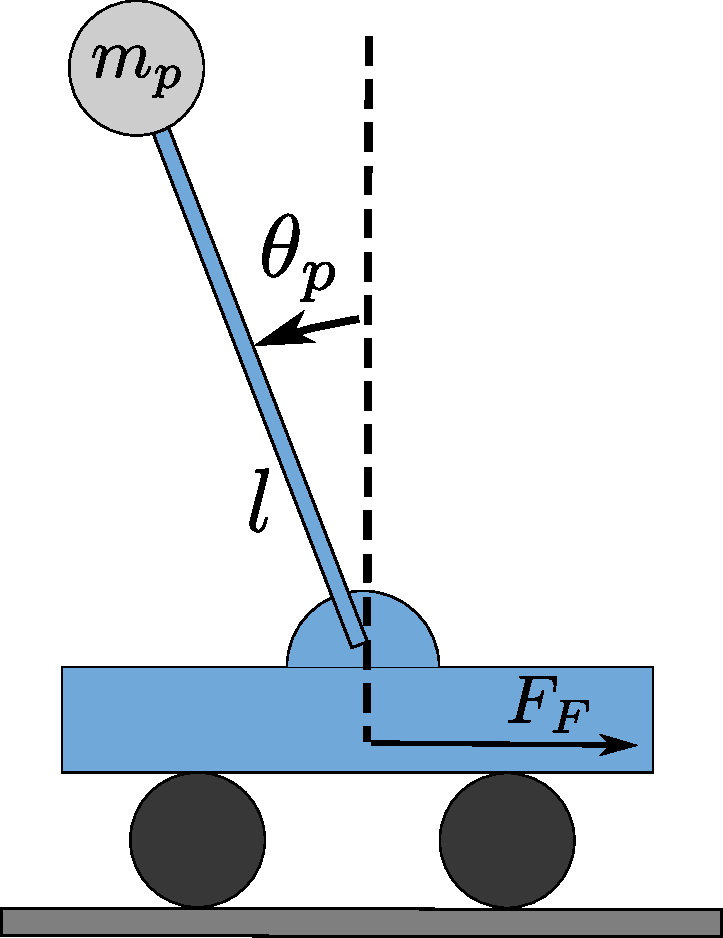
\includegraphics[width=0.4\textwidth]{figures/invertedPendulum.pdf}
%\caption{An inverted pendulum with mass \emph{m} placed on a moving base which is affected by a force $F$. The pendulum has length \emph{l}, and is currently tilted at an angle \emph{$\theta$}}
%\label{fig:invertedPendulum}
%\end{figure}

\begin{figure}[H]
\centering
	\begin{minipage}{0.45\textwidth}

	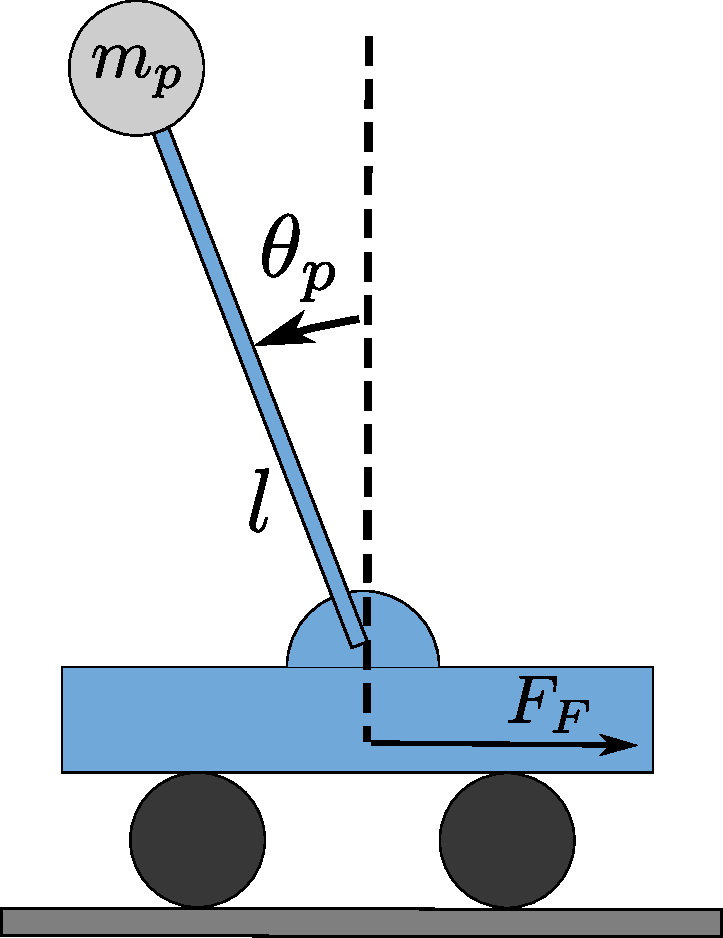
\includegraphics[width=0.9\textwidth]{figures/invertedPendulum.pdf}
	\caption{An inverted pendulum placed on a moving base}
	\label{invertedPendulum}
	\end{minipage}
	\hspace{0.08\textwidth}
	\begin{minipage}{0.40\textwidth}
	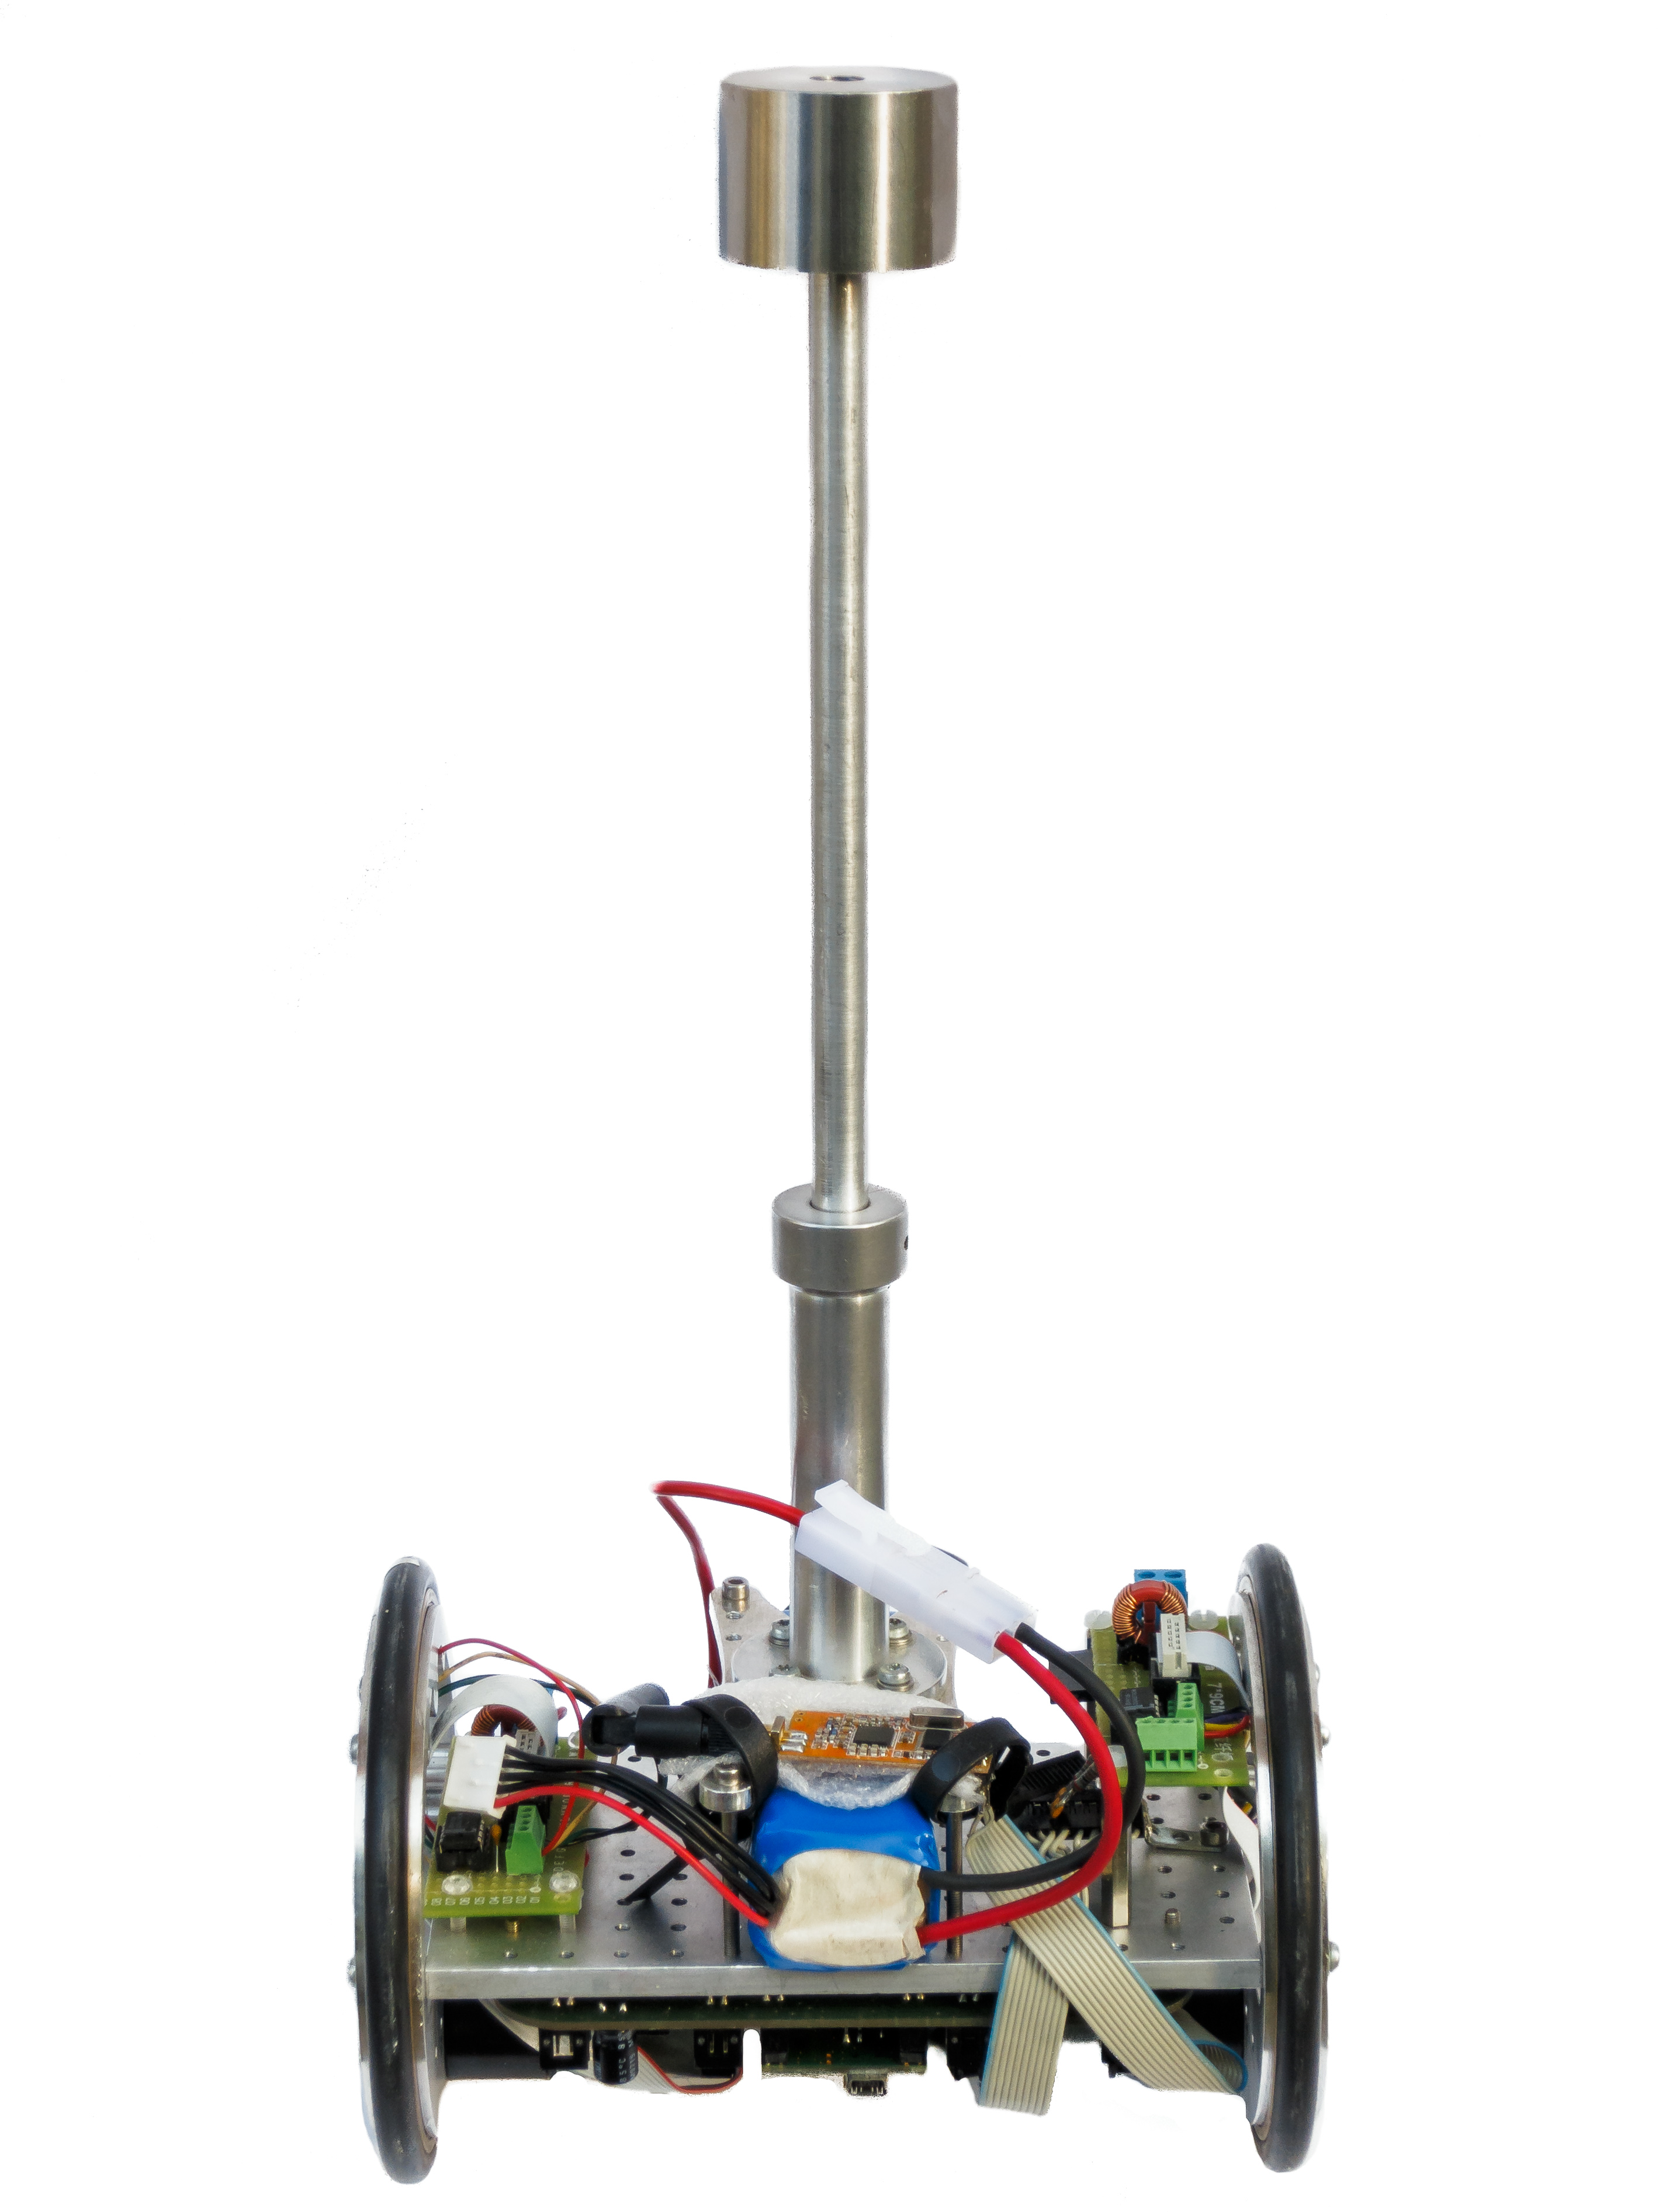
\includegraphics[width=\textwidth]{figures/hardwarePlatform.jpg}
	\caption{The segway to be used in the project (approx. height is 37 cm)}
	\label{minisegway}
	\end{minipage}
\end{figure}
%\todo{why is this interesting to work with}
\vspace{-3mm}
The inverted pendulum has found a new application in recent years, namely in the form of the segway. A segway is a small vehicle that can be used for human transportation where the user stands on a platform placed between two wheels.

%\begin{figure}[H]
%\centering
%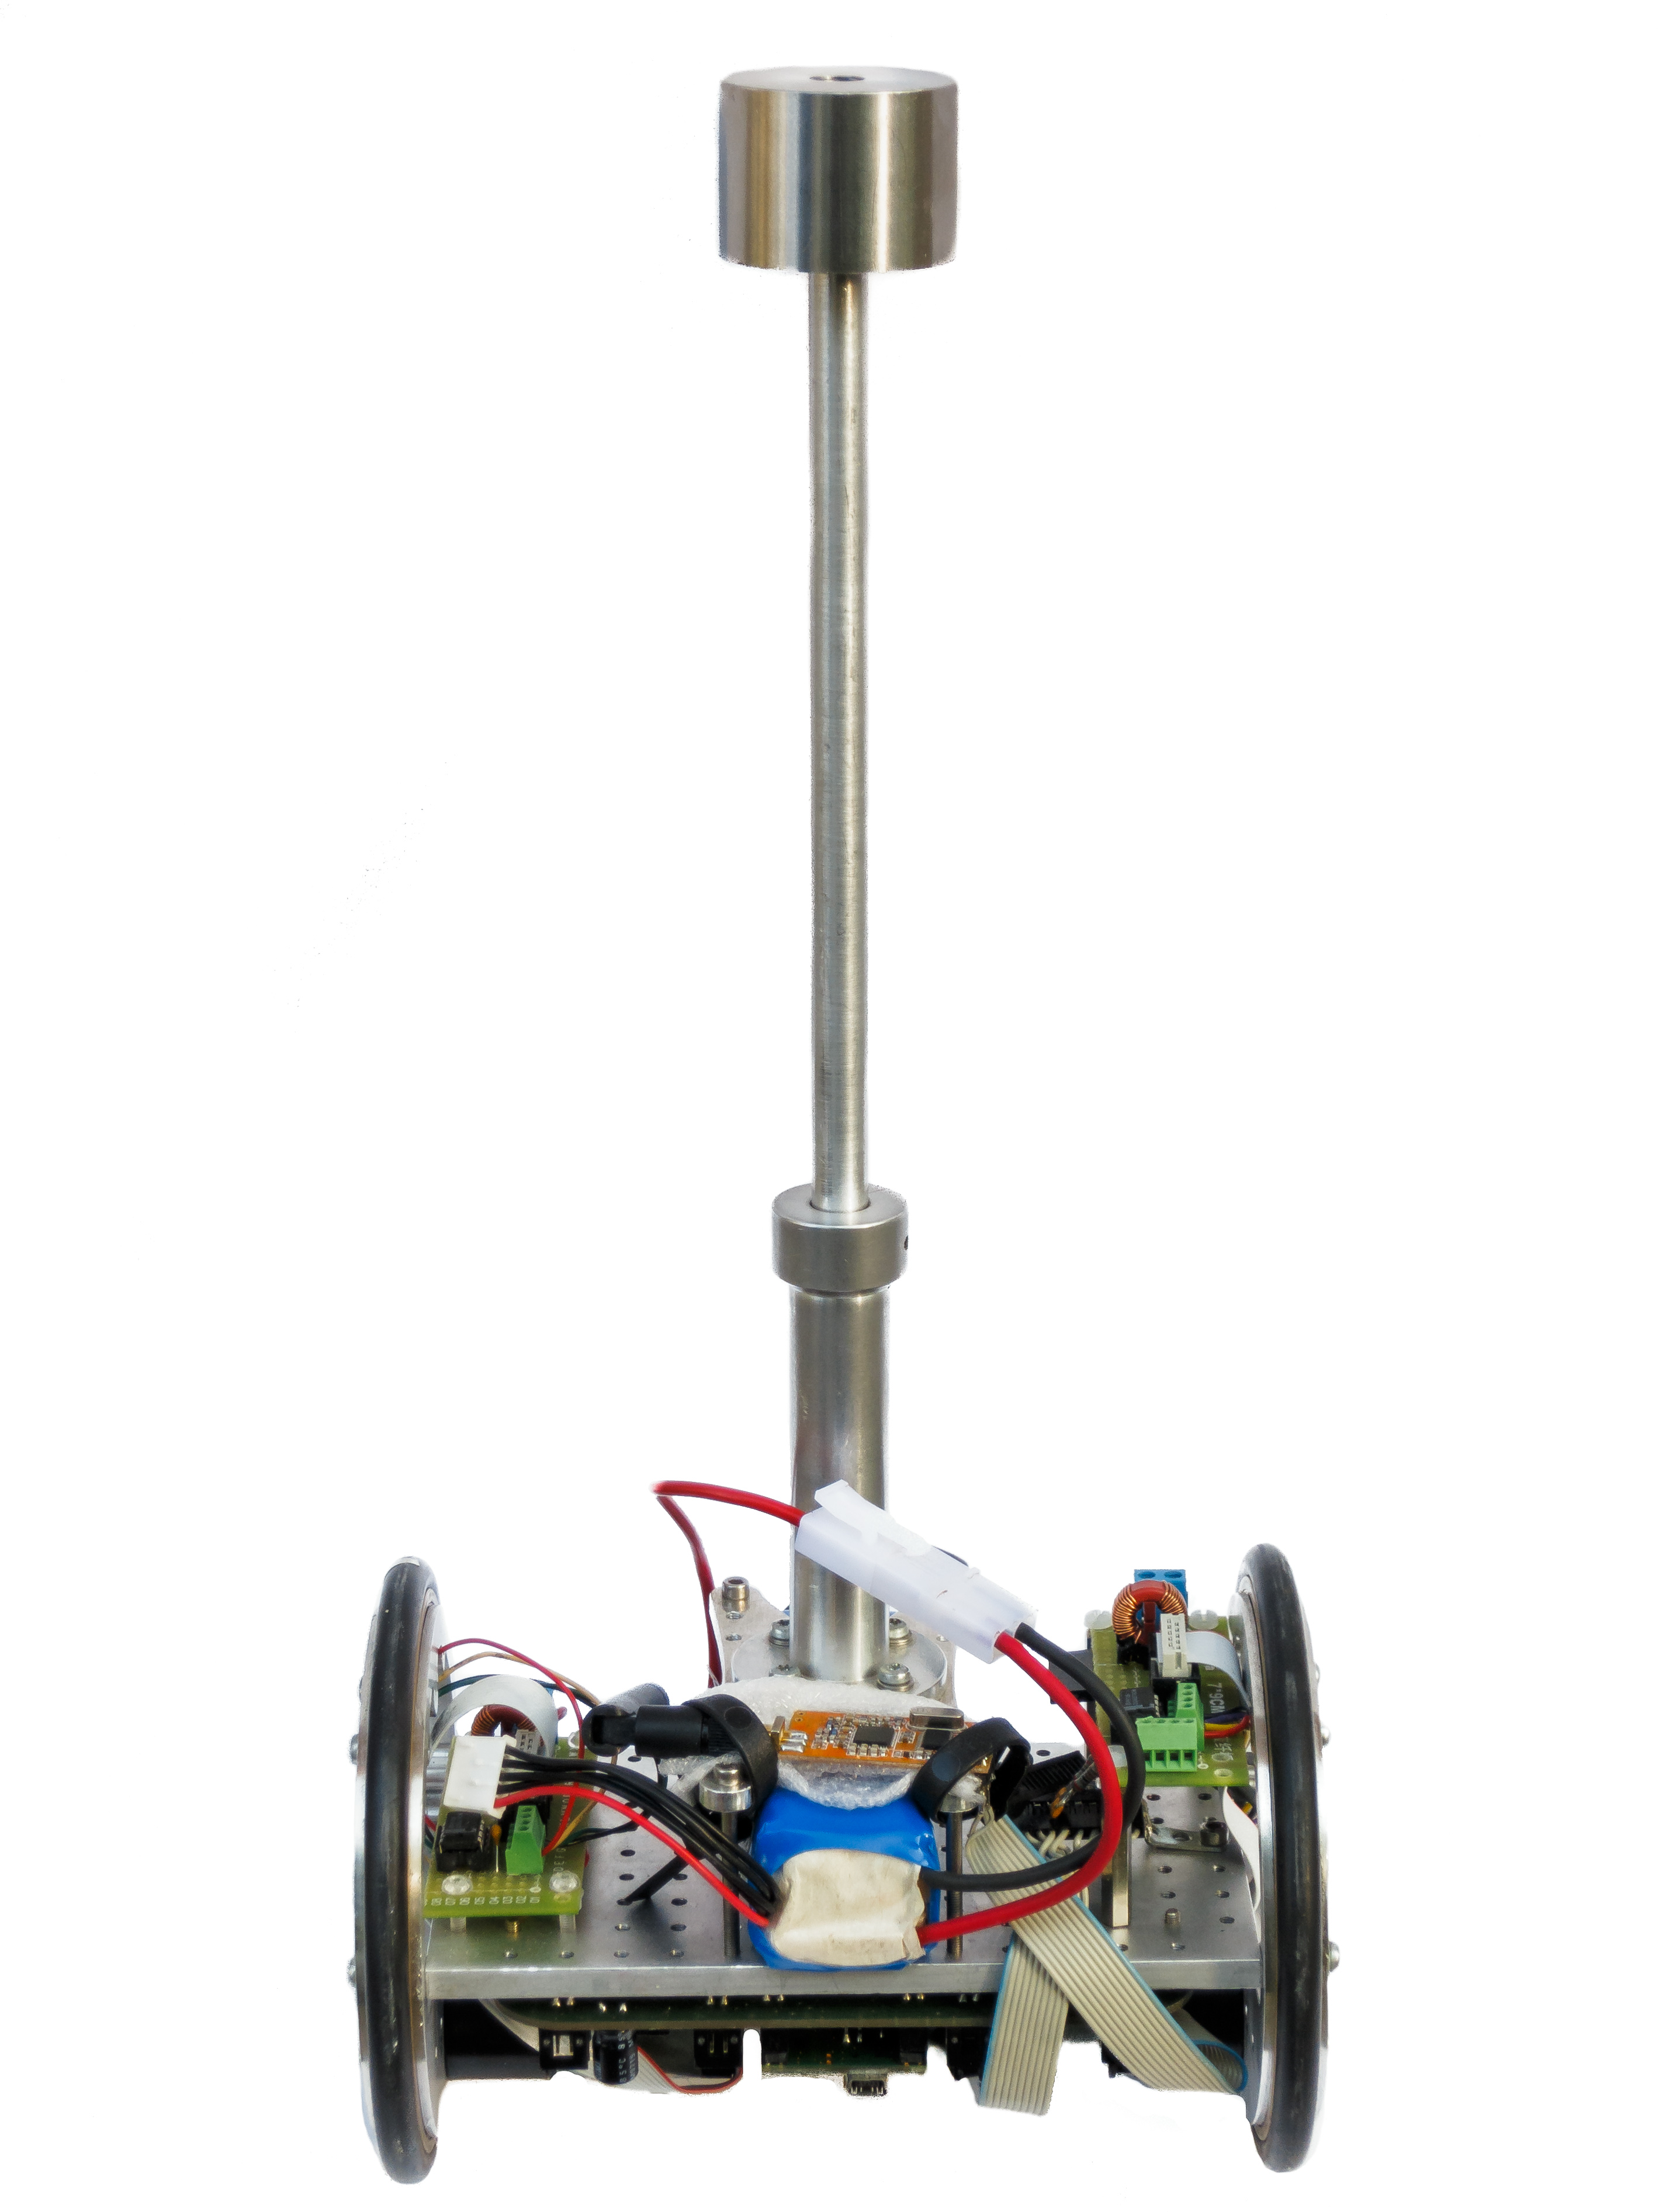
\includegraphics[width=0.4\textwidth]{figures/hardwarePlatform.jpg}
%\caption{The minisegway to be used in the project}
%\label{fig:minisegway}
%\end{figure}

This project concerns the development of a controller for a pre-manufactured segway provided by Aalborg University as can be seen in \autoref{minisegway}. This controller is to stabilize the inverted pendulum in it's upright position, and control the segway's position. The segway is seen as toy to be driven around indoors, and not as a model of a full-size segway. Because of this, all mentions and analyses of a segway throughout the report is in regards to the segway, and not a full-size segway.\\
In the following chapter, a presentation of the general workings of segway is presented.
%In order to control the balancing and driving of the segway, a controller has to be implemented. A good solution is to make the remote control wireless. %Therefore, a wireless remote for the segway will be discussed later on. \todo{a bit rough introduction to remote controller requirement}



%Before the actual modelling and controller design can take place, a presentation of this platform done in the following chapter.


%in particular the modelling and control needed to make the segway self-balancing.
%Ralf's suggestions:

%The inverted pendulum is a classical control problem, in which a pendulum, usually hanging beneath the pivot point, is inverted so that it hangs above.
%
%Whereas a regular pendulum is a stable system with a resting position, the inverted pendulum is inherently unstable. This means that unless some action is taken, the pendulum will fall over by itself. 
%
%The inverted pendulum has found a new application in recent years, namely in the form of the segway. A segway is a means for transportation, where the user stands on a platform placed on two wheels. The segway moves in the direction the user moves, i.e. if the user leans forward, the segway moves forward.
%
%This project concerns the development of a segway, in particular the modelling and control needed to make the segway self-balancing.

%\chapter{Segway Presentation}
In the following chapter, an overview of how a segway works is presented. This includes a block description of the system, and a description of the functionalities	 it is to have.
The segway provided by Aalborg University is also described, in regards to the mechanical frame and the provided hardware.

\section{Generalized Segway Description}
A segway can be seen as a typical control system, as shown in \autoref{fig:seg_over}.
Here, the controlled parameters are acquired using various transducers, processed by the system controller and then a control signal is outputted to the actuator(s) through. Apart from the control system, a \gls{RC} is added to the system, which can also be seen in \autoref{fig:seg_over}. The reason for this will be described later on. In the case of the segway, the transducers are sensors, providing information on the movement of the segway, and the actuators are motors, which are driving the wheels. 

\begin{figure}[H]
\centering
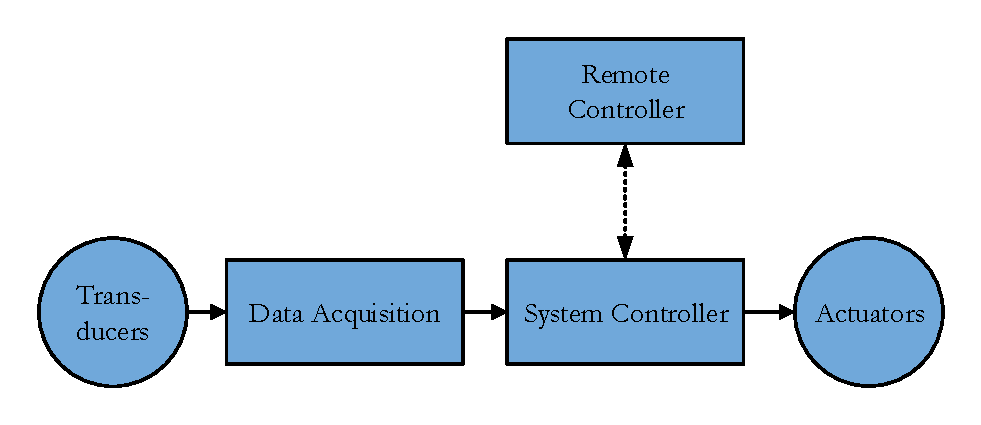
\includegraphics[width=0.7\textwidth]{figures/segwayOverview.pdf}
\caption{Generalized block diagram of a segway control system.}
\label{fig:seg_over}
\end{figure}

It is decided that the segway is to have four main functionalities to function as desired. These functionalities are \textit{balancing, driving, turning and the ability to be remote controlled}. Each of these are described in further detail in the following section.

\subsection{Functionalities of the System Controller}
The controller unit has four main functionalities, namely balancing, driving, turning, and transceiving wireless signals between the \gls{RC} and the system controller. Each of these functionalities are described in further detail in the following section.

One of the required functionalities of any segway is the ability to balance. The system controller must control the motors so the inverted pendulum is balancing vertically. Because the pendulum is unstable by nature, the controller has to make the system stable. This functionality relies on input from the transducers, which is used to calculate an actuator signal to keep the segway balanced.

%The movement and control of the system can be based of the current state of the segway measured by transducers. The transducers can for example tell about the current position, speed, and acceleration of the segway. 

%The data will then be processed in the microcontroller which determines how the segway should react to the current state.

%\subsubsection{Transceiving of wireless commands}
Through a wireless RC the segway is remote controlled. This means that the segway must be capable of receiving commands from the RC and make the segway move accordingly. To achieve this, the segway and RC must share a communication protocol. The wireless RC should also able to receive information regarding the movement of the segway like the speed, angular velocity and angle.

%\subsubsection{Driving and turning}
The driving and turning functionalities are responsible for controlling the segway's forward and backwards velocity as well as the direction of the segway. To ensure the segway does not fall over when driving or turning, the movement will of course have to happen in corporation with the balancing functionality, since balance is still to be kept when driving and turning.

%The velocity of the segway can be controlled by changing which angle the balance functionality tries to uphold. To keep this new angle, the balance functionality must respond to the change in angle, by changing the translatoric velocity. In other words, the rotational moment must be countered by an equal translatoric force.

%Unlike the driving functionality, the turning functionality does not lead to changes in the balance functionality, since turning is rotation around a different axis.

%These functionalities are in the same control unit as they must correlate with the balance functionality, since the output of both the balance, driving and turning functionalities must be merged before it is sent to the motor control unit.

%%\chapter{System presentation}
%Aalborg University has provided the project group with a pre-built mini segway. Based on the system design of an segway this chapter will, present and describe the mini segway, with a focus on the mechanical frame and the provided hardware. 
\section{Description of Provided Segway} \label{sec:hardware}
Before the modelling and the design of the controller can begin, the segway provided by the university first has to be described, especially in regards to the electronic hardware used on the segway. This is done in the following section. A photo of the provided segway can be seen in \autoref{hardwarePlatform}. 

\begin{figure}[H]
	\centering
	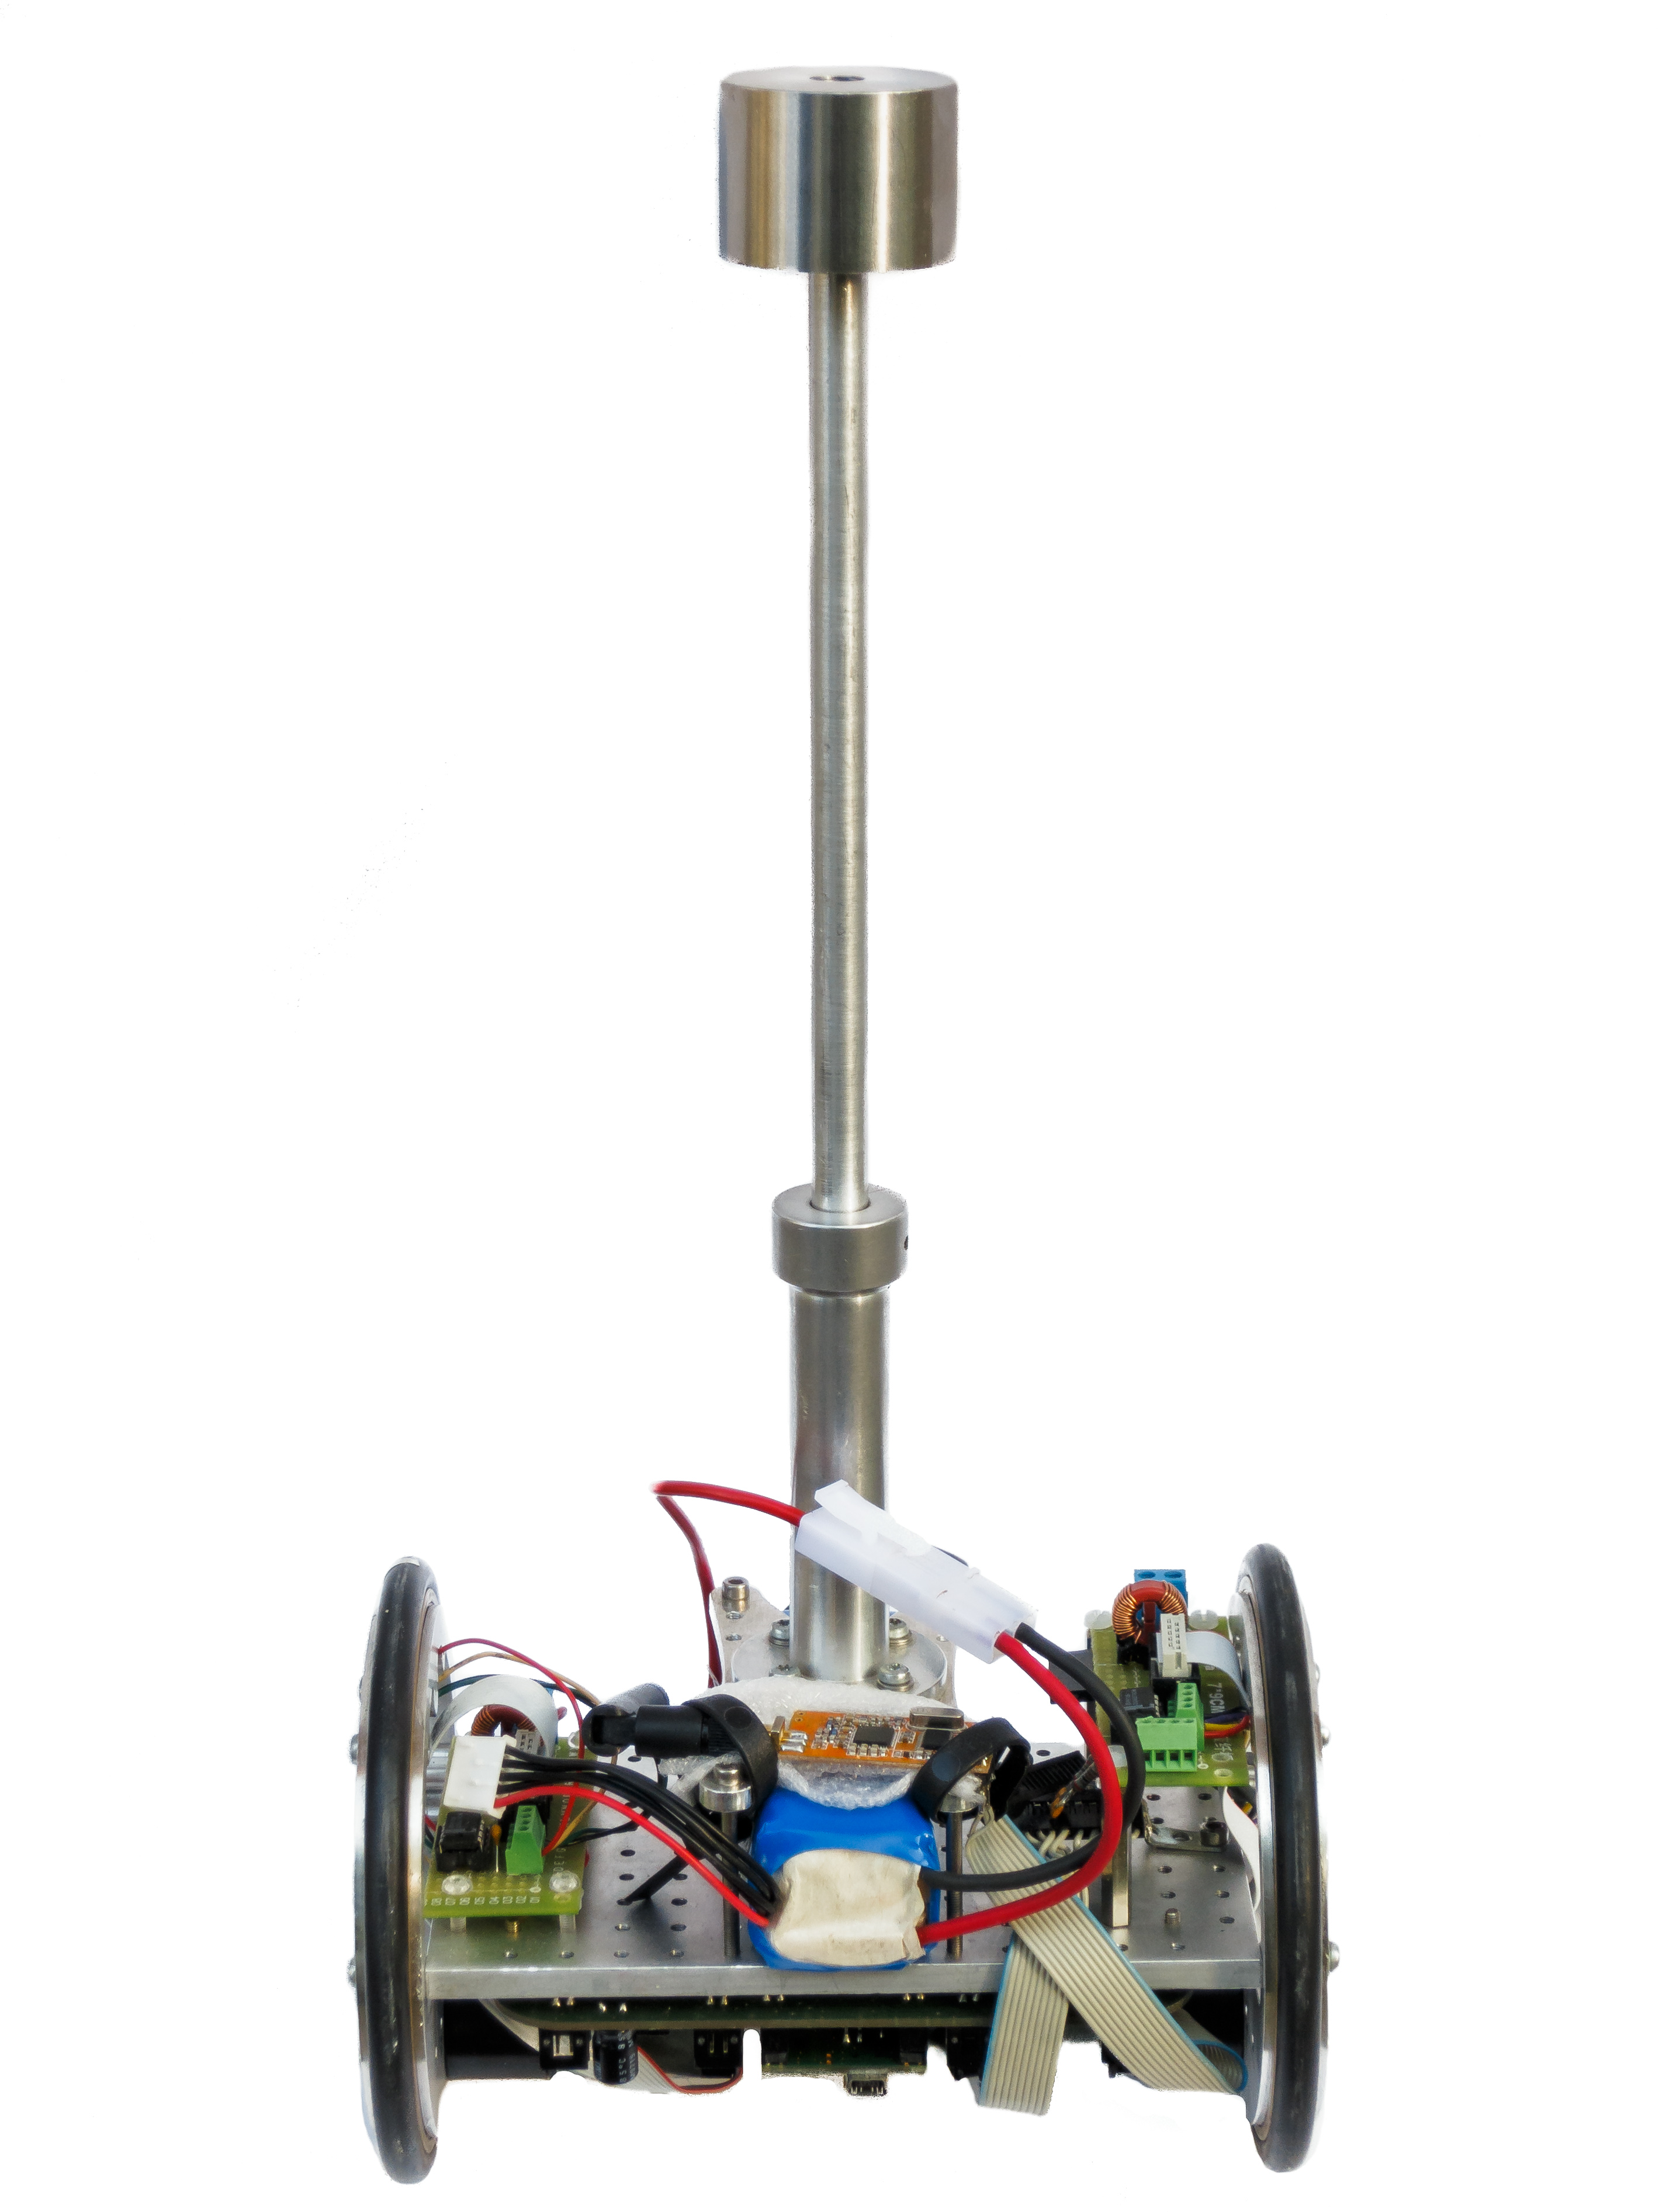
\includegraphics[width=0.4\textwidth]{figures/hardwarePlatform.jpg}
	\caption{The segway to be used in the project.}
	\label{hardwarePlatform}
\end{figure}

The segway consists of several items, these items are divided into 3 main groups, namely \textbf{mechanical}, \textbf{power} and \textbf{electronics}. These groups and the items they include are described in the following.

%\begin{itemize}
%
%\item \textbf{Mechanical}
%\begin{itemize}
%\item Mechanical frame
%\item Wheels
%\item Motors
%\end{itemize}
%
%\item \textbf{Power}
%\begin{itemize}
%\item Batteries
%\item PSUs (Power Supply Units)
%\end{itemize}
%
%\item \textbf{Electronics}
%\begin{itemize}
%\item Wireless transceivers
%\item Microcontroller
%\item Filters
%\item Accelerometer + gyroscope
%\item Motor driver
%\item Encoders
%\end{itemize}

%\end{itemize}
%\todo{remove list, write as text}
%These will be described in further details in the following.

\subsection{Mechanicanics}
\subsubsection{Mechanical Frame}

The provided segway's mechanical frame is made from aluminium. It consists of a baseplate onto which the wheels are mounted, together with a rod with a cylindrical mass on top. All electronics including batteries are mounted on the baseplate.

A blueprint of the segway can be seen in \autoref{segwaySchematic} in \appref{app:segwayParameters}, and measurements of relevant parameters of the frame is listed in \autoref{tab:dimensions}, also in \appref{app:segwayParameters}.


%\begin{wrapfigure}{R}{0.5\textwidth}
%\centering
%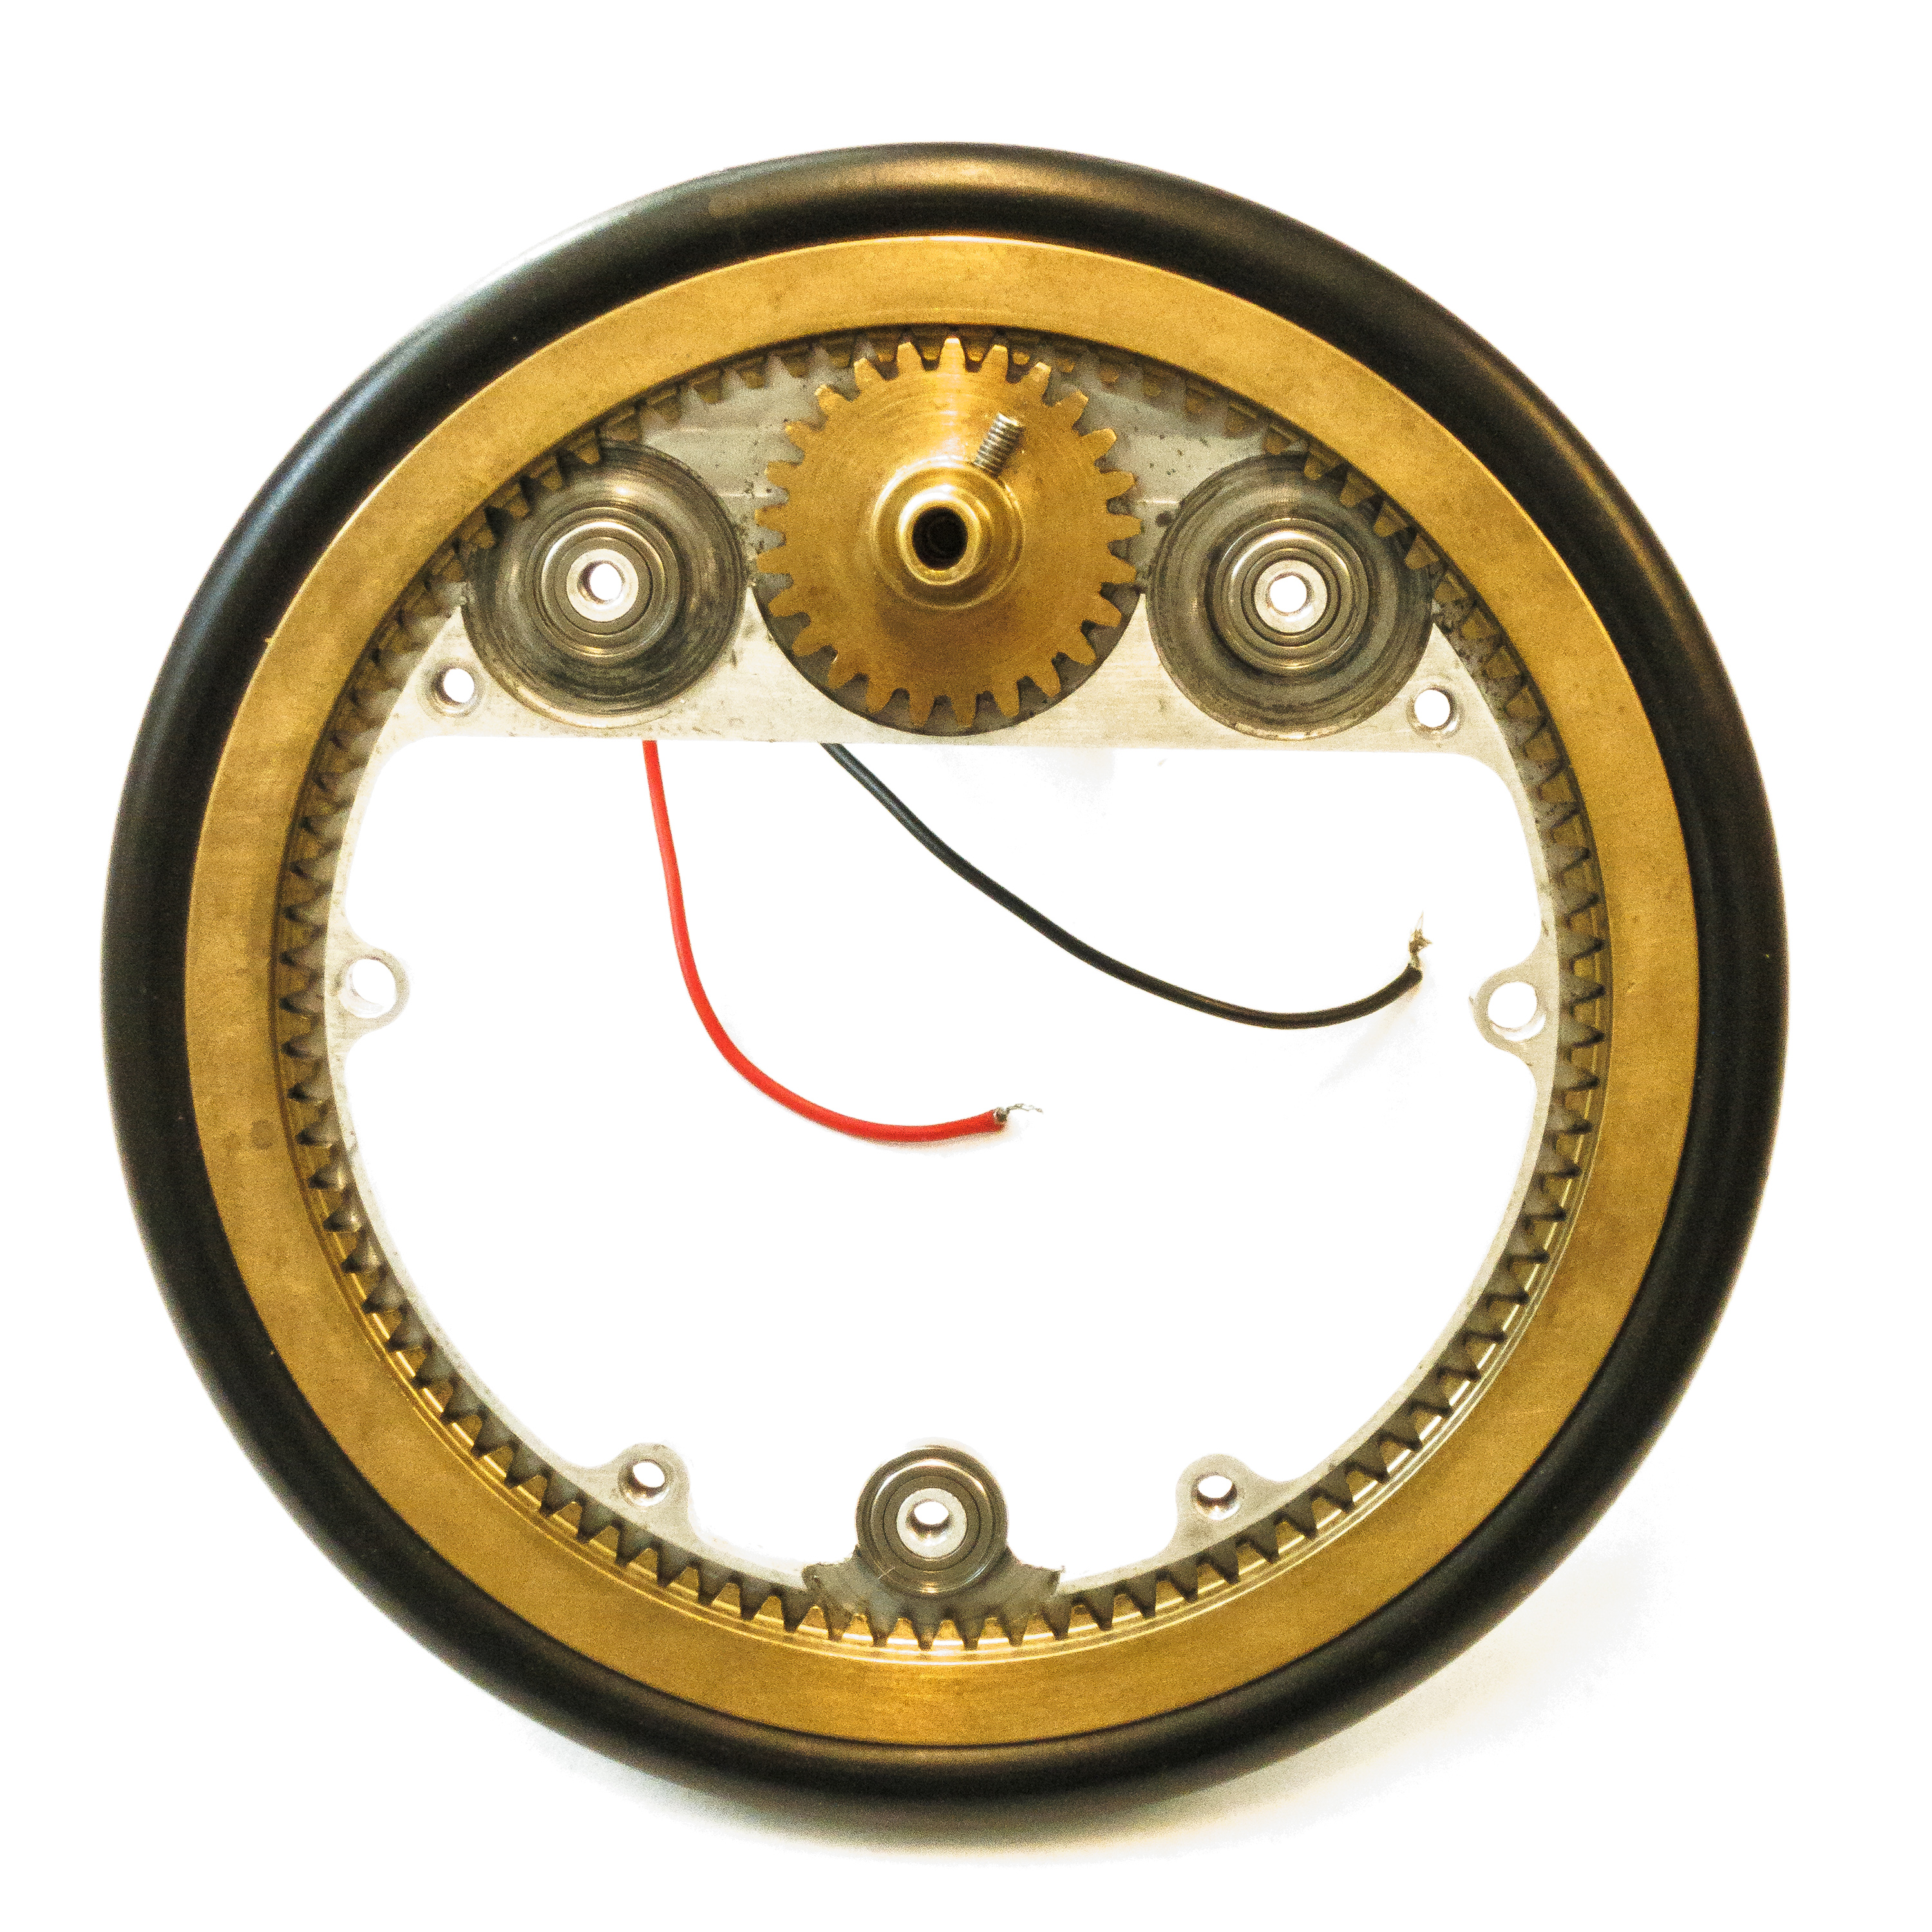
\includegraphics[width=0.4\textwidth]{figures/wheel.jpg}
%\caption{The wheel and motor showing the transmission(motor behind the small gear)}
%\label{fig:wheel}
% \vspace{-4cm}
%\end{wrapfigure}


\subsubsection{Wheels}
\label{subsec:wheels}
The wheels mounted on the segway feature an offset motor, meaning the motor is not mounted at the center. Though, as seen from the blueprint in \autoref{segwaySchematic} in \appref{app:segwayParameters}, the axis of the wheel is still in the center of the base. The wheel system is built as follows: The motor rotates a gear fitted onto the motor from the factory. The shaft from this gear is located on the inner side of the wheel, and mounted to a cogwheel. The inner side of the wheel itself has some small cogs making it the other part of the transmission system.
For a better rotation and less friction, the wheel has three ball bearing guides. This can be seen in \autoref{fig:wheel}.
The cogwheel mounted on the motor wheel has 25 cogs and the inside of the wheel has 90 cogs.

\begin{figure}[H]
\centering
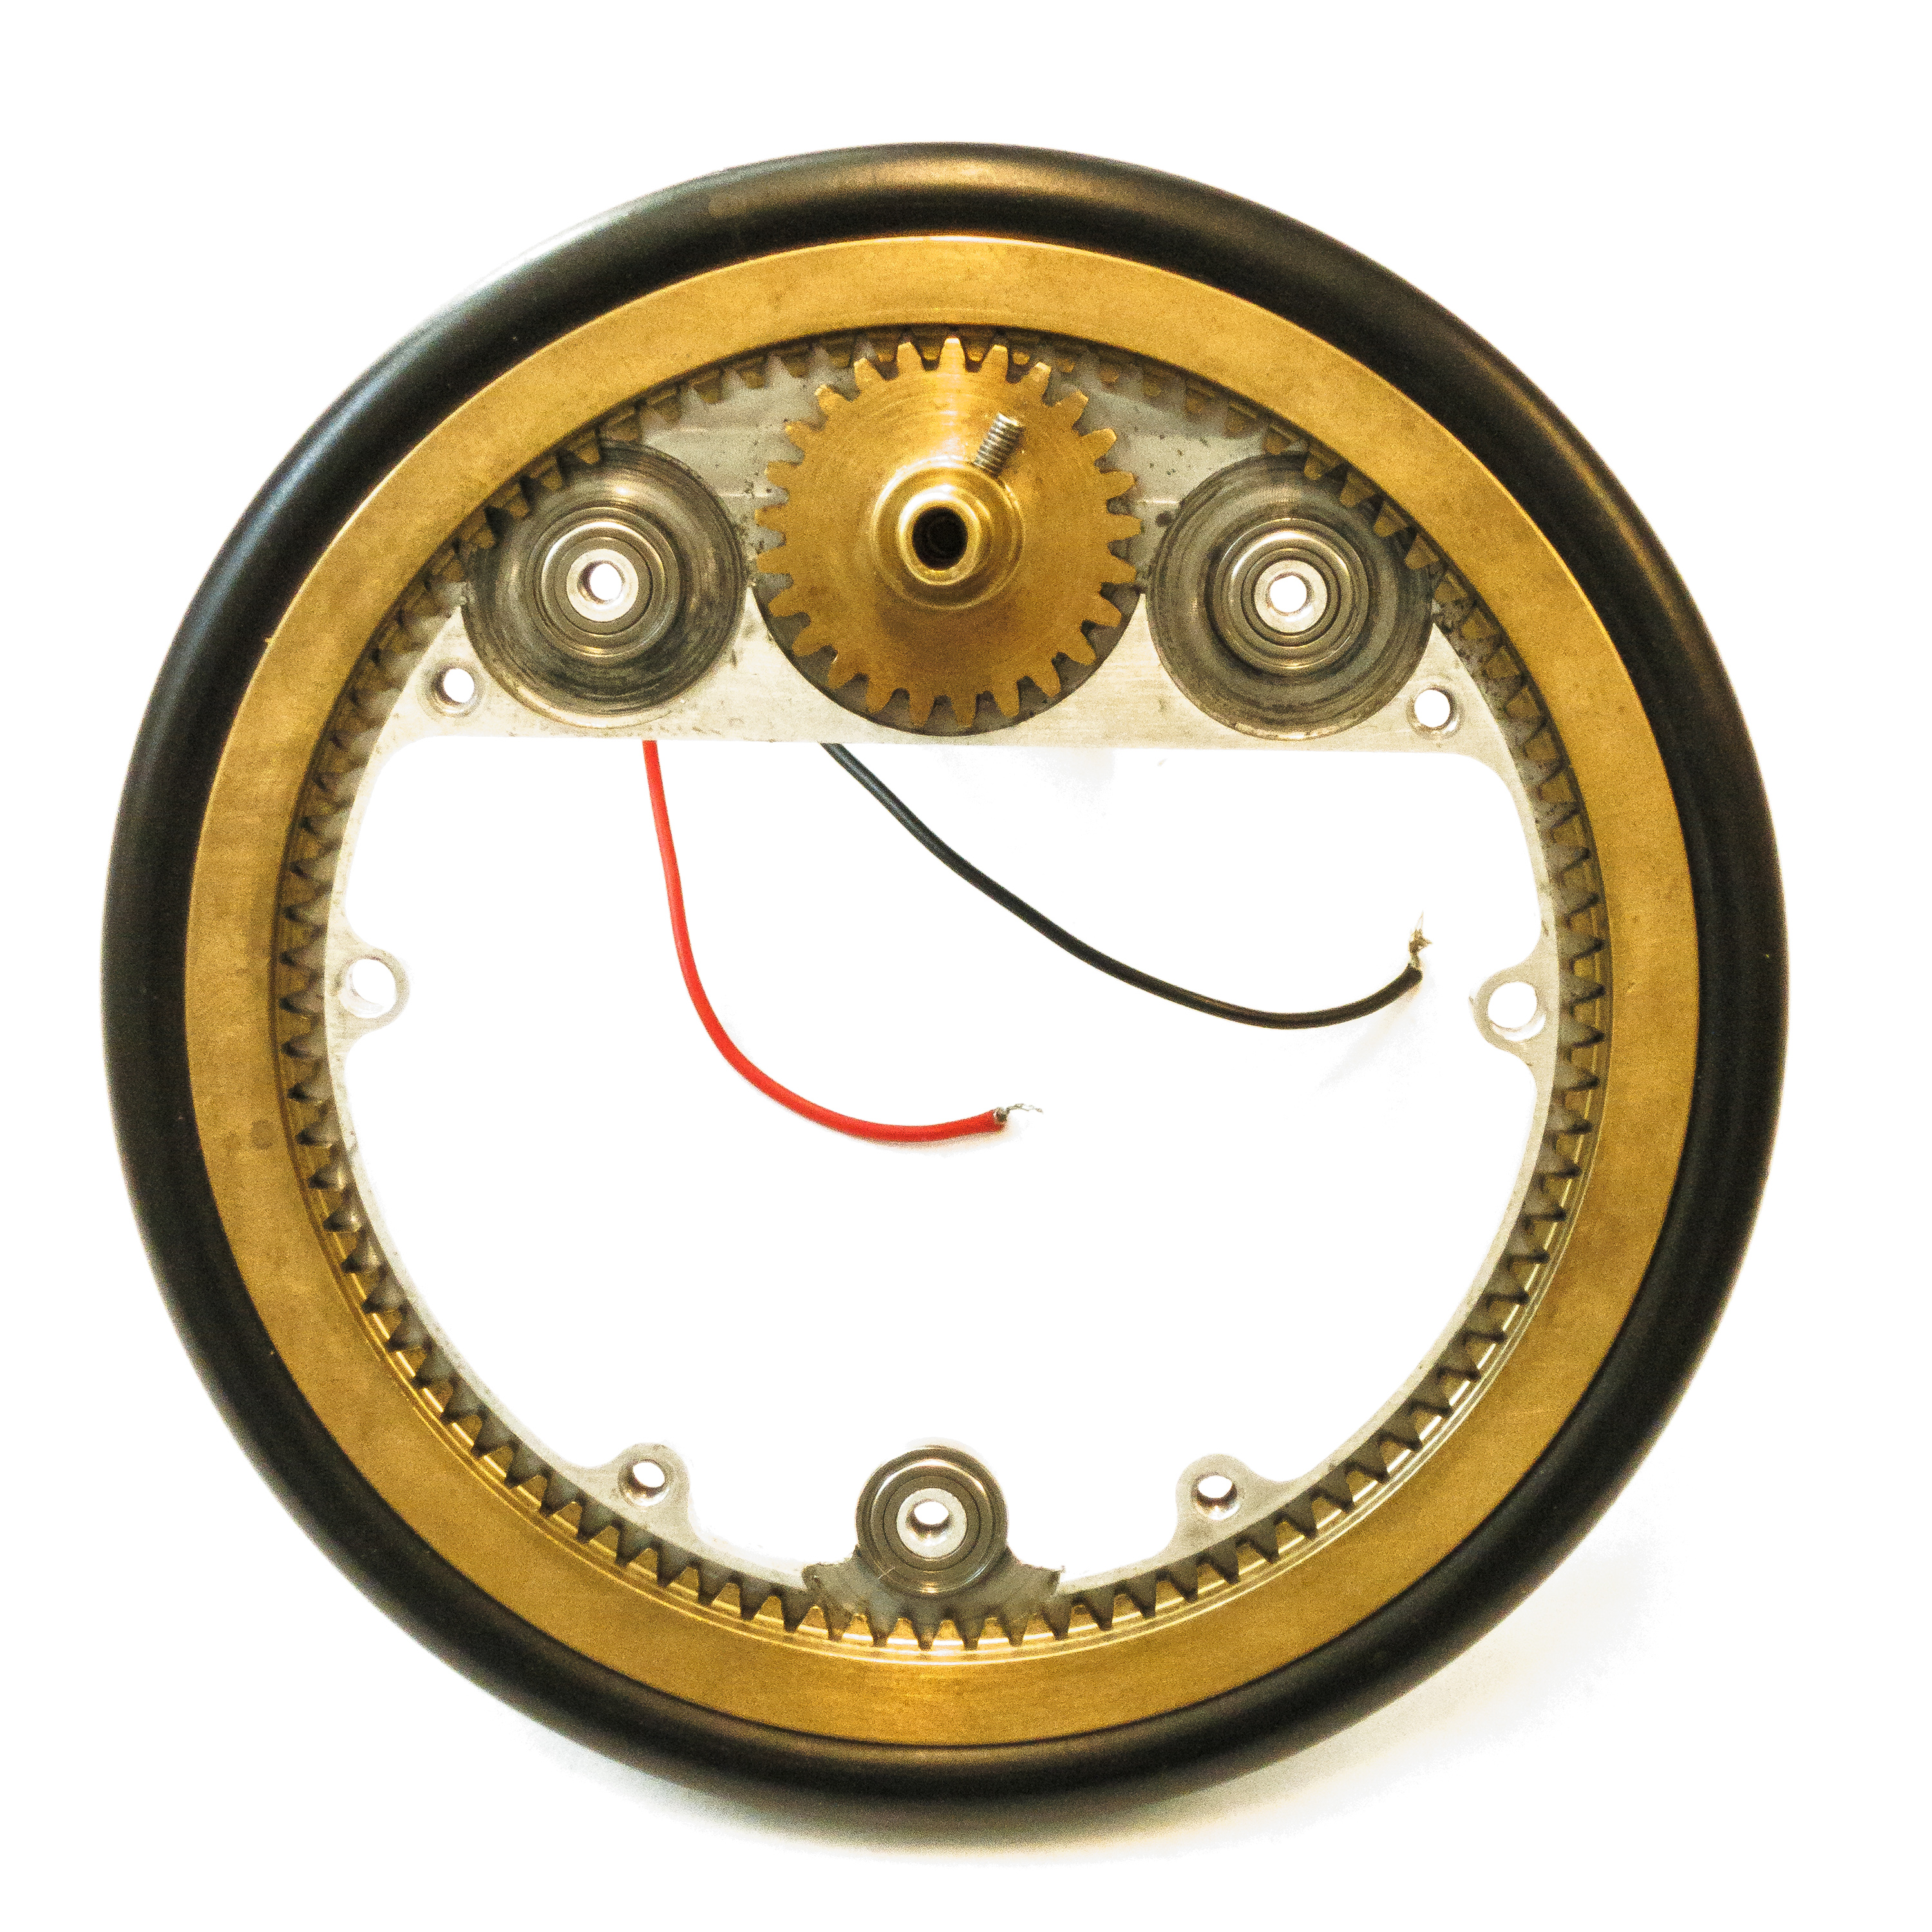
\includegraphics[width=0.4\textwidth]{figures/wheel.jpg}
\caption{The wheel and motor showing the transmission. The motor is behind the small gear.}
\label{fig:wheel}
\end{figure}

\subsubsection{Motors}
\label{subsec:motors}
The segway uses two Maxon A-Max 110160 permanent DC-motors to rotate the wheels. Parameters of the motors that might be taken into account are the rotational speed and the torque. The specification of the motors are \citep{maxon}
\begin{itemize}
\item Nominal torque at {6 V} is 5.91 mNm.
\item Nominal speed at {6 V} is 6240 RPM.
\end{itemize}

%A permanent DC motor is working by rotating an armature within a magnetic field. This produces a mechanical force, when a current carrying conductor is placed in the magnetic field, as this is exerting an equal and opposite force due to Newton's third law. 

%The rotational speed is given in RPM (Revolutions Per Minute) and the torque is given in mNm (milli Newton meter).

The motors are brushed, meaning the stator corresponds to the magnets and the rotor is composed of the coils, receiving power through brushes.
Brushed motors have important advantages: They have a low cost of construction, require only simple and inexpensive control and they operate in extreme environments due to lack of electronics. However, those motors also have drawbacks: They require periodic maintenance, their characteristics are moderately flat and at high speeds, brush friction increases, thus reducing useful torque. Also, the brush arcing will generate noise causing electrical magnetic interference (EMI) \citep{BvsBL} \citep{BvsBLv2}.

\begin{figure}[H]
	\centering
	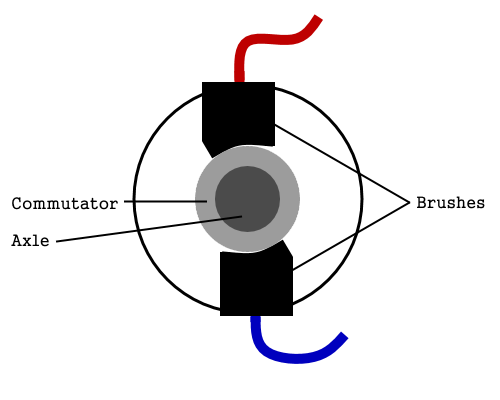
\includegraphics[width=0.5\textwidth]{figures/brushed_2.png}
	\caption{Sectional view of a brushed motors.}
	\label{DCBrushed}
\end{figure}

As a part of the motors, a gear (Maxon 110356) has been fitted on the motor. This gear was fitted from the factory, and the inner workings of it are therefore not known. From the datasheet, the gear ratio between the motor and shaft is known \citep{gear}: 
$$N_{ms} = \frac{1}{19} \approx 0.053$$

\subsection{Power}
\subsubsection{Batteries}
The segway comes equipped with a battery which is the source of power of the system. The battery is a rechargeable 4S LiPo. LiPo batteries, or Lithium-ion Polymer batteries, consists of cells in series, \textit{x}S meaning \textbf{\textit{x}} cells in \textbf{S}eries. A LiPo cell has a nominal voltage of 3.7V. The battery used on the device has a nominal voltage of 14.8 V (3.7 Volts times 4 cells).
LiPo batteries, compared to other types such as Nickel–metal hydride (NiMH), one of the most common battery types, are lighter and more compact. However, they are more expensive than "regular" batteries and require a specific charger to bring every cell of the pack to the same state of charge \citep{Cells}.

The Segway also has two Power Supply Units (PSU's). These are electronic components, whose role it is to regulate the unstable input voltage from the batteries, to a stable voltage to be used by the electronics.
One has an output of 5V and the other has an output of 3.3V. 

\pagebreak 
\subsection{Electronics}
\subsubsection{Wireless Transceivers}
To facilitate the wireless communication between the segway and a remote controller, a pair of APC220 radio communication modules is supplied.
The modules have the following features \citep{wifimodule}:
\begin{itemize}
\item Transmission distance of up to 1000 m (2400 baud)
\item UART/TTL interface with 256 bytes data buffer
\item -112 dBm sensitivity at 9600 baud
\item 20 mW output power
\item Adjustable frequency from 418 MHz to 455 MHz
\end{itemize}

Since the modules have a UART interface, they can be interfaced through a UART interface on a microcontroller, which makes the radio modules simple and easy to use.

\subsubsection{Microcontroller}

A microcontroller board is supplied with the segway. The \gls{PCB} on which all the electrical components are mounted, is designed to fit the supplied \gls{MCU}, and thus a new MCU is not chosen, since it might require a redesign of the PCB.

The microcontroller board supplied is a \emph{CrumbX128A3} made by Chip45 \citep{CrumbX128A3}. The CrumbX128A3 features an ATxmega128A3U microcontroller, a 3.3V low dropout (LDO) voltage regulator, a USB UART converter, an RS485 transceiver and a micro-sd-card header/slot.
	
The ATxmega128A3U has the following specifications \citep{xmega}:

\begin{itemize}
\item 32 MHz clock speed
\item $1.6-3.6$ V power supply
\item 128 Kb flash
\item 8 KB SRAM
\item 7 UARTs
\item 7 16-bit counters
\item 4-channel DMA controller
\end{itemize}
\subsubsection{Accelerometer and Gyroscope}
To measure the angle the segway is tilted as well as its relative position, an accelerometer and gyroscope is used. Here, the InvenSense MPU-6050\citep{gyro} is used, a 6-axis gyroscope and accelerometer. The chip is implemented on a GY-521 breakout board. It features an \iic bus, from which the raw sensor values can be read. 
The gyroscope can be configured to having a full-scale range of either $\pm 250, \pm 500, \pm 1000$ or $\pm 2000 \degree /\text{sec}$. The accelerometer can be programmed to have a full-scale range of $\pm 2g, \pm 4g, \pm 8g$ or $\pm 16g$ \citep{gyro}.

\subsubsection{Motor Driver}
To control the motors, a motor driver is used, in form of an H-bridge. The H-bridge allows a small controller-voltage to control a (often relatively large) current. This is practical, since the current needed to drive most motors is bigger than what can be drawn from the pins of a microcontroller. 
Here, two Freescale MC33926 5A H-bridges \citep{hbridge} are supplied - one for each motor. The H-bridge makes it possible for a motor to be run both forward and backwards, based on the input signals to the chip. It also features a feedback-pin, also known as a current sense, that can be used to measure the current drawn by the motor. The H-bridge is controlled by an input PWM signal and two direction pins. By setting these pins, the motor can be either locked, free-running or moving forwards or backwards.

\subsubsection{Encoders}\label{subsec:preEncoder}
In order to keep the inverted pendulum in balance, the segway needs a way to quantify the amount of rotation on the wheels and, by extension, on the motors, hence the encoders. The ones currently used by the system are relative (or incremental) encoders placed directly on the motors.
An incremental encoder delivers a certain number of pulses per revolution. This number of pulses measures the angular movement.
Usually, relative encoders consist of a disc divided in transparent and opaque segments. Most of those discs are equipped with two rows of segments plus a top segment. Both segment tracks are slightly out of phase to indicate the direction of rotation and the additional top segment allows the count of revolutions.
An incremental encoder's resolution corresponds to the maximum number of pulses sent per revolution and is symbolised by the unit "points per rotation" \citep{IncEnc}.
\vspace{-1 cm}
\begin{figure}[H]
	\centering
	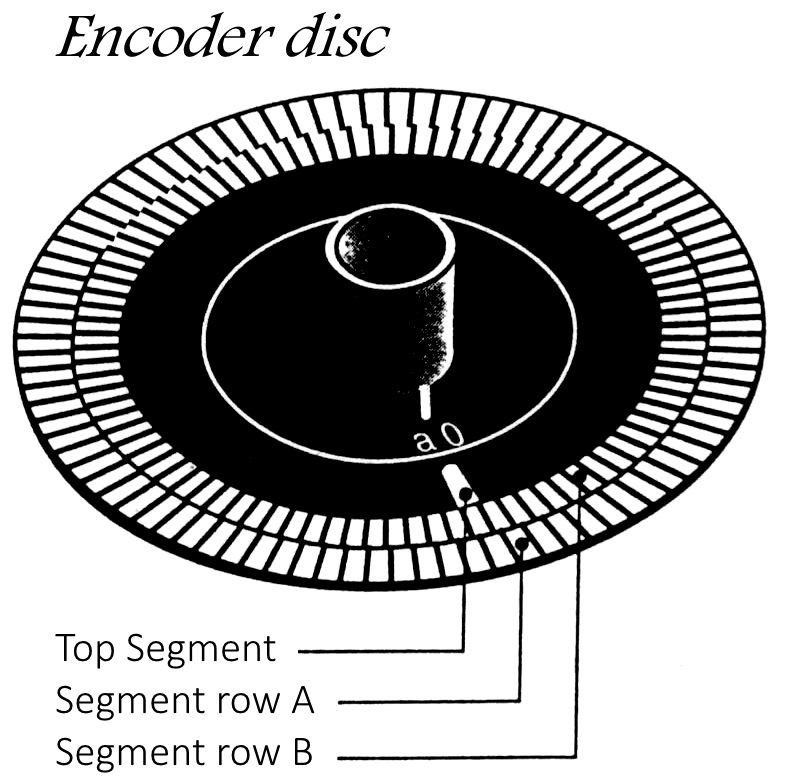
\includegraphics[width=0.36\textwidth]{figures/Encoder.jpg}
	\caption{Detailed scheme of an incremental encoder \citep{IncEnc}.}
	\label{fig:incremental_encoders}
\end{figure}

%Placed between the motor encoders and the microcontroller, are some filters. The filter type used is not known, nor is the filter specifications. Since its inputs and outputs are unknown, it is considered a black box.
%Because of this, it is decided to remove these filters and design new filters, so the exact transfer function of them is known.

\newpage
\subsection{Detailed Segway Overview}
The general block diagram of the segway control system in \autoref{fig:seg_over} can be extended based on the provided hardware described above. The detailed diagram can be seen in \autoref{fig:ext_seg_over}.

\begin{figure}[H]
\centering
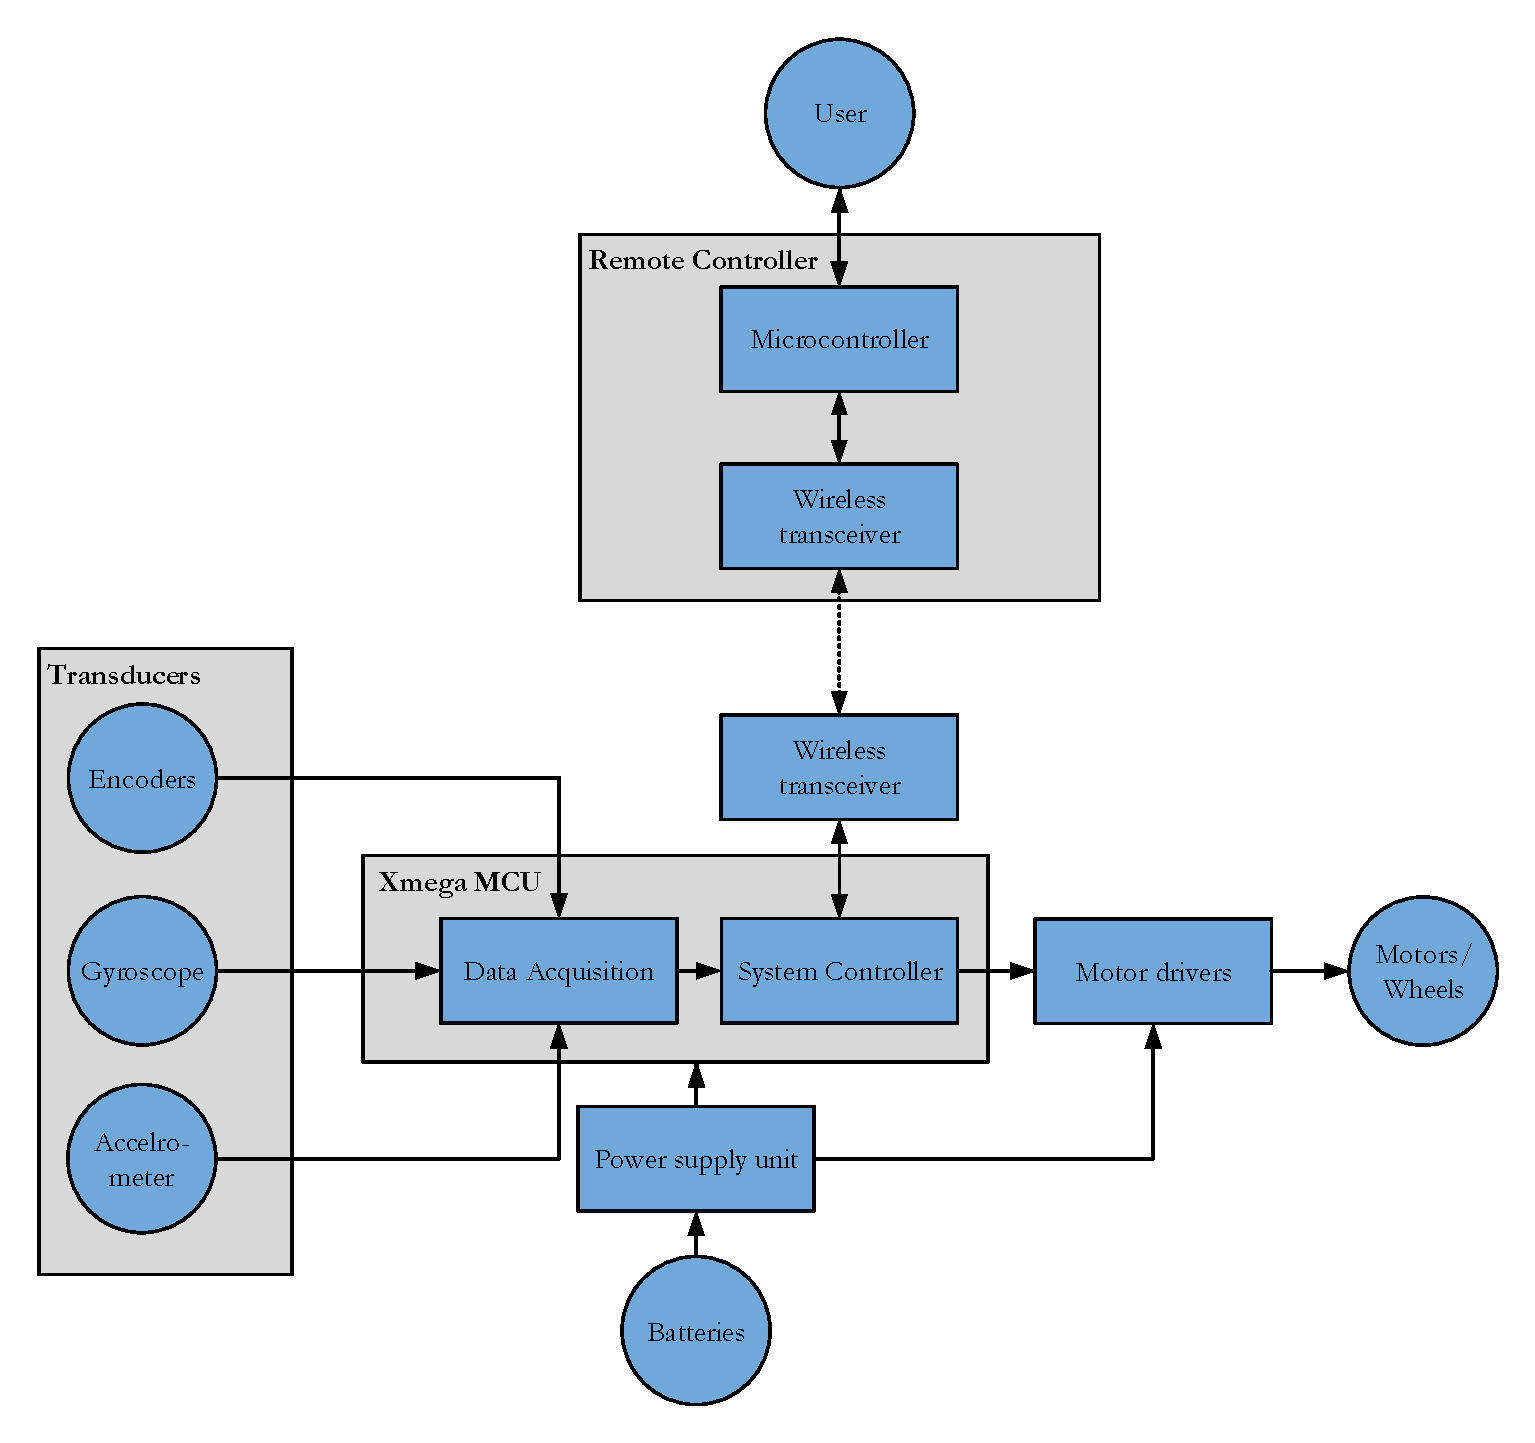
\includegraphics[width = 0.95\textwidth]{figures/extendedOverview.pdf}
\caption{Detailed block diagram of the segway system.}
\label{fig:ext_seg_over}
\end{figure}

In the detailed diagram, the different transducers have been added, and the functionalities the MCU is to facilitate have been grouped. Also, the actuator has been specified, in the form of motors.
The workings of the remote controller are also described in further details, namely that it is to receive user input to a MCU and then transmit it wirelessly. It can also display data from the segway to the user. Also added to \autoref{fig:ext_seg_over} are the batteries and PSUs. 


%\section{System Overview}

Before the design of segway can begin, it has to be determined which subsystems are to be designed. In \autoref{fig:ext_seg_over}, the detailed block diagram of the system was presented. As most of the hardware for the segway is already provided, the project will primary focus on designing the controllers in the system. This limitation can be seen in \autoref{fig:system_overview_block}. Here, the blue blocks are subsystem that are to be designed, while the grey blocks are not designed.


\begin{figure}[H]
	\centering
	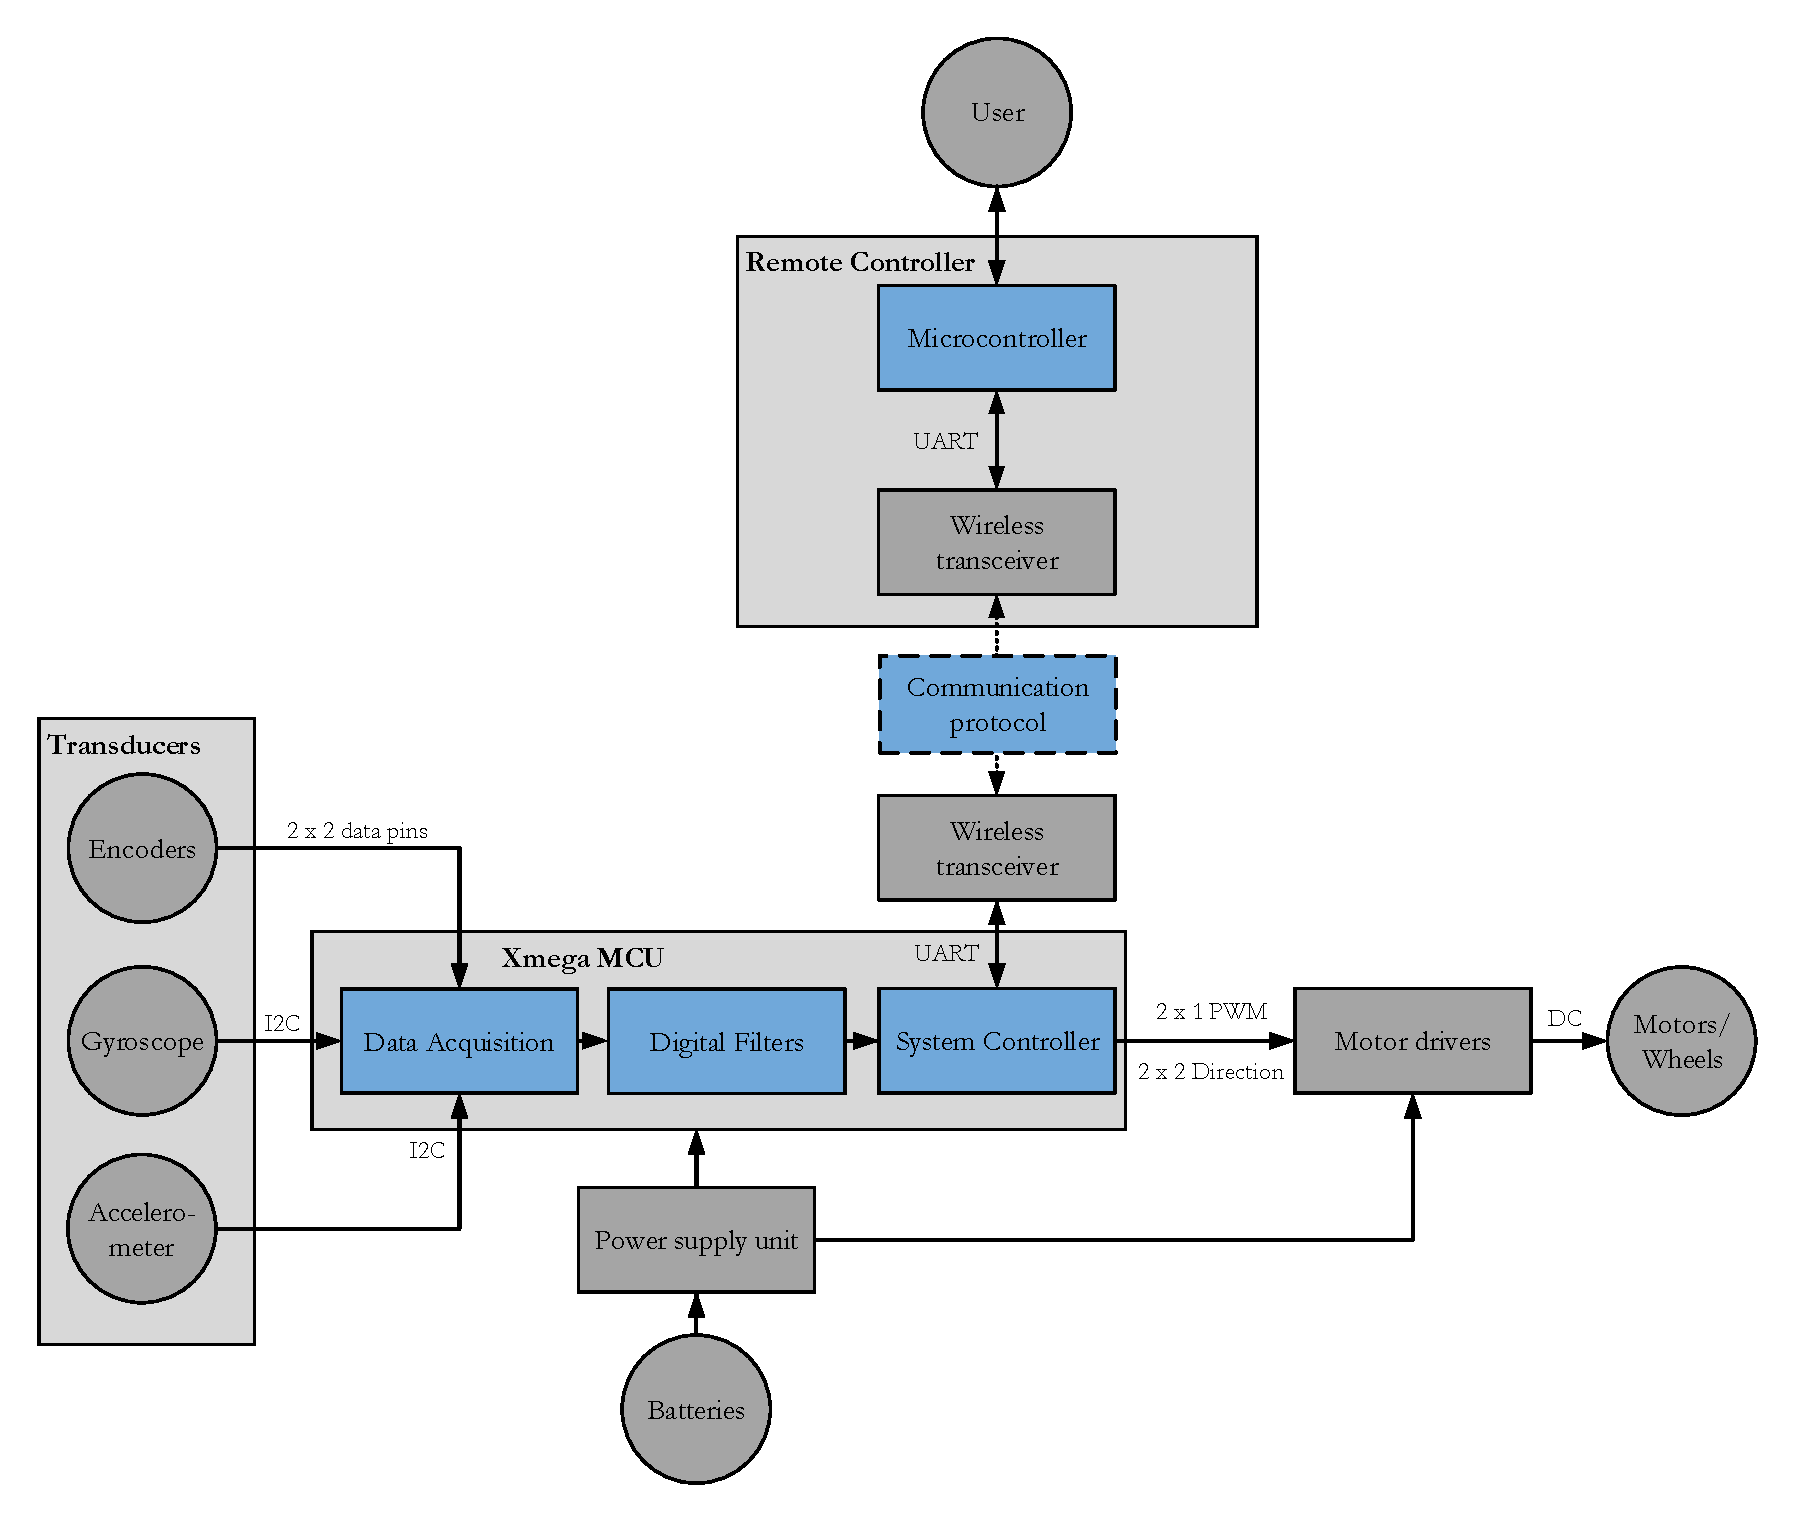
\includegraphics[width=0.95\textwidth]{design/figures/extendedOverviewGrayedWithInterfaces.pdf}
	\caption{Overview of the system. The blue blocks are blocks the design primary deals with.}
	\label{fig:system_overview_block}
\end{figure}
Note that a communication protocol has been inserted between the wireless transceivers. This is done because some "rules" has to be introduced in the communication between the remote controller and the MCU on the segway to ensure a proper data transfer without misunderstandings.

Also, a filter is inserted between the encoders and the MCU. To avoid breaking electrical interfaces and changing the electrical configuration of the segway, the filter is implemented as a digital filter, instead of an analog.

To ensure that subsystems can be designed parallel, the interfaces between subsystems have to be clarified. Data types transmitted between subsystems are shown in \autoref{fig:system_overview_block}. From left, the gyroscope and accelerometer transmits measured values through an $I^{2}C$ communication protocol, and the encoders data through two data pins. For external communication to the remote controller, data is transferred through a UART interface which is supported by both the wireless transceiver and the microcontroller. To control the motor drivers, a PWM signal is used for each motor, together with two direction pins.

\subsection{Control Loop Overview}\label{controlLoopOverview}
The system that controls the balancing of the segway can be described as a closed loop system, as shown in \autoref{fig:segOverview}. The segway is balanced through the use of three subsystems, namely the controller (D), the plant (G) and the sensors (H). It is assumed that the sensors are ideal, meaning that their frequency response is equal to unity i.e. $H(s) = 1$, as this block won't include any amplification or filtering, but solely measure. This is done since it is decided not to determine the sensor's transfer function, and that it will make the calculations easier by assuming that the measued output data is identical to the actual output. The input, R, is the desired angle of the segway, which for the balancing functionality, will be zero, i.e. the steady state upright position. The output $Y$ is the actual angle of the segway, denoted as $\theta_p$.

\begin{figure}[H]
\centering
\input{figures/modelBlockOverview.ralf}
\caption{A feedback loop of the system that controls the balance of the segway.}
\label{fig:segOverview}
\end{figure}

The plant is based on a model of the system that describes the movement of the segway, where the output is $Y = \theta_p$. This model is found in \autoref{ch:modelling}. %The input to the plant model is determined in \autoref{ch:modelling}, where the model is derived from an analysis of the segway. %The plant is used to directly change the output of the closed loop feedback system.

The controller block, D, generates the input to the plant, based on the difference between the desired angle, R, also known as the reference, and the actual angle measured by the sensor system, H. The output of the controller, U, is generated so that the error between output of the plant, Y, and the desired angle is minimized. The design of the controller unit is performed in \autoref{ch:Controller}.

%In the following chapter, the plant model is derived, as this lies the foundation for the controller design.

Now that the segway platform has been described, it is possible to set up the requirements for the system, which is done in the following chapter.



%The interface requirements is needed in order to determine the data type of the inputs and outputs of each subsystem.


%\section{Interface requirements} \todo{The section is still a sketch}
%\todo{reduce section}
%To ensure subsystems can be designed individually it is necessary to define the interface requirements. The interface requirements is needed in order to determine the data type of the inputs and outputs of each subsystem. 
%
%\subsection{Filter}
%
%The input of the filter is an analog signal from the encoders. The signal contains data about the rotation and direction of the motors. Since the inputs from the encoders are analog the best solution, are to make the filter analog as well. \todo{Is the encoder output analog or digital?}
%
%\subsection{Data Acquisition}
%
%As seen on \autoref{fig:system_overview_block} the data acquisition block receives input from the encoders, gyroscope, and accelerometer. Since the microcontroller only operates with digital signals any analog signal from the transducers has to be sampled into digital signal. 
%
%Another task is to convert measured data into understandable data types. This makes it easier to apply the measured data into control algorithm in the system controller.
%
%\subsection{System controller}
%
%Both data acquisition and the wireless transceiver transfers data to the system controller. The input from the data acquisition block is digital data from the transducers. Input from the wireless transceiver is digital as well but the communication protocol has to be the same as on both controllers.
%
%\subsection{Motor controller}
%
%The input of the motor controller is a digital signal from the system controller. The input could be data telling that the segway should move forward. Since the output of the motor controller is connected to the motor driver, it is necessary to insure that data from the motor controller is the same type of the motor driver.
%
%\subsection{Microcontroller for remote controller}
%
%
%
%\subsection{Communication protocol}
%
%
%
%\subsection{User input}
%
%
%
%
%\begin{enumerate}
%\item Modelling
%\item Designing subsystems
%\item System integration
%\item System implementation
%\end{enumerate}





%\chapter{Requirements}
This chapter has the purpose of presenting considerations concerning setting up requirements for the the segway. Firstly, the considerations will be made upon a list of requirements set from the preanalysis as well as common sense, for those requirements which has to be set by choice rather than theory. These considerations will result in a list of specific requirements, from which the modelling and controller design of the segway will be designed upon. \\
The requirement considerations follows in the next section.
\section{Requirements Considerations}
The most important functionality of a segway is for it to keep its balance. For this to be achieved, the segway must be able to obtain a stable position after being given an impulse, such as a push. \\
It is preferable to set requirements for the system's step response, as this is a typical measure for a system's dynamic behaviour that is rather easy to measure and set requirements for. In the following, the system's step response's parameters will be described. Afterwards the relation of the system's stability and the phase margin and gain margin will be presented. 

\subsection{Functional Requirements}
For the system, there are some requirements for the overall functionalities of the system. These requirements are derived from intuition, based on what a segway should be able to do.
This includes that the segway has to stabilize itself and balance in an upright position, as well as being able to drive and turn, without falling over. Also, the segway should be able to withstand a light push, without falling over. A "light push" is not defined further, but the push needs to be so big that it makes the segway move in order to stabilize. 
It is also decided that it should also be possible to remote control the segway wirelessly, by means of making the segway drive and turn. The user should also be able to wirelessly receive information from the segway, such as the pendulum angle, $\theta_p$. 

\subsection{Time Domain Requirements}
The step response displays the time behaviour of the system when given an impulse. \autoref{fig:GIR} shows an example of a step response of a dynamic system.

\begin{figure}[H]
\centering
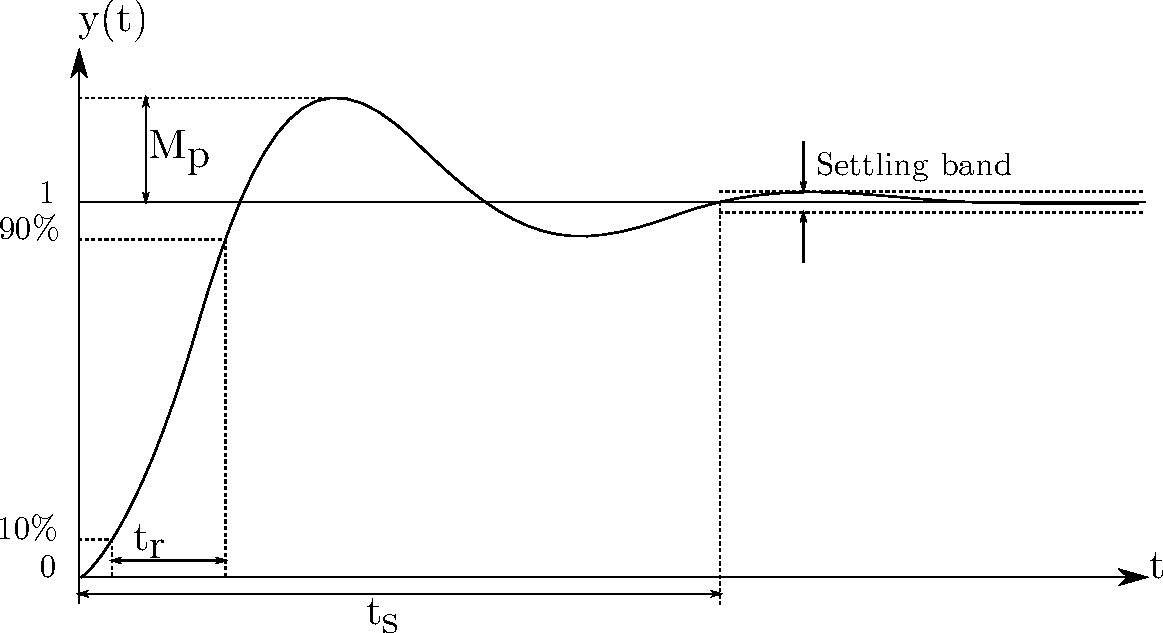
\includegraphics[width = 0.8\textwidth]{figures/steprequ.pdf}
\caption{General step response in time domain. } 
\label{fig:GIR}
\end{figure}
In \autoref{fig:GIR}, the variable $t_r$ is the rise time, defined as the time it takes for the step response to go from 10\% to 90\% of the step. The settling time, $t_s$, describes the time it takes for the system to settle within a certain margin of the final value, typically 1\%, 2\% or 5\%. The steady state error is the difference between the desired steady state value, and the actual steady state value. 
%The variable $t_p$, is the time it takes for the system to reach its maximum value, also called the peak time.
The ratio between the step response's ideal level and the maximum level which the system reaches is the overshoot, $M_p$.\\
To make sure the control system is stable, the system should not have any poles in the right-half-plane of the s-plane \citep[p. 146]{sou:Feedback}, or any poles outside the unit circle, if considering the z-plane \citep[p. 619]{sou:Feedback}.
\\\\
It is desirable not to have a steady-state error, as the balancing of the segway shall be as accurate as possible, to ensure that the angle the segway is to maintain is also met, as an steady-state error in the inverted pendulum angle will cause the segway to move forward or backwards.
It is likewise desirable to have a fast rise time, as it would decrease the risk of the segway of falling over if the controller regulates the segway to an upright balanced position quickly. However, this will result in an overshoot, as the system's quick response to the impulse, for example a push, will make the system overcompensate to minimize the error quickly. This will increase the risk of the segway of falling over, if the overshoot is so high that the segway falls to the other side. The overshoot can also cause oscillations, if the controller constantly tries to obtain the desired angle, but has an overshoot so high, that the overshoot angle also has to be corrected by the controller. Disturbances to the controller making the system unstable, such as the gravity, can affect the way the segway moves forward at a steady velocity. It is important to reduce both disturbances and noise affecting the sensor values, to obtain a control system with high precision.\\
The segway's balance controller shall thus, as with any control system, be a compromise of an agile behaviour, where the settling time is not too long and where overshoot is limited.

The step response is a useful means of evaluating the dynamics of a system, i.e. the rise and settling time, the overshoot and the steady state error. The step is applied to the closed loop, as the step response then includes the effect of the feedback.

The general transfer function for the basic closed loop feedback system is shown in \autoref{eq:GCL} and the corresponding block diagram is shown in \autoref{fig:GCL}. 

\begin{equation}
T(s) = \frac{Y(s)}{R(s)} = \frac{\text{Direct term}}{1 + \text{Open loop}}
\label{eq:GCL}
\end{equation}
%\begin{where}
%\punkt{$T(s)$}{function for closed loop magnitude in s domain}{dB}
%\punkt{$Y(s)$}{function for output signal}{dB}
%\punkt{$R(s)$}{function for input signal}{dB}
%\punkt{$D(s)$}{function for controller}{dB}
%\punkt{$G(s)$}{function for plant}{dB}
%\punkt{$H(s)$}{function for sensor}{dB}
%\end{where}

\begin{figure}[H]
\centering
\input{figures/GeneralClosedLoop.ralf}
\caption{Block diagram of a general closed loop feedback system.}
\label{fig:GCL}
\end{figure}

It is assumed that the system that is to be controlled is a second order stable closed loop system, on the form as listed in \autoref{TFgeneral}.
\begin{equation}
T(s)=\frac{A}{s^2 + 2\zeta\omega_n s + \omega_n^2}
\label{TFgeneral}
\end{equation}
\begin{where}
\va{$A$}{is the DC gain}{1}
\va{$\zeta$}{is the damping factor}{1}
\va{$\omega_n$}{is the natural frequency}{rad/s}
\end{where}

Due to this, the relationship between the different quantities can be expressed from the following rules of thumb \citep[p. 152]{sou:Feedback}:
\begin{align}
M_p &= \exp{\frac{-\pi \zeta}{\sqrt{1-\zeta^2}}} \label{overshoot}\\
t_r &\approx \frac{1.8}{\omega_n}\label{risetime}\\
t_s &= \frac{-\text{ln}(x)}{\zeta\omega_n}, x = \text{settling band, e.g. 0.01 for 1\%} \label{settlingtime}\\
\zeta &\approx \frac{PM}{100}\label{zeta}
\end{align}

Assuming that the system is 2nd order, it is thus possible to set up realistic requirements for the system based on these equations. First of, it is decided that no steady-state error is acceptable, as it will cause the pendulum to move forward at a steady velocity at all times, which is not desired.

It is chosen that the overshoot should be no more than 10\%, i.e. $M_p \leq 0.10$. Using \autoref{overshoot}, $\zeta$ is found to be equal to $\zeta = 0.8$. By deciding that the settling time $t_s$ should be less than 3 seconds for a 1 \% settling band, it is found that $\omega_n = 1.92$ using \autoref{settlingtime} and the found value for $\zeta$.
This can be inserted in \autoref{risetime}, giving a rise time of $t_r = 0.94 \, s$. This is considered acceptable, but to give some margin, the requirement is increased to 1 s. Thus, the requirements for the step response of the system has been determined. The requirements are summed up below.

Steady state error: 0 \%\\
Rise time: < 1 s\\
Settling time: < 3 s\\
Overshoot: $\leq$ 10 \% 

%The exact proportions can not be found from theory or rule of thumb, but instead determined from simulations and tests on a model of the system. The compromise of the three values, namely rise time, settling time and overshoot, will therefore not be determined at this point. There can be set some guidelines, to limit the simulations and tests. These guidelines is build upon rules of thumb and are evaluated and chosen by the projectgroup. \todo[inline]{not finnished, look besides it!}




%If the rise time is very large, the segway will not be able to stabilise itself before hitting the ground. The rise time is not the only variable in this matter. 
%The force applied by the push can be too large for the mini segway to arise from. The rise time neither be too short, as this would increase overshoot. By having a too large overshoot, the mini segway is more likely to fall if first pushed in one direction, then, as the mini segway enters overshoot, starts driving in the same direction.
%Thus the rise time should be determined as compromise between these two reasons.
%The overshoot should be as small as possible, since overshoot increases the risk of the mini segway to fall, when the mini segway is driving at changing speeds.
%The shorter the settling time and steady state error, the faster the segway stabilises itself at its upright position. Thus these variables should be as short as possible.

With requirements set up for the time domain response of the signal, it is now desired to set up requirements for the frequency domain. This is done by means of requirements to the phase and gain margin. 

%From the step response, the transfer function of the system can be found. The transfer function gives the phase and gain margin if plotted in a bodeplot. 

\subsection{Frequency Domain Requirements}
Phase margin (PM) and gain margin (GM) are two correlating values that describes how far the system is from instability, i.e. how much uncertainty can be allowed before it may cause the system to become unstable \citep{sou:pM}.
For this reason, the requirements for the segway should take these margins into account. %Firstly however, it is necessary to describe what makes for an unstable feedback system. This is done in the following text, with a starting point in general closed loop feedback systems. 

The closed loop feedback system will be unstable if the signal that is fed back from the output to the controller, see \autoref{fig:GCL}, reinforces the error signal, E rather than diminishing it. This is the case if the open loop term is negative, i.e. the signal is phase shifted more than $-180\degree$ at unity gain.

Thus, through analysis of the open loop, it can be determined if the closed loop will be stable. The analysis is performed by determining the PM and GM. This can be done through bode plots of the open loop, as shown in \autoref{fig:phaseGain} and described in the following.

\begin{figure}[H]
\centering
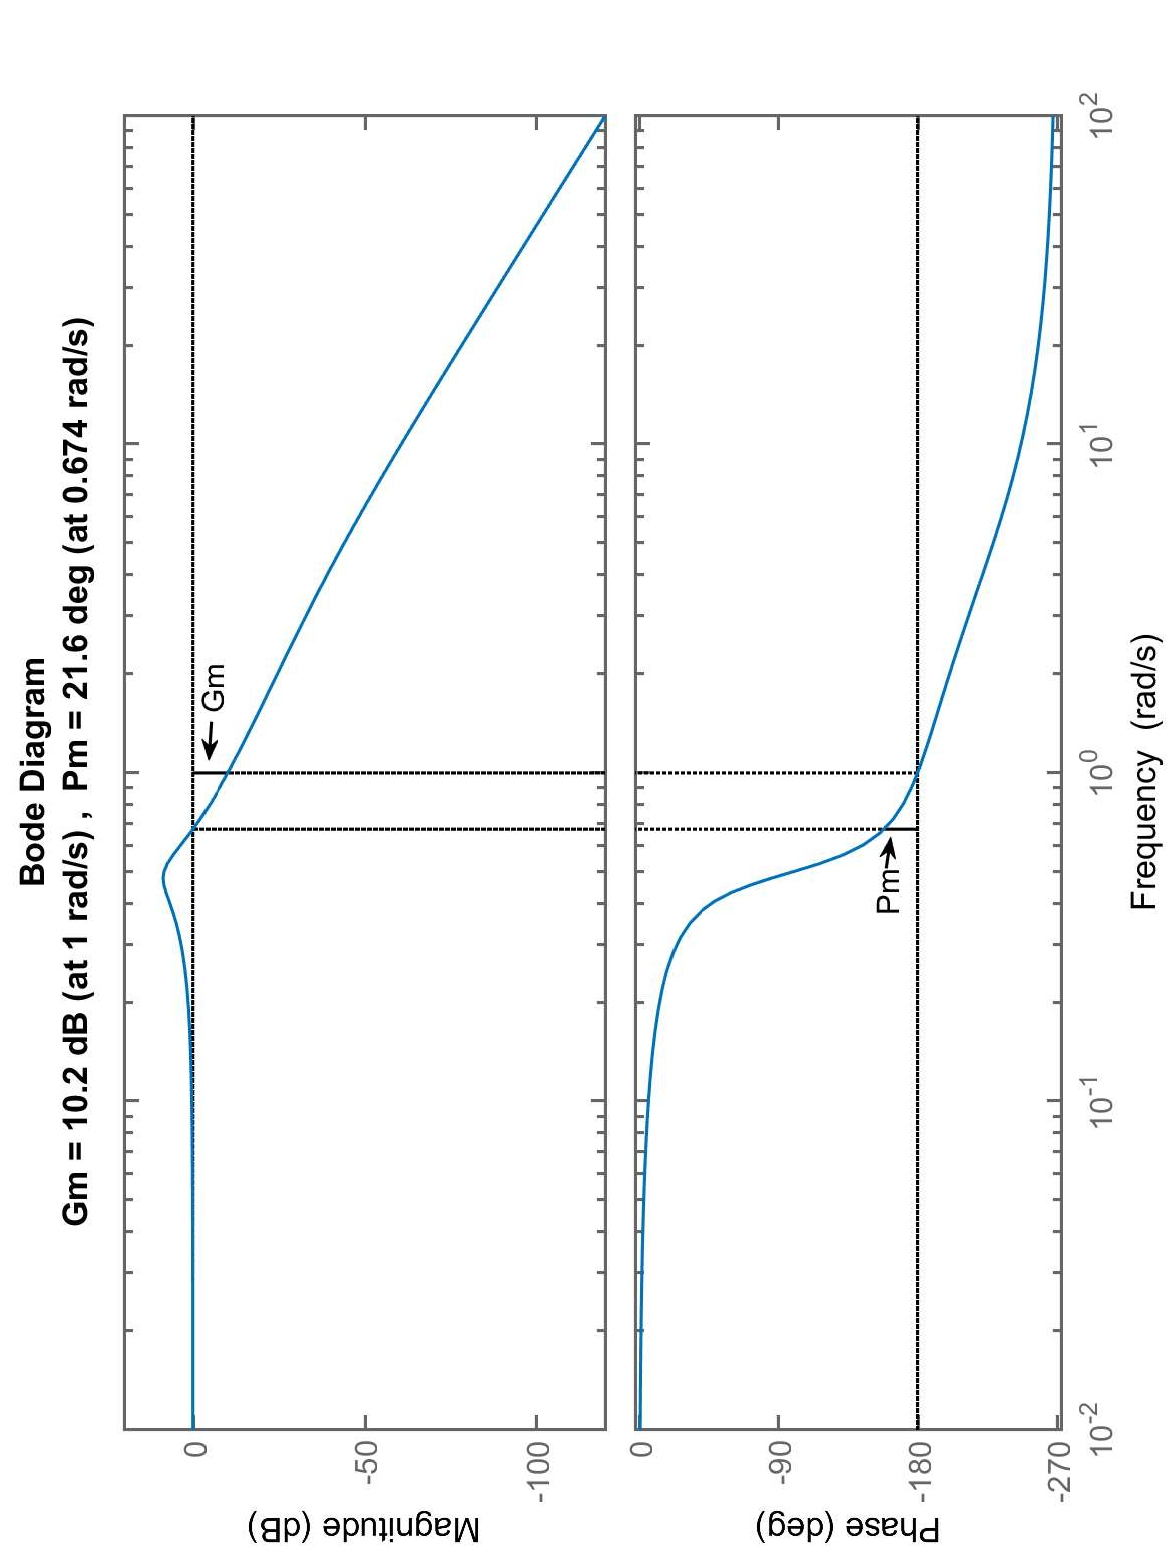
\includegraphics[width=0.6\textwidth, angle=-90]{figures/PM_GM.pdf}
\caption{Bodeplots of an open loop illustrating PM and GM.}
\label{fig:phaseGain}
\end{figure}
The phase margin is found by reading the angle velocity from the magnitude bode plot at gain = 0 dB, and finding the phase angle at this anglular velocity on the phase angle plot. The phase angle subtracted from $-180\degree$ yields the PM \citep{sou:MC}.

The gain margin is found by reading the angular velocity from the phase angle plot at the phase of $-180\degree$, and finding the gain at this angular velocity on the magnitude plot. The difference between this gain and unity gain (0 dB) is the gain margin.

From \autoref{fig:phaseGain}, it can be concluded that the phase margin is defined as how much additional phase shift it would take before the system becomes unstable. On the other hand, the gain margin describes how much the gain may change before the system becomes unstable.

In the beginning of this section, it was stated that the purpose with PM and GM is to keep uncertainties from making the system unstable. In this context, uncertainties being everything that causes the closed loop system to not behave ideally, such as circuit component sensitivity, delay caused by sampling etc. The scale of these inconsistencies is not yet know, so the exact influence these will have on the system cannot be determined. A rule of thumb regarding the PM and GM, states that PM should be greater than or equal to $45\degree$ whereas GM should be greater than or equal to 6 dB \citep{sou:PmGm}. However, to fulfill the time domain requirements, it is necessary to have $\zeta \geq 0.8$, which, based in \autoref{zeta}, results in a phase margin requirement of at least $80 \degree$.\\
From the above considerations, a list of specific requirements can now be set.

\section{List of Requirements \label{requirements}}
Based upon the previous considerations, requirements for the segway can be determined. The requirements are as follows:

\subsection*{Functional Requirements}
\begin{enumerate}
\item The segway must be able to stabilise itself in an upright equilibrium state.\label{funcReqBalance}
\item The segway must be able to drive forward and backwards without causing the segway to fall over.
\item The segway must be able to turn without causing the segway to fall over.
\item The segway may not fall over when pushed lightly.
\item The user must be able to make the segway drive by a wireless controller.
\item The user must be able to make the segway turn by a wireless controller.
\item The user must be able to receive data from the segway on a wireless controller.
\end{enumerate}
\subsection*{Performance Requirements}
The following requirements describes the desired performance of the segway. The first list of requirements is for the time domain, determining the dynamic behaviour of the segway. %Note that these requirements are made based on choices made by the project group and therefore chosen.
\begin{itemize}
\item Steady state error: 0 \%
\item Rise time: $\leq$ 1 s
\item Settling time: $\leq$ 3 s
\item Overshoot: $\leq$ 10 \% 
\end{itemize}
The following list describes the desired stability margins, i.e. the frequency domain requirements:
\begin{itemize}
\item Phase margin: $\geq 80\degree$
\item Gain margin: $\geq$ 6 dB
\end{itemize}

Now that the requirements are set, the development of the system can begin. This includes designing the controller which is to stabilize the system, together with a filter design and the design of the remote controller and the communication protocol. In the following section, a model of the system is derived, as this is needed to make a controller for the system.
%\begin{itemize}
%\item Rise time: TBD
%\item Settling time: TBD
%\item Overshoot: TBD
%\item Steady state error: TBD
%\item 
%
%\end{itemize}



%\section{Acceptance test description}
%Another title.\\

%\subsection{Performance requirements}
%Based on these principles requirements will be set as follows:
%\begin{enumerate}
%\item 
%\end{enumerate}
%
%\begin{enumerate}
%	\item Segway must be able to balance
%	\begin{itemize}
%		\item Rise time
%		\item Settling time
%		\item (Overshoot)
%		\item Phase margin - rule of thumb
%		\item Gain margin - rule of thumb
%	\end{itemize}
%	\item Segway must be able to drive
%	\begin{itemize}
%		\item Forward/Backward
%		\item Turning
%	\end{itemize}
%	\item It must be possible to remote control the segway wirelessly
%	\begin{itemize}
%		\item Zigbee
%		\item remote control drive elements
%	\end{itemize}
%	
%\end{enumerate}
%\chapter{Sensors}
In this chapter, the setup of the sensors used by the segway is described. In a control system the sensors measure the output of the system, $Y$, and feed it back into the system as seen in \autoref{fig:modelBlockS}.

\begin{figure}[H]
\centering
\scalebox{0.8}{
\input{figures/modelBlock.poul}
}
\caption{Feedback loop of a system, with the sensor, $H$, highlighted.}
\label{fig:modelBlockS}
\end{figure}
A general feedback loop, see \autoref{fig:modelBlockS}, consists of three blocks. A controller, $D$, the system that is to be controlled, known as the plant, $G$, and sensors, $H$. The loop holds a reference signal, $R$, an error signal, $E$, the control signal, $U$, between the controller and the plant, and an output, $Y$. It is the sensor block, that is to be determined in this chapter, as highlighted in \autoref{fig:modelBlockS}.

In Section \ref{controlLoopOverview}, it was argued why the transfer function of the sensor block was set to be equal to 1, i.e. $H(s)=1$. Even though this is the case, the sensors used in the system still need to be described, so it is known which parameters of the system are measurable. This is also important to investigate since the way the data is obtained might influence the implementation of the controller.

The segway has four sensors that can be used to measure the speed, angular velocity and angle of the segway. To measure the speed, two encoders are available to measure the rotational velocity for both motors. The angle and angular velocity can be found from the gyroscope and the accelerometer. The structure of the following sections is to first describe the interface between the sensor hardware and the microcontroller (MCU) ATxmega128A3U and afterwards explain the implementation. %How the data is preprocessed is also described. The implementation is done on a ATxmega128A3U microprocessor. 

\section{Accelerometer and Gyroscope}
From \autoref{sec:hardware} it is known that the accelerometer and gyroscope are part of the MPU6050 transducer. This sensor has six degrees of motion, since both the accelerometer and gyroscope are 3-axis sensors. The accelerometer and gyroscope are used to derive the angle and angular velocity of the segway. To acquire the measured data from the sensors, the sensors have an \gls{I2C} bus, which can be interfaced to from the MCU.
  
\subsection{\iic Data}
The physical interface consists of two wires Serial Data (SDA) and Serial Clock (SCL). In normal mode the bus supports clock speeds up to 400 kHz, but additions can be made so the speed can go up to 5 MHz \citep{I2C}. In idle the voltage on the data line is pulled high. On a data level, a transmission consists of a start sequence, 7 bit address, R/W bit, acknowledge, followed by a start sequence, 8 data bit, acknowledge and a stop sequence. This can also be seen in \autoref{fig:I2CFrame}. Note that it is possible to transmit multiple data bytes without having to specify the address between each data transfer.

\begin{figure}[H]
\centering
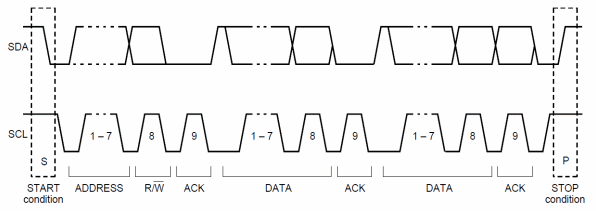
\includegraphics[width=\textwidth]{I2Cframe.png}
\caption{A visual representaion of a \gls{I2C} frame \citep{sou:i2c}.}
\label{fig:I2CFrame}
\end{figure}

\subsection{Data Acquisition from Gyroscope and Accelerometer}
The \gls{I2C} communication protocol is implemented in the MCU as a software module, since the pins, connected to pin 0 and 1 on port A, do not support hardware \gls{I2C}. The implemented \gls{I2C} driver, has been provided by group 15gr633, from AAU, who previously worked with the segway. From the header file, it can be seen that the library has 11 functions \autoref{lst:I2CFunctions}. From these functions the three functions i2cInit, i2cWrite and i2cRead are the main functions, the rest are subroutines that are called from the main functions.

\lstset{language=C, caption={Pre initialization of \gls{I2C} functions.}, label=lst:I2CFunctions}
\begin{lstlisting}
void i2cInit();
uint8_t i2cWrite(uint8_t slaveAddr, uint8_t regAddr, uint8_t *data, uint8_t length);
uint8_t i2cRead(uint8_t slaveAddr, uint8_t regAddr, int8_t *data, uint8_t length);

void i2cRepeatedStart(); 
void i2cStart();
void i2cStop();
void i2cTransmit(uint8_t data);
uint8_t i2cReceive();
uint8_t i2cGetAck();
uint8_t i2cSendAck();
uint8_t i2cSendNack();
\end{lstlisting}

From the datasheet it is known that the MPU6050 sensors \gls{I2C} address is 0x68 \citep[p. 46]{gyro}. When the sensor is powered on, it is in sleep mode. To wake up the sensor, 0x00 is written to the PWR\_MGMT\_1(Power Management 1) 8-bit register. Each sensor has six 8-bit registers for measured data. The three axes' values are sampled by three 16-bit ADC and then stored as MSB and LSB, giving six data registers for each sensor. From the datasheet it is known that the accelerometer data is stored in the registers from 0x3B to 0x40, while the gyroscope data is stored in the registers from 0x43 to 0x48. 

Note that both the gyroscope and the accelerometer work in polling mode, meaning that the current measurements are not sent automatically to the microcontroller, but will instead have to be requested over \gls{I2C}. The sensor modules takes care of obtaining the measurements and storing them in an internal register automatically - it is only the extraction of this data that is done in polling mode.

\subsection{Data Processing the Gyroscope and Accelerometer}
When the data is collected from the registers, they are put together to three 16 bit words. The accelerometer and gyroscope use the same coordinate system, but the orientation of this coordinate system (x, y, z) must be compared to the segway, which can be seen in \autoref{fig:sensor_orientation}. 

\begin{figure}[H]
\centering
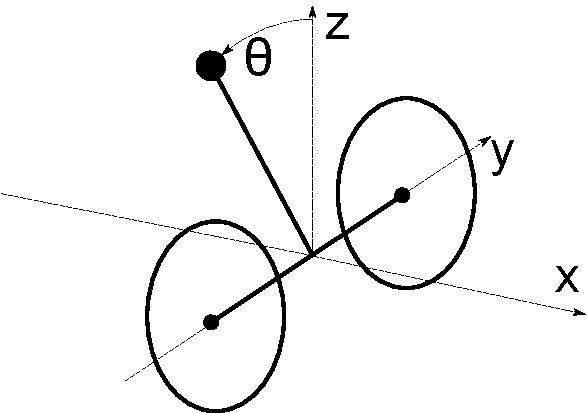
\includegraphics[width=0.4\textwidth]{figures/3D_seg_balance.pdf}
\caption{The sensors' orientation compared to the segway.}
\label{fig:sensor_orientation}
\end{figure}

To calculate the tilting angle of the pendulum, $\theta_p$, different methods can be used. For instance, the accelerometer can calculate the angle based on the direction of gravity, or by integrating the gyroscope data, which measures angular velocity. These methods have a couple of problems though. For instance, the accelerometer is very sensitive to changes in movement due to the acceleration applied. The gyroscope however, has a tendency to drift due to the integration \citep{IMU}. To obtain the angle it can therefore be advantageous to combine these measurements. This is done in a complementary filter \citep{IMU}, where measurements from both of the sensors are weighted and summed. 
\newpage
From \autoref{fig:sensor_orientation} it can be deducted that the pendulum angle can be calculated based on the accelerometer as: 
$$\theta_{pAx} = -\text{tan}^{-1}\left(\frac{x_{Ax}}{z_{Ax}}\right)$$ 
\begin{where}
\va{$\theta_{pAx}$}{is the angle of pendulum}{$\text{rad}$}\\
\va{$x_{Ax}$}{is the accelerometer measurement in the x-axis}{1}\\
\va{$z_{Ax}$}{is the accelerometer measurement in the z-axis}{1}\\
\end{where}

To get the angular velocity from the gyroscope, it is first recognised, based in \autoref{fig:sensor_orientation}, that it is the data in the y-axis, that is of interest. 
The angular velocity can then be calculated as follows:
\begin{equation}
\omega_p = \frac{y_{Gyro} \cdot max}{n}
\end{equation}
\begin{where}
	\va{$\omega_p$}{is the angular velocity of the pendulum}{rad/s}
	\va{$y_{Gyro}$}{is the data from the gyroscope in the y-axis}{1}
	\va{$max$}{is the gyroscope maximum measurement}{rad/s}
	\va{$n$}{is the number of digital representation for the gyroscope data}{1}
\end{where}

Using the complementary filter, the angle can be found as:

\begin{equation}
\theta_p = k \cdot \theta_{pAx} + (1-k) \cdot \int \!\omega_p \,\rm{d}x
\label{complementary}
\end{equation}

From \autoref{complementary}, it is seen how the angle is estimated from both accelerometer and integrated gyroscope data, and then the two values are weighted. The weighting factor $k$ is found experimentally to 0.05.
\newpage
\section{Encoder and Quadrature Decoder}

To determine the velocity of the wheels at a specified time, the exact change of position over an infinitesimal timespan shall be known, as the velocity $v(t)$ can be expressed by the time derivative of the position $s(t)$:
\begin{align}
v(t) = \frac{\text{d}s(t)}{\text{d}t}
\label{velocity}
\end{align}
\begin{where}
\va{$v(t)$}{is a function for velocity}{$\text{m/s}$}\\
\va{$s(t)$}{is a function for position}{$\text{m}$}\\
\end{where}

To determine a function for the position it is desired to decode the output signal from the encoders since they provide measurements about position changes over time. 

The encoders used for the segway are quadrature encoders. The output from a quadrature encoder is two square waves phase shifted by 90$\degree$ from two channels as illustrated in \autoref{fig:incremental_encoders2}. 

\begin{figure}[H]
	\centering
	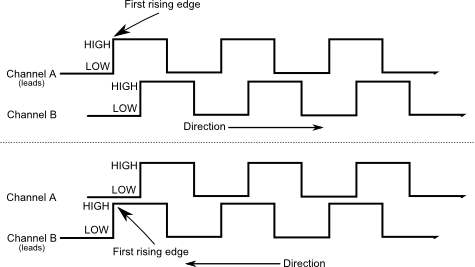
\includegraphics[width=0.7\textwidth]{figures/quad-encoding-waveform.png}
	\caption{Quadrature signal \citep{sou:quad_enc}.}
	\label{fig:incremental_encoders2}
\end{figure}

The signals from the encoders provide information about the direction and velocity of the wheel. Since the square waves from channel A and B are 90$\degree$ out of phase, the direction of the wheels can be found by determining the first rising edge of the signals from channel A and B. As the direction of the wheels change, the first rising edge will occur at the other channel.

The velocity can be determined by the number of of the square waves per time unit. One encoder rotation correspond to 512 high/low cycles or 2048 counts. A count is an event change in either channel A or B. E.g. if channel A goes low it will result in a count. The relation between the position and the number of counts is given by:

\begin{align}
s(t) = \frac{d \cdot \pi \cdot N_{ms} \cdot N_{sw}}{4\cdot CPR} \cdot c(t) \qquad \{c(t) \in \mathbb{Z}\}
\end{align}
\begin{where}
\va{$d$}{is the diameter of the wheel}{$\text{m}$}\\
\va{$N_{ms}$}{is the encoder/shaft ratio}{1}
\va{$N_{sw}$}{is the shaft/wheel ratio}{1}
\va{$c(t)$}{is number of counts. $c(t)$ can only be an integer.}{1}
\va{$CPR$}{number of cycles in one encoder rotation}{1}
\end{where}

The function $c(t)$ changes by the velocity of the wheels. Since $c(t)$ is an integer, the resolution of the position change is limited to the a-coefficient in the equation of $s(t)$, which is a linear expression on the form $s(t) = a \cdot c(t)$. The a-coefficient can be calculated by inserting the values given by the datasheets and measurements, see \autoref{app:segwayParameters} and \autoref{motorMeasReport}.
\begin{align}
s(t) = \frac{d \pi \cdot N_{ms} \cdot N_{sw}}{4\cdot CPR} \cdot c(t) \Rightarrow s(t) = \frac{0.117 \, \text{m} \cdot \pi \cdot  \frac{1}{19} \cdot \frac{25}{90}}{4\cdot 512} \cdot c(t) \approx 2.62 \cdot 10^{-6} \: \text{m} \cdot c(t)
\label{eq_st}
\end{align}

\autoref{eq_st} yields that 1 count is equal to $2.62 \cdot 10^{-6} \: \text{m}$. The expression of $s(t)$ from \autoref{eq_st} is inserted into \autoref{velocity}, yielding:
\begin{align}
v(t) = 2.62 \cdot 10^{-6} \: \text{m} \cdot \frac{\text{d}c(t)}{\text{d}t} \qquad \{c(t) \in \mathbb{Z}\}
\label{eq_vel}
\end{align}

Since the microcontroller responsible for measuring the encoder only works in discrete time, it is impossible to compute the derivative in \autoref{eq_vel}. Instead, a close approximation of \autoref{eq_vel} can be described as:
\begin{align}
v(t) \approx 2.62 \cdot 10^{-6} \: \text{m} \cdot \frac{c(t)-c(t_1)}{t-t_1} = 2.62 \cdot 10^{-6} \: \text{m} \cdot \frac{\Delta c(t)}{\Delta t}
\label{eq_vel2}
\end{align}

Whereas \autoref{eq_vel} gives the exact velocity of the wheels at a given time $t$, \autoref{eq_vel2} gives the approximated velocity in the time span $\Delta t$. This means the precision of the velocity is determined by $\Delta t$. A smaller time span $\Delta t$ gives a better precision.
If the time span $\Delta t$ is fixed, meaning $\Delta t$ is always set to 1 ms, the time span can known as the sampling period $T_{s}$. The inverse of $T_{s}$ is the sampling frequency $f_{s}$.
\begin{align}
v(t) \approx 2.62 \cdot 10^{-6} \: \text{m} \cdot f_s \cdot \Delta c(t) 
\end{align}

To get an accurate velocity, the sampling frequency is set to 1 kHz, but due to rounding in the frequency scaling in the MCU, this frequency cannot be obtained exactly. This small error is however disregarded.
\begin{align}
v(t) \approx 2.62 \cdot 10^{-6} \: \text{m} \cdot 1 \: \text{kHz} \cdot \Delta c(t)  = 2.62 \cdot 10^{-3} \: \frac{\text{m}}{\text{s}} \cdot \Delta c(t) 
\label{eq_vel3}
\end{align}

From this, the wheel angular velocity can also be found:
\begin{align}
\omega_w(t) = \frac{2\pi}{r_w}\cdot v(t) = 963 \cdot 10^{-6} \cdot \Delta c(t) \frac{\text{rad}}{\text{s}}
\end{align}	
The next step is to implement \autoref{eq_vel3} on the microcontroller.

\subsection{Quadrature Decoder Setup}
To process the data from the encoders, some decoders are needed. As stated previously, every event equals to a logical change from channel A or B from the encoders. Since the segway features two encoders, one encoder is connected to port C and another to port E. To allow event detection on the XMEGA, the registers associated with the quadrature decoding are set. The functions used for the setup of the quadrature decoders are seen in \autoref{lst:encoderFunctions}.

\lstset{language=C, caption={Pre-initialization of quadrature decoder functions.}, label=lst:encoderFunctions}
\begin{lstlisting}
void qdec_setup();			// Setup registers for the quadrature decoder
void en_interrupt();		// Enable interrupt
float motor_speed_left();	// Calculate and return the velocity of the left wheel
float motor_speed_right();
\end{lstlisting}

All registers associated with the quadrature decoders are set in the function qdec\_setup(), where the hardware for the decoder is set up. The XMEGA has external hardware that supports quadrature decoding. This means that the microprocessor does not directly need to handle the encoder itself, but only needs to read the data from the decoder through an interrupt service routine (ISR). After calling this function, a counter register will increment by one every time an event changes is occurring from channel A and B from both encoders. 

\subsection{Data Processing the Encoder Measurements}
As previously stated, the sampling frequency for the decoders are set to $f_s = 1$ kHz. To ensure a sampling every 1 ms, a timer is set to count up 1 ms and interrupts in order to sample the counter from the decoders. The interrupt service routine is seen in \autoref{lst:decoderISR}.

\lstset{language=C, caption={Interrupt Service Routine (ISR) for sampling the counters.}, label=lst:decoderISR}
\begin{lstlisting}
ISR(TCD1_OVF_vect){
	encoder_ccnt = TCC1.CNT;		// Get the value from port C counter register
	encoder_ecnt = TCE1.CNT;		// -||- port E
	TCE1.CNT = 0;					// Reset the counter register
	TCC1.CNT = 0;									
}
\end{lstlisting}
If the velocity of the wheels is required, the functions motor\_speed\_left() and motor\_speed\_right() are called. The functions then return the speed of the left and right wheel. This is done by converting the encoder counter to velocity using \autoref{eq_vel3}.
%\begin{equation}
%	\omega_w = 2 \cdot \pi \cdot f_s \cdot N_{ms} \cdot N_{sw} \cdot \frac{cnt}{4 \cdot res}
%\end{equation}
%\begin{where}
%\va{$\omega_w$}{is the angular velocity of the wheel}{rad/s}\\
%\va{$f_s$}{is the sampling frequency of the encoders}{Hz}\\
%\va{$N_{ms}$}{is the gearing ratio from the motor to the shaft}{1}\\
%\va{$N_{sw}$}{is the gearing ratio from the shaft to the wheel}{1}\\
%\va{cnt}{is the counted value for the specific encoder}{1/RPM}\\
%\va{res}{is the resolution of the encoders}{1/RPM}
%\end{where}

\section{PWM and H-bridge}
To control the DC-motors connected to the wheels, two H-bridges are used. By using H-bridges it is possible to control both the direction and the speed of the DC motors. For each H-bridge, the pins D2, IN1 and IN2 on the H-bridge are used for this purpose. By feeding D2 with a PWM signal, the velocity is changed by changing the duty cycle. A duty cycle of 100\% results in the motors going on full speed, whereas a duty cycle of 0\% results in no rotation. To determine the direction, either IN1 or IN2 should be pulled high. \\\\
The H-bridges' IN1 and IN2 pins are connected to the microcontroller's pin PC2 and PC3, and PE2 and PE3. The D2 pin is connected to PC1 and PE1 - these pins are set to be the PWM generating outputs in the MCU. The functions associated with PWM generation can be seen in \autoref{lst:pwmFunctions}.

\lstset{language=C, caption={Pre initialization of PWM generation functions.}, label=lst:pwmFunctions}
\begin{lstlisting}
void PWM_setup();
void PWM_left(int duty);
void PWM_right(int duty);
\end{lstlisting}

When generating a PWM signal, the resolution of the PWM signals are set to 256 counts, which is considered to be sufficient.\\
As the sensor block in the feedback loop, see \autoref{fig:modelBlockS}, is now known, the system model of the segway is to be derived in the following chapter. 


%\section{Controllers}

\chapter{Introduction}

The inverted pendulum is a classical control system, aiming at getting a pendulum with its center of mass above the pivot point to balance, see \autoref{invertedPendulum}. The pendulum consists of a mass $m_p$ on a rod with length $l$, located on a moving base. A force $F_F$ is applied to the base, so the tilting angle of the pendulum, $\theta_p$, is minimized. 

Whereas a regular pendulum is a stable system with an equilibrium point, the inverted pendulum is inherently unstable. This means that unless some action is taken, the pendulum will fall over. To keep the pendulum balanced, it is necessary to measure the tilting angle $
\theta_p$, and, based on a model of the system, make the base move in the correct way by means of an applied force $F_F$.

%\begin{figure}[H]
%\centering
%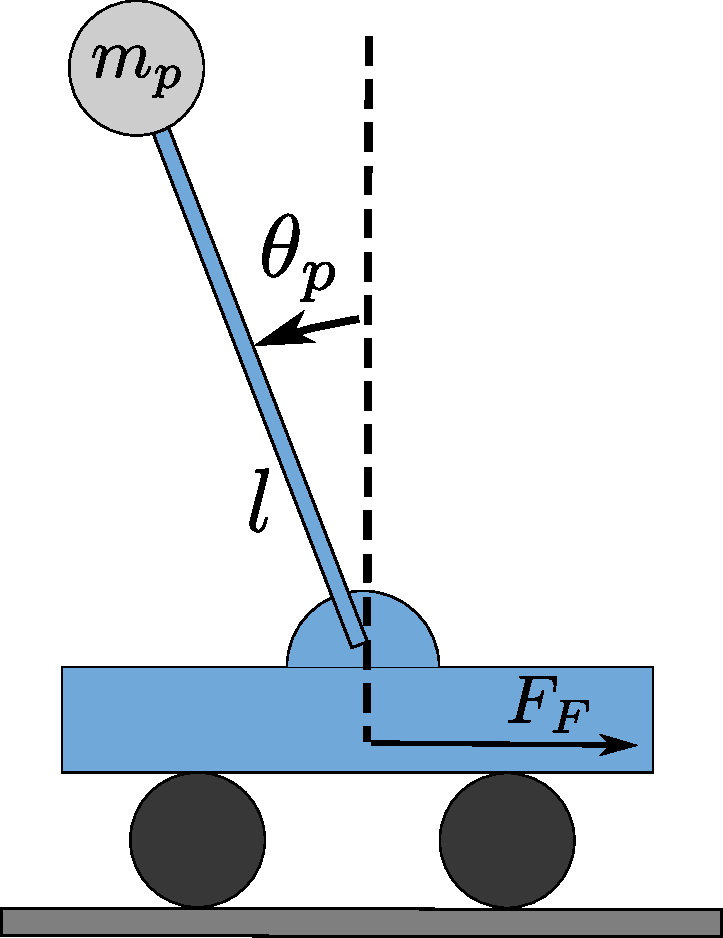
\includegraphics[width=0.4\textwidth]{figures/invertedPendulum.pdf}
%\caption{An inverted pendulum with mass \emph{m} placed on a moving base which is affected by a force $F$. The pendulum has length \emph{l}, and is currently tilted at an angle \emph{$\theta$}}
%\label{fig:invertedPendulum}
%\end{figure}

\begin{figure}[H]
\centering
	\begin{minipage}{0.45\textwidth}

	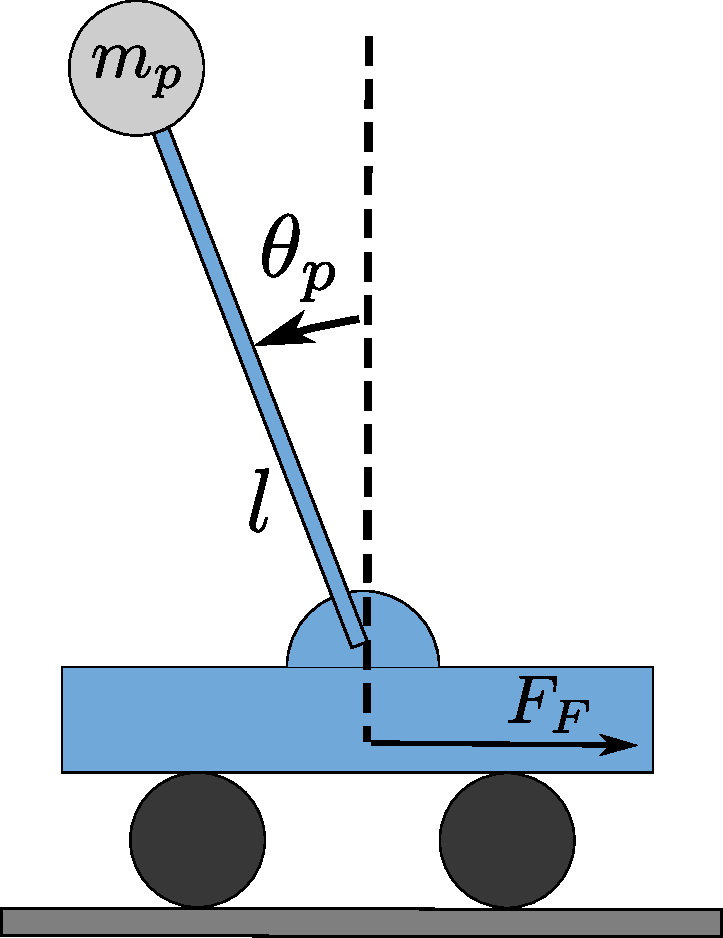
\includegraphics[width=0.9\textwidth]{figures/invertedPendulum.pdf}
	\caption{An inverted pendulum placed on a moving base}
	\label{invertedPendulum}
	\end{minipage}
	\hspace{0.08\textwidth}
	\begin{minipage}{0.40\textwidth}
	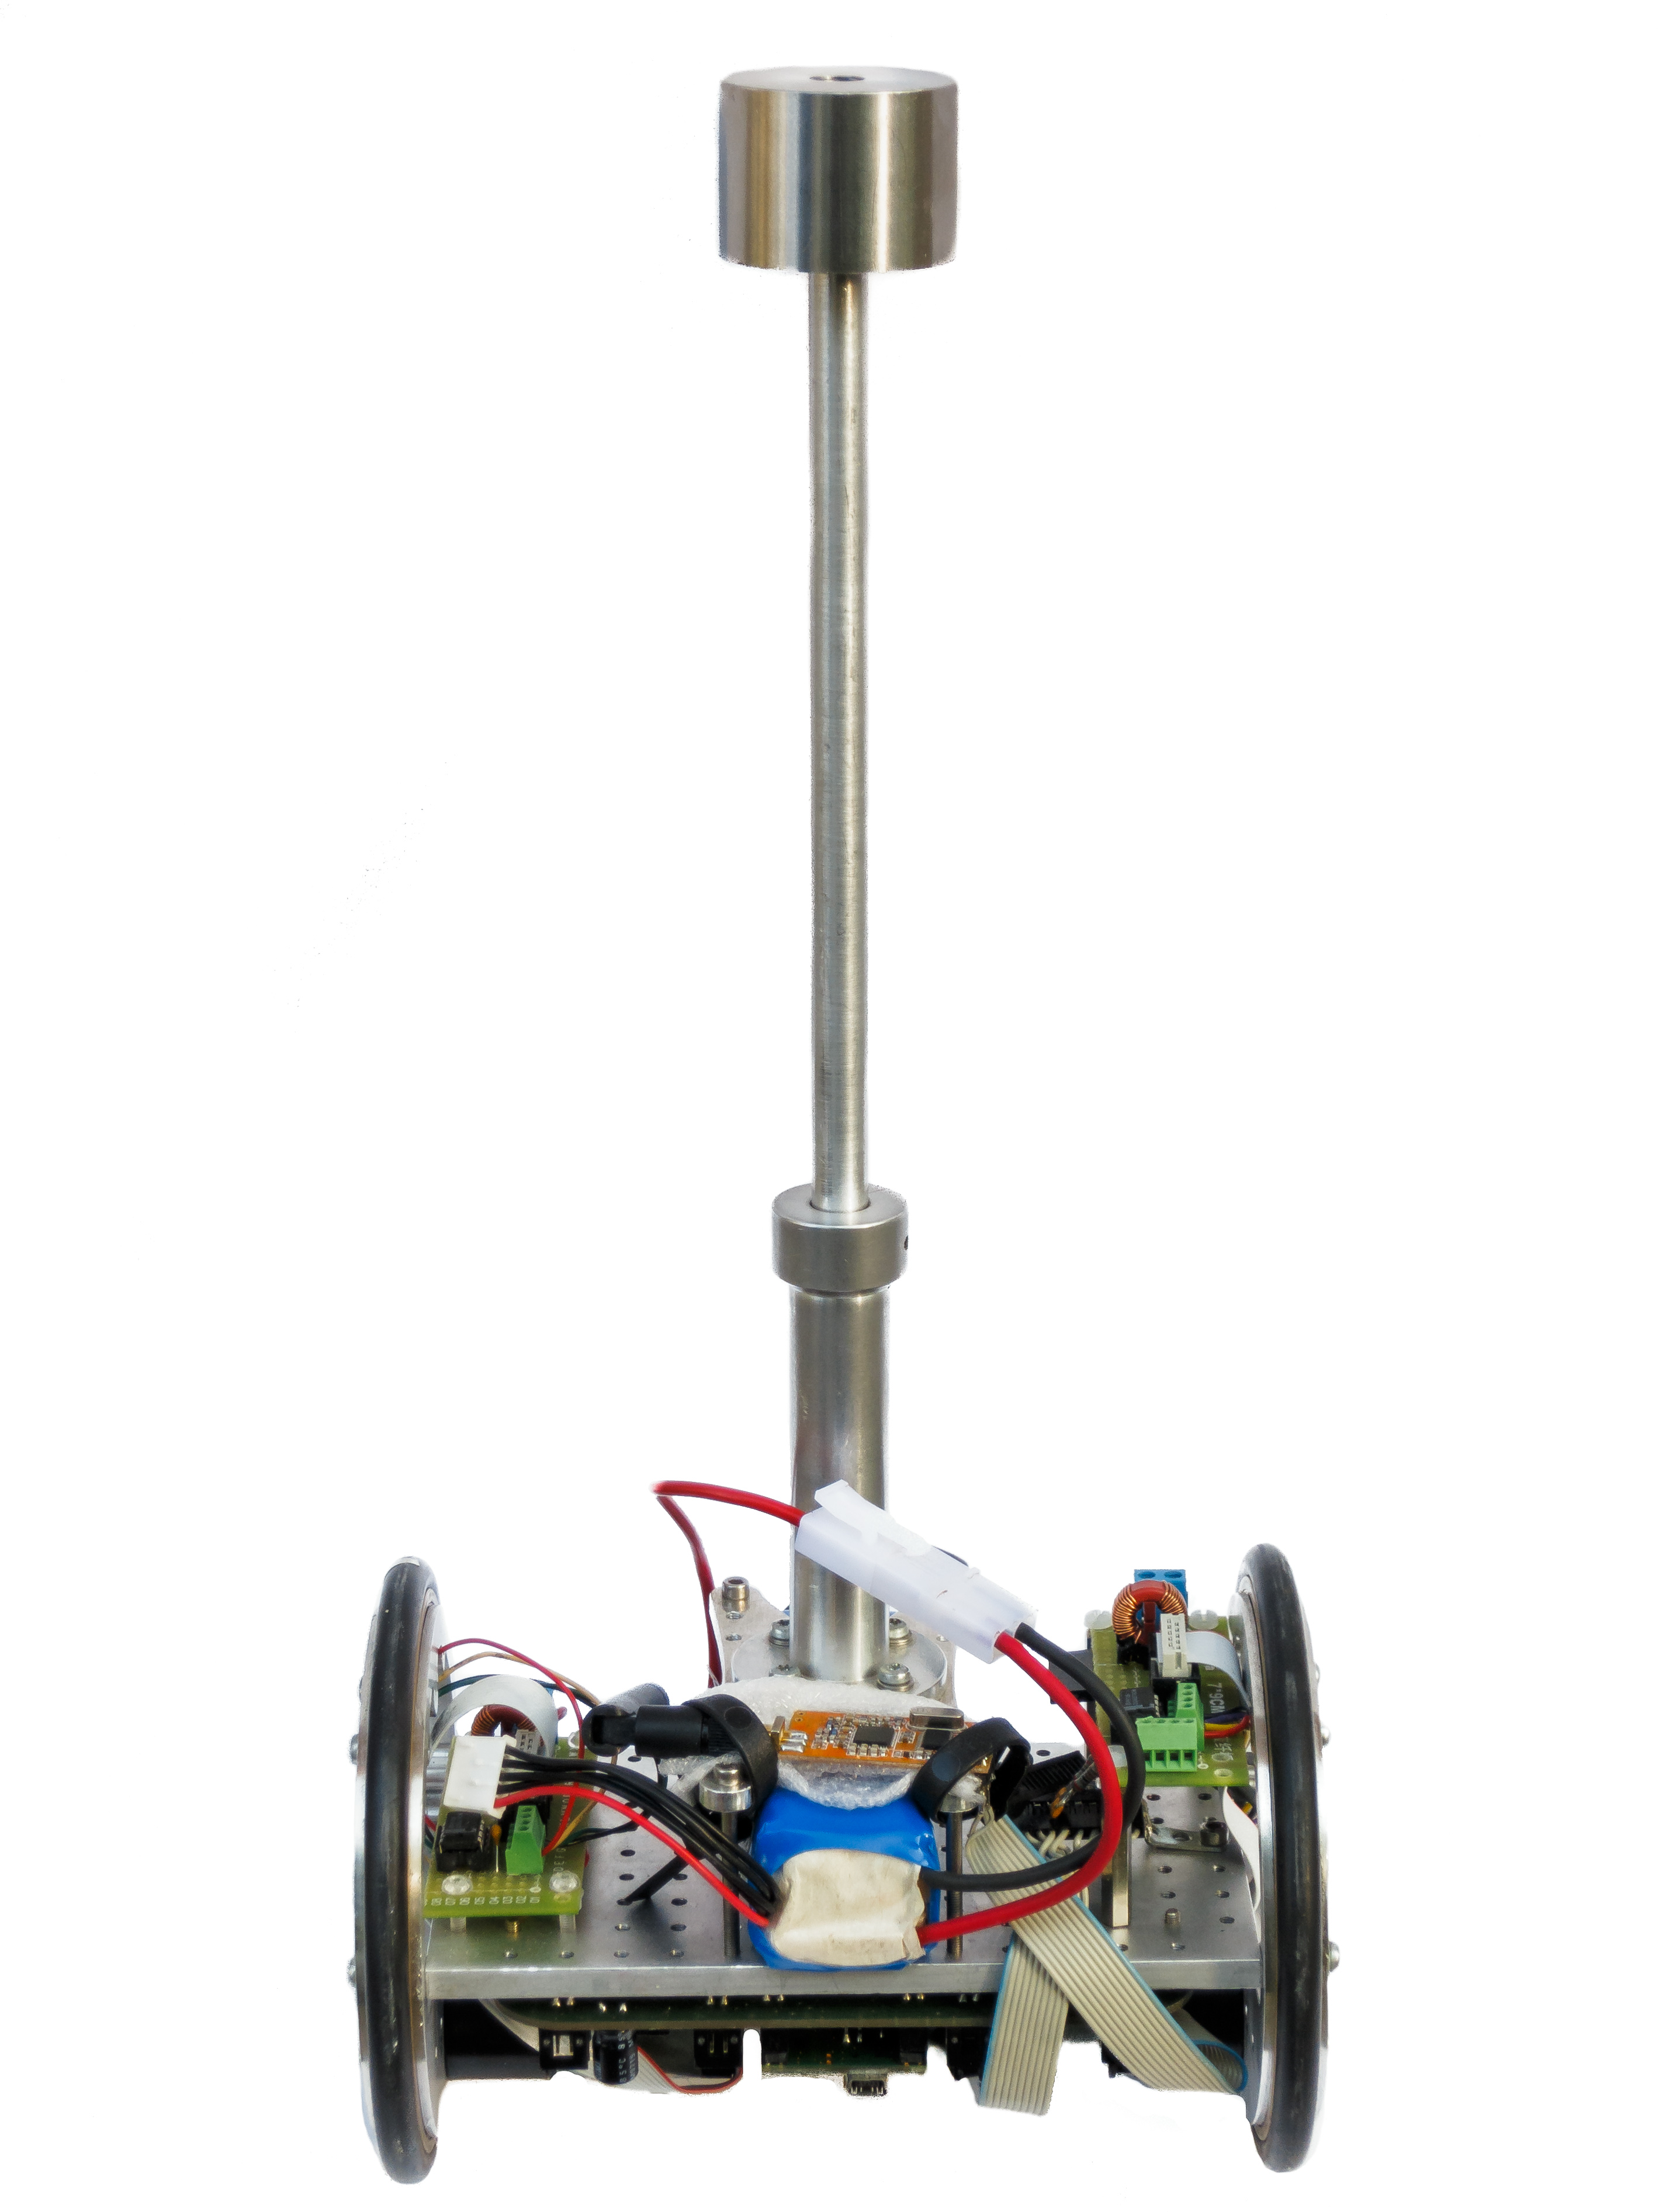
\includegraphics[width=\textwidth]{figures/hardwarePlatform.jpg}
	\caption{The segway to be used in the project (approx. height is 37 cm)}
	\label{minisegway}
	\end{minipage}
\end{figure}
%\todo{why is this interesting to work with}
\vspace{-3mm}
The inverted pendulum has found a new application in recent years, namely in the form of the segway. A segway is a small vehicle that can be used for human transportation where the user stands on a platform placed between two wheels.

%\begin{figure}[H]
%\centering
%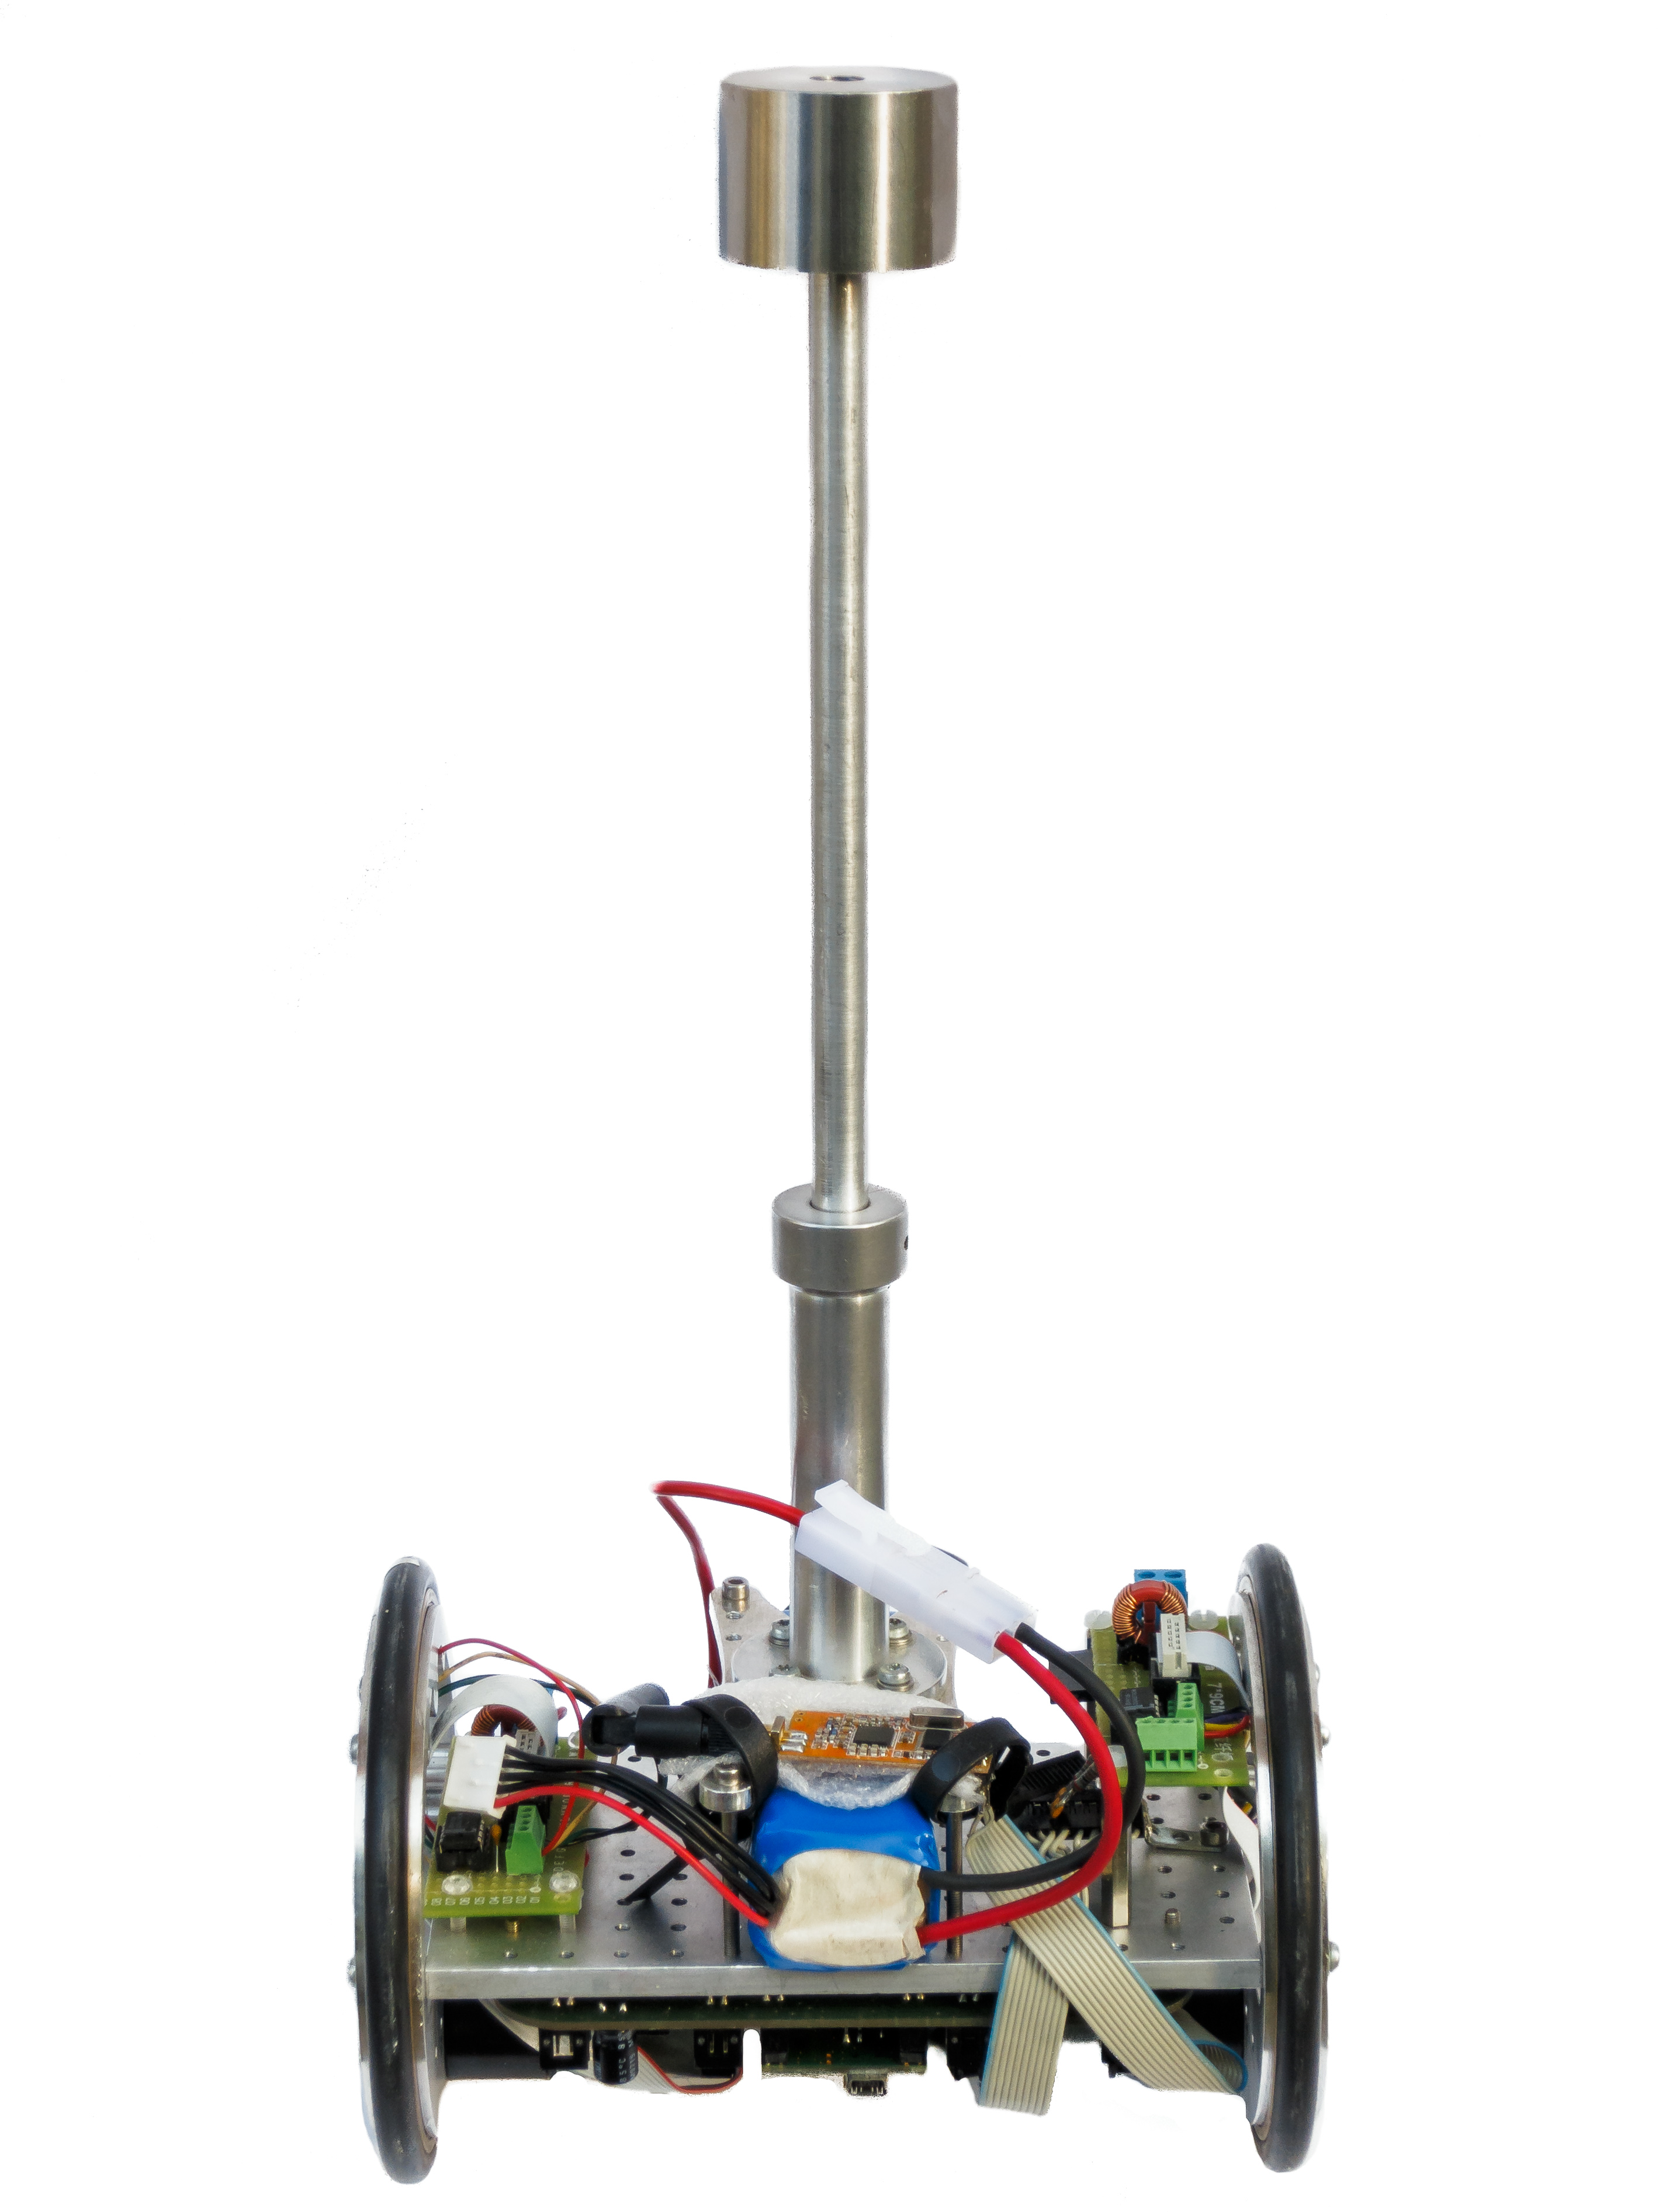
\includegraphics[width=0.4\textwidth]{figures/hardwarePlatform.jpg}
%\caption{The minisegway to be used in the project}
%\label{fig:minisegway}
%\end{figure}

This project concerns the development of a controller for a pre-manufactured segway provided by Aalborg University as can be seen in \autoref{minisegway}. This controller is to stabilize the inverted pendulum in it's upright position, and control the segway's position. The segway is seen as toy to be driven around indoors, and not as a model of a full-size segway. Because of this, all mentions and analyses of a segway throughout the report is in regards to the segway, and not a full-size segway.\\
In the following chapter, a presentation of the general workings of segway is presented.
%In order to control the balancing and driving of the segway, a controller has to be implemented. A good solution is to make the remote control wireless. %Therefore, a wireless remote for the segway will be discussed later on. \todo{a bit rough introduction to remote controller requirement}



%Before the actual modelling and controller design can take place, a presentation of this platform done in the following chapter.


%in particular the modelling and control needed to make the segway self-balancing.
%Ralf's suggestions:

%The inverted pendulum is a classical control problem, in which a pendulum, usually hanging beneath the pivot point, is inverted so that it hangs above.
%
%Whereas a regular pendulum is a stable system with a resting position, the inverted pendulum is inherently unstable. This means that unless some action is taken, the pendulum will fall over by itself. 
%
%The inverted pendulum has found a new application in recent years, namely in the form of the segway. A segway is a means for transportation, where the user stands on a platform placed on two wheels. The segway moves in the direction the user moves, i.e. if the user leans forward, the segway moves forward.
%
%This project concerns the development of a segway, in particular the modelling and control needed to make the segway self-balancing.

\chapter{Segway Presentation}
In the following chapter, an overview of how a segway works is presented. This includes a block description of the system, and a description of the functionalities	 it is to have.
The segway provided by Aalborg University is also described, in regards to the mechanical frame and the provided hardware.

\section{Generalized Segway Description}
A segway can be seen as a typical control system, as shown in \autoref{fig:seg_over}.
Here, the controlled parameters are acquired using various transducers, processed by the system controller and then a control signal is outputted to the actuator(s) through. Apart from the control system, a \gls{RC} is added to the system, which can also be seen in \autoref{fig:seg_over}. The reason for this will be described later on. In the case of the segway, the transducers are sensors, providing information on the movement of the segway, and the actuators are motors, which are driving the wheels. 

\begin{figure}[H]
\centering
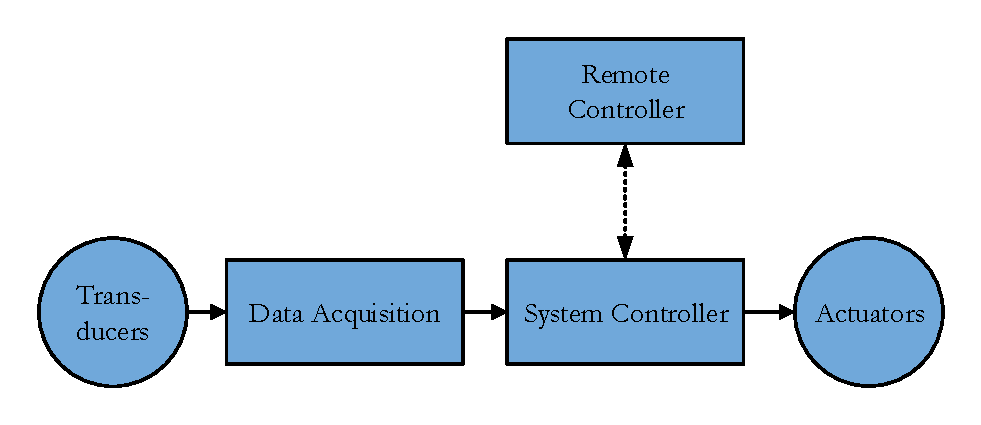
\includegraphics[width=0.7\textwidth]{figures/segwayOverview.pdf}
\caption{Generalized block diagram of a segway control system.}
\label{fig:seg_over}
\end{figure}

It is decided that the segway is to have four main functionalities to function as desired. These functionalities are \textit{balancing, driving, turning and the ability to be remote controlled}. Each of these are described in further detail in the following section.

\subsection{Functionalities of the System Controller}
The controller unit has four main functionalities, namely balancing, driving, turning, and transceiving wireless signals between the \gls{RC} and the system controller. Each of these functionalities are described in further detail in the following section.

One of the required functionalities of any segway is the ability to balance. The system controller must control the motors so the inverted pendulum is balancing vertically. Because the pendulum is unstable by nature, the controller has to make the system stable. This functionality relies on input from the transducers, which is used to calculate an actuator signal to keep the segway balanced.

%The movement and control of the system can be based of the current state of the segway measured by transducers. The transducers can for example tell about the current position, speed, and acceleration of the segway. 

%The data will then be processed in the microcontroller which determines how the segway should react to the current state.

%\subsubsection{Transceiving of wireless commands}
Through a wireless RC the segway is remote controlled. This means that the segway must be capable of receiving commands from the RC and make the segway move accordingly. To achieve this, the segway and RC must share a communication protocol. The wireless RC should also able to receive information regarding the movement of the segway like the speed, angular velocity and angle.

%\subsubsection{Driving and turning}
The driving and turning functionalities are responsible for controlling the segway's forward and backwards velocity as well as the direction of the segway. To ensure the segway does not fall over when driving or turning, the movement will of course have to happen in corporation with the balancing functionality, since balance is still to be kept when driving and turning.

%The velocity of the segway can be controlled by changing which angle the balance functionality tries to uphold. To keep this new angle, the balance functionality must respond to the change in angle, by changing the translatoric velocity. In other words, the rotational moment must be countered by an equal translatoric force.

%Unlike the driving functionality, the turning functionality does not lead to changes in the balance functionality, since turning is rotation around a different axis.

%These functionalities are in the same control unit as they must correlate with the balance functionality, since the output of both the balance, driving and turning functionalities must be merged before it is sent to the motor control unit.

%\chapter{System presentation}
%Aalborg University has provided the project group with a pre-built mini segway. Based on the system design of an segway this chapter will, present and describe the mini segway, with a focus on the mechanical frame and the provided hardware. 
\section{Description of Provided Segway} \label{sec:hardware}
Before the modelling and the design of the controller can begin, the segway provided by the university first has to be described, especially in regards to the electronic hardware used on the segway. This is done in the following section. A photo of the provided segway can be seen in \autoref{hardwarePlatform}. 

\begin{figure}[H]
	\centering
	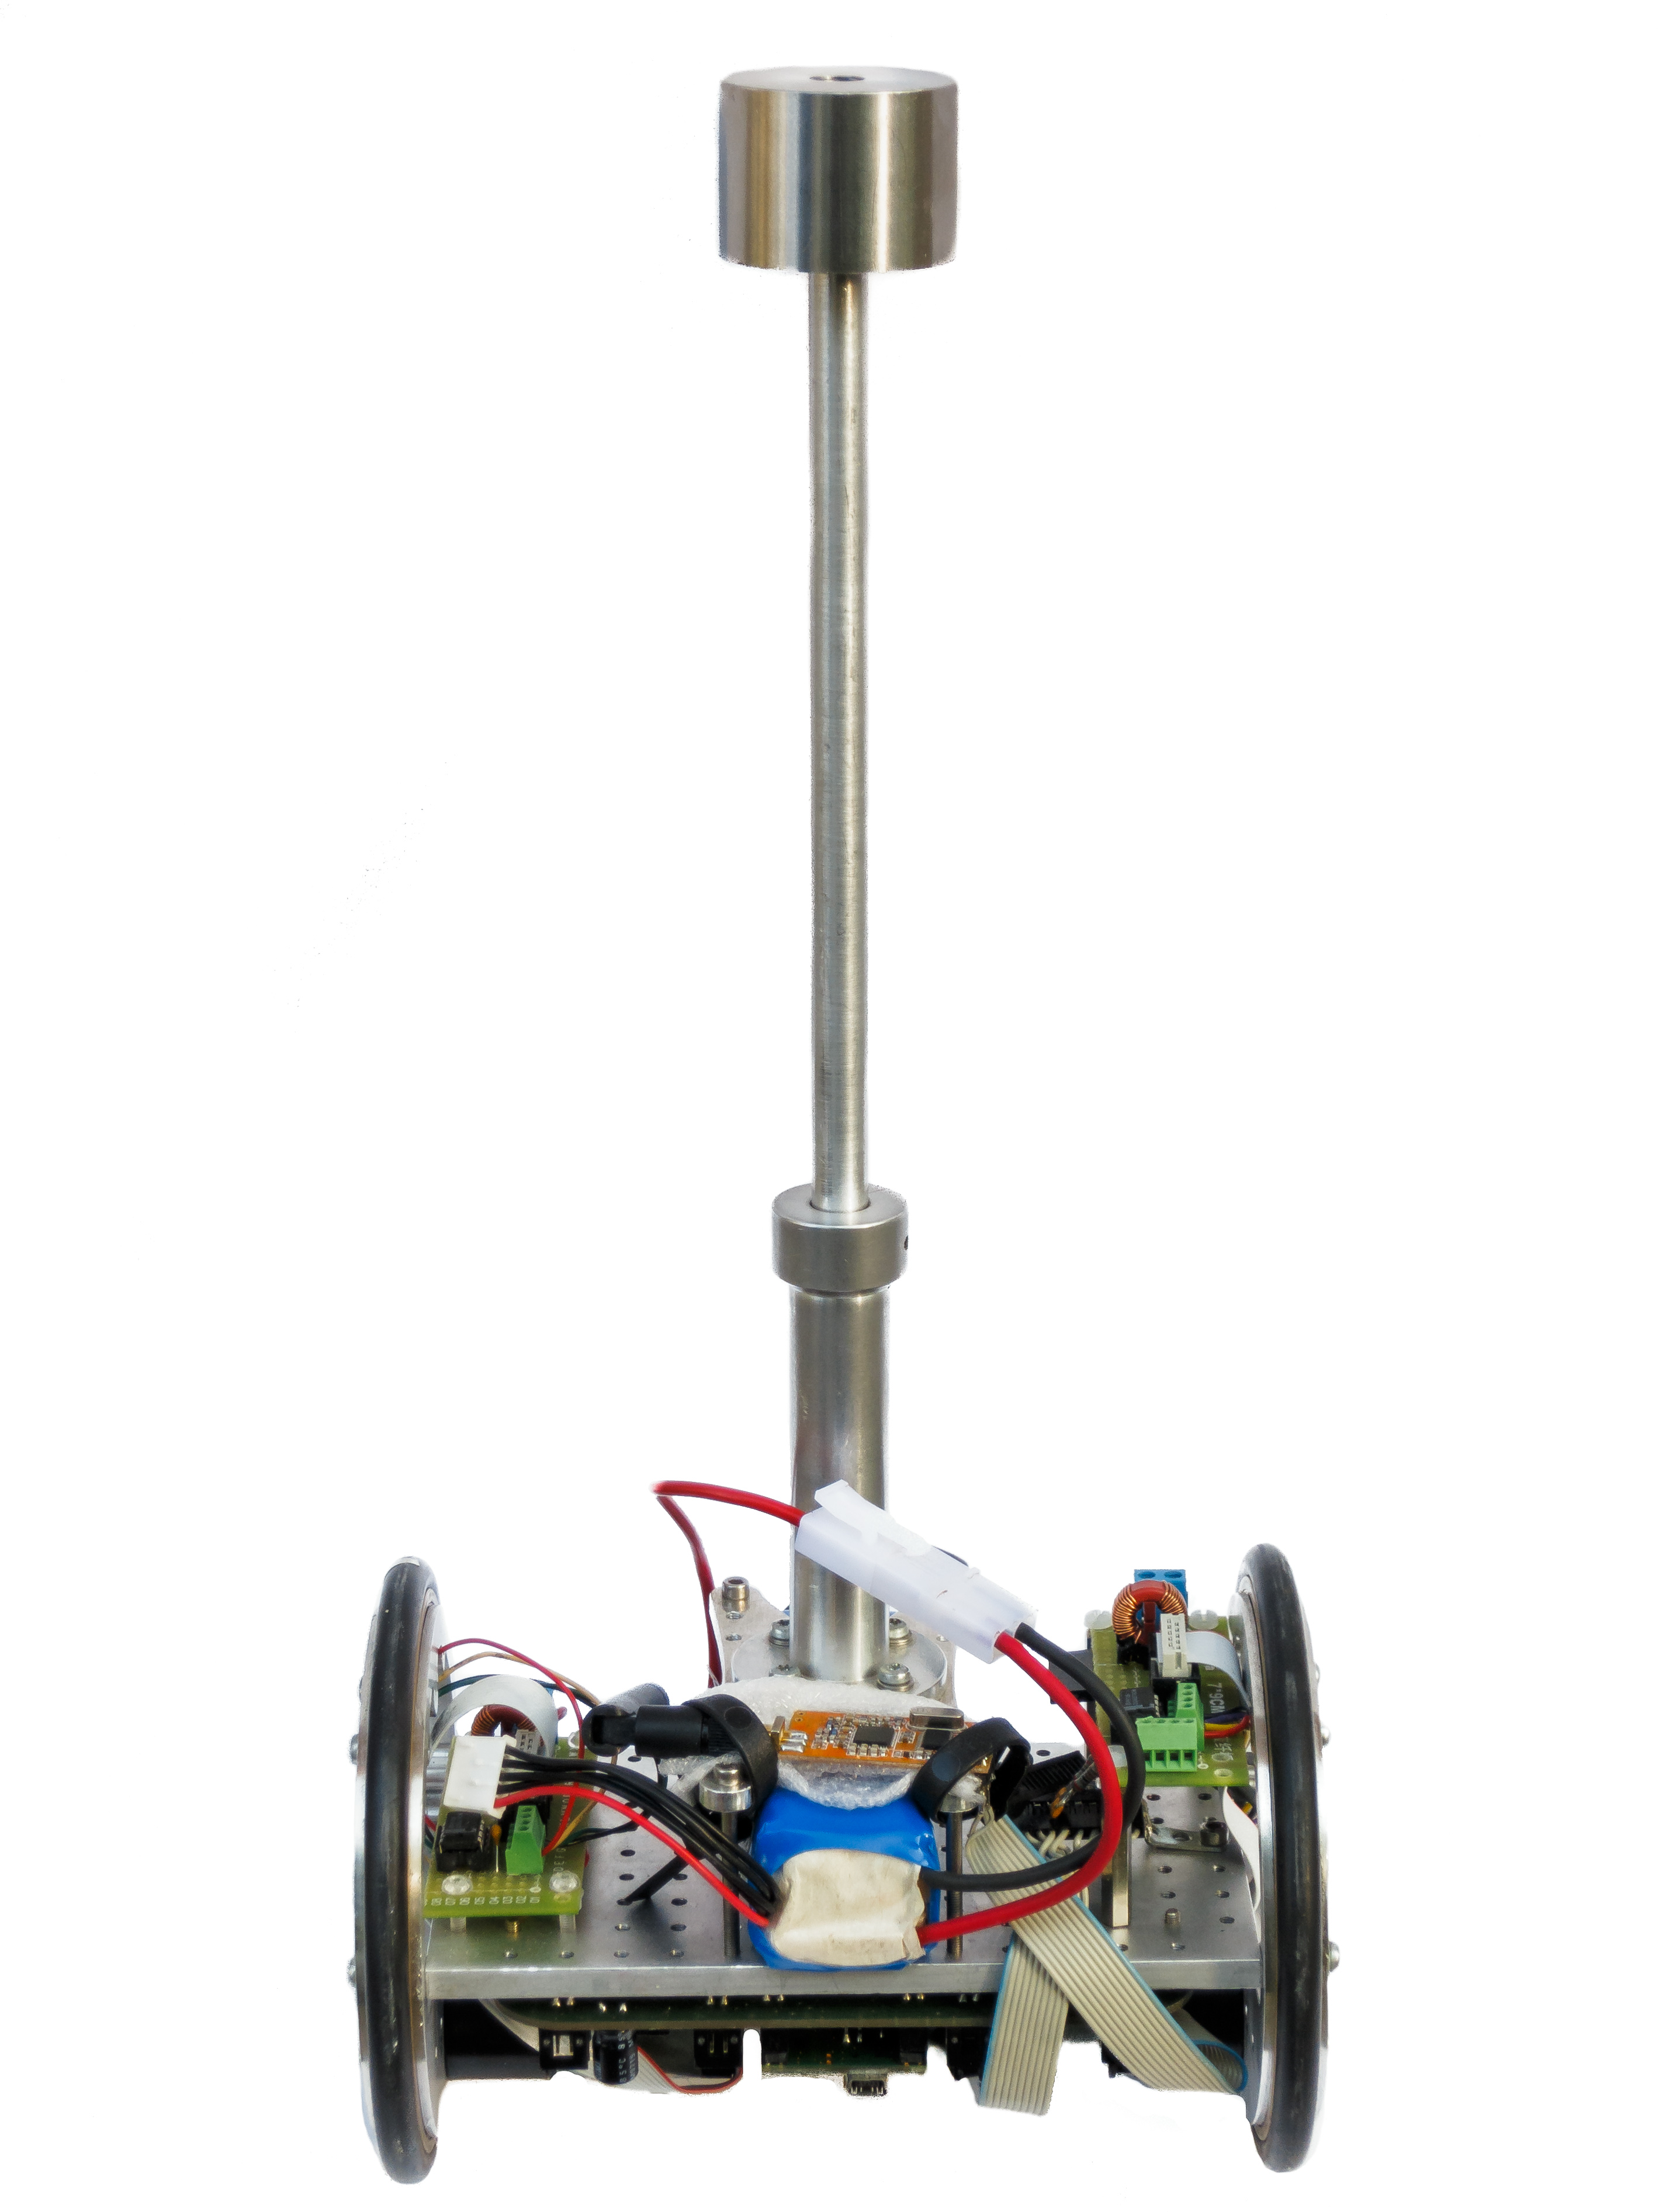
\includegraphics[width=0.4\textwidth]{figures/hardwarePlatform.jpg}
	\caption{The segway to be used in the project.}
	\label{hardwarePlatform}
\end{figure}

The segway consists of several items, these items are divided into 3 main groups, namely \textbf{mechanical}, \textbf{power} and \textbf{electronics}. These groups and the items they include are described in the following.

%\begin{itemize}
%
%\item \textbf{Mechanical}
%\begin{itemize}
%\item Mechanical frame
%\item Wheels
%\item Motors
%\end{itemize}
%
%\item \textbf{Power}
%\begin{itemize}
%\item Batteries
%\item PSUs (Power Supply Units)
%\end{itemize}
%
%\item \textbf{Electronics}
%\begin{itemize}
%\item Wireless transceivers
%\item Microcontroller
%\item Filters
%\item Accelerometer + gyroscope
%\item Motor driver
%\item Encoders
%\end{itemize}

%\end{itemize}
%\todo{remove list, write as text}
%These will be described in further details in the following.

\subsection{Mechanicanics}
\subsubsection{Mechanical Frame}

The provided segway's mechanical frame is made from aluminium. It consists of a baseplate onto which the wheels are mounted, together with a rod with a cylindrical mass on top. All electronics including batteries are mounted on the baseplate.

A blueprint of the segway can be seen in \autoref{segwaySchematic} in \appref{app:segwayParameters}, and measurements of relevant parameters of the frame is listed in \autoref{tab:dimensions}, also in \appref{app:segwayParameters}.


%\begin{wrapfigure}{R}{0.5\textwidth}
%\centering
%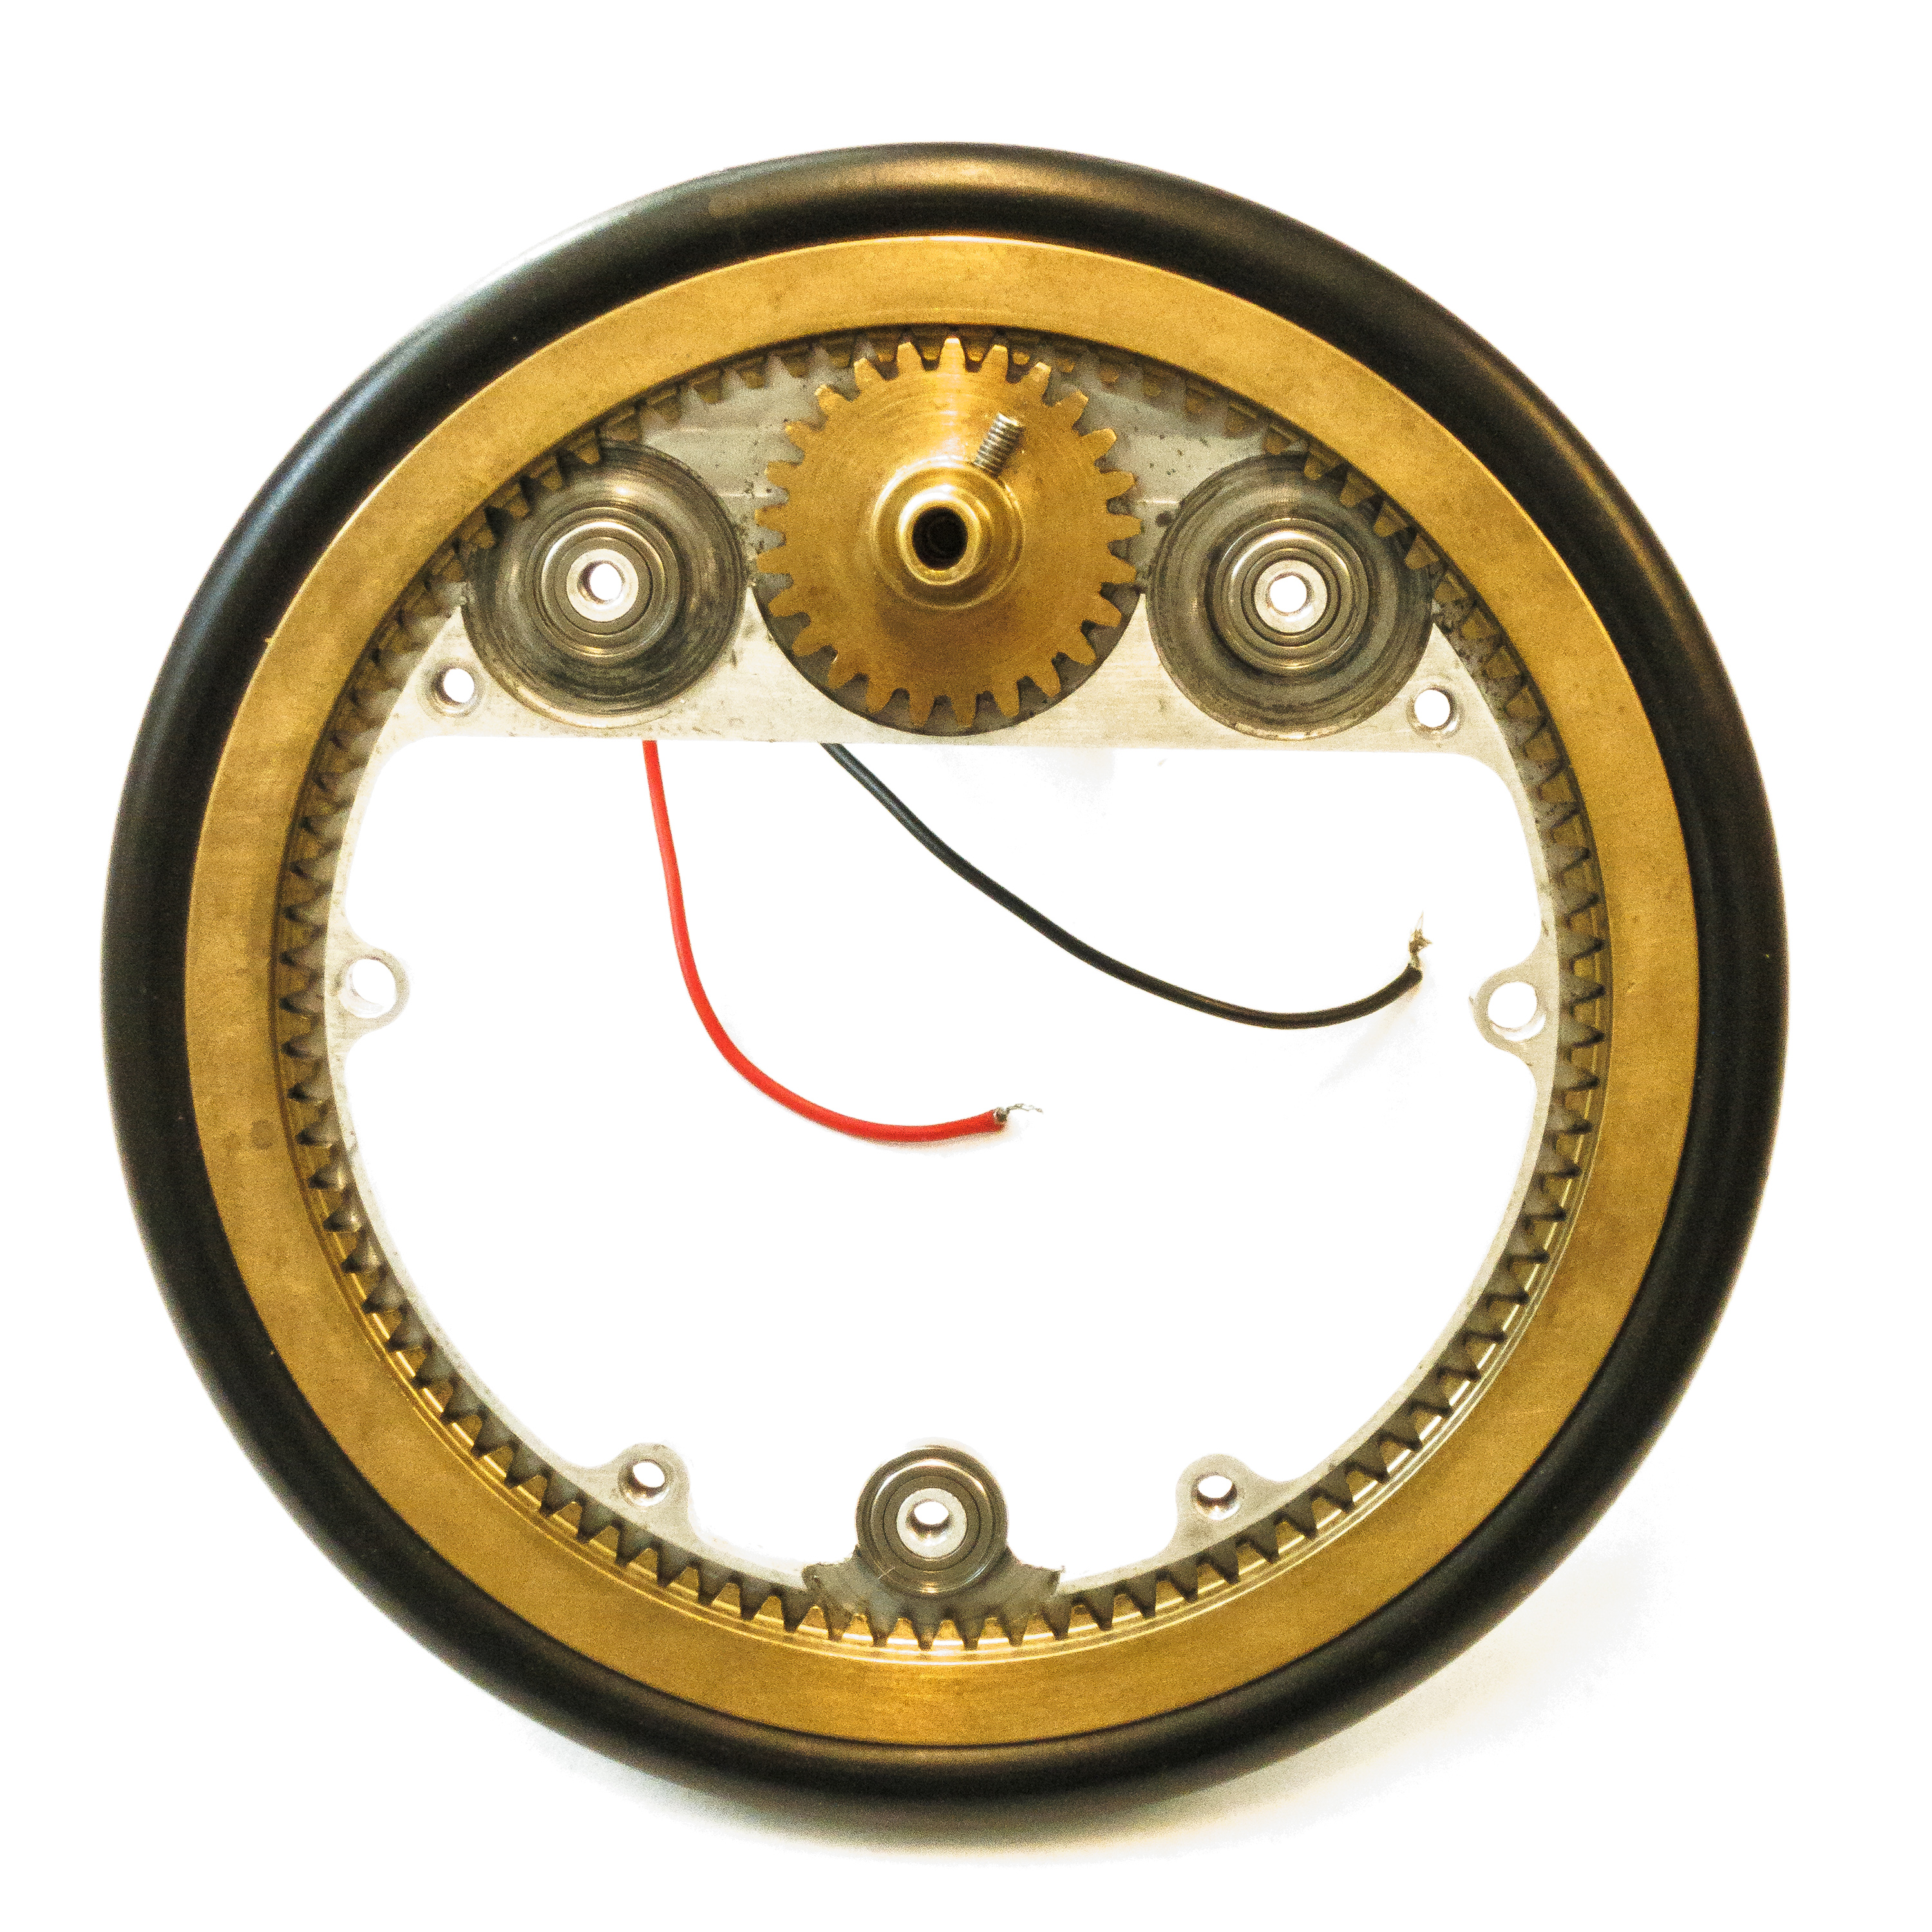
\includegraphics[width=0.4\textwidth]{figures/wheel.jpg}
%\caption{The wheel and motor showing the transmission(motor behind the small gear)}
%\label{fig:wheel}
% \vspace{-4cm}
%\end{wrapfigure}


\subsubsection{Wheels}
\label{subsec:wheels}
The wheels mounted on the segway feature an offset motor, meaning the motor is not mounted at the center. Though, as seen from the blueprint in \autoref{segwaySchematic} in \appref{app:segwayParameters}, the axis of the wheel is still in the center of the base. The wheel system is built as follows: The motor rotates a gear fitted onto the motor from the factory. The shaft from this gear is located on the inner side of the wheel, and mounted to a cogwheel. The inner side of the wheel itself has some small cogs making it the other part of the transmission system.
For a better rotation and less friction, the wheel has three ball bearing guides. This can be seen in \autoref{fig:wheel}.
The cogwheel mounted on the motor wheel has 25 cogs and the inside of the wheel has 90 cogs.

\begin{figure}[H]
\centering
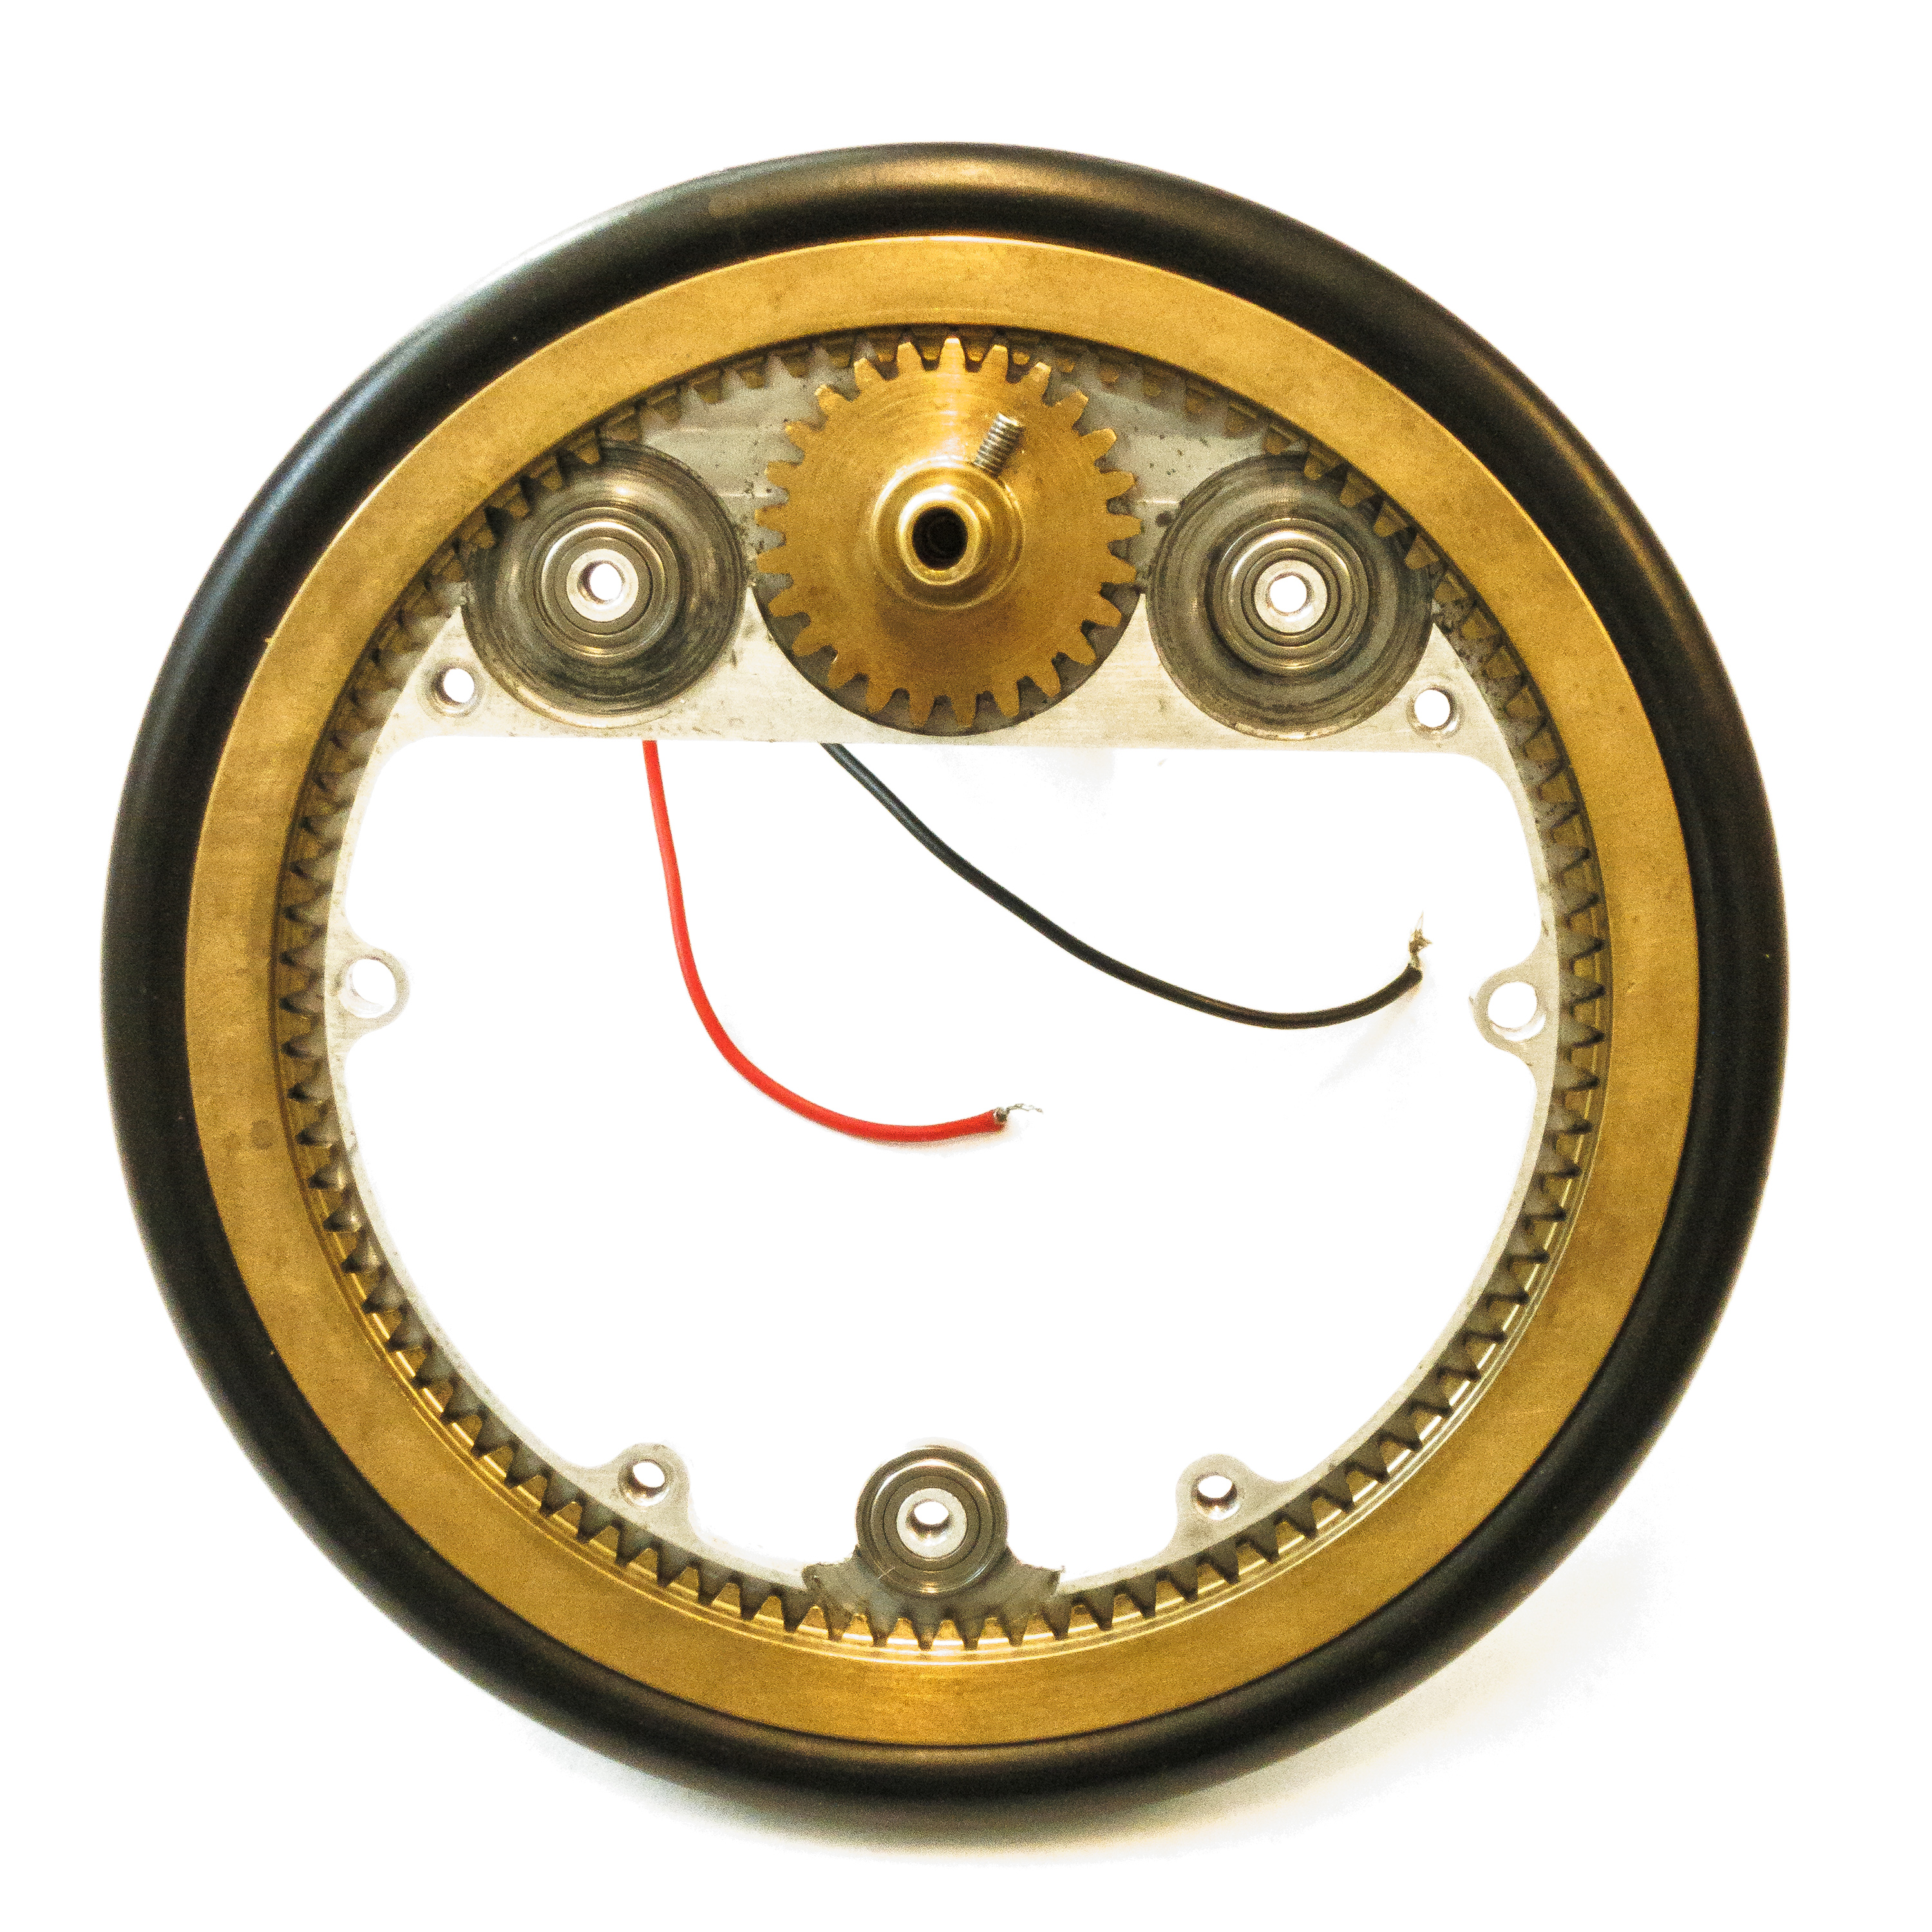
\includegraphics[width=0.4\textwidth]{figures/wheel.jpg}
\caption{The wheel and motor showing the transmission. The motor is behind the small gear.}
\label{fig:wheel}
\end{figure}

\subsubsection{Motors}
\label{subsec:motors}
The segway uses two Maxon A-Max 110160 permanent DC-motors to rotate the wheels. Parameters of the motors that might be taken into account are the rotational speed and the torque. The specification of the motors are \citep{maxon}
\begin{itemize}
\item Nominal torque at {6 V} is 5.91 mNm.
\item Nominal speed at {6 V} is 6240 RPM.
\end{itemize}

%A permanent DC motor is working by rotating an armature within a magnetic field. This produces a mechanical force, when a current carrying conductor is placed in the magnetic field, as this is exerting an equal and opposite force due to Newton's third law. 

%The rotational speed is given in RPM (Revolutions Per Minute) and the torque is given in mNm (milli Newton meter).

The motors are brushed, meaning the stator corresponds to the magnets and the rotor is composed of the coils, receiving power through brushes.
Brushed motors have important advantages: They have a low cost of construction, require only simple and inexpensive control and they operate in extreme environments due to lack of electronics. However, those motors also have drawbacks: They require periodic maintenance, their characteristics are moderately flat and at high speeds, brush friction increases, thus reducing useful torque. Also, the brush arcing will generate noise causing electrical magnetic interference (EMI) \citep{BvsBL} \citep{BvsBLv2}.

\begin{figure}[H]
	\centering
	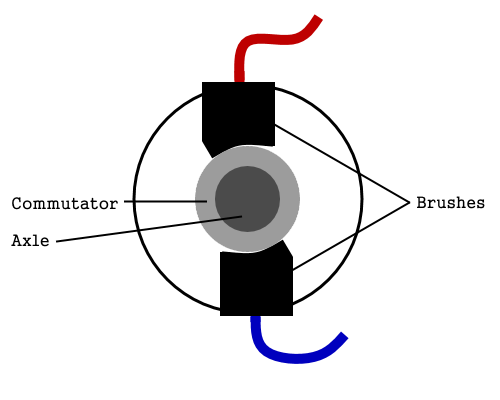
\includegraphics[width=0.5\textwidth]{figures/brushed_2.png}
	\caption{Sectional view of a brushed motors.}
	\label{DCBrushed}
\end{figure}

As a part of the motors, a gear (Maxon 110356) has been fitted on the motor. This gear was fitted from the factory, and the inner workings of it are therefore not known. From the datasheet, the gear ratio between the motor and shaft is known \citep{gear}: 
$$N_{ms} = \frac{1}{19} \approx 0.053$$

\subsection{Power}
\subsubsection{Batteries}
The segway comes equipped with a battery which is the source of power of the system. The battery is a rechargeable 4S LiPo. LiPo batteries, or Lithium-ion Polymer batteries, consists of cells in series, \textit{x}S meaning \textbf{\textit{x}} cells in \textbf{S}eries. A LiPo cell has a nominal voltage of 3.7V. The battery used on the device has a nominal voltage of 14.8 V (3.7 Volts times 4 cells).
LiPo batteries, compared to other types such as Nickel–metal hydride (NiMH), one of the most common battery types, are lighter and more compact. However, they are more expensive than "regular" batteries and require a specific charger to bring every cell of the pack to the same state of charge \citep{Cells}.

The Segway also has two Power Supply Units (PSU's). These are electronic components, whose role it is to regulate the unstable input voltage from the batteries, to a stable voltage to be used by the electronics.
One has an output of 5V and the other has an output of 3.3V. 

\pagebreak 
\subsection{Electronics}
\subsubsection{Wireless Transceivers}
To facilitate the wireless communication between the segway and a remote controller, a pair of APC220 radio communication modules is supplied.
The modules have the following features \citep{wifimodule}:
\begin{itemize}
\item Transmission distance of up to 1000 m (2400 baud)
\item UART/TTL interface with 256 bytes data buffer
\item -112 dBm sensitivity at 9600 baud
\item 20 mW output power
\item Adjustable frequency from 418 MHz to 455 MHz
\end{itemize}

Since the modules have a UART interface, they can be interfaced through a UART interface on a microcontroller, which makes the radio modules simple and easy to use.

\subsubsection{Microcontroller}

A microcontroller board is supplied with the segway. The \gls{PCB} on which all the electrical components are mounted, is designed to fit the supplied \gls{MCU}, and thus a new MCU is not chosen, since it might require a redesign of the PCB.

The microcontroller board supplied is a \emph{CrumbX128A3} made by Chip45 \citep{CrumbX128A3}. The CrumbX128A3 features an ATxmega128A3U microcontroller, a 3.3V low dropout (LDO) voltage regulator, a USB UART converter, an RS485 transceiver and a micro-sd-card header/slot.
	
The ATxmega128A3U has the following specifications \citep{xmega}:

\begin{itemize}
\item 32 MHz clock speed
\item $1.6-3.6$ V power supply
\item 128 Kb flash
\item 8 KB SRAM
\item 7 UARTs
\item 7 16-bit counters
\item 4-channel DMA controller
\end{itemize}
\subsubsection{Accelerometer and Gyroscope}
To measure the angle the segway is tilted as well as its relative position, an accelerometer and gyroscope is used. Here, the InvenSense MPU-6050\citep{gyro} is used, a 6-axis gyroscope and accelerometer. The chip is implemented on a GY-521 breakout board. It features an \iic bus, from which the raw sensor values can be read. 
The gyroscope can be configured to having a full-scale range of either $\pm 250, \pm 500, \pm 1000$ or $\pm 2000 \degree /\text{sec}$. The accelerometer can be programmed to have a full-scale range of $\pm 2g, \pm 4g, \pm 8g$ or $\pm 16g$ \citep{gyro}.

\subsubsection{Motor Driver}
To control the motors, a motor driver is used, in form of an H-bridge. The H-bridge allows a small controller-voltage to control a (often relatively large) current. This is practical, since the current needed to drive most motors is bigger than what can be drawn from the pins of a microcontroller. 
Here, two Freescale MC33926 5A H-bridges \citep{hbridge} are supplied - one for each motor. The H-bridge makes it possible for a motor to be run both forward and backwards, based on the input signals to the chip. It also features a feedback-pin, also known as a current sense, that can be used to measure the current drawn by the motor. The H-bridge is controlled by an input PWM signal and two direction pins. By setting these pins, the motor can be either locked, free-running or moving forwards or backwards.

\subsubsection{Encoders}\label{subsec:preEncoder}
In order to keep the inverted pendulum in balance, the segway needs a way to quantify the amount of rotation on the wheels and, by extension, on the motors, hence the encoders. The ones currently used by the system are relative (or incremental) encoders placed directly on the motors.
An incremental encoder delivers a certain number of pulses per revolution. This number of pulses measures the angular movement.
Usually, relative encoders consist of a disc divided in transparent and opaque segments. Most of those discs are equipped with two rows of segments plus a top segment. Both segment tracks are slightly out of phase to indicate the direction of rotation and the additional top segment allows the count of revolutions.
An incremental encoder's resolution corresponds to the maximum number of pulses sent per revolution and is symbolised by the unit "points per rotation" \citep{IncEnc}.
\vspace{-1 cm}
\begin{figure}[H]
	\centering
	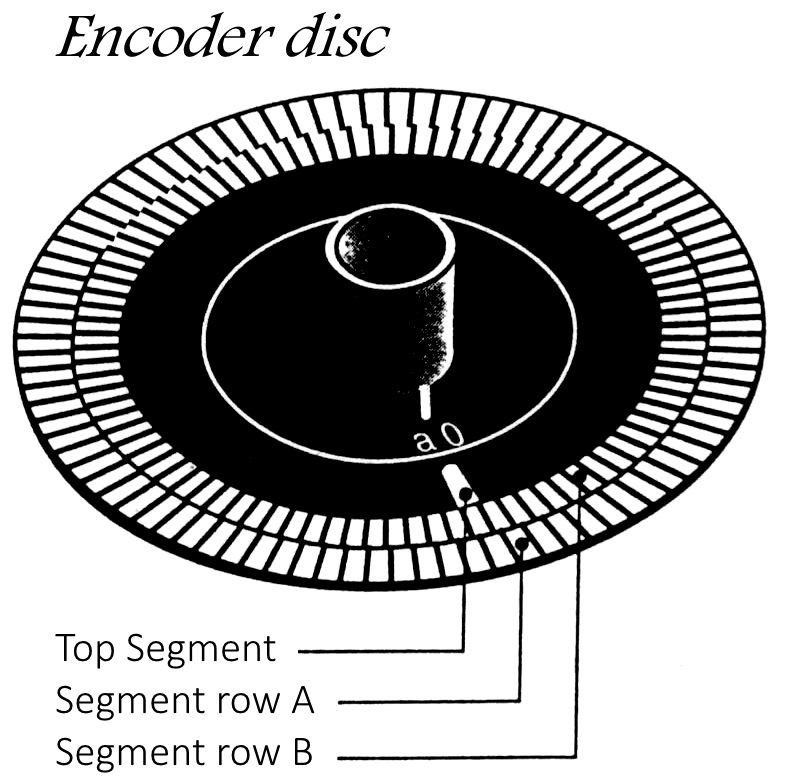
\includegraphics[width=0.36\textwidth]{figures/Encoder.jpg}
	\caption{Detailed scheme of an incremental encoder \citep{IncEnc}.}
	\label{fig:incremental_encoders}
\end{figure}

%Placed between the motor encoders and the microcontroller, are some filters. The filter type used is not known, nor is the filter specifications. Since its inputs and outputs are unknown, it is considered a black box.
%Because of this, it is decided to remove these filters and design new filters, so the exact transfer function of them is known.

\newpage
\subsection{Detailed Segway Overview}
The general block diagram of the segway control system in \autoref{fig:seg_over} can be extended based on the provided hardware described above. The detailed diagram can be seen in \autoref{fig:ext_seg_over}.

\begin{figure}[H]
\centering
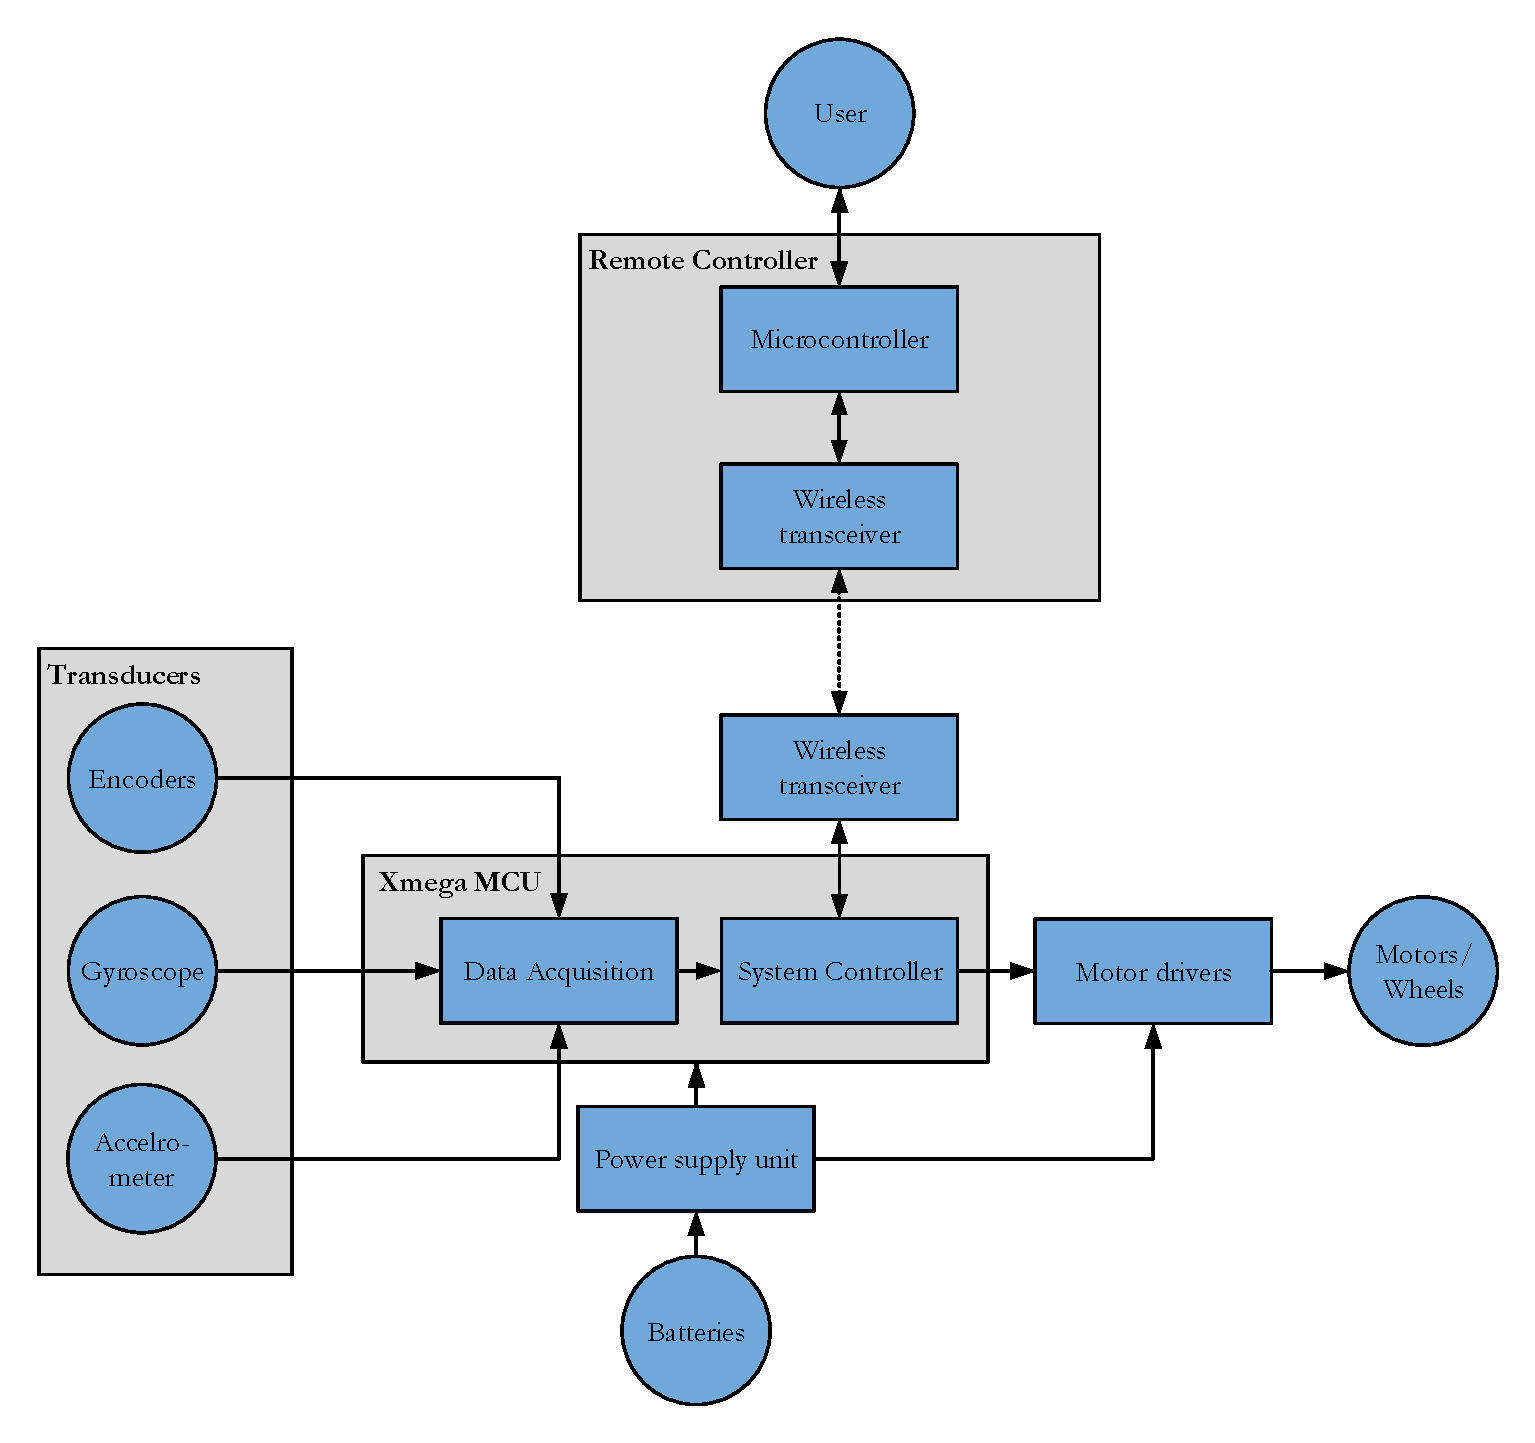
\includegraphics[width = 0.95\textwidth]{figures/extendedOverview.pdf}
\caption{Detailed block diagram of the segway system.}
\label{fig:ext_seg_over}
\end{figure}

In the detailed diagram, the different transducers have been added, and the functionalities the MCU is to facilitate have been grouped. Also, the actuator has been specified, in the form of motors.
The workings of the remote controller are also described in further details, namely that it is to receive user input to a MCU and then transmit it wirelessly. It can also display data from the segway to the user. Also added to \autoref{fig:ext_seg_over} are the batteries and PSUs. 


\section{System Overview}

Before the design of segway can begin, it has to be determined which subsystems are to be designed. In \autoref{fig:ext_seg_over}, the detailed block diagram of the system was presented. As most of the hardware for the segway is already provided, the project will primary focus on designing the controllers in the system. This limitation can be seen in \autoref{fig:system_overview_block}. Here, the blue blocks are subsystem that are to be designed, while the grey blocks are not designed.


\begin{figure}[H]
	\centering
	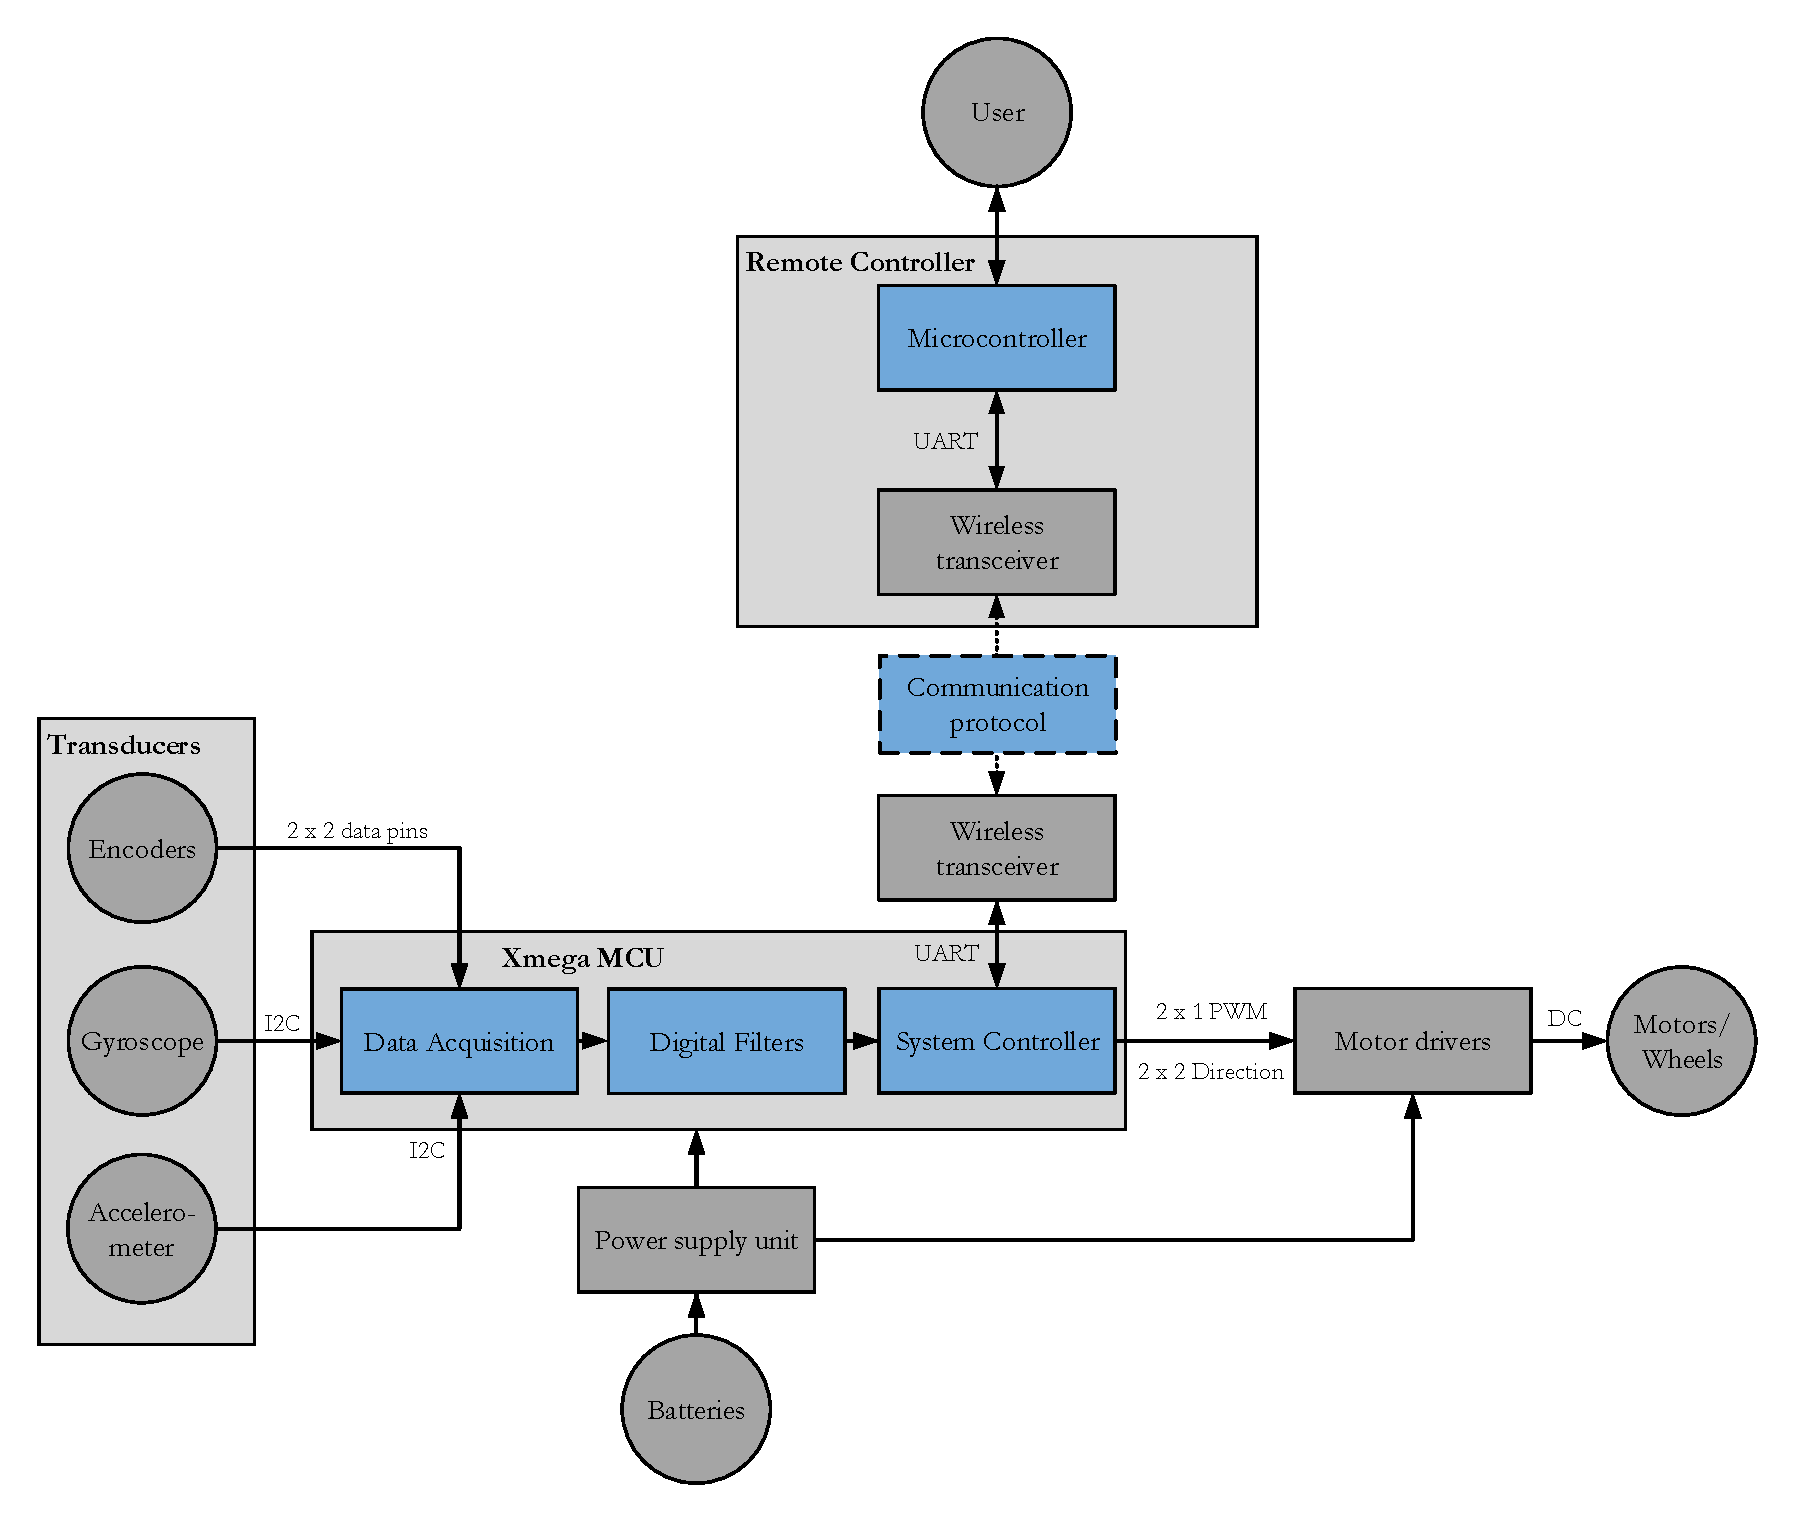
\includegraphics[width=0.95\textwidth]{design/figures/extendedOverviewGrayedWithInterfaces.pdf}
	\caption{Overview of the system. The blue blocks are blocks the design primary deals with.}
	\label{fig:system_overview_block}
\end{figure}
Note that a communication protocol has been inserted between the wireless transceivers. This is done because some "rules" has to be introduced in the communication between the remote controller and the MCU on the segway to ensure a proper data transfer without misunderstandings.

Also, a filter is inserted between the encoders and the MCU. To avoid breaking electrical interfaces and changing the electrical configuration of the segway, the filter is implemented as a digital filter, instead of an analog.

To ensure that subsystems can be designed parallel, the interfaces between subsystems have to be clarified. Data types transmitted between subsystems are shown in \autoref{fig:system_overview_block}. From left, the gyroscope and accelerometer transmits measured values through an $I^{2}C$ communication protocol, and the encoders data through two data pins. For external communication to the remote controller, data is transferred through a UART interface which is supported by both the wireless transceiver and the microcontroller. To control the motor drivers, a PWM signal is used for each motor, together with two direction pins.

\subsection{Control Loop Overview}\label{controlLoopOverview}
The system that controls the balancing of the segway can be described as a closed loop system, as shown in \autoref{fig:segOverview}. The segway is balanced through the use of three subsystems, namely the controller (D), the plant (G) and the sensors (H). It is assumed that the sensors are ideal, meaning that their frequency response is equal to unity i.e. $H(s) = 1$, as this block won't include any amplification or filtering, but solely measure. This is done since it is decided not to determine the sensor's transfer function, and that it will make the calculations easier by assuming that the measued output data is identical to the actual output. The input, R, is the desired angle of the segway, which for the balancing functionality, will be zero, i.e. the steady state upright position. The output $Y$ is the actual angle of the segway, denoted as $\theta_p$.

\begin{figure}[H]
\centering
\input{figures/modelBlockOverview.ralf}
\caption{A feedback loop of the system that controls the balance of the segway.}
\label{fig:segOverview}
\end{figure}

The plant is based on a model of the system that describes the movement of the segway, where the output is $Y = \theta_p$. This model is found in \autoref{ch:modelling}. %The input to the plant model is determined in \autoref{ch:modelling}, where the model is derived from an analysis of the segway. %The plant is used to directly change the output of the closed loop feedback system.

The controller block, D, generates the input to the plant, based on the difference between the desired angle, R, also known as the reference, and the actual angle measured by the sensor system, H. The output of the controller, U, is generated so that the error between output of the plant, Y, and the desired angle is minimized. The design of the controller unit is performed in \autoref{ch:Controller}.

%In the following chapter, the plant model is derived, as this lies the foundation for the controller design.

Now that the segway platform has been described, it is possible to set up the requirements for the system, which is done in the following chapter.



%The interface requirements is needed in order to determine the data type of the inputs and outputs of each subsystem.


%\section{Interface requirements} \todo{The section is still a sketch}
%\todo{reduce section}
%To ensure subsystems can be designed individually it is necessary to define the interface requirements. The interface requirements is needed in order to determine the data type of the inputs and outputs of each subsystem. 
%
%\subsection{Filter}
%
%The input of the filter is an analog signal from the encoders. The signal contains data about the rotation and direction of the motors. Since the inputs from the encoders are analog the best solution, are to make the filter analog as well. \todo{Is the encoder output analog or digital?}
%
%\subsection{Data Acquisition}
%
%As seen on \autoref{fig:system_overview_block} the data acquisition block receives input from the encoders, gyroscope, and accelerometer. Since the microcontroller only operates with digital signals any analog signal from the transducers has to be sampled into digital signal. 
%
%Another task is to convert measured data into understandable data types. This makes it easier to apply the measured data into control algorithm in the system controller.
%
%\subsection{System controller}
%
%Both data acquisition and the wireless transceiver transfers data to the system controller. The input from the data acquisition block is digital data from the transducers. Input from the wireless transceiver is digital as well but the communication protocol has to be the same as on both controllers.
%
%\subsection{Motor controller}
%
%The input of the motor controller is a digital signal from the system controller. The input could be data telling that the segway should move forward. Since the output of the motor controller is connected to the motor driver, it is necessary to insure that data from the motor controller is the same type of the motor driver.
%
%\subsection{Microcontroller for remote controller}
%
%
%
%\subsection{Communication protocol}
%
%
%
%\subsection{User input}
%
%
%
%
%\begin{enumerate}
%\item Modelling
%\item Designing subsystems
%\item System integration
%\item System implementation
%\end{enumerate}





\chapter{Requirements}
This chapter has the purpose of presenting considerations concerning setting up requirements for the the segway. Firstly, the considerations will be made upon a list of requirements set from the preanalysis as well as common sense, for those requirements which has to be set by choice rather than theory. These considerations will result in a list of specific requirements, from which the modelling and controller design of the segway will be designed upon. \\
The requirement considerations follows in the next section.
\section{Requirements Considerations}
The most important functionality of a segway is for it to keep its balance. For this to be achieved, the segway must be able to obtain a stable position after being given an impulse, such as a push. \\
It is preferable to set requirements for the system's step response, as this is a typical measure for a system's dynamic behaviour that is rather easy to measure and set requirements for. In the following, the system's step response's parameters will be described. Afterwards the relation of the system's stability and the phase margin and gain margin will be presented. 

\subsection{Functional Requirements}
For the system, there are some requirements for the overall functionalities of the system. These requirements are derived from intuition, based on what a segway should be able to do.
This includes that the segway has to stabilize itself and balance in an upright position, as well as being able to drive and turn, without falling over. Also, the segway should be able to withstand a light push, without falling over. A "light push" is not defined further, but the push needs to be so big that it makes the segway move in order to stabilize. 
It is also decided that it should also be possible to remote control the segway wirelessly, by means of making the segway drive and turn. The user should also be able to wirelessly receive information from the segway, such as the pendulum angle, $\theta_p$. 

\subsection{Time Domain Requirements}
The step response displays the time behaviour of the system when given an impulse. \autoref{fig:GIR} shows an example of a step response of a dynamic system.

\begin{figure}[H]
\centering
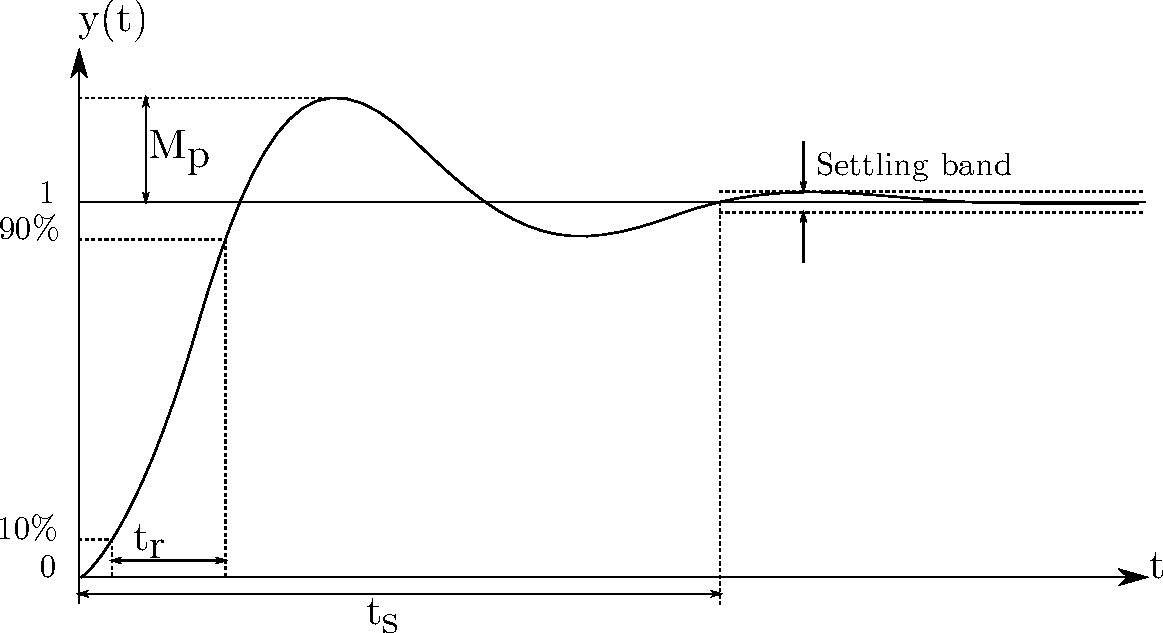
\includegraphics[width = 0.8\textwidth]{figures/steprequ.pdf}
\caption{General step response in time domain. } 
\label{fig:GIR}
\end{figure}
In \autoref{fig:GIR}, the variable $t_r$ is the rise time, defined as the time it takes for the step response to go from 10\% to 90\% of the step. The settling time, $t_s$, describes the time it takes for the system to settle within a certain margin of the final value, typically 1\%, 2\% or 5\%. The steady state error is the difference between the desired steady state value, and the actual steady state value. 
%The variable $t_p$, is the time it takes for the system to reach its maximum value, also called the peak time.
The ratio between the step response's ideal level and the maximum level which the system reaches is the overshoot, $M_p$.\\
To make sure the control system is stable, the system should not have any poles in the right-half-plane of the s-plane \citep[p. 146]{sou:Feedback}, or any poles outside the unit circle, if considering the z-plane \citep[p. 619]{sou:Feedback}.
\\\\
It is desirable not to have a steady-state error, as the balancing of the segway shall be as accurate as possible, to ensure that the angle the segway is to maintain is also met, as an steady-state error in the inverted pendulum angle will cause the segway to move forward or backwards.
It is likewise desirable to have a fast rise time, as it would decrease the risk of the segway of falling over if the controller regulates the segway to an upright balanced position quickly. However, this will result in an overshoot, as the system's quick response to the impulse, for example a push, will make the system overcompensate to minimize the error quickly. This will increase the risk of the segway of falling over, if the overshoot is so high that the segway falls to the other side. The overshoot can also cause oscillations, if the controller constantly tries to obtain the desired angle, but has an overshoot so high, that the overshoot angle also has to be corrected by the controller. Disturbances to the controller making the system unstable, such as the gravity, can affect the way the segway moves forward at a steady velocity. It is important to reduce both disturbances and noise affecting the sensor values, to obtain a control system with high precision.\\
The segway's balance controller shall thus, as with any control system, be a compromise of an agile behaviour, where the settling time is not too long and where overshoot is limited.

The step response is a useful means of evaluating the dynamics of a system, i.e. the rise and settling time, the overshoot and the steady state error. The step is applied to the closed loop, as the step response then includes the effect of the feedback.

The general transfer function for the basic closed loop feedback system is shown in \autoref{eq:GCL} and the corresponding block diagram is shown in \autoref{fig:GCL}. 

\begin{equation}
T(s) = \frac{Y(s)}{R(s)} = \frac{\text{Direct term}}{1 + \text{Open loop}}
\label{eq:GCL}
\end{equation}
%\begin{where}
%\punkt{$T(s)$}{function for closed loop magnitude in s domain}{dB}
%\punkt{$Y(s)$}{function for output signal}{dB}
%\punkt{$R(s)$}{function for input signal}{dB}
%\punkt{$D(s)$}{function for controller}{dB}
%\punkt{$G(s)$}{function for plant}{dB}
%\punkt{$H(s)$}{function for sensor}{dB}
%\end{where}

\begin{figure}[H]
\centering
\input{figures/GeneralClosedLoop.ralf}
\caption{Block diagram of a general closed loop feedback system.}
\label{fig:GCL}
\end{figure}

It is assumed that the system that is to be controlled is a second order stable closed loop system, on the form as listed in \autoref{TFgeneral}.
\begin{equation}
T(s)=\frac{A}{s^2 + 2\zeta\omega_n s + \omega_n^2}
\label{TFgeneral}
\end{equation}
\begin{where}
\va{$A$}{is the DC gain}{1}
\va{$\zeta$}{is the damping factor}{1}
\va{$\omega_n$}{is the natural frequency}{rad/s}
\end{where}

Due to this, the relationship between the different quantities can be expressed from the following rules of thumb \citep[p. 152]{sou:Feedback}:
\begin{align}
M_p &= \exp{\frac{-\pi \zeta}{\sqrt{1-\zeta^2}}} \label{overshoot}\\
t_r &\approx \frac{1.8}{\omega_n}\label{risetime}\\
t_s &= \frac{-\text{ln}(x)}{\zeta\omega_n}, x = \text{settling band, e.g. 0.01 for 1\%} \label{settlingtime}\\
\zeta &\approx \frac{PM}{100}\label{zeta}
\end{align}

Assuming that the system is 2nd order, it is thus possible to set up realistic requirements for the system based on these equations. First of, it is decided that no steady-state error is acceptable, as it will cause the pendulum to move forward at a steady velocity at all times, which is not desired.

It is chosen that the overshoot should be no more than 10\%, i.e. $M_p \leq 0.10$. Using \autoref{overshoot}, $\zeta$ is found to be equal to $\zeta = 0.8$. By deciding that the settling time $t_s$ should be less than 3 seconds for a 1 \% settling band, it is found that $\omega_n = 1.92$ using \autoref{settlingtime} and the found value for $\zeta$.
This can be inserted in \autoref{risetime}, giving a rise time of $t_r = 0.94 \, s$. This is considered acceptable, but to give some margin, the requirement is increased to 1 s. Thus, the requirements for the step response of the system has been determined. The requirements are summed up below.

Steady state error: 0 \%\\
Rise time: < 1 s\\
Settling time: < 3 s\\
Overshoot: $\leq$ 10 \% 

%The exact proportions can not be found from theory or rule of thumb, but instead determined from simulations and tests on a model of the system. The compromise of the three values, namely rise time, settling time and overshoot, will therefore not be determined at this point. There can be set some guidelines, to limit the simulations and tests. These guidelines is build upon rules of thumb and are evaluated and chosen by the projectgroup. \todo[inline]{not finnished, look besides it!}




%If the rise time is very large, the segway will not be able to stabilise itself before hitting the ground. The rise time is not the only variable in this matter. 
%The force applied by the push can be too large for the mini segway to arise from. The rise time neither be too short, as this would increase overshoot. By having a too large overshoot, the mini segway is more likely to fall if first pushed in one direction, then, as the mini segway enters overshoot, starts driving in the same direction.
%Thus the rise time should be determined as compromise between these two reasons.
%The overshoot should be as small as possible, since overshoot increases the risk of the mini segway to fall, when the mini segway is driving at changing speeds.
%The shorter the settling time and steady state error, the faster the segway stabilises itself at its upright position. Thus these variables should be as short as possible.

With requirements set up for the time domain response of the signal, it is now desired to set up requirements for the frequency domain. This is done by means of requirements to the phase and gain margin. 

%From the step response, the transfer function of the system can be found. The transfer function gives the phase and gain margin if plotted in a bodeplot. 

\subsection{Frequency Domain Requirements}
Phase margin (PM) and gain margin (GM) are two correlating values that describes how far the system is from instability, i.e. how much uncertainty can be allowed before it may cause the system to become unstable \citep{sou:pM}.
For this reason, the requirements for the segway should take these margins into account. %Firstly however, it is necessary to describe what makes for an unstable feedback system. This is done in the following text, with a starting point in general closed loop feedback systems. 

The closed loop feedback system will be unstable if the signal that is fed back from the output to the controller, see \autoref{fig:GCL}, reinforces the error signal, E rather than diminishing it. This is the case if the open loop term is negative, i.e. the signal is phase shifted more than $-180\degree$ at unity gain.

Thus, through analysis of the open loop, it can be determined if the closed loop will be stable. The analysis is performed by determining the PM and GM. This can be done through bode plots of the open loop, as shown in \autoref{fig:phaseGain} and described in the following.

\begin{figure}[H]
\centering
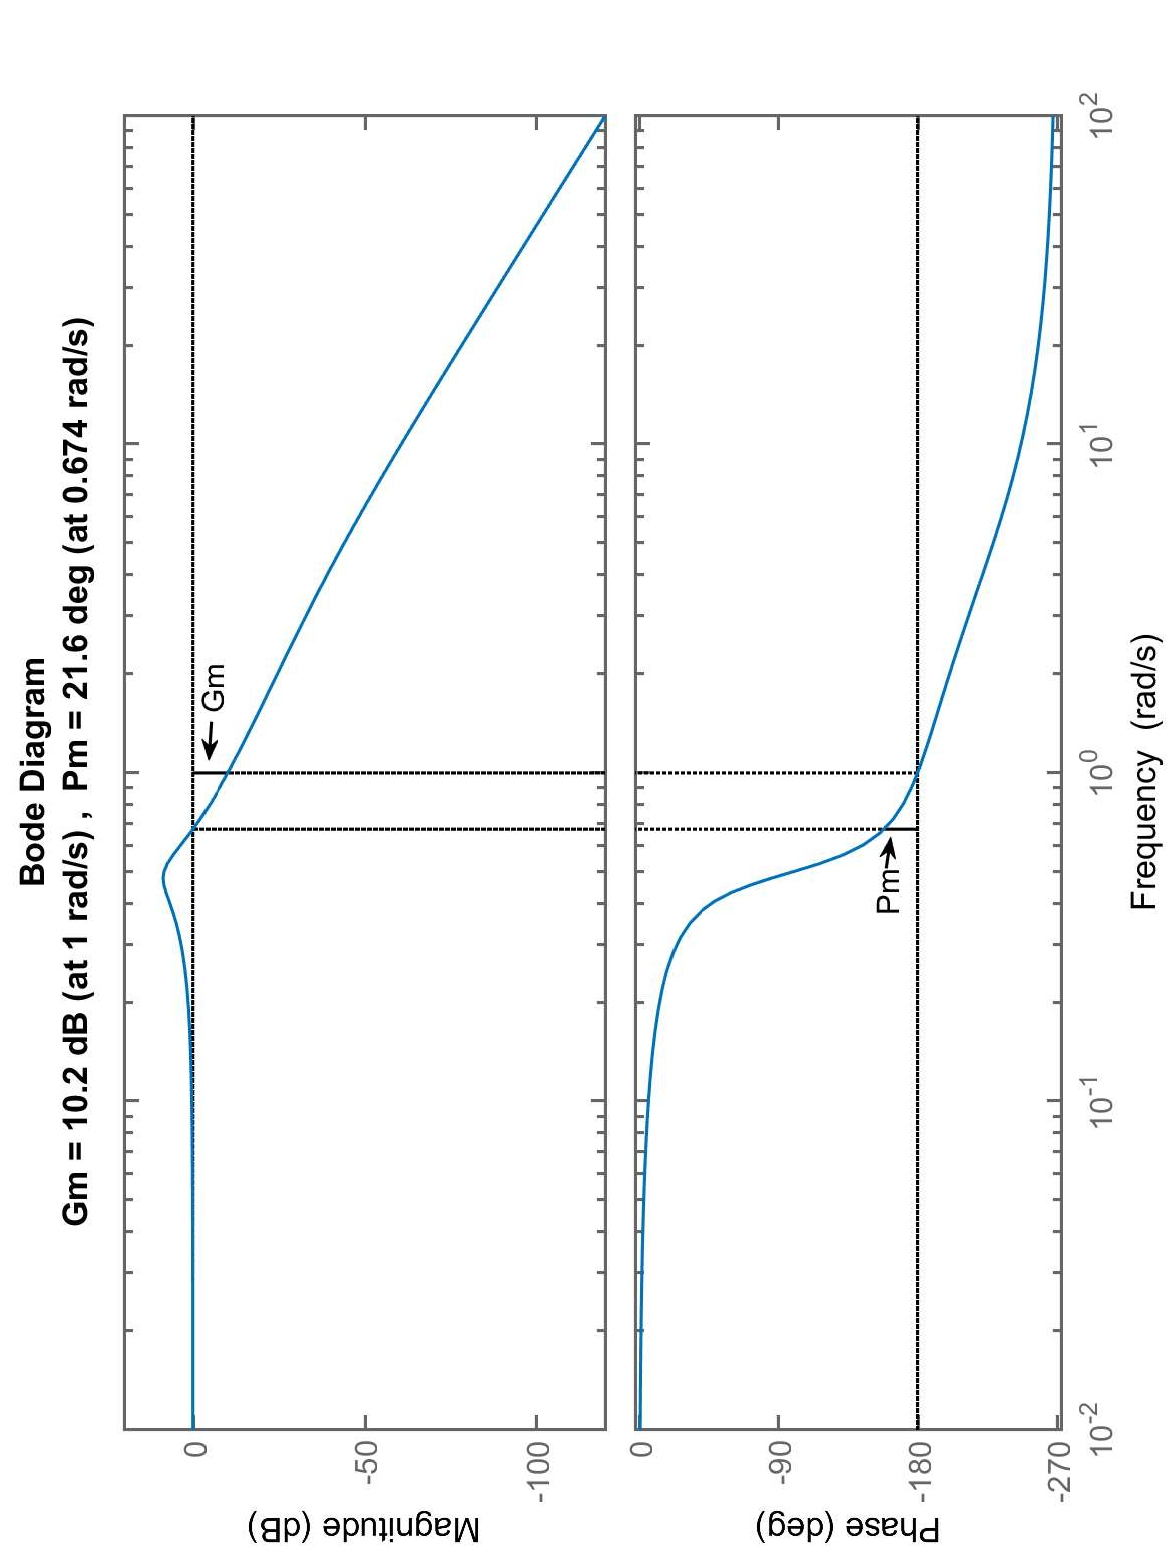
\includegraphics[width=0.6\textwidth, angle=-90]{figures/PM_GM.pdf}
\caption{Bodeplots of an open loop illustrating PM and GM.}
\label{fig:phaseGain}
\end{figure}
The phase margin is found by reading the angle velocity from the magnitude bode plot at gain = 0 dB, and finding the phase angle at this anglular velocity on the phase angle plot. The phase angle subtracted from $-180\degree$ yields the PM \citep{sou:MC}.

The gain margin is found by reading the angular velocity from the phase angle plot at the phase of $-180\degree$, and finding the gain at this angular velocity on the magnitude plot. The difference between this gain and unity gain (0 dB) is the gain margin.

From \autoref{fig:phaseGain}, it can be concluded that the phase margin is defined as how much additional phase shift it would take before the system becomes unstable. On the other hand, the gain margin describes how much the gain may change before the system becomes unstable.

In the beginning of this section, it was stated that the purpose with PM and GM is to keep uncertainties from making the system unstable. In this context, uncertainties being everything that causes the closed loop system to not behave ideally, such as circuit component sensitivity, delay caused by sampling etc. The scale of these inconsistencies is not yet know, so the exact influence these will have on the system cannot be determined. A rule of thumb regarding the PM and GM, states that PM should be greater than or equal to $45\degree$ whereas GM should be greater than or equal to 6 dB \citep{sou:PmGm}. However, to fulfill the time domain requirements, it is necessary to have $\zeta \geq 0.8$, which, based in \autoref{zeta}, results in a phase margin requirement of at least $80 \degree$.\\
From the above considerations, a list of specific requirements can now be set.

\section{List of Requirements \label{requirements}}
Based upon the previous considerations, requirements for the segway can be determined. The requirements are as follows:

\subsection*{Functional Requirements}
\begin{enumerate}
\item The segway must be able to stabilise itself in an upright equilibrium state.\label{funcReqBalance}
\item The segway must be able to drive forward and backwards without causing the segway to fall over.
\item The segway must be able to turn without causing the segway to fall over.
\item The segway may not fall over when pushed lightly.
\item The user must be able to make the segway drive by a wireless controller.
\item The user must be able to make the segway turn by a wireless controller.
\item The user must be able to receive data from the segway on a wireless controller.
\end{enumerate}
\subsection*{Performance Requirements}
The following requirements describes the desired performance of the segway. The first list of requirements is for the time domain, determining the dynamic behaviour of the segway. %Note that these requirements are made based on choices made by the project group and therefore chosen.
\begin{itemize}
\item Steady state error: 0 \%
\item Rise time: $\leq$ 1 s
\item Settling time: $\leq$ 3 s
\item Overshoot: $\leq$ 10 \% 
\end{itemize}
The following list describes the desired stability margins, i.e. the frequency domain requirements:
\begin{itemize}
\item Phase margin: $\geq 80\degree$
\item Gain margin: $\geq$ 6 dB
\end{itemize}

Now that the requirements are set, the development of the system can begin. This includes designing the controller which is to stabilize the system, together with a filter design and the design of the remote controller and the communication protocol. In the following section, a model of the system is derived, as this is needed to make a controller for the system.
%\begin{itemize}
%\item Rise time: TBD
%\item Settling time: TBD
%\item Overshoot: TBD
%\item Steady state error: TBD
%\item 
%
%\end{itemize}



%\section{Acceptance test description}
%Another title.\\

%\subsection{Performance requirements}
%Based on these principles requirements will be set as follows:
%\begin{enumerate}
%\item 
%\end{enumerate}
%
%\begin{enumerate}
%	\item Segway must be able to balance
%	\begin{itemize}
%		\item Rise time
%		\item Settling time
%		\item (Overshoot)
%		\item Phase margin - rule of thumb
%		\item Gain margin - rule of thumb
%	\end{itemize}
%	\item Segway must be able to drive
%	\begin{itemize}
%		\item Forward/Backward
%		\item Turning
%	\end{itemize}
%	\item It must be possible to remote control the segway wirelessly
%	\begin{itemize}
%		\item Zigbee
%		\item remote control drive elements
%	\end{itemize}
%	
%\end{enumerate}
\chapter{Sensors}
In this chapter, the setup of the sensors used by the segway is described. In a control system the sensors measure the output of the system, $Y$, and feed it back into the system as seen in \autoref{fig:modelBlockS}.

\begin{figure}[H]
\centering
\scalebox{0.8}{
\input{figures/modelBlock.poul}
}
\caption{Feedback loop of a system, with the sensor, $H$, highlighted.}
\label{fig:modelBlockS}
\end{figure}
A general feedback loop, see \autoref{fig:modelBlockS}, consists of three blocks. A controller, $D$, the system that is to be controlled, known as the plant, $G$, and sensors, $H$. The loop holds a reference signal, $R$, an error signal, $E$, the control signal, $U$, between the controller and the plant, and an output, $Y$. It is the sensor block, that is to be determined in this chapter, as highlighted in \autoref{fig:modelBlockS}.

In Section \ref{controlLoopOverview}, it was argued why the transfer function of the sensor block was set to be equal to 1, i.e. $H(s)=1$. Even though this is the case, the sensors used in the system still need to be described, so it is known which parameters of the system are measurable. This is also important to investigate since the way the data is obtained might influence the implementation of the controller.

The segway has four sensors that can be used to measure the speed, angular velocity and angle of the segway. To measure the speed, two encoders are available to measure the rotational velocity for both motors. The angle and angular velocity can be found from the gyroscope and the accelerometer. The structure of the following sections is to first describe the interface between the sensor hardware and the microcontroller (MCU) ATxmega128A3U and afterwards explain the implementation. %How the data is preprocessed is also described. The implementation is done on a ATxmega128A3U microprocessor. 

\section{Accelerometer and Gyroscope}
From \autoref{sec:hardware} it is known that the accelerometer and gyroscope are part of the MPU6050 transducer. This sensor has six degrees of motion, since both the accelerometer and gyroscope are 3-axis sensors. The accelerometer and gyroscope are used to derive the angle and angular velocity of the segway. To acquire the measured data from the sensors, the sensors have an \gls{I2C} bus, which can be interfaced to from the MCU.
  
\subsection{\iic Data}
The physical interface consists of two wires Serial Data (SDA) and Serial Clock (SCL). In normal mode the bus supports clock speeds up to 400 kHz, but additions can be made so the speed can go up to 5 MHz \citep{I2C}. In idle the voltage on the data line is pulled high. On a data level, a transmission consists of a start sequence, 7 bit address, R/W bit, acknowledge, followed by a start sequence, 8 data bit, acknowledge and a stop sequence. This can also be seen in \autoref{fig:I2CFrame}. Note that it is possible to transmit multiple data bytes without having to specify the address between each data transfer.

\begin{figure}[H]
\centering
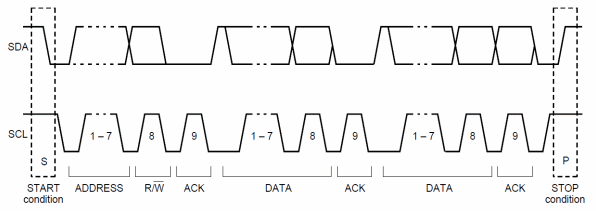
\includegraphics[width=\textwidth]{I2Cframe.png}
\caption{A visual representaion of a \gls{I2C} frame \citep{sou:i2c}.}
\label{fig:I2CFrame}
\end{figure}

\subsection{Data Acquisition from Gyroscope and Accelerometer}
The \gls{I2C} communication protocol is implemented in the MCU as a software module, since the pins, connected to pin 0 and 1 on port A, do not support hardware \gls{I2C}. The implemented \gls{I2C} driver, has been provided by group 15gr633, from AAU, who previously worked with the segway. From the header file, it can be seen that the library has 11 functions \autoref{lst:I2CFunctions}. From these functions the three functions i2cInit, i2cWrite and i2cRead are the main functions, the rest are subroutines that are called from the main functions.

\lstset{language=C, caption={Pre initialization of \gls{I2C} functions.}, label=lst:I2CFunctions}
\begin{lstlisting}
void i2cInit();
uint8_t i2cWrite(uint8_t slaveAddr, uint8_t regAddr, uint8_t *data, uint8_t length);
uint8_t i2cRead(uint8_t slaveAddr, uint8_t regAddr, int8_t *data, uint8_t length);

void i2cRepeatedStart(); 
void i2cStart();
void i2cStop();
void i2cTransmit(uint8_t data);
uint8_t i2cReceive();
uint8_t i2cGetAck();
uint8_t i2cSendAck();
uint8_t i2cSendNack();
\end{lstlisting}

From the datasheet it is known that the MPU6050 sensors \gls{I2C} address is 0x68 \citep[p. 46]{gyro}. When the sensor is powered on, it is in sleep mode. To wake up the sensor, 0x00 is written to the PWR\_MGMT\_1(Power Management 1) 8-bit register. Each sensor has six 8-bit registers for measured data. The three axes' values are sampled by three 16-bit ADC and then stored as MSB and LSB, giving six data registers for each sensor. From the datasheet it is known that the accelerometer data is stored in the registers from 0x3B to 0x40, while the gyroscope data is stored in the registers from 0x43 to 0x48. 

Note that both the gyroscope and the accelerometer work in polling mode, meaning that the current measurements are not sent automatically to the microcontroller, but will instead have to be requested over \gls{I2C}. The sensor modules takes care of obtaining the measurements and storing them in an internal register automatically - it is only the extraction of this data that is done in polling mode.

\subsection{Data Processing the Gyroscope and Accelerometer}
When the data is collected from the registers, they are put together to three 16 bit words. The accelerometer and gyroscope use the same coordinate system, but the orientation of this coordinate system (x, y, z) must be compared to the segway, which can be seen in \autoref{fig:sensor_orientation}. 

\begin{figure}[H]
\centering
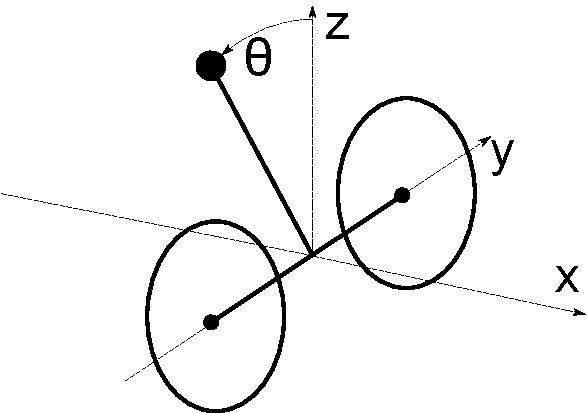
\includegraphics[width=0.4\textwidth]{figures/3D_seg_balance.pdf}
\caption{The sensors' orientation compared to the segway.}
\label{fig:sensor_orientation}
\end{figure}

To calculate the tilting angle of the pendulum, $\theta_p$, different methods can be used. For instance, the accelerometer can calculate the angle based on the direction of gravity, or by integrating the gyroscope data, which measures angular velocity. These methods have a couple of problems though. For instance, the accelerometer is very sensitive to changes in movement due to the acceleration applied. The gyroscope however, has a tendency to drift due to the integration \citep{IMU}. To obtain the angle it can therefore be advantageous to combine these measurements. This is done in a complementary filter \citep{IMU}, where measurements from both of the sensors are weighted and summed. 
\newpage
From \autoref{fig:sensor_orientation} it can be deducted that the pendulum angle can be calculated based on the accelerometer as: 
$$\theta_{pAx} = -\text{tan}^{-1}\left(\frac{x_{Ax}}{z_{Ax}}\right)$$ 
\begin{where}
\va{$\theta_{pAx}$}{is the angle of pendulum}{$\text{rad}$}\\
\va{$x_{Ax}$}{is the accelerometer measurement in the x-axis}{1}\\
\va{$z_{Ax}$}{is the accelerometer measurement in the z-axis}{1}\\
\end{where}

To get the angular velocity from the gyroscope, it is first recognised, based in \autoref{fig:sensor_orientation}, that it is the data in the y-axis, that is of interest. 
The angular velocity can then be calculated as follows:
\begin{equation}
\omega_p = \frac{y_{Gyro} \cdot max}{n}
\end{equation}
\begin{where}
	\va{$\omega_p$}{is the angular velocity of the pendulum}{rad/s}
	\va{$y_{Gyro}$}{is the data from the gyroscope in the y-axis}{1}
	\va{$max$}{is the gyroscope maximum measurement}{rad/s}
	\va{$n$}{is the number of digital representation for the gyroscope data}{1}
\end{where}

Using the complementary filter, the angle can be found as:

\begin{equation}
\theta_p = k \cdot \theta_{pAx} + (1-k) \cdot \int \!\omega_p \,\rm{d}x
\label{complementary}
\end{equation}

From \autoref{complementary}, it is seen how the angle is estimated from both accelerometer and integrated gyroscope data, and then the two values are weighted. The weighting factor $k$ is found experimentally to 0.05.
\newpage
\section{Encoder and Quadrature Decoder}

To determine the velocity of the wheels at a specified time, the exact change of position over an infinitesimal timespan shall be known, as the velocity $v(t)$ can be expressed by the time derivative of the position $s(t)$:
\begin{align}
v(t) = \frac{\text{d}s(t)}{\text{d}t}
\label{velocity}
\end{align}
\begin{where}
\va{$v(t)$}{is a function for velocity}{$\text{m/s}$}\\
\va{$s(t)$}{is a function for position}{$\text{m}$}\\
\end{where}

To determine a function for the position it is desired to decode the output signal from the encoders since they provide measurements about position changes over time. 

The encoders used for the segway are quadrature encoders. The output from a quadrature encoder is two square waves phase shifted by 90$\degree$ from two channels as illustrated in \autoref{fig:incremental_encoders2}. 

\begin{figure}[H]
	\centering
	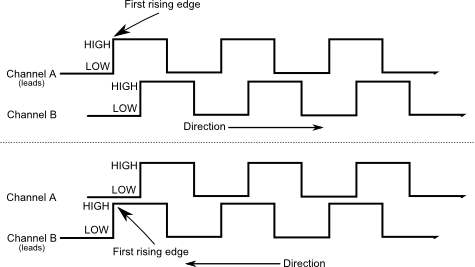
\includegraphics[width=0.7\textwidth]{figures/quad-encoding-waveform.png}
	\caption{Quadrature signal \citep{sou:quad_enc}.}
	\label{fig:incremental_encoders2}
\end{figure}

The signals from the encoders provide information about the direction and velocity of the wheel. Since the square waves from channel A and B are 90$\degree$ out of phase, the direction of the wheels can be found by determining the first rising edge of the signals from channel A and B. As the direction of the wheels change, the first rising edge will occur at the other channel.

The velocity can be determined by the number of of the square waves per time unit. One encoder rotation correspond to 512 high/low cycles or 2048 counts. A count is an event change in either channel A or B. E.g. if channel A goes low it will result in a count. The relation between the position and the number of counts is given by:

\begin{align}
s(t) = \frac{d \cdot \pi \cdot N_{ms} \cdot N_{sw}}{4\cdot CPR} \cdot c(t) \qquad \{c(t) \in \mathbb{Z}\}
\end{align}
\begin{where}
\va{$d$}{is the diameter of the wheel}{$\text{m}$}\\
\va{$N_{ms}$}{is the encoder/shaft ratio}{1}
\va{$N_{sw}$}{is the shaft/wheel ratio}{1}
\va{$c(t)$}{is number of counts. $c(t)$ can only be an integer.}{1}
\va{$CPR$}{number of cycles in one encoder rotation}{1}
\end{where}

The function $c(t)$ changes by the velocity of the wheels. Since $c(t)$ is an integer, the resolution of the position change is limited to the a-coefficient in the equation of $s(t)$, which is a linear expression on the form $s(t) = a \cdot c(t)$. The a-coefficient can be calculated by inserting the values given by the datasheets and measurements, see \autoref{app:segwayParameters} and \autoref{motorMeasReport}.
\begin{align}
s(t) = \frac{d \pi \cdot N_{ms} \cdot N_{sw}}{4\cdot CPR} \cdot c(t) \Rightarrow s(t) = \frac{0.117 \, \text{m} \cdot \pi \cdot  \frac{1}{19} \cdot \frac{25}{90}}{4\cdot 512} \cdot c(t) \approx 2.62 \cdot 10^{-6} \: \text{m} \cdot c(t)
\label{eq_st}
\end{align}

\autoref{eq_st} yields that 1 count is equal to $2.62 \cdot 10^{-6} \: \text{m}$. The expression of $s(t)$ from \autoref{eq_st} is inserted into \autoref{velocity}, yielding:
\begin{align}
v(t) = 2.62 \cdot 10^{-6} \: \text{m} \cdot \frac{\text{d}c(t)}{\text{d}t} \qquad \{c(t) \in \mathbb{Z}\}
\label{eq_vel}
\end{align}

Since the microcontroller responsible for measuring the encoder only works in discrete time, it is impossible to compute the derivative in \autoref{eq_vel}. Instead, a close approximation of \autoref{eq_vel} can be described as:
\begin{align}
v(t) \approx 2.62 \cdot 10^{-6} \: \text{m} \cdot \frac{c(t)-c(t_1)}{t-t_1} = 2.62 \cdot 10^{-6} \: \text{m} \cdot \frac{\Delta c(t)}{\Delta t}
\label{eq_vel2}
\end{align}

Whereas \autoref{eq_vel} gives the exact velocity of the wheels at a given time $t$, \autoref{eq_vel2} gives the approximated velocity in the time span $\Delta t$. This means the precision of the velocity is determined by $\Delta t$. A smaller time span $\Delta t$ gives a better precision.
If the time span $\Delta t$ is fixed, meaning $\Delta t$ is always set to 1 ms, the time span can known as the sampling period $T_{s}$. The inverse of $T_{s}$ is the sampling frequency $f_{s}$.
\begin{align}
v(t) \approx 2.62 \cdot 10^{-6} \: \text{m} \cdot f_s \cdot \Delta c(t) 
\end{align}

To get an accurate velocity, the sampling frequency is set to 1 kHz, but due to rounding in the frequency scaling in the MCU, this frequency cannot be obtained exactly. This small error is however disregarded.
\begin{align}
v(t) \approx 2.62 \cdot 10^{-6} \: \text{m} \cdot 1 \: \text{kHz} \cdot \Delta c(t)  = 2.62 \cdot 10^{-3} \: \frac{\text{m}}{\text{s}} \cdot \Delta c(t) 
\label{eq_vel3}
\end{align}

From this, the wheel angular velocity can also be found:
\begin{align}
\omega_w(t) = \frac{2\pi}{r_w}\cdot v(t) = 963 \cdot 10^{-6} \cdot \Delta c(t) \frac{\text{rad}}{\text{s}}
\end{align}	
The next step is to implement \autoref{eq_vel3} on the microcontroller.

\subsection{Quadrature Decoder Setup}
To process the data from the encoders, some decoders are needed. As stated previously, every event equals to a logical change from channel A or B from the encoders. Since the segway features two encoders, one encoder is connected to port C and another to port E. To allow event detection on the XMEGA, the registers associated with the quadrature decoding are set. The functions used for the setup of the quadrature decoders are seen in \autoref{lst:encoderFunctions}.

\lstset{language=C, caption={Pre-initialization of quadrature decoder functions.}, label=lst:encoderFunctions}
\begin{lstlisting}
void qdec_setup();			// Setup registers for the quadrature decoder
void en_interrupt();		// Enable interrupt
float motor_speed_left();	// Calculate and return the velocity of the left wheel
float motor_speed_right();
\end{lstlisting}

All registers associated with the quadrature decoders are set in the function qdec\_setup(), where the hardware for the decoder is set up. The XMEGA has external hardware that supports quadrature decoding. This means that the microprocessor does not directly need to handle the encoder itself, but only needs to read the data from the decoder through an interrupt service routine (ISR). After calling this function, a counter register will increment by one every time an event changes is occurring from channel A and B from both encoders. 

\subsection{Data Processing the Encoder Measurements}
As previously stated, the sampling frequency for the decoders are set to $f_s = 1$ kHz. To ensure a sampling every 1 ms, a timer is set to count up 1 ms and interrupts in order to sample the counter from the decoders. The interrupt service routine is seen in \autoref{lst:decoderISR}.

\lstset{language=C, caption={Interrupt Service Routine (ISR) for sampling the counters.}, label=lst:decoderISR}
\begin{lstlisting}
ISR(TCD1_OVF_vect){
	encoder_ccnt = TCC1.CNT;		// Get the value from port C counter register
	encoder_ecnt = TCE1.CNT;		// -||- port E
	TCE1.CNT = 0;					// Reset the counter register
	TCC1.CNT = 0;									
}
\end{lstlisting}
If the velocity of the wheels is required, the functions motor\_speed\_left() and motor\_speed\_right() are called. The functions then return the speed of the left and right wheel. This is done by converting the encoder counter to velocity using \autoref{eq_vel3}.
%\begin{equation}
%	\omega_w = 2 \cdot \pi \cdot f_s \cdot N_{ms} \cdot N_{sw} \cdot \frac{cnt}{4 \cdot res}
%\end{equation}
%\begin{where}
%\va{$\omega_w$}{is the angular velocity of the wheel}{rad/s}\\
%\va{$f_s$}{is the sampling frequency of the encoders}{Hz}\\
%\va{$N_{ms}$}{is the gearing ratio from the motor to the shaft}{1}\\
%\va{$N_{sw}$}{is the gearing ratio from the shaft to the wheel}{1}\\
%\va{cnt}{is the counted value for the specific encoder}{1/RPM}\\
%\va{res}{is the resolution of the encoders}{1/RPM}
%\end{where}

\section{PWM and H-bridge}
To control the DC-motors connected to the wheels, two H-bridges are used. By using H-bridges it is possible to control both the direction and the speed of the DC motors. For each H-bridge, the pins D2, IN1 and IN2 on the H-bridge are used for this purpose. By feeding D2 with a PWM signal, the velocity is changed by changing the duty cycle. A duty cycle of 100\% results in the motors going on full speed, whereas a duty cycle of 0\% results in no rotation. To determine the direction, either IN1 or IN2 should be pulled high. \\\\
The H-bridges' IN1 and IN2 pins are connected to the microcontroller's pin PC2 and PC3, and PE2 and PE3. The D2 pin is connected to PC1 and PE1 - these pins are set to be the PWM generating outputs in the MCU. The functions associated with PWM generation can be seen in \autoref{lst:pwmFunctions}.

\lstset{language=C, caption={Pre initialization of PWM generation functions.}, label=lst:pwmFunctions}
\begin{lstlisting}
void PWM_setup();
void PWM_left(int duty);
void PWM_right(int duty);
\end{lstlisting}

When generating a PWM signal, the resolution of the PWM signals are set to 256 counts, which is considered to be sufficient.\\
As the sensor block in the feedback loop, see \autoref{fig:modelBlockS}, is now known, the system model of the segway is to be derived in the following chapter. 


%\section{Controllers}

%\part{Design \& implementation}
\chapter{Modelling} \label{ch:modelling}
To make the segway able to balance in an upright position and be able to drive as well, it is necessary to have a model of the system, to understand how the system behaves from a physical and mathematical perspective. In this chapter, this model will be derived. A model is a mathematical description of the system's behaviour, in this case both the electrical and mechanical parts of the system.
This is needed to design a controller for the system. %The model will al be used for verifying the controller before it is implemented in the real system, and 
%From the model, the controllertype can be determinedm depending on the system type.
\begin{figure}[H]
\centering
\scalebox{0.8}{
\input{figures/modelBlock.rasmus}
}
\caption{Feedback loop of a system, with the plant, G, highlighted.}
\label{fig:modelBlock}
\end{figure}
\vspace{-0.8 cm}
Looking at a general feedback loop, see \autoref{fig:modelBlock}, it consists of three blocks. A controller, $D$, a plant that to be controlled, $G$, and sensors, $H$. The control loop also features a reference signal, $R$, an error signal, $E$, the control signal, $U$, between the controller and the plant, and an output, $Y$. It is the model of the plant, that is to be determined in this chapter, as highlighted in \autoref{fig:modelBlock}.
\section{Modelling overview \label{sec:modelover}}
The segway can be described as an inverted pendulum, the cart can be moved by a motorized two-wheeled system in order to stabilize the segway in an upright position. 
\begin{figure}[H]
\centering
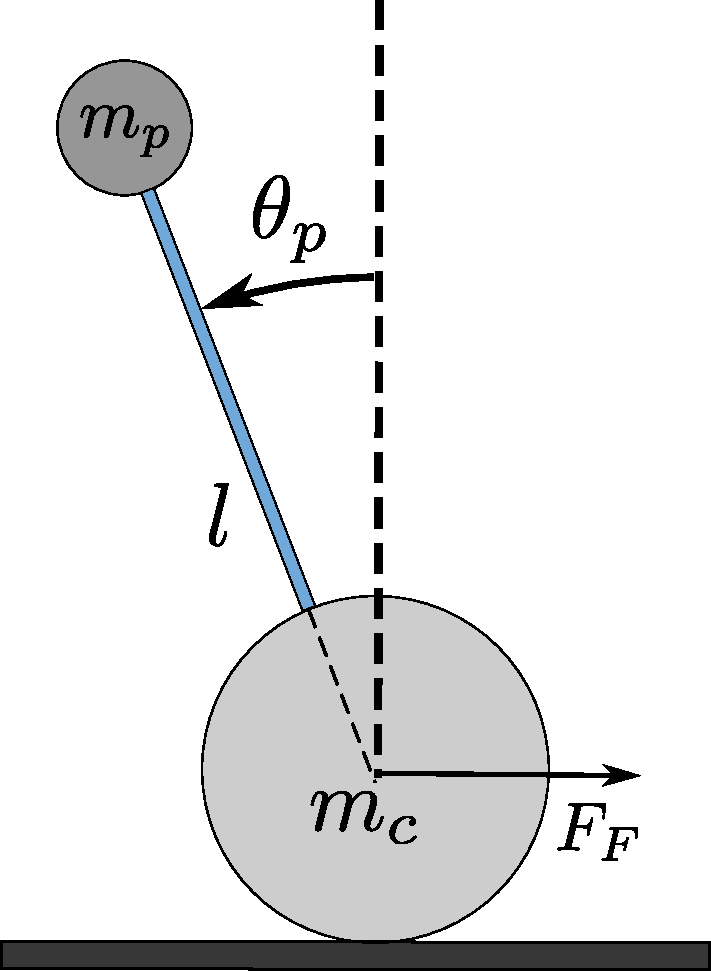
\includegraphics[width=0.25\textwidth]{/invertedPendulumModel.pdf}
\caption{An overall diagram of the segway.}
\label{fig:invertedPendulumModel}
\end{figure}
\vspace{-2em}
A figure of the segway with the cart mass, $m_c$, and inverted pendulum mass, $m_p$, can be seen in \autoref{fig:invertedPendulumModel}. Here, the inverted pendulum's tilting angle is represented by $\theta_p$, it can be further noted that the wheel's angle is denoted $\theta_w$.\\
The model of the segway is split in two smaller models, which is a model for the motor and wheel, and a model for the cart and inverted pendulum. These two models are later combined into a model for the segway. The splitting of the model can be seen in \autoref{fig:modelOverall}, together with the interfaces between the models.
\begin{figure}[H]
\centering
\input{figures/overallModel.rasmus}
\caption{The plant in the feedback loop. Within it is a motor and wheel model and a model for the inverted pendulum.}
\label{fig:modelOverall}
\end{figure}
\vspace{-2em}
The input to the system is the voltage applied to the motors, $V_a$. This voltage is controlled by simply changing the PWM duty cycle that controls the motors. In practice, this is equal to changing the motor input voltage. The interface signal between the motor and wheel model and the model describing the cart's movement is the torque applied by the motors to the cart, $\tau_a(t)$. Based on this torque, an expression for the force $F_F(t)$ can be made, which is the force that makes the segway move either forward or backwards.
The interface between the cart and the inverted pendulum is chosen to be the the angle of the wheels, $\theta_w$, as they determine the position of the segway. %This is the applied force to the segway, that makes it move. 
%The applied force, $F_F$,  is generated by the motors and wheels, and is what makes the segway move.\\
The model of the inverted pendulum has this angle, $\theta_w$ as input and the angle of the inverted pendulum, $\theta_p$, as output. Also, a load force $F_L(t)$ is inserted from the inverted pendulum to the cart model, as the tilting of the pendulum makes the cart move. % From the wheel angle, $\theta_w$, it is possible to set up an expression for the force that the wheels apply to the segway, named $F_F$, as this is used in the segway model.
%The reason why $F_F$ is chosen as the interface between the two smaller models is because it is usually such an input force that is used when modelling an inverted pendulum, see e.g. \citep{InvertedPendulumMathworks}. It will therefore be easy to put up a free body diagram of the inverted pendulum, since the contribution from the base to the pendulum is a force, easily included in the diagram.
\\\\
In this chapter, an expression for the motor and wheel model will be derived. Afterwards, a model of the cart and inverted pendulum is derived, see \autoref{fig:modelOverall}. These models will be simulated and verified, before being combined. Lastly the system model is simulated and verified. To be able to design a controller for the system, this model is then linearised and Laplace transformed to allow a transfer function to be derived, which is the final step performed in this chapter. %The transfer function of the system is the output of this chapter. \\
Firstly the motors and wheels model is to be derived in the following section. 
% From the model of the motors and wheels, a transfer function can be derived for the system. This transfer function can be be combined with a transfer function for the inverted pendulum, resulting in a transfer function for the entire plant.
%Thus the model transfer function can be described as a product of the partial system transfer functions:
%\begin{equation}
%G(s) = \frac{\theta_p(s)}{V_a(s)} = \frac{F_F(s)}{V_a(s)} \cdot \frac{\theta_p(s)}{F_F(s)}
%\label{eq:Gs_segway}
%\end{equation}
%
%\begin{where}
%\va{$G(s)$}{is the plant transfer function}{rad/V}
%\va{$V_a(s)$}{is the input voltage}{V}
%\va{$F_F(s)$}{is forward force}{N}
%\va{$\theta_p(s)$}{is the pendulum tilting angle}{rad}
%\end{where}
%\newpar
%Now that the model has been split up into two, each model will be separately derived. This is done in the following sections, starting with the motors and wheels model.
%The first step to create a control system for the segway is to model all the electrical and mechanical parts of the segway. The model determines how the segway behaves and can help to predict how it will react when a force or input is applied to different parts. The modelling of the segway is divided into two sections:% as seen on \autoref{fig:modelling_overview}.

%\begin{itemize}
%\item Modelling of the motors and wheels.
%\item Modelling of the inverted pendulum.
%\end{itemize}

%\begin{figure}[H]
%	\centering
%	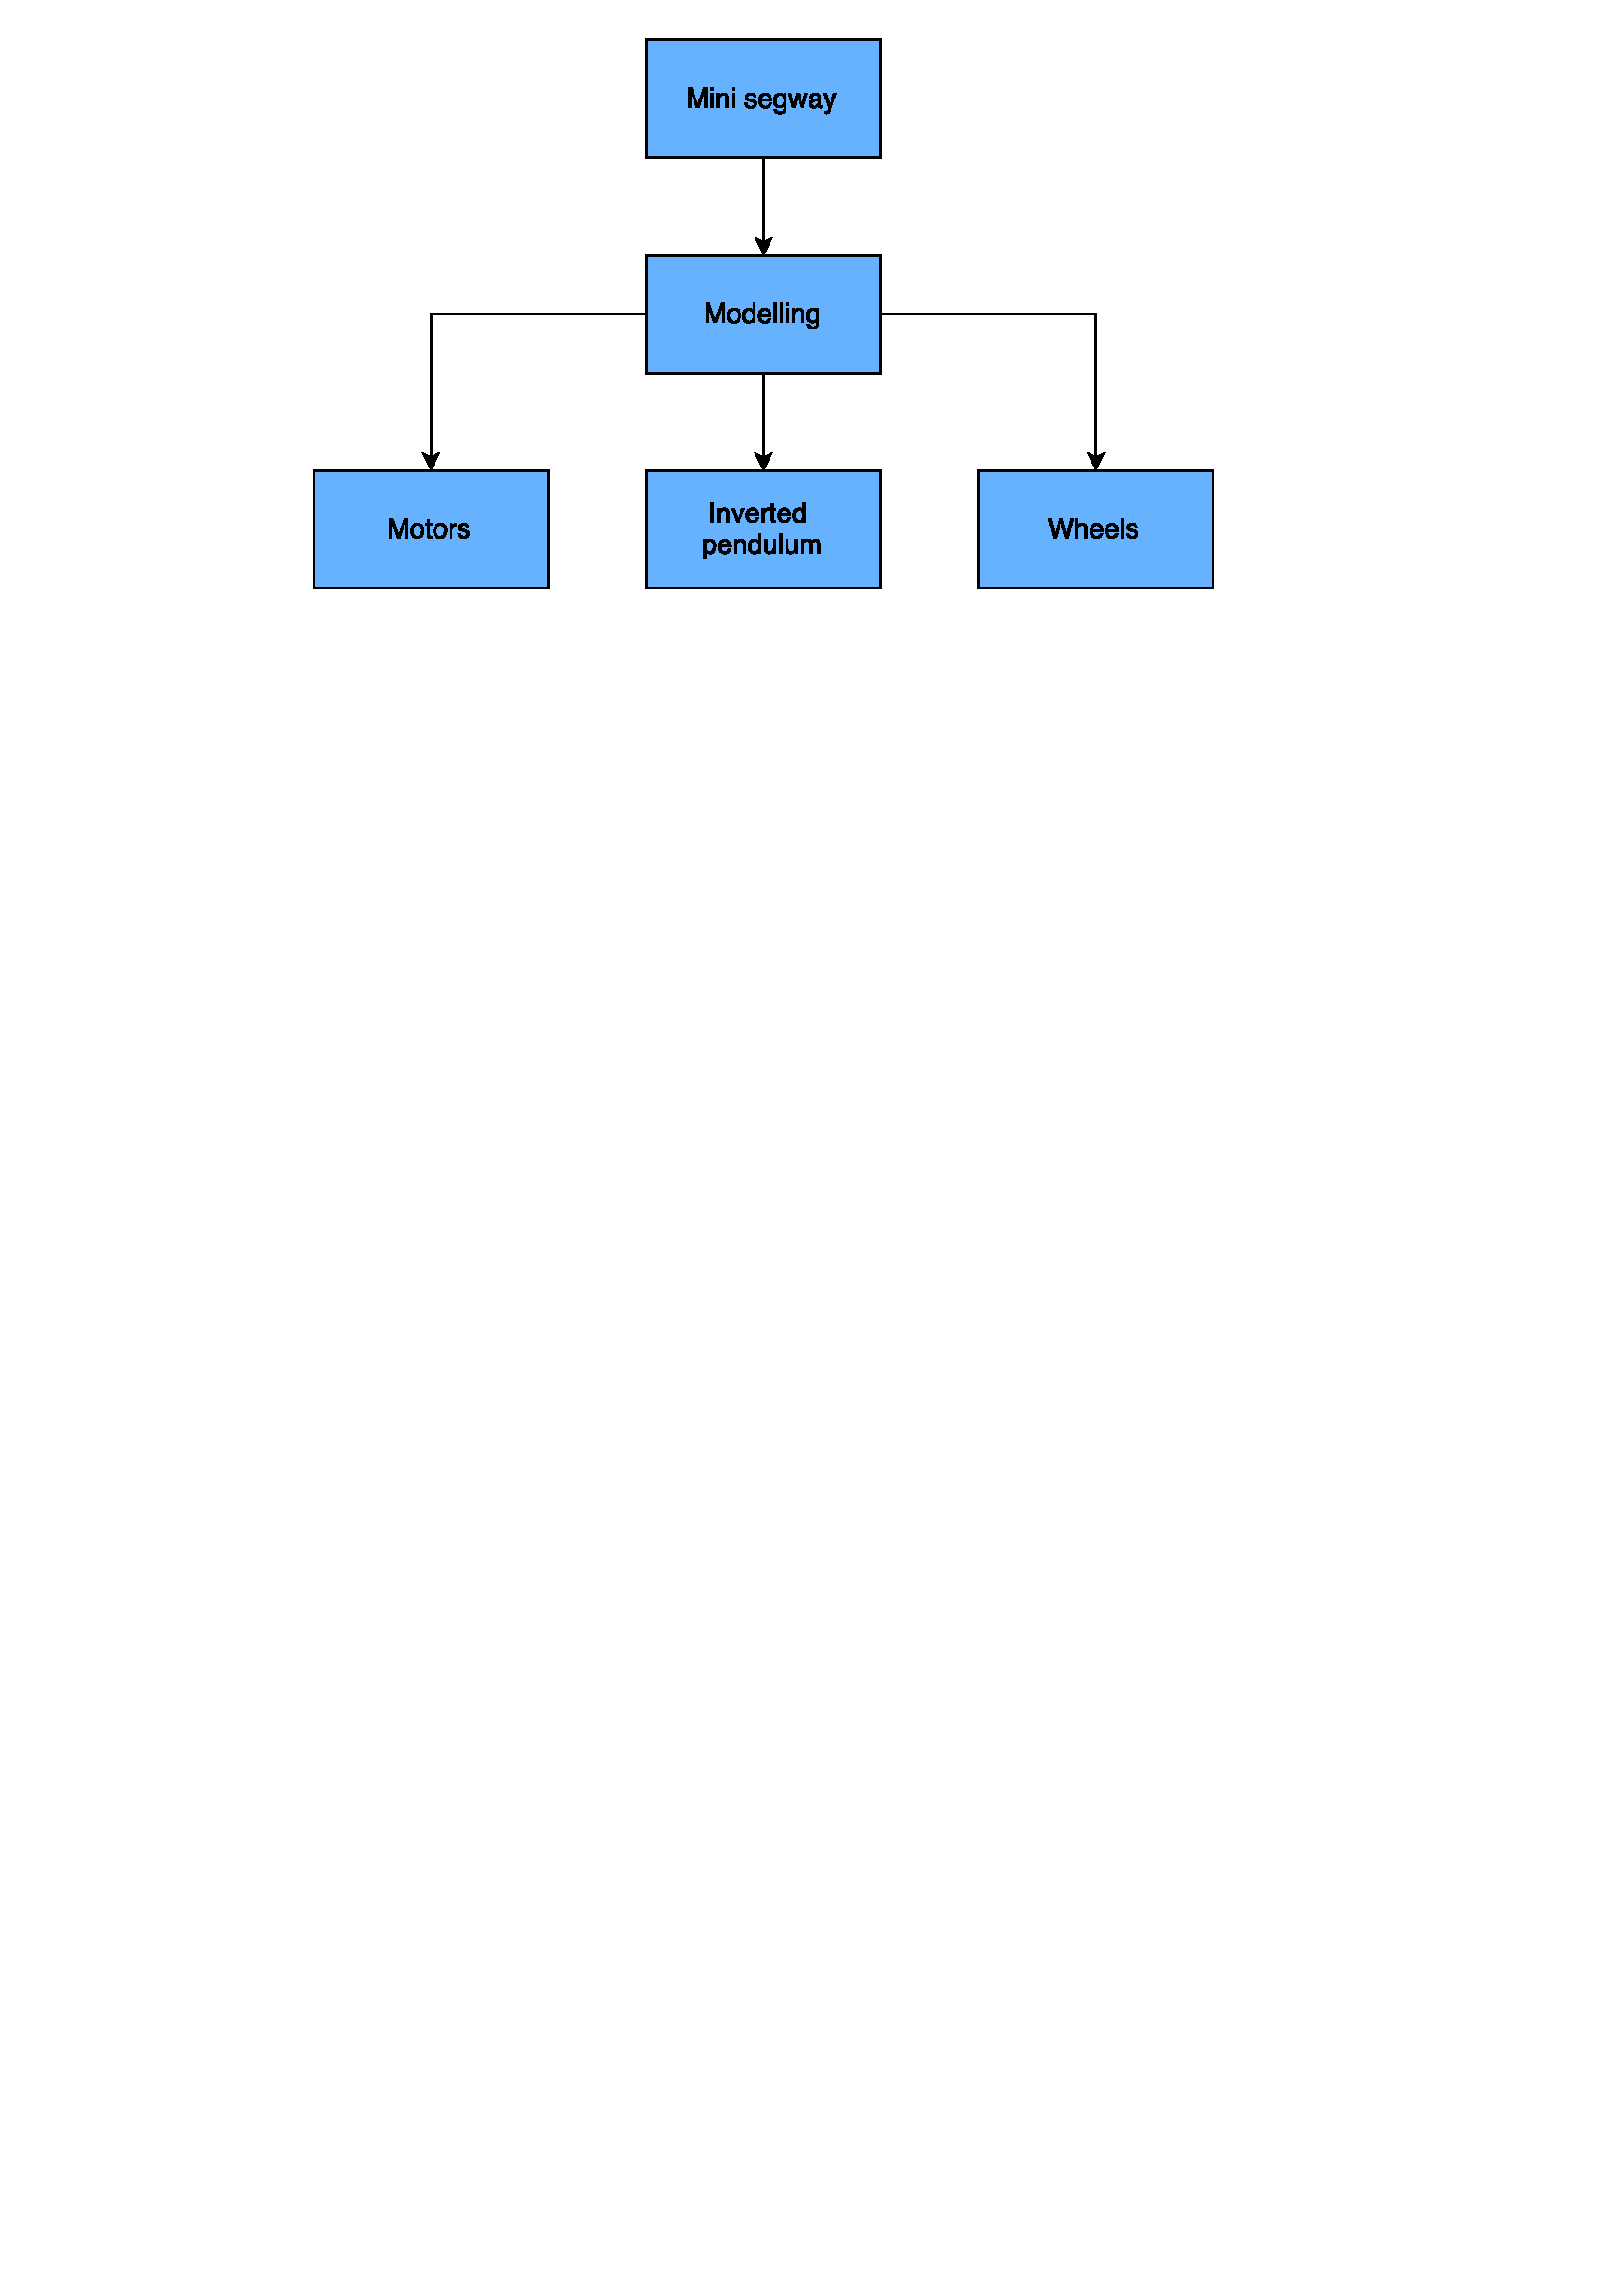
\includegraphics[width=0.7\textwidth]{design/figures/modelling/modelling_intro_block.pdf}
%	\caption{The division of the modelling.}
%	\label{fig:modelling_overview}
%\end{figure}

%The two sections are modelling of the inverted pendulum and modelling of the motors and wheels. The first part will consist of a modelling of the motors and wheels and the second part is the inverted pendulum. 

\section{Model of Motor and Wheel}
%An overall block diagram of the model of the motor and wheels can be seen on \autoref{fig:motorOverall}.
The model of the motors and wheels can be split into two parts; an electrical part and a mechanical part, since the two parts can be analyzed separately, though they are connected. This is due to the feedback that is present between the rotational velocity and the voltage, when modelling a motor \citep[15]{modelnote}.\\
The electrical model gives an output describing the motor current, $I_a(t)$. This is linked to the motor torque through the motor constant, $k_t$ \citep[p. 14]{modelnote}.\\
The mechanical part of the motor model describes both the motors, gears and wheels, since these are all connected. The mechanical part of the model has the angular velocity of the wheel, $\omega_w$ as output.
%A wheel model is also included to give the output of the motors and wheels model, that is the force applied, $F_F$, to the system by the motors and wheels.
A feedback is present in the system from $\omega_w$ to the applied voltage $v_a$, due to the back-EMF in the motor.\\
%\begin{figure}[H]
%\centering
%\scalebox{0.9}{
%\input{figures/overallMotor.rasmus}
%}
%\caption{An overall system diagram of the motor, gears and wheels.}
%\label{fig:motorOverall}
%\end{figure}
In the following, the electrical motor model is derived. Then, a mechanical model of the motors and wheels is put up. These two models can then be combined.\\
%\textbf{As the final step in the model of the motors and wheels, an expression for the applied force, $F_F$ is made, which can then be merged with the motor-wheel transfer function.}\\
Note that the modelling will be based on a single motor and wheel system, as the two motors and wheels on the segway are assumed identical. However, when deriving the expression for the applied force, $F_F$, both motors and wheels in the system are accounted for.
%After this, the inverted pendulum is modelled. This model can be combined with the motors and wheels model, to get the transfer function for the entire plant, as described in \autoref{fig:modelOverall}.\\
%In the following section, the electrical part of the motor is modelled.
\subsection{Electrical Motor Model}
The electrical part of a motor can be modelled using a resistor, $R_a$, an inductor, $L_a$, and a voltage generator, $V_e$, which delivers a voltage proportional to the motor's angular velocity $\omega_m$, also known as the back-EMF voltage \citep[p. 15]{modelnote}. This can be seen in \autoref{fig:motor_electrical}, where the input voltage, $V_a$, and the motor current, $I_a$, are shown, with the index $a$ denoting the armature of the motor. This model assumes that it is a permanent magnet DC motor that is used \citep[p. 15]{modelnote}, but as explained in section \ref{subsec:motors}, the motors used are of this type, meaning the model structure is valid.
\begin{figure}[H]
\centering
\begin{circuitikz}[american voltages]

	% electrical equivalent circuit
	\draw (0,0) to[V, v^=$V_a$] (0,3);
	\draw (0,3) to[R, i>^=$I_a$, l=$R_a$] (3,3);
	\draw (3,3) to[L, l=$L_a$] (4,3);

	\draw (4,3) -- (5,3);
	\draw (5,0) to[V, v_=\mbox{$V_e = k_e\omega_m$}] (5,3);
	\draw (0,0) -- (5,0);

\end{circuitikz}
\caption{Electrical curcuit equivalent of a DC motor.}
\label{fig:motor_electrical}
\end{figure}
Kirchoff's voltage law is applied to the circuit yielding the following expression:
\begin{equation}
0 = V_a(t) - R_a\cdot I_a(t) - L_a \dot{I_a}(t) - V_e(t) \label{eq:kirchoffsV}
\end{equation} 
\begin{where}
\va{$V_a(t)$}{is the motor input voltage}{V}
\va{$R_a$}{is the motor resistance}{$\Omega$}
\va{$L_a$}{is motor inductance}{H}
\va{$I_a(t)$}{is motor current}{A}
\va{$V_e(t)$}{is the back-EMF}{V}
\end{where}

%The equation is Laplace transformed to give the following:
%\begin{equation}
%\label{eq:electricMotor}
%0 = V_a(s) - R_a\cdot I_a(s) - s L_a I_a(s) - V_e(s)
%\end{equaeetion}

%$V_e$ is proportional to the motor velocity \citep[p. 15]{modelnote}, i.e.:
\clearpage
The back-EMF is directly proportional to the rotational speed of the motor:
\begin{equation}
V_e(t) = k_e \cdot\omega_m(t)
\end{equation}
\begin{where}
\va{$\omega_m(t)$}{is the rotational speed of the motor}{$\text{rad}/$s}
\va{$k_e$}{is the back-EMF constant}{V$/{\frac{\text{rad}}{s}}$}
\end{where}

Now, the expression for $V_e(t)$ can be inserted in \autoref{eq:kirchoffsV}. The equation is isolated for $I_a(t)$, since the current is the interface between the electrical and mechanical parts of the model. It is assumed that $\dot I_a(t) = 0$, since the electrical time constant is usually much higher than mechanical time constant \citep[p. 74]{sou:Feedback}. This yields \autoref{eq:electricMotor2}.
\begin{equation}
\label{eq:electricMotor2}
I_a(t) = \frac{1}{R_a} \left( V_a(t) - k_e \cdot \omega_m(t) \right)
\end{equation}
The torque of a motor is proportional to the current \citep[p. 14]{modelnote}:
\begin{equation}
\tau_m(t) = k_t \cdot I_a(t)
\label{eq:currenttau11}
\end{equation}
\begin{where}
\va{$\tau_m(t)$}{is the torque of the motor}{Nm}\\
\va{$k_t$}{is the motor constant}{Nm/A}\\
\end{where}

Inserting the expression for the current $I_a(t)$ from \autoref{eq:electricMotor2} into \autoref{eq:currenttau11} gives the following:
\begin{equation}
\label{eq:voltageToTorque}
\tau_m(t) = \frac{k_t}{R_a} \left( V_a(t) - k_e \omega_m(t) \right)
\end{equation}
%
%A block diagram of \autoref{eq:voltageToTorque} can be put up, see \autoref{fig:motorGearBlock}. Here, the input is the applied voltage $V_a(t)$, and the output the motor angular velocity, $\omega_m(t)$.
%
%Notice that a block describing the mechanical motor-wheel system has been inserted to transfer from torque, $t_m(t)$ to the angular velocity of the motor, $\omega_m(t)$. 
%%A gear transfer function is also inserted, to obtain the angular velocity of the wheel, $\omega_w(s)$ from the motor angular velocity, $\omega_m(s)$.
%
%\begin{figure}[H]
%\centering
%\input{figures/electricalMotor.rasmus}
%\caption{A block diagram of the motor and gearing.}
%\label{fig:motorGearBlock}
%\end{figure}

A model for the gears and wheel needs to be determined to find the torque $\tau_a$ that is applied to the segway, since the inertias and dampers in the gear-wheel setup influences this. This is done in the following section.
%In the next section, the transfer function for the mechanical system and the gears, describing the relationship between motor torque $\tau_m(s)$ and the rotational speed of the motor, $\omega_m(s)$, as well as the relationship between $\omega_m(s)$ and $\omega_w(s)$.

%In the feedback on \autoref{fig:motorGearBlock}, a transfer function describing the gearing is also needed, to describe the motor angular velocity $\omega_m(s)$ based on the wheel angular velocity, $\omega_w(s)$. These two gear transfer functions are derived in the following section. 
%To transfer from $\omega_w$ to $\omega_m$, the inverted gear ratio is inserted, since this is the connection between the two angular velocities.

%Ideally, the function in \autoref{eq:voltageToTorque} is turned into a transfer function describing the relationship between input voltage and motor torque. This is however not possible, since the gearing transfer functions are not yet known. Thus, these need to be determined before the transfer function for the system can be put up. 
%In the next section, the transfer function for the gears, describing the relationship between motor torque $\tau_m(s)$ and the rotational speed of the outer wheel, $\omega_w(s)$ can found. 
\subsection{Mechanical Motor and Wheel Model}
%The transfer function from motor torque $\tau_m$, to the angular velocity of the motor, $\omega_m$, is now to be found.
A model for the mechanical behaviour of the motors and wheels is to be found, so it can be combined with the electrical model for the motors, thus forming the combined model for the motors and wheels. \\
It is necessary to take the entire mechanical system, eg. both wheels and gearing ratios, into account, as these affect the motor's rotation.

\subsubsection{Gear relations}
First, the configuration of the gears are determined before the modelling can begin. The motor and wheel system consists of a DC motor, which has a gear mounted. The output of this gear is applied to the motor shaft, onto which a secondary gear is mounted. The inner wheel gear is mounted directly on the shaft, and thus has the same angular velocity as the motor. Therefore their inertia can be seen as one, being the shaft inertia. The configuration of the gears can be seen in \autoref{fig:gears}.
\begin{figure}[H]
\centering
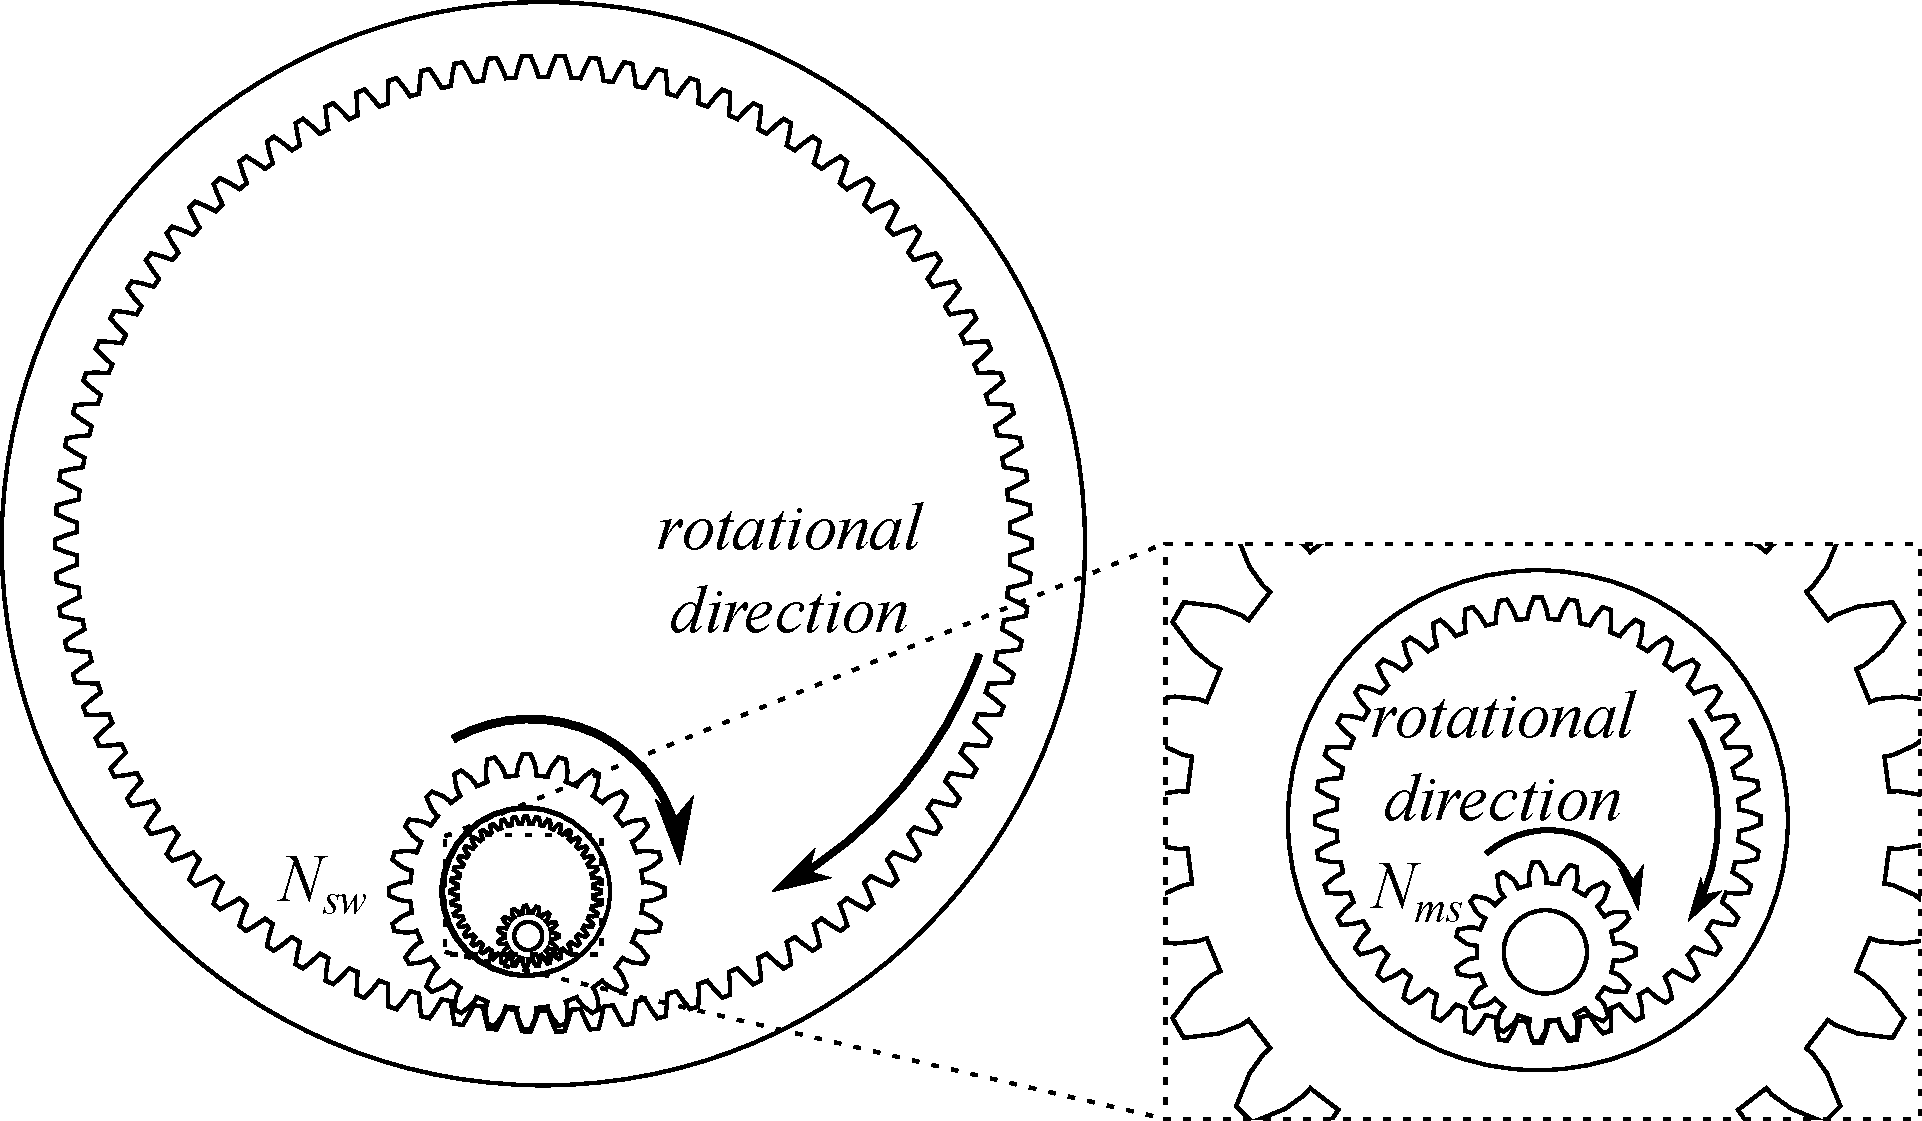
\includegraphics[width=0.75\textwidth]{figures/gears.pdf}
\caption{The different parts of the wheel's rotational system and its relative direction of rotation along with the gear ratios, $N_{ms}$ and $N_{sw}$.}
\label{fig:gears}
\end{figure}
In \autoref{fig:gears} the gear ratio between the motor and shaft is shown as $N_{ms}$, and the gear ratio for the shaft and wheel as $N_{sw}$.
\begin{figure}[H]
\centering
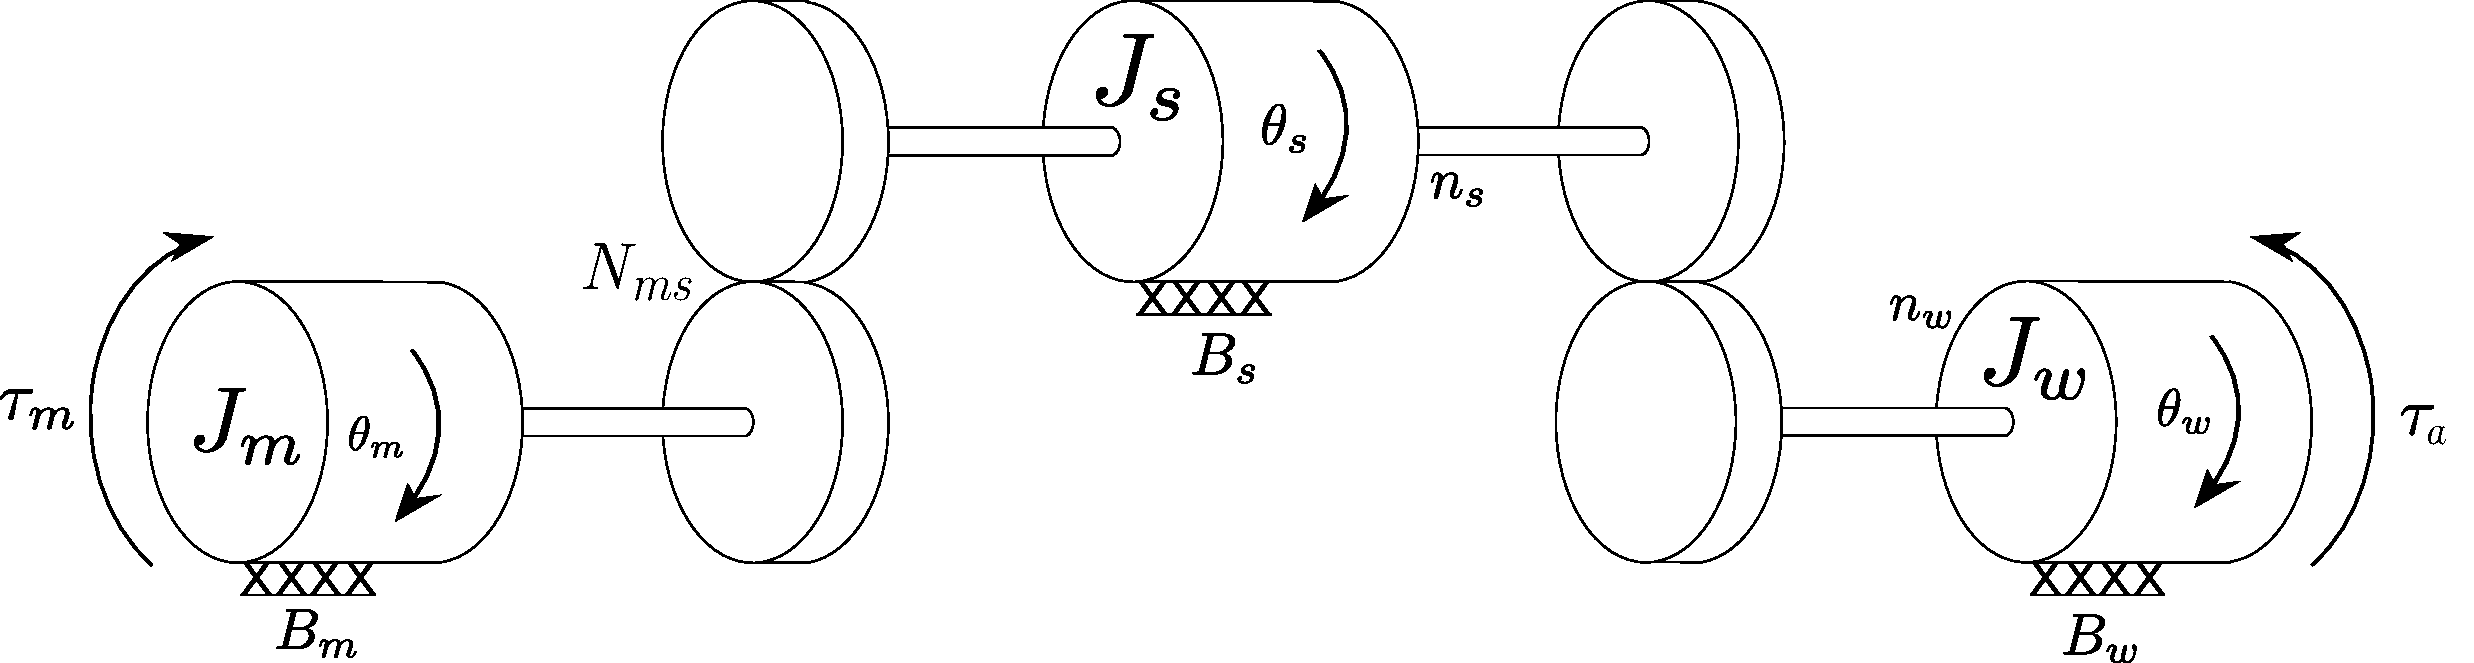
\includegraphics[width=\textwidth]{figures/motorRotationalDiagram.pdf}
\caption{Mechanical model of the motor and wheel setup.}
\label{fig:motorRotational}
\end{figure}

The gear ratio is used to determine the relation between angle and its derivatives for two or more rotational objects. The basis for determining is \autoref{fig:gearsRelation}, where it is assumed that there is no sliding between two gears. A torque $\tau_1$ is applied to the inner gear, giving it a certain angular position, $\theta_1$. The second gear also has a torque, $\tau_2$ and an angular position, $\tau_2$. Since the two gears have to move the same amount when rotating, as no slipping is assumed, \autoref{eq:gearRatio} can be put up, from which the gear ratio can be determined.

\begin{figure}[H]
\centering
\scalebox{1}{\input{figures/MotorAndWheel.ralf}}
\caption{Correlation of gears.}
\label{fig:gearsRelation}
\end{figure}

\begin{equation}
\theta_1r_1 = \theta_2r_2 \Rightarrow N = \frac{r_1}{r_2} = \frac{\theta_2}{\theta_1} = \frac{\omega_2}{\omega_1}
\label{eq:gearRatio}
\end{equation}
\begin{where}
\va{$N$}{The gear ratio}{1}
\va{$\theta_1$}{Angle of the inner gear}{rad}
\va{$\theta_2$}{Angle of the outer gear}{rad}
\va{$r_1$}{The radius of the inner gear}{m}
\va{$r_2$}{The radius of the outer gear}{m}
\va{$\omega_1$}{Angle velocity of the inner gear}{rad/s}
\va{$\omega_2$}{Angle velocity of the outer gear}{rad/s}
\end{where}

This, however, does not yield the relation between the torque of the gears and the gear ratio. This relation can be obtained through steady state analysis of each gear. This yields \autoref{eq:steadyGear1} and \autoref{eq:steadyGear2} for the inner and outer gear respectively, since the force of the two gears are of the same magnitude, i.e. $F_{g1}$ = $F_{g2}$ = $F_g$. This is because the force one gear excerts on the other is balanced by an equal, but opposite force, in correlation with Newton's 3rd law of motion. Based on this, it is possible to put up the following equations:
\begin{align}
\tau_1 - r_1\cdot F_g = 0 \label{eq:steadyGear1}
\\
\tau_2 - r_2\cdot F_g = 0\label{eq:steadyGear2}
\end{align}
\begin{where}
\va{$F_g$}{Translatoric force that works against the gear.}{N}
\end{where}

Thus, the gear ratio affects the relation between the torque in the two gears as shown in \autoref{eq:torqueRelation}.
\begin{equation}
\frac{\tau_1}{\tau_2} = \frac{r_1}{r_2} = N
\label{eq:torqueRelation}
\end{equation}

To describe the relation of the torque and the angle for two or more gears, the gear ratio, N, must be determined. This is done through the number of cogs in each cogwheel, as this can be thought of being equivalent to the wheel radii, which has previously been used to determine the gear ratio. From \autoref{subsec:wheels}, it's known that $n_s = 25$ and $n_w = 90$. From these, the gear ratio can be found.

\begin{equation}	
N_{sw} = \frac{n_s}{n_w} = \frac{\theta_w(t)}{\theta_s(t)} = \frac{25}{90} \approx 0.2778
\label{Nsw}
\end{equation}
\begin{where}
\va{$N_{sw}$}{is the shaft-wheel gear ratio}{1}\\
\va{$n_s$}{is number of cogs on the motor gear}{1}\\
\va{$n_w$}{is number of cogs on the wheel}{1}\\
\va{$\theta_s(t)$}{is the motor angle}{rad}\\
\va{$\theta_w(t)$}{is the wheel angle}{rad}\\
\end{where}

From \citep{gear} the gear ratio from motor to shaft is known:
\begin{equation}
N_{ms} = \frac{1}{19} \approx 0.053
\label{Nms}
\end{equation}
With the gear relations determined, it is now possible to derive the mechanical motor and wheel model.
\vspace{0.4 cm}
\subsubsection{Derivation of Mechanical Motor and Wheel Model}
\vspace{0.3 cm}
Now that the configuration of the rotational system is known, the motor, shaft and wheel system can be drawn using ideal elements, i.e. inertias and dampers, which can be seen in \autoref{fig:motorRotational}. Note, that all gears are assumed to have an inertia and a friction as no gears are assumed ideal. Also note that the friction in the gears is modelled as a damper, and thus each of the friction torques can be described in the same way as the friction torque for the shaft shown here: $\tau_{B_s}(t) = B_s \cdot \omega_s(t)$. The coulomb friction which is also present is not taken into account, due to the fact that an offset in the software can take care of this non-linearity, which is not easily modelled.\\
\clearpage
In \autoref{fig:motorRotational} it is seen how the motor connects to the shaft, which again connects to the wheel. All connections are made through gears. The constants $n_s$ and $n_w$, are the number of cogs on the shaft and wheel cog-wheels. These are used to determine the gear ratios.\newpar
The input torque to the motor $\tau_m(t)$, see \autoref{fig:motorRotational}, sets the direction of all the resultant angular positions, and therefore also angular velocities and angular accelerations in accordance with \autoref{fig:gears}.\\
The free body diagrams of the motor, shaft and wheel are illustrated in \autoref{fig:FBDMotorShaftWheel}. %In the motor part \autoref{fig:FBDMotor}, the motor torque, $\tau_m$, is inserted along with a friction torque, $\tau_{B_m}$, and a gearing torque transferring torque to the wheel.
%In the wheel part \autoref{fig:FBDWheel}, the gear torque, $\tau_{G_w}$, is inserted, along with a friction torque. The resultant torques are also shown.
\begin{figure}[H]
\centering
\begin{subfigure}[b]{0.3\textwidth}		
        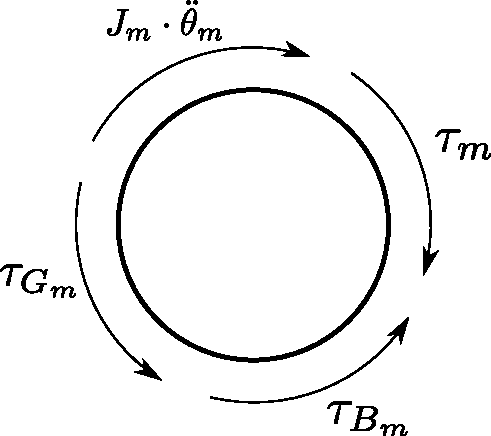
\includegraphics[width=0.98\textwidth]{figures/FBD/FBDMotor.pdf}
        \vspace{3.5mm}
        \caption{FBD of rotational system for the motor.}
        \label{fig:FBDMotor}
    \end{subfigure} 
    \hspace{4mm} 
\begin{subfigure}[b]{0.3\textwidth}
        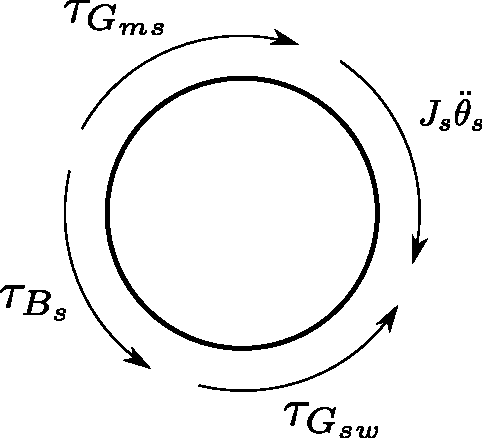
\includegraphics[width=0.95\textwidth]{figures/FBD/FBDShaft.pdf}
        \vspace{2mm}
        \caption{FBD of rotational system for the shaft.}
        \label{fig:FBDshaft}
    \end{subfigure}  
    \hspace{4mm} 
\begin{subfigure}[b]{0.3\textwidth}
        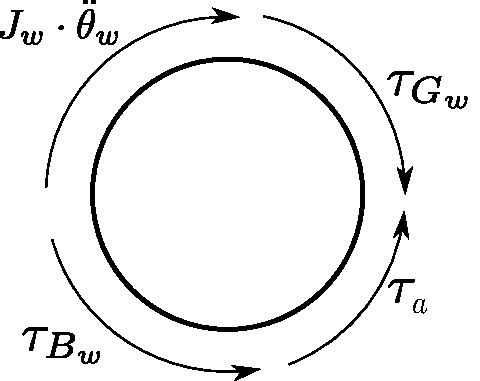
\includegraphics[width=0.95\textwidth]{figures/FBD/FBDWheel.pdf}
        \vspace{5mm}
        \caption{FBD of rotational system for the wheel.}
        \label{fig:FBDWheel}
    \end{subfigure}
\caption{Free body diagrams of the three rotational systems.}
\label{fig:FBDMotorShaftWheel}
\end{figure}
Note that the following relationships between the gear torques exist, based on the gear ratios: 
\begin{equation}
\tau_{G_{ms}}(t) = \tau_{G_m}(t) \cdot \frac{1}{N_{ms}}
\label{gearTorqueMotor}
\end{equation}
\begin{equation}
\tau_{G_w}(t) = \tau_{G_{sw}}(t) \cdot \frac{1}{N_{sw}}
\label{gearTorqueWheel}
\end{equation}
\begin{where}
\va{$\tau_{G_{ms}}(t)$}{is the torque from motor to shaft}{Nm}\\
\va{$\tau_{G_m}(t)$}{is the torque to shaft from motor}{Nm}\\
\va{$\tau_{G_w}(t)$}{is the torque from shaft to wheel}{Nm}\\
\va{$\tau_{G_{sw}}(t)$}{is the torque to wheel from shaft}{Nm}\\
\end{where}

From \autoref{fig:FBDMotorShaftWheel}, the following differential equations can be put up:
\begin{align}
J_m\ddot\theta_m(t) &= \tau_m(t) -\tau_{G_m}(t) - \tau_{B_m}(t)\label{eq:DE1}\\
J_s\ddot\theta_s(t) &= \tau_{G_{ms}}(t) - \tau_{G_{sw}}(t) - \tau_{B_s}(t)\label{eq:DE2}\\
J_w\ddot\theta_w(t) &= \tau_{G_{w}}(t) - \tau_{B_w}(t) -\tau_a(t) \label{eq:DE3}
\end{align}

\begin{where}
\va{$J_m$}{is the motor moment of inertia}{$\text{kg} \cdot \text{m}^2$}\\
\va{$J_s$}{is the shaft moment of inertia}{$\text{kg} \cdot \text{m}^2$}
\va{$J_w$}{is the wheel moment of inertia}{$\text{kg} \cdot \text{m}^2$}
\va{$\ddot\theta_m(t)$}{is the angular acceleration of the motor}{$\text{rad}/\text{s}^2$}\\
\va{$\ddot\theta_s(t)$}{is the angular acceleration of the shaft}{$\text{rad}/\text{s}^2$}\\
\va{$\ddot\theta_w(t)$}{is the angular acceleration of the wheel}{$\text{rad}/\text{s}^2$}\\
\va{$\tau_m(t)$}{is the delivered torque from the motor}{$\text{rad}/\text{s}^2$}\\
\va{$\tau_{B_m}(t)$}{is the motor friction torque}{Nm}\\
\va{$\tau_{B_s}(t)$}{is the shaft friction torque}{Nm}\\
\va{$\tau_{B_w}(t)$}{is the wheel friction torque}{Nm}\\
\va{$\tau_{a}(t)$}{is the torque applied to the cart}{Nm}\\
\end{where}

In the following, a model for the motors and wheels system is obtained. This is done using the differential equations derived from the free body diagrams, see \autoref{eq:DE1}, \autoref{eq:DE2} and \autoref{eq:DE3}.
%\textbf{In the following, a transfer function for the gearing/wheel system is obtained. The input to the system is the motor torque, $\tau_m(t)$, and the output is the angular velocity of the wheel, $\omega_w(t)$.
%This is done using the differential equations derived from the free body diagrams, see \autoref{eq:DE1}, \autoref{eq:DE2} and \autoref{eq:DE3}. It is desired to combine these equations, to obtain a transfer function for the entire mechanical model.\todo{not looking for a transferfunction. Rewrite}}
\\The model is derived by working from the outside and in, starting with the equations for the wheel and inserting them to get an expression for the motor that includes the wheel and shaft.\\
The differential equation for the wheel rotational system, \autoref{eq:DE3}, states:
\begin{equation}
J_w\ddot\theta_w(t) = \tau_{G_{w}}(t) - \tau_{B_w}(t) - \tau_a(t) \nonumber
\end{equation}
The linear approximation of the friction torque, which is modelled as a damper, can be described as $\tau_{B_s}(t) = B_s \cdot \dot\theta_s(t)$. Inserting this together with the expression for the gear torque from \autoref{gearTorqueWheel} gives:
\begin{equation}
J_w \ddot\theta_s(t) N_{sw} = \tau_{G_{sw}}(t)\cdot \frac{1}{N_{sw}} - {B_{w}} N_{sw} \cdot \dot\theta_{s}(t) -\tau_{a}(t)
\end{equation}
%Laplace transforming the equation and isolating for $\tau_{G_{sw}}$ gives:
%\begin{equation}
%s^2 J_w N_{sw} \theta_s(s) = \tau_{G_{sw}}(s)\cdot \frac{1}{N_{sw}} - s {B_{w}} N_{sw} \cdot \theta_{s}(s)
%\end{equation}
%\begin{equation}
%\tau_{G_{sw}}(s) = \theta_s(s) \cdot N_{sw}^2 (s^2 J_w + s B_w) 
%\label{tauGSW}
%\end{equation}
Isolating for $\tau_{G_{sw}}$ gives:
\begin{equation}
\tau_{G_{sw}}(t) = J_w \ddot\theta_s(t) N_{sw}^2 + B_wN_{sw}^2\dot\theta_s(t) + \tau_a(t) \cdot N_{sw}
\label{tauGSW}
\end{equation}
Now that an expression for $\tau_{G_{sw}}(t)$ is obtained, it can be combined with the differential equation for the second rotational system, \autoref{eq:DE3}, which states:
\begin{equation}
J_s\ddot\theta_s(t) = \tau_{G_{ms}}(t) - \tau_{G_{sw}}(t) - \tau_{B_s}(t) \nonumber
\end{equation}
The friction can, as previously mention be described as $\tau_{B_s}(t) = B_s \cdot \dot\theta_s(t)$. Inserting this and isolating for $\tau_{G_{ms}}(t)$ yields:
\begin{equation}
\tau_{G_{ms}}(t) = \tau_{G_{sw}}(t) + B_s \cdot \dot\theta_s(t) + J_s\ddot\theta_s(t) 
\label{tauGSAlmost}
\end{equation}
\autoref{tauGSW} is inserted in \autoref{tauGSAlmost} together with the expression for the motor-shaft gear from \autoref{gearTorqueMotor}. An expression for $\tau_{G_m}(t)$ can thus be found:
%\begin{equation}
%\tau_{G_{ms}}(t) = \left(J_w \ddot\theta_s(t) N_{sw}^2 + B_wN_{sw}^2\dot\theta_s(t) + \tau_a(t)\right) + B_s \cdot \dot\theta_s(t) + J_s\ddot\theta_s(t) 
%\label{tauGS}
%\end{equation}
%Inserting the motor-shaft gear ratio, an expression for $\tau_{G_m}(t)$ can be obtained:
%\begin{equation}
%\tau_{G_{m}}(s)\frac{1}{N_{ms}} = \theta_m(s){N_{ms}}(s^2(J_s + N_{sw}^2 J_w) + s (B_s + N_{sw}^2 B_w))\label{tauGMAlmost}
%\end{equation}
\begin{equation}
\tau_{G_{m}}(t) = J_w \ddot\theta_m(t) N_{ms}^2 N_{sw}^2 + B_w N_{ms}^2 N_{sw}^2\dot\theta_m(t) + \tau_a(t)\cdot N_{ms} N_{sw} + B_s N_{ms}^2 \cdot \dot\theta_m(t) + J_s N_{ms}^2 \ddot\theta_m(t) 
\label{tauGM}
\end{equation}

This expression can be combined with the differential equation for the motor rotational system, as seen in \autoref{eq:DE1} and stated here:
\begin{equation}
J_m\ddot\theta_m(t) = \tau_m(t) -\tau_{G_m}(t) - \tau_{B_m}(t) \nonumber
\end{equation}
Inserting the expression for the friction torque, $\tau_{B_m}(t) = B_m \cdot \dot\theta_m(t)$ and $\tau_{G_{m}}(t)$ as found in \autoref{tauGM} yields \autoref{eq:tauM(t)} where the motor torque $\tau_m(s)$ has also been isolated:\vspace{0.3 cm}
%\begin{equation}
%s^2 J_m \theta_m(s) = \tau_m(s) - \tau_{G_{m}}(s) - s{B_m}\theta_m(s)
%\end{equation}
%
%The motor torque, $\tau_m(s)$ is isolated:
\begin{align}
\begin{split}
\tau_m(t) = &J_m\ddot\theta_m(t) + B_m \cdot \dot\theta_m(t)+ ( J_w \ddot\theta_m(t) N_{ms}^2 N_{sw}^2 + \\ & B_w N_{ms}^2 N_{sw}^2\dot\theta_m(t) + \tau_a(t)\cdot N_{ms} N_{sw} + B_s N_{ms}^2 \cdot \dot\theta_m(t) + J_s N_{ms}^2 \ddot\theta_m(t) )
\end{split}
\label{eq:tauM(t)}
\end{align}
This simplifies to:
\begin{align}
\begin{split}
\tau_m(t) = &\ddot\theta_m(t)\left(J_m + N_{ms}^2(J_s  + J_w N_{sw}^2) \right) + \dot\theta_m(t)\left(B_m + N_{ms}^2(B_s + N_{sw}^2 B_w)\right) + \tau_a(t)\cdot N_{ms} N_{sw}
\end{split}
\label{eq:tauM(t)2}
\end{align}
To simplify the expressions, the following definitions are made for the total equivalent inertia, $J_T$ and the total equivalent friction, $B_T$:
\begin{align}
J_{T} &\equiv J_m + N_{ms}^2(J_s + N_{sw}^2 J_w)\label{TotalInertia}\\
B_{T} &\equiv B_m + N_{ms}^2(B_s + N_{sw}^2 B_w)\label{TotalDamper}
\end{align}

This means that the expression can be written as:
\begin{align}
\begin{split}
\tau_m(t) = &\ddot\theta_m(t)\cdot J_T + \dot\theta_m(t) \cdot B_T + \tau_a(t)\cdot N_{ms} N_{sw}
\end{split}
\label{eq:tauM(t)3}
\end{align}
Using this and inserting the motor torque, \autoref{eq:voltageToTorque}, and isolating for $\tau_a(t)$ yields:
\begin{equation}
\tau_a(t) = \frac{1}{N_{ms} N_{sw}}\left(\frac{k_t}{R_A} \left( V_a(t) - k_e \dot\theta_m(t) \right) - \ddot\theta_m(t)J_{T} - \dot\theta_m(t)B_{T}\right) 
\label{eq:MotorFinal}
\end{equation}
\autoref{eq:MotorFinal} is the final model expression for the motors and wheels part of the system. Now the model of the inverted pendulum is to be found. These model expressions are then to be combined. From this a controller can be designed and later implemented. The deriviation of the inverted pendulum model is done in the following section. 
%
%
%%
%%Using the gear ratios, an expression for the wheel position, $\theta_w(s)$ is obtained:
%%\begin{equation}
%%\tau_m(s) = \theta_w(s) \frac{s^2 (J_m + N_{ms}^2(J_s + N_{sw}^2 J_w)) + s (B_m + N_{ms}^2(B_s + N_{sw}^2 B_w)) }{N_{ms} N_{sw}}
%%\end{equation}
%
%\subsection{Combined motors and wheels model}
%In the following section, the electrical motor model is combined with the mechanical model, to derive an expression for the transfer function $\frac{F_F(s)}{V_a(s)}$.
%
%First, the an expression for the angular velocity of the wheel, $\omega_w$ needs to be derived, based on the angular velocity of the motor, $\omega_m$. This relationship is quite simple, as it is defined by the gear ratios, as can be seen in \autoref{Nsw}. Since there are two gears, the motor-shaft gear and the shaft-wheel gear, both of these gear ratios needs to be included. Thus, the transfer function for the two gears become:
%\begin{equation}
%\frac{\omega_w(s)}{\omega_m(s)} = N_{ms} N_{sw}
%\label{omegaTF}
%\end{equation}
%
%The translational force caused by a rotational system can be described as: 
%\begin{align*}
%F_F &= 2 m_w \cdot a_w \\
%&= 2 m_w\cdot r_w\alpha_w \\
%&= 2 m_w\cdot r_w \dot\omega_w
%\end{align*}
%\todo{maybe use mass of cart instead of wheel}
%\begin{where}
%\va{$F_F$}{is the resultant applied force of the wheels}{N}\\
%\va{$m_w$}{is the mass of the wheel}{kg}\\
%\va{$a_w$}{is translatoric acceleration of the wheel}{m/$\text{s}^2$}\\
%\va{$r_w$}{is the radius of the wheel}{m}\\
%\va{$\alpha_w$}{is angular acceleration of the wheel}{rad/$\text{s}^2$}\\
%\va{$\omega_w$}{is the angular velocity of the wheel}{rad/$\text{s}^2$}\\
%\end{where}
%
%The reason why a factor of 2 has been multiplied with the expression is because there are two wheels, each exerting their own applied force. The combined force is therefore the sum of these, which is the same as multiplying with two if the forces are assumed identical. 
%
%The transfer function from rotational speed of the wheel, $\omega_2$ to the force $F_F$ can thus be described as:
%\begin{equation}
%\frac{\F_F(s)}{\omega_w(s)} = 2 s r_w m_w
%\label{OmegaToForce} 
%\end{equation}
%
%It is now possible to combine the equations for the electrical system with the equations for the mechanical system:
%
%The transfer function $\frac{\omega_m(s)}{\tau_m(s)}$ can be inserted in \autoref{fig:motorGearBlock} in the mechanic system block. Also, the transfer functions $\frac{omega_w(s)}{\omega_m(s)}$ and $\frac{F_F(s)}{\omega_w(s)}$ from \autoref{omegaTF} and \autoref{OmegaToForce} can be inserted in the block diagram to obtain the force $F_F(s)$ as output. This can be seen in \autoref{fig:electricroMechanical}.
%
%\begin{figure}[H]
%\centering
%\scalebox{0.87}{
%\centering
%\input{figures/electromechanical.rasmus}
%}
%\caption{A block diagram of the mechanical system consisting of the motor, gear and wheels.}
%\label{fig:electricroMechanical}
%\end{figure}
%
%From this block diagram, the transfer function $\frac{\omega_w(s)}{V_a(s)}$ can be obtained, using the rules for blocks in serial and the rules for calculating feedback terms:
%\begin{equation}
%\frac{\omega_w(s)}{V_a(s)} = \frac{ \frac{k_t N_{ms} N_{sw}}{L_a J_T}}{s^2 + s\left( \frac{L_a B_T + R_a J_T}{L_a J_T} \right) + \frac{R_a B_T + K_t k_e}{L_a J_T}}
%\label{TF:motorWheelOmega}
%\end{equation}
%\begin{where}
%\va{$\omega_w(s)$}{is the wheel angular velocity}{rad/s}
%\va{$V_a(s)$}{is input voltage to the motor}{V}
%\va{$K_t$}{is the motor constant}{Nm/A}
%\va{$K_e$}{is the back-EMF constant}{V$/{\frac{\text{rad}}{s}}$}
%\va{N}{is the gear ratio}{1}
%\va{$L_a$}{is the motor armature inductance}{H}
%\va{$R_a$}{is the motor armature inductance}{$\Omega$}
%\va{$B_T$}{is the total damper coefficient}{Nm$/{\frac{\text{rad}}{\text{s}}}$}\\
%\va{$J_T$}{is the total moment of inertia}{$\text{kg} \cdot \text{m}^2$}
%\end{where}
%
%From \autoref{TF:motorWheelOmega} and the block block diagram, the transfer function $\frac{F_F(s)}{V_a(s)}$ can be obtained,  by multiplying with the transfer function in \autoref{OmegaToForce}.
%\begin{equation}
%\frac{F_F(s)}{V_a(s)} =  \frac{ \frac{2k_t N_{ms} N_{sw} r_w m_c}{L_a J_T} s}{s^2 + s\left( \frac{L_a B_T + R_a J_T}{L_a J_T} \right) + \frac{R_a B_T + K_t k_e}{L_a J_T}}
%\label{TF:motorWheel}
%\end{equation}
%
%\begin{where}
%\va{$F_F(s)$}{is the translatoric force provided by the wheels}{N}
%\va{$r_w$}{is the wheel radius}{m}
%\va{$m_c$}{is the mass of the cart}{kg}
%\end{where}
%
%Thus, a transfer function from input voltage to output force is obtained. 
%\subsection{Parameter estimation}

To identify the model parameters, \autoref{eq:tauM(t)2} is now Laplace transformed and put into the form of the transfer function $\frac{\theta_m(s)}{V_a(s)}$, to further simplify this $\tau_a(t)$ is set to 0. The result is in the following expression:
\begin{equation}
\frac{\theta_m(s)}{V_a(s)} = \frac{K_t}{s\left( s J_T R_a + B_T R_a + K_e K_t \right)}
\end{equation}

Finally, the transfer function from applied voltage $V_a(s)$ to motor angular velocity, $\omega_m(s)$, can be obtained by multiplying the expression with $s$ to get from $\theta_m(s)$ to $\omega_m(s)$ (a differentiation):

\begin{equation}
\frac{\omega_m(s)}{V_a(s)} = \frac{K_t}{s J_T R_a + B_T R_a + K_e K_t}
\label{TFGear}
\end{equation}

Now that the transfer function for the motor, gears and wheel has been made, system identification can be used to verify and estimated the parameters in the equation. From \autoref{motorMeasReport} the different parameters has been found when inserted it yields:

\begin{equation}
\frac{\omega_m(s)}{V_a(s)} = \frac{0.0105}{2.2308\cdot10^{-6}s+111.2809\cdot10^{-6}}
\label{TFMotorNumbers}
\end{equation}

This model is used as the initial guess for parameter estimation in Matlab \todo{describe more about the method in matlab}. The data set that matlab is estimating based on, is where the motor voltage is changed from 3,92 V to -3,92 V, and the angular velocity of the wheel is measured. It is seen how the gain is off by about a factor of $10^4$, and so a new gain is found by comparing the input/output graphs. %\todo{OBS: Inertia used in this equation is wrong}

\begin{figure}[H]
    \centering
    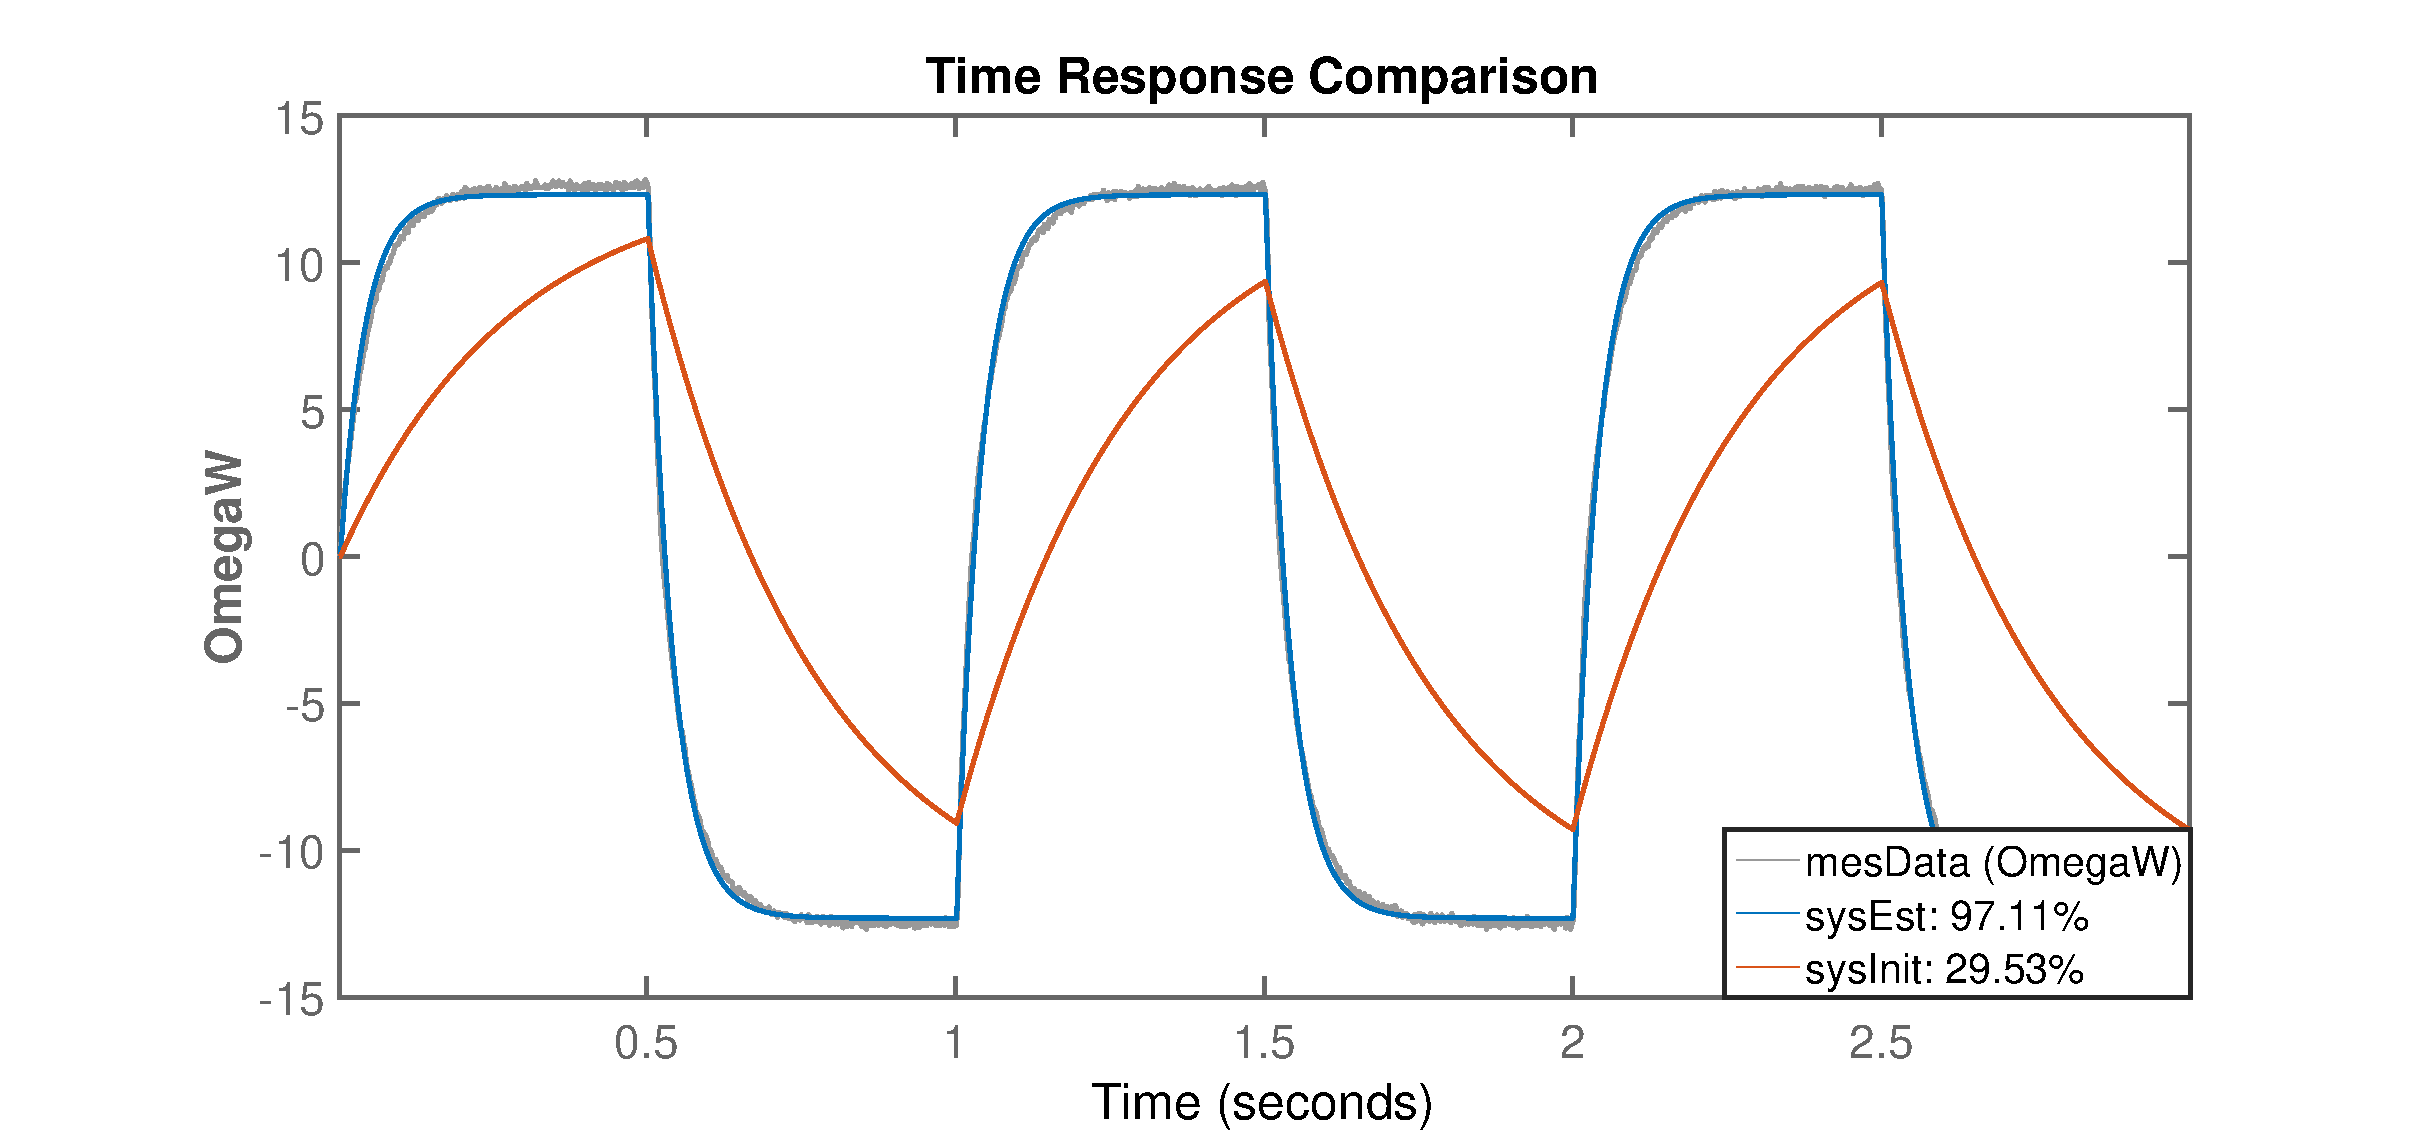
\includegraphics[width = \textwidth]{ParameterEstimation.eps}
    \caption{Bode plot of the transfer function for the segway.}
    \label{fig:paramEst1}
\end{figure} 

With the new gain, the response can be seen in \autoref{fig:paramEst1}, where the model prediction, shown in orange, is shown together with the measured data in grey. The blue axis is Matlab's estimate, based on the model type and measured data.

The model provided by matlab is tested on a different data set, where the motor voltage is changed from 1,96 V to -3,92 V. This can be seen in \autoref{fig:segwayBode_Merge}, where a correlation between the model and the data of $83 \% $ is obtained.

\begin{figure}[H]
    \centering
    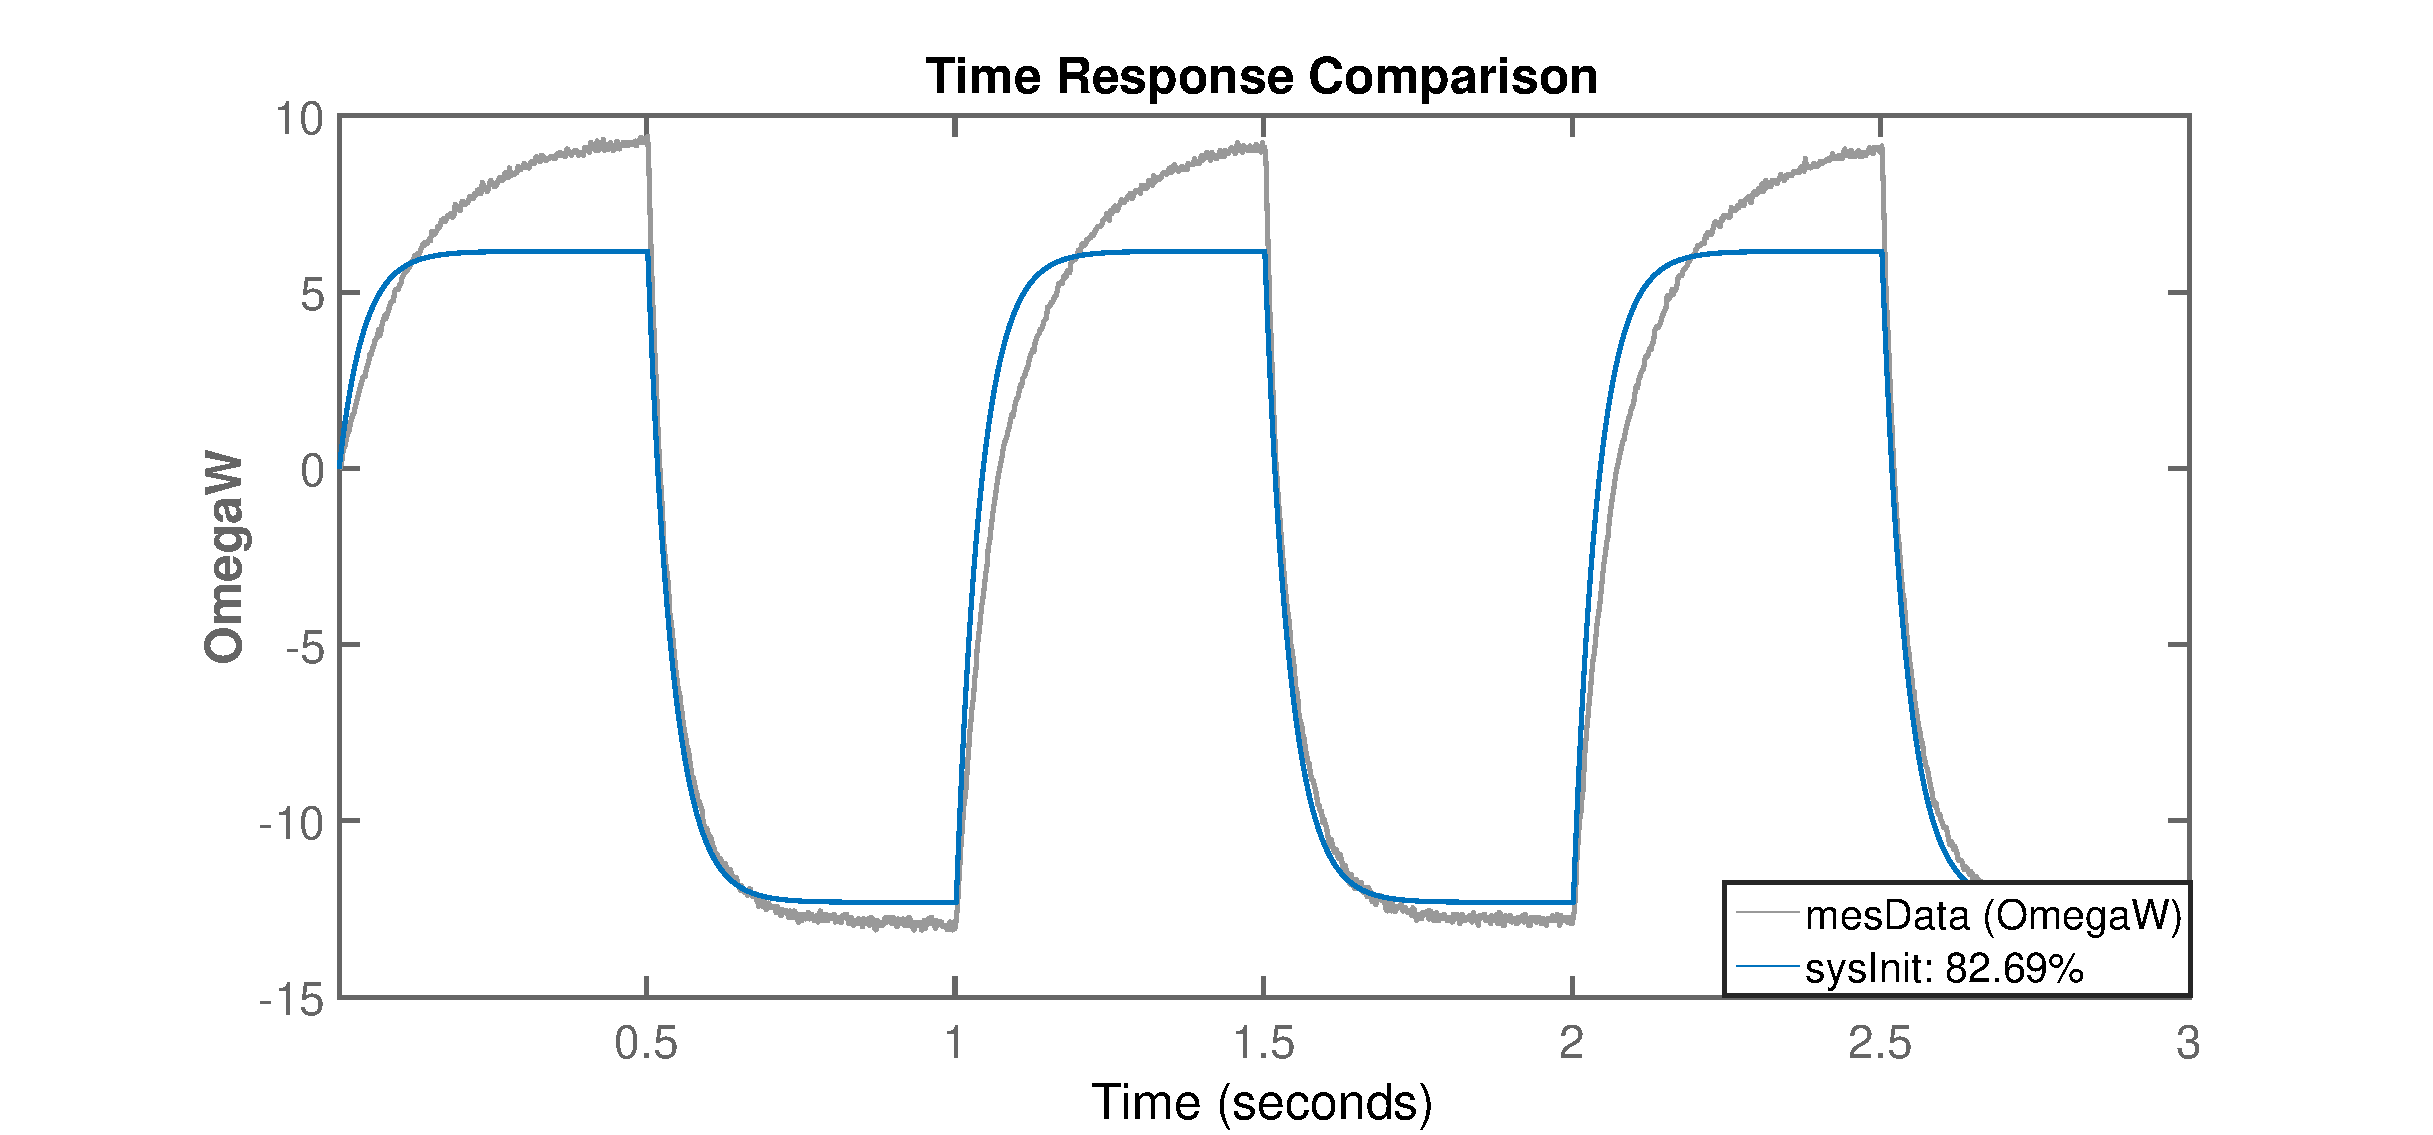
\includegraphics[width = \textwidth]{EstimationTest.eps}
    \caption{Bode plot of the transfer function for the segway.}
    \label{fig:paramEst2}
\end{figure} 

This is assumed to be satisfying, and thus the model for the motors and wheels has been found. Note that in the test, it is the transfer function $\frac{\omega_w{s}}{V_a(s)}$ that has been found, and thus the relationship between $\omega_w$ and $F_F$ as stated in \autoref{OmegaToForce} has to be taken into account. Doing this, results in the following transfer function:

\begin{equation}
\frac{F_F(s)}{V_a(s)} = \frac{0.049s}{0.040s + 1}
\label{eq:motorWheelFinal}
\end{equation}


\section{Model of Cart and Inverted Pendulum \label{sec:pen_model}}
In this section, a model of the inverted pendulum is derived. This model describes the movement of the cart and the inverted pendulum, based on governing equations put up regarding the behaviour of the system. To do this, it is necessary to investigate how the inverted pendulum moves, and how the interaction between the inverted pendulum and the cart can be described. Before this is done in detail, it is however first necessary to obtain an overview of the inverted pendulum.
\subsection{Overview of the Inverted Pendulum}
The model of the inverted pendulum describes how the two masses, i.e. the cart and the inverted pendulum, behaves when a force is exerted upon it by the surroundings. Note that the rod connecting the inverted pendulum mass to the cart is assumed massless, and is therefore not a part of the model. A schematic drawing of the inverted pendulum is shown in \autoref{fig:mecmodinvpen}.
\begin{figure}[H]
\centering
%\includegraphics[scale=1]{needstobechaged1.png}
\scalebox{0.6}{\input{figures/invpenmec.ralf}}
\caption{Mechanical model of the inverted pendulum.}
\label{fig:mecmodinvpen}
\end{figure}
In \autoref{fig:mecmodinvpen} the mass at the end of the rod is $m_p$, the variable $\theta_p(t)$ describes the angle of the inverted pendulum from a vertical line at the center of the cart. Note that the angle is positive in the counter-clockwise direction. This angle can be described in relation to both the x- and y-direction. The force applied to move the segway is labelled $F_F(t)$.\\\\
For simplicity, the coordinate system is defined such that $y_c(t)$ is 0, thus:
\begin{align}
x_p(t)&= x_c(t)- l \cdot \sin(\theta_p(t))\\
y_p(t)&= l\cdot \cos(\theta_p(t)) 
\end{align}
\begin{where}
\va{$x_p(t)$}{is the x-position of the inv. pendulum}{m}\\
\va{$x_c(t)$}{is the x-position of the cart}{m}\\
\va{$l$}{is the length between the center of rotation of the cart and the center of mass of the inv. pendulum}{m}\\
\va{$\theta_p(t)$}{is the angle of the inv. pendulum}{rad}\\
\va{$y_p(t)$}{is the y-position of the inv. pendulum}{m}\\
\end{where}

From this, the accelerations can be found by taking the double time differential of both sides of the above equations:
\begin{align}
\ddot x_p(t) &= \ddot x_c(t) + l \cdot \sin(\theta_p(t))\cdot \dot\theta_p^2 (t) - l \cdot \cos(\theta_p(t))\cdot \ddot\theta_p(t) \label{eq_acc_x}\\
\ddot y_p(t) &= -l\cdot \cos(\theta_p(t)) \cdot \dot\theta_p^2 (t) - l \cdot \sin(\theta_p(t))\cdot \ddot\theta_p (t)\label{eq_acc_y}
\end{align}
\begin{where}
\va{$\ddot x_p(t)$}{is inv. pendulum's acceleration in the x-direction }{rad/$\text{s}^2$}\\
\va{$\ddot \theta_p(t)$}{is inv. pendulum's angular acceleration}{rad/$\text{s}^2$}\\
\va{$\dot \theta_p(t)$}{is inv. pendulum's angular velocity}{rad/s}\\
\va{$\ddot y_p(t)$}{is inv. pendulum's acceleration in the y-direction }{rad/$\text{s}^2$}\\
\end{where}
%To make a transfer function for the inverted pendulum that can be merged with the transfer function for the motors and wheels, an equation in time domain describing the change in $\theta_p(t)$ caused by any $F_F(t)$ must first be derived. This is done in the following section.

To derive a model expression for the inverted pendulum, which shall be combined with a model expression for the motors and wheels, an equation %in time domain 
 describing the change in $\theta_p(t)$ caused by any $F_F(t)$ must first be derived. This is done in the following section.
\subsection{Equations of Motion}
In this section, translatoric free body diagrams for the cart and the inverted pendulum are presented and used to derive equations of motion. From these, a model of the cart and the inverted pendulum can be obtained.
 %\todo{is it still the only purpose, i think it has changed.A}The goal of this section is to arrive at one expression with only two variables, namely the input, $F_F(t)$ and the output, $\theta_p(t)$ of the model for the inverted pendulum. %Subsequently this expression is verified through simulation, and comparison with expected result.
\newpar
From \autoref{fig:mecmodinvpen}, free body diagrams can be determined. In this case, the cart's and the inverted pendulum's free body diagrams are representing the forces acting upon them while the segway is at an angle, $\theta_p(t)$.\\
The free body diagram of the mass at the end of the rod, is shown in \autoref{fig:fbdm1}.
\begin{figure}[H]
%\hspace{-0.5 cm}
\centering
\begin{subfigure}[b]{0.42\textwidth}
		\hspace{1.5cm}
        \scalebox{0.6}{\input{figures/invpen_M2_FBD.ralf}}
        %\vspace{3mm}
		\caption{FBD of the cart.}
		\label{fig:fbdm2}
\end{subfigure}
\hspace{1 cm}
\begin{subfigure}[b]{0.42\textwidth}
		\centering
        \scalebox{0.6}{\input{figures/invpen_M1_FBD.ralf}}
        %\vspace{10 mm}		
		\caption{FBD of the pendulum mass.}
		\label{fig:fbdm1}
    \end{subfigure}  
\caption{Free body diagrams of the mass of the inverted pendulum and the mass of the cart.}
\label{fig:FBDMotorWheel}
\end{figure}
\clearpage
The forces acting on the the mass $m_p$ is the gravitational force $F_g$, and the tension in the rod between the cart and the inverted pendulum, $F_t(\theta_p(t))$. This force is split up into two composants - a composant in the x-direction, $F_{tx}(\theta_p(t))$ and one in the y-direction, $F_{ty}(\theta_p(t))$. % The magnitude of this force depends on the angle, $\theta_p(t)$.\\
\autoref{fig:fbdm2} shows the free body diagram of the segway's cart. The force $F_g$ is the gravitational force and $F_N$ is the force pushing upwards from the ground. Note that the magnitude of the tension force $F_t(\theta_p(t))$ is equal to the force acting upon the inverted pendulum, but in opposite direction. %Furthermore, the force $F_F(t)$ from \autoref{fig:mecmodinvpen} has been split in two forces, namely $F_{F1}$ and $F_{F2}$, because there are two motors applying this force. The forces $F_{F1}$ and $F_{F2}$ have the same direction and magnitude, as it is assumed that the motors apply the same force to the system. \newpar
From the free body diagrams, it is now possible to express the dynamics of the inverted pendulum with the following three equations of motion. \\\\
For the inverted pendulum:
\begin{align}
m_p \cdot \ddot x_p(t) &= - F_{tx}(\theta_p(t)) \label{eom1}\\
m_p \cdot \ddot y_p(t) &= F_{ty}(\theta_p(t)) - F_g \label{eom2}
\end{align}
\begin{where}
\va{$m_p$}{is the mass of the inv. pendulum}{kg}\\
\va{$\ddot x_p(t)$}{is inv. pendulum's acceleration in the x-direction}{$\text{m}/\text{s}^2$}\\
\va{$F_{ty}(\theta_p(t))$}{is the rod's tension force in the y-direction}{N}\\
\va{$F_{tx}(\theta_p(t))$}{is the rod's tension force in the x-direction}{N}\\
\va{$\theta_p(t)$}{is inv. pendulum's angle from cart's center}{rad}\\
\va{$\ddot y_p(t)$}{is inv. pendulum's acceleration in the y-direction}{$\text{m}/\text{s}^2$}\\
\va{$F_g$}{is the gravitational force}{N}\\
\end{where} 

Note that \autoref{eom1} is for the horizontal direction and \autoref{eom2} is for the vertical direction. For the cart, it is only relevant to sum the forces in the horizontal direction, as it is assumed that the surface the cart moves on is immovable. 
\begin{align}
m_c \cdot \ddot x_c(t) = F_{tx}(\theta_p(t))+ F_{F}(t)\label{eom3}
\end{align}
\begin{where}
\va{$m_c$}{is the mass of the cart}{kg}\\
\va{$\ddot x_c(t)$}{is the cart's acceleration in the x-direction}{$\text{m}/\text{s}^2$}\\
\va{$F_{F}(t)$}{is the applied force from the motors}{N}\\
\end{where}

From equation \autoref{eom3} it can be deducted that the load force $F_L$ is equivalent to $F_{tx}$ since this is the contribution from the inverted pendulum. By combining \autoref{eq_acc_y}, \ref{eom1} and \ref{eom3} the governing equation for cart's movement can be obtained.
\begin{equation}
m_c \cdot \ddot x_c(t) = F_{F}(t) - m_p\left(\ddot x_c(t) + l \cdot \sin(\theta_p(t))\cdot \dot\theta_p^2(t) - l \cdot \cos(\theta_p(t))\cdot \ddot\theta_p(t)\right)\label{eq:model_pen33}
\end{equation}

From this, it can be seen that the load force can be described as:
\begin{equation}
F_L = m_p\left(\ddot x_c(t) + l \cdot \sin(\theta_p(t))\cdot \dot\theta_p^2(t) - l \cdot \cos(\theta_p(t))\cdot \ddot\theta_p(t)\right)
\label{loadForce}
\end{equation}
%Note that from this, the load torque to the motors can be found. 
%\autoref{eq:model_pen33} states that the resultant force acting on the cart is equal to the applied force, minus the contribution from the pendulum, which is the last term in \autoref{eq:model_pen33}. Thus, if the resultant force is to be the same as the applied, the motor is to overcome the contribution from the pendulum. In this respect, the last term in \autoref{eq:model_pen33} can be seen as the load torque to the motors, when multiplied with the wheel radius, i.e.:
%\begin{equation}
%\tau_L(t) = r_w \cdot m_p\left(\ddot x_c(t) + l \cdot \sin(\theta_p(t))\cdot \dot\theta_p^2(t) - l \cdot \cos(\theta_p(t))\cdot \ddot\theta_p(t)\right) 
%\label{tauLDef}
%\end{equation}

%The equations of motion for both the pendulum and the cart are all translatoric. To eliminate the variables $\ddot x_1(t)$ and $\ddot y_1(t)$ kinematics is applied. From the principles  of kinematics the equations of motion can be expressed in only rotational terms. The acceleration of the pendulum is a sum of the acceleration of the pendulum in relation to the cart and the acceleration of the cart.

Now, the translatoric movement of the inverted pendulum has been described, and the rotation thus needs to be described. The rotation of the inverted pendulum is described from the resultant torque acting on the inverted pendulum, denoted as $J_p \ddot{\theta_p}(t)$. The rotation of the inverted pendulum occurs around the center of mass of the inverted pendulum. From \autoref{torqueDeriviation}, it can be seen that there are three forces determining the rotation of the inverted pendulum, namely the gravitational force, $F_g$, and the x- and y-composants of the tension force, namely $F_{tx}$ and $F_{ty}$.

\begin{figure}[H]
\centering
\scalebox{0.6}{\input{figures/modellingSeg.ralf}}
%\input{figures/modellingSeg.ralf}
\caption{The forces contributing to the resultant torque of the inverted pendulum.}
\label{torqueDeriviation}
\end{figure}

The mentioned forces exert a torque on the inverted pendulum based on their distance from the center of rotation. In the case of the segway, the arm is the length of the rod, where the forces acting upon it are $F_{tx}$ and $F_{ty}$. It can be seen that $F_g$ attacks at the point mass, resulting in the arm length being zero and is therefore not acting upon the inverted pendulum. 
It should be noted that it is only the composant of the forces which are perpendicular to the rod that contributes to the torque, which needs to be included in the torque expressions. 
Thus, summing over the torques, the resultant pendulum torque can be described as:

\begin{equation}
J_p \ddot{\theta_p}(t) =  l \cdot \sin(\theta_p) F_{ty}-l \cdot \cos(\theta_p) F_{tx} \label{eq:gov2}
\end{equation}
\begin{where}
\va{$J_p$}{is the inertia of the inverted pendulum}{kg $m^2$}\\
\end{where}

A governing equation for the inverted pendulum can be obtained by inserting \autoref{eq_acc_x} in \autoref{eom1} and \autoref{eq_acc_y} in \autoref{eom2} and inserting these expressions in \autoref{eq:gov2}:
\begin{align}
\begin{split}
J_p \ddot{\theta_p}(t) &= m_p \cdot l \cdot \sin(\theta_p(t))\left(g -l \cdot \cos(\theta_p(t))\cdot \dot \theta_p^2(t) - l \cdot \sin(\theta_p(t)) \cdot \ddot \theta_p(t)\right)\\&+m_p \cdot l \cdot \cos(\theta_p(t))\left(\ddot x_c(t) - l \cdot \sin(\theta_p(t))\cdot \dot \theta_p^2(t) - l \cdot \cos(\theta_p(t)) \cdot \ddot \theta_p(t)\right)
\end{split}
\end{align}

Expanding this and using simple geometric relations, the expression can be simplified to:
\begin{equation}
(J_p+m_p\cdot l^2)\cdot \ddot \theta_p(t) = m_p \cdot l \cdot \left(\sin(\theta_p(t)) \cdot g+ \cos(\theta_p(t)) \cdot \ddot x_c(t)\right) \label{eq:inertia1}
\end{equation}

%The acceleration of the pendulum in relation to the cart can only be in a circle around the cart. The pendulums acceleration around the circle, is the sum of two accelerations. Namely the tangent acceleration in the direction described by $\vv{\epsilon_\theta}$ and the centripetal acceleration in the direction described by $\vv{\epsilon_r}$ and shown in \autoref{fig:invPenKin}
%Thus the acceleration of the pendulum can be expressed as \autoref{eom4}.
%
%\begin{figure}[H]
%\centering
%\scalebox{0.6}{\input{figures/invpenmec_kin.ralf}}
%\caption{Mechanical model of the inverted pendulum with the direction of the centripetal acceleration and the tangent acceleration.}
%\label{fig:invPenKin}
%\end{figure}
%
%\begin{align}
%\vv{a_p} = l\cdot \ddot \theta(t)\cdot \vv{\epsilon_\theta} + l \cdot \dot \theta(t) ^2 \cdot \vv{\epsilon_r} + \ddot x_c = \vv{a_{p/c}}+\vv{a_c} \label{eom4}
%\end{align}
%\begin{where}
%\va{$\vv{a_p} $}{is the vector describing the acceleration of the pendulum}{$\frac{\text{m}}{\text{s}^2}$}\\
%
%\va{$\vv{\epsilon_\theta}$}{is the vector describing the direction of the tangent acceleration}{1}\\
%\va{$\dot\theta(t)$}{is the angular velocity}{$\frac{\text{rad}}{\text{s}}$}\\
%\va{$\vv{\epsilon_r}$}{is the vector describing the direction of the centripetal acceleration}{1}\\
%\va{$\vv{a_{p/c}}$}{is the vector describing the acceleration of the pendulum relative to the cart}{$\frac{\text{m}}{\text{s}^2}$}\\
%\va{$\vv{a_c}$}{is the vector describing the acceleration of the cart}{$\frac{\text{m}}{\text{s}^2}$}
%\end{where}
%
%Expanding \autoref{eom4}'s vectors, so the accelerations are expressed in terms of the x- and y-directions, will give the following two equations.
%\begin{align}
%\ddot x_p(t)&=\vv{a_{px}}= -l \cdot \ddot\theta_p(t)\cdot \cos(\theta_p(t)) + l \cdot \dot \theta_p(t)^2 \cdot \sin(\theta_p(t))+\ddot x_c(t)  \label{eom5} \\
%\ddot y_p(t)&=\vv{a_{py}}=-l\cdot \ddot\theta_p(t)\cdot\sin(\theta_p(t)) - l \cdot \dot \theta_p(t)^2 \cos(\theta_p(t))-g\label{eom6}
%\end{align}
%
%\begin{where}
%\va{$\vv{a_{px}}$}{is the vector describing the pendulums acceleration in the x-direction}{$\frac{\text{m}}{\text{s}^2}$}\\
%\va{$\vv{a_{py}}$}{is the vector describing the pendulums acceleration in the y-direction}{$\frac{\text{m}}{\text{s}^2}$}
%\end{where}
%
%
%$\ddot x_p(t)$ and $\ddot y_p(t)$ is eliminated, by inserting \autoref{eom5} into \autoref{eom1} and \autoref{eom4} into \autoref{eom2}, yielding \autoref{eom7} and \autoref{eom8} respectively.
%
%\begin{align}
%-m_p\cdot l\cdot \ddot \theta_p(t) \cdot \cos(\theta_p(t))+m_p \cdot l\cdot \dot \theta_p^2(t) \cdot \sin(\theta_p(t))+m_p\cdot \ddot x_c(t)= - F_t(\theta_p(t)) \cdot \sin(\theta_p(t)) \label{eom7}
%\end{align}
%\begin{align}
%-m_p \cdot l \cdot \ddot \theta_p(t)\cdot\sin(\theta_p(t)) - m_p \cdot l\cdot \dot \theta_p^2(t) \cdot \cos(\theta_p(t))= F_t(\theta_p(t)) \cdot \cos(\theta_p(t)) - m_p \cdot g \label{eom8}
%\end{align}
%
%\begin{where}
%\va{$g$}{is the gravitational acceleration}{$\frac{\text{m}}{\text{s}^2}$}\\
%\end{where}
%
%\begin{figure}[H]
%\centering
%\includegraphics[width =0.3 \textwidth]{figures/inertia11.jpg}
%\caption{Tension force composants.}
%\label{fig:NewFig}
%\end{figure}
%
%From \autoref{fig:NewFig}, it can be seen that the tension force $F_t(\theta_p(t))$ can be slit into two composants, i.e. two forces perpendicular to each other. These can be described as:
%\begin{align}
%F_{t, x}(\theta_p(t)) &= - F_t(\theta_p(t)) \cdot \sin(\theta_p(t))\\
%F_{t, y}(\theta_p(t)) &= F_t(\theta_p(t)) \cdot \cos(\theta_p(t))
%\end{align}
%
%These forces can be used to obtain an expression for the resultant torque acting on the pendulum. From \todo{source: matlab} it can be seen that the following relation applies:
%
%\begin{equation}
%J_p \ddot \theta_p(t) = - F_{t, x}(\theta_p(t)) \cdot l \cdot \cos(\theta_p) - F_{t, y}(\theta_p(t)) \cdot l \cdot \sin(\theta_p)
%\label{inertiaLink}
%\end{equation}
%
%By multiplying \autoref{eom7} with $\cos(\theta_p(t))$ and \autoref{eom8} with $\sin(\theta_p(t))$ then adding the two equations, the expression for the inertia as described in \autoref{inertiaLink} can be utilized, yielding \autoref{eom9}.
%
%Multiply with $l \cdot \cos(\theta)$ on both sides in \autoref{eom7}:
%\begin{align}
%-m_p\cdot l^2 \cdot \ddot \theta_p(t) \cdot \cos^2 (\theta_p(t))+m_p\cdot l^2 \cdot \dot \theta_p^2(t) \cdot \sin(\theta_p(t))\cdot \cos(\theta_p(t))+m_p\cdot l \cdot \ddot x_c \cdot \cos(\theta_p(t)) = F_{t, x}(\theta_p(t)) \cdot l \cdot \sin(\theta_p(t))\label{eom9}
%\end{align}
%
%Multiplying with $l \cdot \sin(\theta)$ on both sides in \autoref{eom8}:
%\begin{align}
%-m_p\cdot l^2 \cdot \ddot \theta_p(t)\cdot \sin^2 (\theta_p(t)) - m_p\cdot l^2 \cdot \dot \theta^2(t) \cdot \cos(\theta_p(t))\cdot \sin(\theta_p(t))=-m_p \cdot l \cdot g\cdot \sin(\theta_p(t)) - F_{t, y}(\theta_p(t)) \cdot l\cdot \sin(\theta_p(t)) \label{eom10}
%\end{align}
%
%Adding \autoref{eom9} and \autoref{eom10} and using the expression for the :
%
%
%
%To eliminate $\ddot x_c(t)$, an equation containing only the variables $\ddot x_c(t)$, $F_F$ and $\theta_p(t)$ and its derivatives must be constructed. This is done by substituting the left side of \autoref{eom7} into \autoref{eom3} in place of $F_t(\theta_p(t)) \cdot sin(\theta_p(t))$. This yields \autoref{eom10}.
%\begin{align}
%(m_p+m_c)\cdot \ddot x_c(t)=m_p\cdot l\cdot \ddot \theta_p(t) \cdot \cos(\theta_p(t))-m_p\cdot l\cdot \dot \theta_p(t)^2 \cdot \sin(\theta_p(t))+F_F(t)\label{eom10}
%\end{align}
%
%With 2 equations containing $\ddot x_c(t)$, this variable is now eliminated by isolating $\ddot x_c(t)$ in \autoref{eom9} and inserting this expression for $\ddot x_c(t)$ in \autoref{eom10}. This yields \autoref{eq:thetaForce}.
%\begin{align}
%\ddot \theta_p(t)(l\cdot (m_p + m_c)-m_p \cdot l \cdot \cos^2(\theta_p(t)))&+\dot\theta_p(t)^2 \cdot (m_p\cdot l\cdot \sin(\theta_p(t))\cdot \cos(\theta_p(t)))\nonumber\\ 
%&=  \\
%\cos(\theta_p(t))\cdot F_F(t)+g\cdot &\sin(\theta_p(t))\cdot (m_p+m_c)\nonumber\label{eq:thetaForce}
%\end{align}
%
%\autoref{eq:thetaForce} contains only two variables, namely $\theta_p(t)$ and $F_F(t)$, thus this single expression describes the motion of the inverted pendulum. This model is clearly not linear, thus it has to be linearised before a transfer function can be determined. This is done in the next subsection.
%
%%In the following section, a block diagram is build from this expression, through which the expression is verified by simulation and subsequent comparison with expected result.
%%changed due to mistak where L was not included.
%%\begin{align}
%%\ddot \theta (-m_1\cdot L \cdot \cos^2(\theta)+(m_1+m_2)\cdot L)+\dot \theta^2(m_1\cdot \sin(\theta)\cdot \cos(\theta))=F_F+(m_1+m_2)\cdot g\cdot \sin(\theta)
%%\end{align}
%The model of the inverted pendulum without the inertia can be expressed as: 
%\begin{equation}
%(m_p+m_c)\cdot \ddot x_c(t)= m_p\cdot l \cdot \ddot \theta_p(t) \cdot \cos(\theta_p(t))-m_p \cdot l \cdot \dot \theta_p(t)^2 \sin(\theta_p(t))+2\cdot F_F(\theta_p(t))\label{eq:penmodelnoinertia}
%\end{equation}
%
%Note, that $F_F(\theta_p(t))$ is multiplied by two, as there are two wheels applying force. \\
%This expression can be combined with \autoref{eq:inertia1}. 
%This is done by isolating $\ddot x_c(t)$ in \autoref{eq:penmodelnoinertia}. Inserting this into \autoref{eq:inertia1} yieds: 
%\begin{align}
%&(J_p+m_p\cdot l^2)\cdot (m_p + m_c)\cdot \ddot \theta_p(t)=(m_p^2 +m_p\cdot m_c)\cdot l \cdot g \cdot \sin(\theta_p(t))\nonumber \\&+m_p^2\cdot l^2\cdot \cos^2(\theta_p(t)) \cdot \ddot \theta_p(t)-m_p\cdot l \cdot \dot \theta_p(t)^2\cdot \sin(\theta_p(t))+2\cdot F_F(\theta_p(t))\label{eq:final_pen22}
%\end{align}
\autoref{eq:model_pen33} and \autoref{eq:inertia1} are the final model expressions for the inverted pendulum. The next step before transfer functions are derived, is to linearize these expressions. This is done in the following section.
\vspace{1 cm}
%This can now be combined with the model expression of the motors and wheels model. This is done in the following section. 
% This will be linearized in the following section and combined with the already linear motormodel. This will lead to a transferfunction for the system, which is to be simulated. From this a controller can be designed and later implemented. 
%\input{design/modelling/Inv_pen_model_non_lin.tex}
\section{Derivation of Segway Transfer Functions}
In this section, the model expressions derived in previous sections are verified, linearized and combined into transfer functions. From these transfer functions, the controllers will be designed to allow the segway to balance in an upright position. In this section, the models are viewed and linked as illustrated in \autoref{fig:modelOverallLin}.
\begin{figure}[H]
\centering
\begin{tikzpicture}[auto, node distance=3.5cm,>=latex']
    % We start by placing the blocks
    \node [input, name=input] {};

    % Once the nodes are placed, connecting them is easy. 
	\draw[thick,dashed, fill=black!10, align=center] ($(input.north west)+(15.5,-1)$) rectangle ($(input.north west)+(0.6,2.75)$);
	\draw[thick,dashed, fill=black!30, align=center] ($(input.north west)+(10.75,-0.8)$) rectangle ($(input.north west)+(1.5,1.75)$);
	 \node [align=center] at ($(input.north west)+(8,2.25)$) {\textbf{Plant, }$\mathbf{ \, \, \, G}$};
	 \node [align=center] at ($(input.north west)+(6,1.25)$) {{Motors and Wheels Model}};
	
	\node [blockbig, right of=input, align = center] (motor) {Motor \\ and Wheel};
	\node [blockbig, right of=motor, align = center, node distance=4.5cm] (Cart) {Cart \\ Movement};
    \node [blockbig, right of=Cart, align = center, node distance=4.5cm] (pendulum) {Inverted \\ Pendulum};

   \node [output, right of=pendulum, node distance=3.5cm] (output) {};

	
    \draw [->] (input) -- node {$V_a$} (motor);
    \draw [->] (4.75,0.2) -- node {$\tau_a$} (6.75,0.2);
    \draw [->] (9.25,0.2) -- node {$\theta_w$} (11.25,0.2);
    \draw [->] (11.25,-0.2) -- node {$F_L$} (9.25,-0.2);
   % \draw [->] (9.75,-0.2) -| node {} (3.75,-0.2);
    \draw [->] (pendulum) -- node {$\theta_p$} (output);
\end{tikzpicture}
\caption{Block diagram of the plant, also known as system model.}
\label{fig:modelOverallLin}
\end{figure}
Note that the models are linked differently than previously shown in \autoref{fig:modelOverall}, since the cart movement is made part of the motor and wheel model, instead of being part of the inverted pendulum model. This is because it is not possible to measure the torque $\tau_a$, while the wheel angle, $\theta_w$, can be measured by the encoders. Thus, it will be possible to derive a transfer function for the motors and wheels model. The same applies for the inverted pendulum model, where it will be possible to derive and verify a transfer function based on an input being the wheel angle, $\theta_w$, instead of the torque $\tau_a$.
\subsection{Verification of Models}
The three model expressions that have been derived in the previous sections are \autoref{eq:MotorFinal}, \ref{eq:model_pen33} and \ref{eq:inertia1}. For repetition, these are shown below.
\begin{align}
\tau_a(t) = \frac{1}{N_{ms} N_{sw}}\Big(\frac{k_t}{R_a} \big( V_a(t)& - k_e \dot\theta_m(t) \big) - \ddot\theta_m(t)J_{T} - \dot\theta_m(t)B_{T}\Big)
\label{eq:model3}\\
m_c \cdot \ddot x_c(t) = F_F(V_a(t)) - m_p\Big(\ddot x_c(t)& + l \cdot \sin(\theta_p(t))\cdot \dot\theta_p^2(t) - l \cdot \cos(\theta_p(t))\cdot \ddot\theta_p(t)\Big)\label{eq:model2}\\
(J_p+m_p\cdot l^2)\cdot \ddot \theta_p(t) = m_p \cdot l \cdot &\left( \sin(\theta_p(t)) \cdot g+\cdot \cos(\theta_p(t)) \cdot \ddot x_c(t) \right) \label{eq:model1}
\end{align}

If no slip is assumed in the gearing and between the wheels and the ground, then $\dot \theta_m(t)$ and $\ddot \theta_m(t)$ can be replaced with $N_{ms}N_{sw} \cdot \dot \theta_w(t)$ and $N_{ms}N_{sw} \cdot \ddot \theta_w(t)$ respectively, and $\ddot x_c(t)$ can be replaced with $r_w \cdot \ddot \theta_w(t)$. This yields the three governing equations for the system model:
\begin{align}
\tau_a(t) =\frac{\left( \frac{K_t}{R_a} \left( V_a(t) - \frac{K_e }{N_{ms} N_{sw}} \cdot \dot\theta_w(t) \right) - \frac{J_{T}}{N_{ms} N_{sw}} \cdot \ddot\theta_w(t) - \frac{B_{T}}{N_{ms} N_{sw}} \cdot \dot\theta_w(t) \right)}{N_{ms} N_{sw}}
\label{eq:model3W}\\
m_c \cdot r_w \cdot \ddot \theta_w(t) = F_F(V_a(t)) - m_p\left(\ddot \theta_w(t) \cdot r_w + l \cdot \sin(\theta_p(t))\cdot \dot\theta_p^2(t) - l \cdot \cos(\theta_p(t))\cdot \ddot\theta_p(t)\right)\label{eq:model2W}\\
(J_p+m_p\cdot l^2)\cdot \ddot \theta_p(t) = m_p \cdot l \cdot \left( \sin(\theta_p(t)) \cdot g+\cdot \cos(\theta_p(t)) \cdot r_w \cdot \ddot \theta_w(t) \right) \label{eq:model1W}
\end{align}

To form the governing equation for the motors and wheels model, \autoref{eq:model3W} and \autoref{eq:model2W} are to be combined, see \autoref{fig:modelOverallLin}. 
To meet the interfaces specified, see \autoref{fig:modelOverallLin}, the relation between the motor and wheel model's output $\tau_a(t)$ and the force $F_F(t)$ which the cart movement model has as input, see \autoref{eq:model3W}, must be determined. 

There are two motors in the system, each exerting a torque, $\tau_a(t)$, which has to be included. A torque can be expressed as a force acting at a certain distance from the rotation point, also known as an arm. In this case, the arm is the wheel radius, so by using this, the force acting on the cart can be found. This relation can be expressed as:
%  some  that this transfer function has the input $V_a$ and the output $\theta_w$. To achieve this, The relation is seen in \autoref{eq:tauFFrelation}.
\begin{equation}
F_F(t) = 2\cdot \tau_a(t) \cdot \frac{1}{r_w}\label{eq:tauFFrelation}
\end{equation}
Inserting the motor and wheel model, \autoref{eq:model3W}, into \autoref{eq:tauFFrelation} yields:
\begin{equation}
F_F(t) = 2\cdot \frac{\Big(\frac{K_t}{R_a} \left( V_a(t) - \frac{K_e}{N_{ms} N_{sw}} \cdot \dot\theta_w(t) \right) - \frac{J_{T}}{N_{ms} N_{sw}} \cdot \ddot\theta_w(t) - \frac{B_{T}}{N_{ms} N_{sw}} \cdot \dot\theta_w(t) \Big)}{r_w \cdot N_{ms} N_{sw}}\label{eq:motorFF}
\end{equation}
Combining \autoref{eq:motorFF} and \autoref{eq:model2W} and using the fact that $\dot \theta_m(t) = \omega_m(t)$ yields:
\begin{align}
\begin{split}
m_c \cdot r_w \cdot \dot \omega_w(t) = \, &2 \cdot \frac{\Big(\frac{K_t}{R_a} \left( V_a(t) -  \frac{K_e}{N_{ms} N_{sw}} \cdot \omega(t) \right) - \frac{J_{T}}{N_{ms} N_{sw}} \cdot \dot\omega_w(t) - \frac{B_{T}}{N_{ms} N_{sw}} \cdot \omega_w(t) \Big)}{r_w \cdot N_{ms} N_{sw}} \\ \\
 &- m_p\left(r_w \cdot \dot \omega_w(t) + l \cdot \sin(\theta_p(t))\cdot \dot\theta_p^2(t) - l \cdot \cos(\theta_p(t))\cdot \ddot\theta_p(t)\right)
\end{split}\label{motorsAndWheels}
\end{align}
This differential equation describes the movement of the motors and wheels, and is simulated using Simulink, by inserting the values in the expression as found in \appref{app:segwayParameters} and \appref{motorMeasReport} and applying a voltage step to the model. Since it is desired to test the relationship between the voltage applied to the motors and the movement of the cart, the final term in \autoref{motorsAndWheels} is set to zero. This is because this term is equal to $F_L$, as can be seen in \autoref{loadForce}, i.e. this term describes the inverted pendulum's influence on the movement of the cart, which is disregarded in this test. The result of the test can be seen in \autoref{fig:motor1}. 
\begin{figure}[H]
\centering
\includegraphics[height = 0.75\textwidth, angle = -90]{figures/motor1.pdf}
\caption{Simulation of motors and wheels model with an applied step as input.}
\label{fig:motor1}
\end{figure}
Looking at the expression for the motors and wheels model in \autoref{motorsAndWheels}, it is seen that the system is a first order when removing the final term in the expression. This is because the highest order of derivatives of $\omega_m(t)$ is one, giving a first order transfer function. This is partly due to the approximation done in \autoref{eq:electricMotor2} about disregarding the inductance in the motor.
From \autoref{fig:motor1}, it can be seen that the output of the motor mimics a first order system's output, as the response is approaching the reference, without any oscillation or overshoot, which is not possible for a first order system. Therefore, the output of the simulation matches what is expected, and the model is therefore assumed to be valid.

The inverted pendulum model \autoref{eq:model1W} is also simulated in Simulink. The input to this model is chosen to be $\ddot{x}_c$ since this is the input parameter in \autoref{eq:model1W}, by means of the expression $\ddot{x}_c = r_w\ddot{\theta}_w$. Also note that the inverted pendulum is initialised at an angle of -0.05 rad. The result can be seen in \autoref{fig:pend1}.
\begin{figure}[H]
\centering
\includegraphics[height = 0.75\textwidth, angle = -90]{figures/pend1.pdf}
\caption{Simulation of the inverted pendulum model with an applied step as input.}
\label{fig:pend1}
\end{figure}

From \autoref{fig:pend1} it can be seen that the inverted pendulum starts tilting to one side, and when the step is applied, the angle changes direction and lastly the inverted pendulum oscillates around a certain angle. This angle is $\pi$ if the pendulum is swinging freely, corresponding to it hanging downwards, however an offset from $\pi$ is seen, due to the step applied. Thus, the inverted pendulum model is assumed to be valid.

To validate the system model, the motors and wheels model and the inverted pendulum model are combine and simulated in MATLAB. As an initial conditions for the simulation, the inverted pendulum is set at an angle of 1 radian, as this will cause the inverted pendulum to fall. Furthermore, a small friction is inserted in the inverted pendulum model to make the result comply more with expectations. This is done because the angle's magnitude otherwise grows, i.e. the inverted pendulum will oscillate more violently over time. This can be due to a sign error on a small number in the model. Time constraints prohibits the localisation and correction of this minor issue. The results of the simulation can be seen in \autoref{fig:systemVerification}.

\begin{figure}[H]
\centering
\includegraphics[height = 0.85\textwidth, angle = -90]{systemVerification.pdf}
\caption{Simulation of the system model by setting the inverted pendulum at 1 radian and no input. Note: a small friction is inserted in the model to comply more with expectations.}
\label{fig:systemVerification}
\end{figure}

From \autoref{fig:systemVerification}, it can be seen that the pendulum slowly loses magnitude due to the inserted friction. Also, it oscillates around $\pi$ which is to be expected. The model is hereby validated and can now be linearised.


\subsection{Linearisation of Derived Equations of Motion\label{subsec:Linearization}}
%In this section a transfer function describing the system is derived. This is done based on the three model equations, describing the behaviour of the segway. The transfer function is derived, so that it can be used when designing the controller. 
Before a transfer function of the system can be derived, it is necessary to linearise the two model equations, \autoref{eq:model1W} and \ref{motorsAndWheels}, as it is only linear equations that can be Laplace-transformed to form a transfer function.

It is seen that the only part of the motors and wheels model, \autoref{motorsAndWheels}, that is non-linear comes from \autoref{eq:model2W}, thus only this part needs to be linearised.
The second model equation, \autoref{eq:model1W}, also needs to be linearised as it contains non-linear terms. 

The method for doing the linearisation is chosen to be Taylor expansion.
%The last term in \autoref{motorsAndWheels} is the load torque $\tau_L$ \todo{why?}, and is approximately zero near the segway's operating point \todo{why?}. Thus \autoref{eq:motorsAndWheels} can be approximated as:
%\begin{equation}
%m_c \cdot r_w \cdot \ddot \theta_w(t) = 2 \cdot \frac{\Big(\frac{K_t}{R_A} \left( V_a(t) - K_e \cdot \frac{1}{N_{ms} N_{sw}} \cdot \dot\theta_w(t) \right) - \frac{1}{N_{ms} N_{sw}} \cdot \ddot\theta_w(t)J_{T} - \frac{1}{N_{ms} N_{sw}} \cdot \dot\theta_w(t) \cdot B_{T}\Big)}{r_w \cdot N_{ms} N_{sw}} \label{eq:model2S}
%\end{equation} 
%This approximation does not only simplify the expression considerably, but it also makes it a linear equation, as the load torque is the only nonlinear term in \autoref{eq:motorsAndWheels}.
%When approximating the load torque, it should be noted that it is only valid when the segway is at its operating point or very close to it. As the linearisation of the last model expression, \autoref{eq:model1W}, will be in the operating point as well, does not reduce the validity of the linearised model.\\
When linearising an equation, an expression for the tangent to the operating point is derived. 
% however is not alarming as the linearization of the other models, will be done in the equillibrium point as well.
%will be an approximation based on an operating point, which is in the segways equillibium position.\newpar
%The linearised model is the tangent to the chosen operating point. 
This is shown in \autoref{fig:taylor}. %This approach means that the linearised model is only an approximation of the original model around the operating point.
%During the course Modelling and control, the group was introduced to Taylor expansion as a method to linearise. For this reason the method that will be used to linearise \autoref{eq:model1W} is Taylor expansion.
\begin{figure}[H]
\centering
\input{figures/taylorFigure.ralf}
\caption{Illustration of linearisation principle.}
\label{fig:taylor}
\end{figure}

Taylor expansion is based on the Taylor series, shown in \autoref{eq:taylorSeries} \citep{sou:taylorSeries}. The Taylor series approximation of a signal is enhanced by including a greater number of terms in the Taylor series, i.e. by having an infinite sum of terms, the approximation is exact. However, since the linearisation is a tangent, only the first two terms in the Taylor series is used in the Taylor expansion, as the resulting expression is otherwise not linear.
\begin{align}
T(x) = f(a) + f'(a)(x - a) + \frac{f''(a)}{2!}(x - a)^2 + \frac{f^{(3)}(a)}{3!}(x - a)^3 + ...
\label{eq:taylorSeries}
\end{align}
\begin{where}
\begin{tabular}{p{40pt} p{42pt} p{200pt}} &$T$ & is the taylor approximation \end{tabular} \\
\begin{tabular}{p{40pt} p{42pt} p{200pt}} &$x$ & is the input \end{tabular} \\
\begin{tabular}{p{40pt} p{42pt} p{200pt}} &$f$ & is the function to be linearised \end{tabular} \\
\begin{tabular}{p{40pt} p{42pt} p{200pt}} &$a$ & is the linearisation point \end{tabular} \\
\end{where}

The linearisation is performed around the segway's operating point, which is expressed as:
\begin{equation}
\theta_p(t) = \bar{\theta}_p(t) + \hat{\theta}_p(t)
\end{equation}
\begin{where}
\va{$\theta_p(t)$}{is the angle of the inverted pendulum}{rad}\\
\va{$\bar{\theta}_p(t)$}{is the operating point}{rad}\\
\va{$\hat{\theta}_p(t)$}{is the deviation from the operating point}{rad}
\end{where}

There are three variables included in the non-linear terms in the equations that are to be linearised, i.e. $\theta_p(t)$, $\dot\theta_p(t)$ and $\ddot\theta_p(t)$. Therefore, the Taylor series has to be done for each variable, which can then be added to form the linear expression with multiple linearised variables. The Taylor expansion can be expressed as the following:
\begin{align}
T= f(\bar{\theta}_p(t),\bar{\dot \theta}_p(t), \bar{\ddot \theta}_p(t))+ \frac{\partial f(\bar{\theta}_p(t))}{\partial\theta_p(t)}\cdot \hat{\theta}_p(t)+\frac{\partial f(\bar{\dot \theta}_p(t))}{\partial \dot \theta(t)_p}\cdot \hat{\dot \theta}_p(t) &+ \frac{\partial f(\bar{\ddot \theta}_p(t))}{\partial \ddot \theta(t)_p}\cdot \hat{\ddot \theta}_p(t)\label{eq:taylor}
\end{align}

The linearisation is done in the segway's upright position $\theta_p = 0$, i.e. this is the chosen operating point.

First, the cart model, \autoref{eq:model2W}, is linearised. This is done in \appref{appTaylor}, and the result can be seen in \autoref{linGovEq2}.
\begin{equation}
(m_c + m_p) \cdot \ddot x_c(t) = F_{F}(t) + m_p \cdot l \cdot \hat{\ddot{\theta}}_p(t)\label{linGovEq2}
\end{equation}

Analysing this equation, and comparing it to \autoref{fig:systemVerification}, it is assumed that when the segway is being operated, i.e. a voltage is applied to the motors and the segway is therefore moving, the following is true:
$$ F_F(t) >> m_p \cdot l \cdot \hat{\ddot{\theta}}_p(t) $$
This means that the force applied from the motors is much bigger than the force the inverted pendulum exerts on the cart. Based on this assumption, the inverted pendulum's influence on the cart's position is neglected, i.e. the last term in \autoref{linGovEq2} is removed. In a physical sense, this would mean that when the inverted pendulum is tilting, the cart will not move. Obviously, this is not the case, but the movement caused by the inverted pendulum is much smaller than the movement caused by the motors and wheels, and it is therefore seen as a fair assumption to make. This serves to make the model simpler, by removing the feedback from the pendulum to the cart.\\
This simplified linearised expression can then be combined with \autoref{eq:model3W} and \autoref{eq:tauFFrelation}, to obtain a linear expression for the motors and wheels model, which can be seen in \autoref{eq:model2S}.
\begin{equation}
(m_c + m_p) \cdot r_w \cdot \ddot \theta_w(t) = 2 \cdot \frac{\Big(\frac{K_t}{R_a} \left( V_a(t) - \frac{K_e}{N_{ms} N_{sw}} \cdot \dot\theta_w(t) \right) - \frac{J_{T}}{N_{ms} N_{sw}} \cdot \ddot\theta_w(t) - \frac{B_{T}}{N_{ms} N_{sw}} \cdot \dot\theta_w(t) \Big)}{r_w \cdot N_{ms} N_{sw}} \label{eq:model2S}
\end{equation} 

With the motors and wheels model linearised, the inverted pendulum model shall also be linearised. The inverted pendulum model, see \autoref{eq:model1W}, is linearised in \appref{appTaylor}, which yields:
\begin{align}
(J_p+m_p\cdot l^2)\cdot \hat{\ddot \theta}_p(t) = m_p \cdot l \Big(g \cdot \hat{\theta}_p(t) + r_w \cdot \ddot \theta_w(t)   
\Big)\label{eq:firstModelLin}
\end{align}
Both model expressions are now linear and can be Laplace transformed to yield transfer functions, which is necessary to be able to design a controller for the segway. The segway's transfer function is now to be determined.
%The equation are shown in \autoref{eq:firstModel}, where each term that will be linearised by applying the Taylor expansion, shown in \autoref{eq:taylor}, is marked. The linearised approximation is shown in \autoref{eq:firstModelLin}.



%\subsection{Laplace Transform}
From the previous sections tree expressions have been derived. One for the motor model and one for the pendulum model. Moreover an expression, which is the link between the two models, is found. 
The motor model is the following:
\begin{equation}
\tau_a(t) = \frac{k_t}{R_A} \left( V_a(t) - K_e \cdot \dot\theta_m(t) \right) - \ddot\theta_m(t)J_{T} - \dot\theta_m(t)B_{T}  \label{eq:motorfinal2}
\end{equation}
Laplace transforming \autoref{eq:motorfinal2} yields:
\begin{align}
\tau_a(s)&=\frac{k_t}{R_A}- \Theta_m(s) (s\cdot \frac{k_t+k_e}{R_a}+s\cdot B_T+s^2\cdot J_T)\\
&=\frac{k_t}{R_A}- \Theta_m(s)(s^2\cdot J_T+s(\frac{k_t+k_e}{R_a}+B_T))
\end{align}
The link between the two models shall be laplace transformed as well. The link in time domain is:
\begin{align}
 \hat{\ddot\theta}_m(t)=\frac{(J_p+m_p\cdot l^2)\hat{\ddot \theta}_p(t)}{m_p\cdot l\cdot r_w\cdot N_{ms}\cdot N_{sw}}-\frac{g\cdot \hat{\theta}_p(t)}{r_w\cdot N_{ms}\cdot N_{sw}}\label{eq:linktime}
\end{align}
Laplace transforming \autoref{eq:linktime} yields:
\begin{align}
s^2\cdot \Theta_m(s)&= \frac{(J_p+m_p\cdot l^2)s^2\cdot \Theta_p(s)}{m_p\cdot l \cdot r_w \cdot N_{ms}\cdot N_{sw}}-\frac{g\cdot \Theta_p(s)}{r_w\cdot N_{ms}\cdot N_{sw}}\\
\Rightarrow \Theta_m(s)&= \frac{(J_p+m_p\cdot l^2)\Theta_p(s)}{m_p\cdot l \cdot r_w \cdot N_{ms}\cdot N_{sw}}-\frac{g\cdot \Theta_p(s)}{s^2 \cdot r_w\cdot N_{ms}\cdot N_{sw}}
\end{align}
Lastly the model for the pendulum. The model expression is: 
\begin{equation}
(J_p+m_p\cdot l^2)\hat{\ddot \theta}_p(t)(m_p+m_c)=(m_p^2+m_c)l\cdot g \cdot \hat{\theta}_p(t)+m_p^2\cdot l^2 \cdot  \hat{\ddot\theta}_p(t)+2\cdot F_F(\theta_p(t))\label{eq:penmodel11}
\end{equation}
Laplace transforming \autoref{eq:penmodel11} yields:
\begin{equation}
s^2(J_p+m_p\cdot l^2)\Theta_p(s)(m_p+m_c)=(m_p^2+m_c)l\cdot g \cdot \Theta_p(s) + m_p^2 \cdot l^2 \cdot s^2\cdot \Theta_p(s) +2\cdot F_F(\Theta_p(s))
\end{equation}
As the input to pendulum from the motors are the applied force, it is preferable to have this linearized model as an expression of the applied force. 
\begin{equation}
2\cdot F_F(\Theta_p(s))=\Theta_p(s)(s^2((J_p+m_p\cdot l^2)(m_p+m_c)-m_p^2\cdot l^2)-(m_p^2 + m_c)l\cdot g)
\end{equation}

%
%\begin{align}
%&s^2\cdot \theta\cdot (l\cdot (m_p+m_c-m_p))-\theta \cdot g(m_p+m_c)=F_F\nonumber\\
%&\Rightarrow \frac{\theta}{F_F}=\frac{1}{s^2\cdot (l\cdot (m_p+m_c)-g(m_p+m_c)}\nonumber \\
%&\Rightarrow \frac{\frac{1}{l\cdot m_c}}{s^2-\frac{g(m_p+m_c}{l\cdot m_c}}
%\end{align}
%It shows, that the transfer function is the same as the one derived at with the taylor expansion approximation. \\
%The linear approximation of the inverted pendulum model is therefore assumed valid. 
%
%
%
%%\Rightarrow\frac{2.377}{s^2 - 37.369}
%%\Rightarrow \theta(s)\cdot s^2\cdot l ((m_p+m_c)-m_p)=g\cdot \theta(s)\cdot (m_p+m_c)+F_F(s)\nonumber\\
%%\Rightarrow \theta(s)\cdot s^2\cdot l(m_p+m_c-m_p)-g\cdot \theta(s)\cdot(m_p+m_c)=F_F(t)\nonumber\\
%%\Rightarrow \theta(s)\cdot (s^2\cdot l \cdot (m_p+m_c))=F_F(t) \nonumber \\
%The transfer function for the inverted pendulum shall be merged with a transfer function for the motors and wheels model to allow design and implementation of a controller. Merging the transfer functions is done in the following section. 

%\section{Merging of models}
From the previous section three linearized expressions can be extracted. These are ow to be combinded such that a final expression is derived, representing the entire system.
The expressions are as follows:

\begin{align}
\tau_a(s)&=\frac{K_t}{R_A}- \Theta_m(s)\cdot(s^2\cdot J_T+s(\frac{k_t+k_e}{R_a}+B_T))\label{eq:1}\\
\Theta_m(s)&= \frac{(J_p+m_p\cdot l^2)s^2\cdot \Theta_p(s)}{m_p\cdot l \cdot r_w \cdot N_{ms}\cdot N_{sw}}-\frac{g\cdot \Theta_p(s)}{s^2 \cdot r_w\cdot N_{ms}\cdot N_{sw}} \label{eq:2}\\
2\cdot F_F(\Theta_p(s))&=\Theta_p(s)(s^2(J_p+m_p\cdot l^2)(m_p+m_c)-m_p^2\cdot l^2)-(m_p^2 + m_c)l\cdot g \label{eq:3}
\end{align}

Combining \author{eq:1} and \autoref{eq:2} yields:
\begin{equation}
F_F(\Theta_p(s))=\frac{\frac{k_t}{R_a}\cdot V_a-(\frac{(J_p+m_p\cdot l^2)\Theta_p(s)}{m_p\cdot l\cdot r_w \cdot N_{ms}\cdot N_{sw}}-\frac{g\cdot \Theta_p(s)}{s^2\cdot r_w \cdot N_{ms}\cdot N_{sw}})(s^2\cdot J_t+s(\frac{k_t\cdot k_e}{R_a}+B_T))}{r_w} \label{eq:4}
\end{equation}
Note that the applied force $F_F(\Theta_p(s))$ is eual to the torque $\tau_a(s)$ when multiplied with the wheel ratio $r_w$, as torque is the product of force and length. \newpar
Now the motor model is combined  with the link-expression. This allows to connect all three equations. This is done by inserting \autoref{eq:4} into \autoref{eq:3}.
\begin{align}
(\Theta_p(s)(s^2(J_p+m_p\cdot l^2)(m_p+m_c)-&m_p^2\cdot l^2)-(m_p^2 + m_c)l\cdot g )\cdot r_w  \\ \nonumber
=\frac{k_t}{R_a}\cdot V_a-(\frac{(J_p+m_p\cdot l^2)\Theta_p(s)}{m_p\cdot l\cdot r_w \cdot N_{ms}\cdot N_{sw}}-&\frac{g\cdot \Theta_p(s)}{s^2\cdot r_w \cdot N_{ms}\cdot N_{sw}})(s^2\cdot J_t+s(\frac{k_t\cdot k_e}{R_a}+B_T))
\end{align}

The deriviation of the transferfunction of the entire system is in the appendix \todo{ref}. The final expression is fairly large, why each term has been given a letter to represent it in the transfer function here.
\begin{equation}
\frac{\Theta_p}{V_a}=\frac{k_t\cdot s}{R_a(s^3\cdot A + s^2 \cdot B + s(C_D)-E)}
\end{equation}






The linear model for the motors and wheels system and the one for the inverted pendulum, are in this section merged to form the linear model for the segway. The linear model for the inverted pendulum is shown in \autoref{eq:invPenLin_Merge}, and the linear model for the motors and wheels are shown in \autoref{eq:motorWheel_Merge}.

\begin{equation}
\frac{F_F(s)}{V_a(s)} = \frac{0.049s}{0.040s + 1}
\label{eq:motorWheel_Merge}
\end{equation}

\begin{align}
\frac{\theta_p(s)}{F_F(s)}=\frac{\frac{1}{l\cdot m_c}}{s^2-\frac{g\cdot (m_p+m_c)}{l\cdot m_c}}=\frac{2.377}{s^2 - 37.369}
\label{eq:invPenLin_Merge}
\end{align}

To merge these transfer functions, with the purpose of achieving one transfer function with $V_a(s)$ as input and $\theta_p(s)$ as output. The two transfer functions, \autoref{eq:invPenLin_Merge} and \autoref{eq:motorWheel_Merge}, are multiplied, since the two transfer functions are in series as shown in \autoref{fig:modelOverall} and can therefore be multiplied to get the output. This yields the transfer function for the segway shown in \autoref{eq:segwayTf}.

\begin{align}
\frac{\theta_p(s)}{V_a(s)} &= \frac{2.9s}{s^3 + 25s^2 - 37.5s - 943.75} = \frac{2.9s}{(s + 25)(s + 6.15)(s - 6.14)}
\label{eq:segwayTf}
\end{align} 
Now that the combined transfer function has been determined, it needs to be verified through comparison with test results.

It is decided to remove the pole in -25, based on the impulse response, as it is seen that this pole does not have much influence. Thus, the system is reduced to a 2'nd order system, with a zero in zero.

This is put into matlab to do parameter estimation again.
We see that the gain is off by a factor of about 3 by looking at the input/output graphs of the measurements, so the gain is changed. This is thus the model we use as our guess for Matlab to estimate from.
\begin{figure}[H]
    \centering
    \includegraphics[width = \textwidth]{ParameterEstimationSegway.eps}
    \caption{Input voltage and output angle of segway for model verification.}
    \label{fig:paramEst3}
\end{figure} 


\begin{figure}[H]
    \centering
    \includegraphics[width = \textwidth]{ParameterEstimationSegway2.eps}
    \caption{System initial guess, measurements and Matlab estimate.}
    \label{fig:paramEst4}
\end{figure} 

Matlab provides the following transfer function:

\begin{align}
\frac{\theta_p(s)}{V_a(s)} &= \frac{-2.015 s + 100.2}{s^2 + 112.3 s + 1918} = \frac{-2.015 (s - 49.7)}{(s + 91)(s + 21)}
\label{eq:wrongTF}
\end{align} 


%\subsection{Equations of motion}
-Why have a model \\
- what our model shall describe\\
- Aim of the chapter and the procedure\\


- open loop , what does it describe concerning our system\\
- closed loop, what does it describe concerning our system\\

Equations of motion, verifying model, linearization, verifying model\\
Compare to real life measurements\\
Approval of model\\
Block diagram and open and closed loop - analysis \\
Transferfunction and the different unit throughout the system\\
Step response, overshoot, peak time, settling time and steady state error\\
Bodeplot, phase and gain margins and how they affect the system\\
Combinning the two models\\
-\\
-\\
Design the controller in relation to model analysis\\
Simulation of model with controller\\
Test and adjustments\\

Implementation of controller\\
Test concerning requirements and analysis from vicon data\\\\\\\\


A mathematical model is designed to identify a systems dynamics with the purpose of analysis which shall lead to the design of a controller. A model  shall be as true to reality as needed for the specific control purpose.
The derived model will be nonlinear, as the world is nonlinear. The model will should be verified in relation to the real world, whereafter the model can be linearised. Linearisation of the model eases the design of an effective controller.\\\\%&Therefore it is necessary to make some assumptions. These assumptions will make the model more inaccurate, thus this should be done with careful consideration.
%Based on the system's model, the behaviour of the system can be analyzed and therefore controlled.\\
This section first derives the inverted pendulum dynamics expressed in the equations of motion, which is subsequently verified and afterwards linearized and a transferfunction will be derived. From the transferfunction the system's stability and behaviour can be extracted by analysis of the system's step response and bodeplots. 
\\\\
The model of the inverted pendulum shall describe how the two masses, the cart and the pendulum, behave when a force is exerted by the surroundings. Note that the rod is assumed massless, and will therefore not be modelled. The inverted pendulum is shown in\autoref{fig:mecmodinvpen}.
\begin{figure}[H]
\centering
\scalebox{3}{\input{figures/invpenmec.ralf}}
\caption{Mechanical model of the inverted pendulum.}
\label{fig:mecmodinvpen}
\end{figure}
In \autoref{fig:mecmodinvpen} the mass at the end of the rod is M1, the variable $\theta$ describes the angle of the pendulum/rod from a vertical line at the center of the cart. Note, that the angle is positive in the counterclockwise direction. This angle can be described in relation to both the y and x direction. The force $F_B$ is a friction force exerting upon the mass M2. The force applied to move the minisegway is labelled $F_F$. \\\\
From \autoref{fig:mecmodinvpen} free body diagrams can be determined. A free body diagram has the purpose to depict the forces acting upon an object. In this case the pendulum's free body diagrams is representing the forces acting upon the mass at the end of the pendulum and the cart while the minisegway is in a upright position. From the free body diagrams equations of motion can be derived, which shall lead to a transfer function that describes the system's behaviour.\\
The free body diagram of the mass at the end of the assumed massless rod is shown in \autoref{fig:fbdm1}.
\begin{figure}[H]
\centering
\scalebox{0.9}{\input{figures/invpen_M1_FBD.ralf}}
\caption{Free body diagram of the mass at the end of the massless rod.}
\label{fig:fbdm1}
\end{figure}
The forces exerted on the the mass, M1, is the gravitationalforce, $F_g$. The force $F_t$ is the tension in the rod between the pendulum and the cart. The magnitude of this force depends on the angle, $\theta$.\\\\
The free body diagram of the mini segways cart is shown in \autoref{fig:fbdm2}.
\begin{figure}[H]
\centering
\scalebox{1.3}{\input{figures/invpen_M2_FBD.ralf}}
\caption{Free body diagram of the cart.}
\label{fig:fbdm2}
\end{figure}
\autoref{fig:fbdm2} shows the free body diagram of the mini segways cart. The force $F_g$ is the gravitational force and $F_N$ is the force pushing upwards from the ground. The force $F_B$ is the force acting in the opposite direction of the applied force $F_F$ due to friction. The force $F_t$ is the tension of the rod between the pendulum and the cart. Note that its magnitude is equal to the force acting upon the pendulum, but opposite in direction. The angle $\theta$ determines the magnitude of the force $F_t$.



%\begin{figure}
%\centering
%\input{Report/figures/invpenmec.ralf}
%\caption{Inverted pendulum.} \label{fig:pen_mek_overview}
%\end{figure}
%
%\begin{figure}
%\centering
%\input{Report/figures/invpen_M1_FBD.ralf}
%\caption{Free body diagram for the mass at the pendulum.} \label{fig:fbdm1}
%\end{figure}
%
%\begin{figure}
%\centering
%\input{Report/figures/invpen_M2_FBD.ralf}
%\caption{Free body diagram for cart.} \label{fig:fbdm2}
%\end{figure}
From the free body diagrams it is now possible to express the dynamics of these in equations of motion. \\\\
For the pendulum:
\begin{align}
m_1 \cdot \ddot x_1 &= F_t \cdot \sin(\theta) \label{eom1}\\
m_1 \cdot \ddot y_1 &= -F_g -F_t \cdot \cos(\theta) \label{eom2}
\end{align}
For the chart:
\begin{align}
m_2 \cdot \ddot x_2 = -B\cdot \dot x_2 - F_t \cdot \sin(\theta)+F_F \label{eom3}
\end{align}
Kinematics:
\begin{align}
\vv{a_1} = L\cdot \ddot \theta\cdot \vv{\epsilon_\theta} + L \cdot \dot \theta ^2 \cdot \vv{\epsilon_r} + \ddot x_2 = \vv{a_{1/2}}+\vv{a_2} \label{eom4}
\end{align}
\begin{align}
\ddot x_1&=\vv{a_{x1}}= -L \cdot \ddot\theta\cdot \cos(\theta) + L \cdot \dot \theta^2 \cdot \sin(\theta)+\ddot x_2  \label{eom5} \\
\ddot y_1&=\vv{a_{1y}}=-L\cdot \ddot\theta\cdot\sin(\theta) - L \cdot \dot \theta^2 \cos(\theta)\label{eom6}
\end{align}
----------\\

\autoref{eom5} into \autoref{eom1}:
\begin{align}
-m_1\cdot L\cdot \ddot \theta \cdot \cos(\theta)+m_1 \cdot L\cdot \dot \theta^2 \cdot \sin(\theta)+m_1\cdot \ddot x_2 = F_t \cdot \sin(\theta) \label{eom7}
\end{align}
\autoref{eom6} into \autoref{eom2}:
\begin{align}
-m_1 \cdot L \cdot \ddot \theta\cdot\sin(\theta) - m_1 \cdot L\cdot \dot \theta^2\cdot \cos(\theta)=-m_1\cdot g - F_t \cdot \cos(\theta)\label{eom8}
\end{align}
%Multiply with $\cos(\theta)$ on both sides in  \autoref{eom7}:
%\begin{align}
%-m_1\cdot L \cdot \ddot \theta \cdot \cos^2 (\theta)+m_1\cdot L \cdot \dot \theta^2 \cdot \sin(\theta)\cdot \cos(\theta)+m_1\cdot \ddot x_2 \cdot \cos(\theta)=F_t\cdot \cos(\theta)\cdot \sin(\theta)\label{eom9}
%\end{align}
%Multiplying with sine on both $\sin(\theta)$ in \autoref{eom8}:
%\begin{align}
%-m_1\cdot L\cdot \ddot \theta\cdot \sin^2 (\theta) - m_1\cdot L\cdot \dot \theta^2 \cdot \cos(\theta)\cdot \sin(\theta)=-m_1\cdot g\cdot \sin(\theta)-F_t \cdot \cos(\theta)\cdot \sin(\theta) \label{eom10}
%\end{align}
%Adding the two \autoref{eom8} and \autoref{eom9}:
Multiplying with $\cos(\theta)$ and $\sin(\theta)$ and adding the two equations together gives:
\begin{align}
-m_1\cdot L \cdot \ddot \theta + m_1\cdot \ddot x_2 \cdot \cos(\theta)=-m_1\cdot g\cdot \sin(\theta)
\end{align}
-\\
-\\
-\\
-\\
\begin{align}
(m_1+m_2)\cdot \ddot x_2=m_1\cdot L\cdot \ddot \theta \cdot \cos(\theta)-m_1\cdot L\cdot \dot \theta^2 \cdot \sin(\theta)+F_F
\end{align}
\begin{align}
\ddot \theta(L\cdot (m_1 + m_2)-m_1 \cdot L \cdot \cos^2(\theta))&+\dot\theta^2 \cdot (m_1\cdot L\cdot \sin(\theta)\cdot \cos(\theta))\\
&= \nonumber \\
\cos(\theta)\cdot (F_f-B\cdot \dot x_2)&+g\cdot \sin(\theta)\cdot (m_1+m_2)
\end{align}

%changed due to mistak where L was not included.
%\begin{align}
%\ddot \theta (-m_1\cdot L \cdot \cos^2(\theta)+(m_1+m_2)\cdot L)+\dot \theta^2(m_1\cdot \sin(\theta)\cdot \cos(\theta))=F_F+(m_1+m_2)\cdot g\cdot \sin(\theta)
%\end{align}
%The motors and wheels applies a force to the pendulum based 



%As mentioned before the inverted pendulum is an unstable system and a model is needed to describe the 

\section{Verification of Linear Models}
Since the system model consists of two models, \autoref{eq:model2S} and \ref{eq:firstModelLin}, the verification of the system model will be done in two steps. First, the individual models will be verified followed by a verification of the system model, where the two models are combined.
\subsection{Verification of Motors and Wheels Model}
First, \autoref{eq:model2S} is Laplace transformed to obtain a transfer function for the motors and wheel as follows: 
\begin{equation}
\frac{\Theta_w(s)}{V_a(s)} = \frac{2 \cdot k_t\cdot N_{ms}\cdot N_{sw}}{R_a(s^2(m_c \cdot r_w^2\cdot (N_{ms}\cdot N_{sw})^2 + 2 \cdot J_T) + s(2 \cdot\frac{k_t \cdot k_e}{R_a}+ 2\cdot B_T))}\label{eq:motorWheelTF}
\end{equation}

To be able to verify this linear model, parameter estimation is performed. It's purpose is to obtain a more precise model, as there may be deviations in the parameters, since there can uncertainties within the measurements. By using MATLAB it is possible to estimate parameters based on an initial guess. From this initial guess, MATLAB tunes the parameters to get a closer fit for the data. This fit is achieved by an optimization algorithm. By inserting the values found in \appref{motorMeasReport} and \appref{app:segwayParameters} into \autoref{eq:motorWheelTF} yields:

%To obtain the best result a system identification tool in MATLAB is used to estimated the model parameters, for the motors and wheels model. This tool require an initial guess, for which MATLAB tune the coefficients to get a better fit for the data. This fit is achieved by an optimization algorithm. By inserting the values found in \autoref{motorMeasReport} and \autoref{app:segwayParameters} into \autoref{eq:motorWheelTF} yields

\begin{align}
\frac{\Theta_w(s)}{V_a(s)}&=\frac{27.98}{s\cdot(s+20.29)}\\
\frac{\Omega_w(s)}{V_a(s)}&=\frac{27.98}{s+20.29}\label{eq:thomasA1}
\end{align}

Note that the second equation is obtained by simply multiplying the equation with an s, which corresponds to a differentiation. This is done since it is preferable to have the output of the transfer function as angular velocity instead of the angle, as the encoders measure the angular velocity.
\autoref{eq:thomasA1} is used as the initial guess for parameter estimation in MATLAB. To do parameter estimation, MATLAB needs pairs of a given input to the system and a measured output. The input should be chosen so that the dynamics of the system are seen. Here, the PWM input signal for the motors is chosen as the input signal, and is set to switch between the voltages 8.8 V and -8.8 V. The output is the angular velocity of the wheels. For MATLAB to perform parameter estimation, the model type is also needed. As previously mentioned, the motor is assumed to be a first order system, which is therefore used as the model type.

%This model is used as the initial guess for parameter estimation in Matlab. The data set that MATLAB is estimating based on, is where the motor voltage is changed from 8.8 V to -8.8 V, and the angular velocity of the wheel is measured, this can be seen in \autoref{fig:paramEst1}. 

\begin{figure}[H]
    \centering
    \includegraphics[height = 1\textwidth, angle = -90]{motorModelEst.pdf}
    \caption{Time response of both initial guess and optimized model based on given input and measured output.}
    \label{fig:paramEst1}
\end{figure} 

The response of the system over time can be seen in \autoref{fig:paramEst1}. The input signal is shown in yellow, and the output of the initial guess model is shown in orange, together with the measured data, which is shown in grey. The blue axis is MATLAB's estimate, based on the model type and measured data. The fit of 87.92 \% for the parameter estimation is considered acceptable, making the final model of the motors and wheels the following expression.
%The response can be seen in \autoref{fig:paramEst1}, where the initial guess' prediction, shown in orange, is shown together with the measured data in grey. The blue axis is MATLABs estimate, based on the model type and measured data, the input signal can be seen in a dark grey.
%The fit of 87.92\% is seen as very good and the final look on of the model is thereby determined as:
\begin{equation}
\frac{\Omega_w(s)}{V_a(s)}=\frac{17.72}{s+9.799}
\end{equation}

\subsection{Verification of Inverted Pendulum Model \label{sec:varificationpen}}
To verify the inverted pendulum model, a transfer function where $\Theta_w(s)$ is input and $\Theta_p(s)$ is output, needs to be derived. Thus \autoref{eq:firstModelLin} has to be Laplace transformed as well as rearranged to obtain the desired transfer function:
\begin{equation}
\frac{\Theta_p(s)}{\Theta_w(s)} = \frac{m_p \cdot l \cdot r_w \cdot s^2}{s^2 (J_p + m_p \cdot l^2) - m_p \cdot l \cdot g}\label{eq:penLinTF}
\end{equation}

The model for the inverted pendulum, \autoref{eq:penLinTF}, is to be verified by turning the segway upside down and reversing the gravity in the model expression. This has the implications of the system becomes stable, which is necessary for parameter estimation to work. The segway is then moved on rails and the pendulum angle is measured with $\theta_p(t) = 0$ being downwards instead of upwards. This means that from a modelling perspective, the only thing changed is the direction of gravity. By inserting the values found in \autoref{motorMeasReport} and \autoref{app:segwayParameters} into \autoref{eq:penLinTF} yields:

%The model for the inverted pendulum, \autoref{eq:penLinTF}, is verified by turning the segway around and reversing the gravity in the model. This have the implications of the system becoming stable. The segway is then moved on rails and the angle is measured with zero being downwards instead of up so model wise the only thing changed is gravity. By inserting the values found in \autoref{motorMeasReport} and \autoref{app:segwayParameters} into \autoref{eq:penLinTF} yields:
\begin{align}
\frac{\Theta_p(s)}{\Theta_w(s)}&=\frac{0.09217\cdot s^2}{s^2 + 15.47}\\
\frac{\Theta_p(s)}{\Omega_w(s)}&=\frac{0.09217\cdot s}{s^2 + 15.47}
\end{align}
Note that as for the motors and wheels model's output, the input of this transfer function is the angular velocity of the wheel instead of the the angular position of the wheel.
This is put through MATLAB's system identification tool as explained previously, from which the results can be seen in \autoref{fig:paramEst2}. An input delay is used even though no delay is seen in the model, which is done to get a better fit. 

%\begin{equation}
%\frac{\theta_p(s)}{\omega_w(s)}=\frac{0.04609\cdot s}{s^2 + 15.47}
%\end{equation}

%The verification of this model was first done on a wrong foundation, due to a implementation error in Simulink, because of this the fit that the control chapter is using is not optimal. 

\begin{figure}[H]
    \centering
    %\includegraphics[height = 0.9\textwidth, angle = -90]{modelComparison.pdf}
    \includegraphics[height = 1\textwidth, angle = -90]{pend2.pdf}
\vspace{-0.3 cm}    
    \caption{Time response of inverted pendulum model.}
    \label{fig:paramEst2}
\end{figure} 
\vspace{-1 cm}
From \autoref{fig:paramEst2} it can be seen that a fairly big change happens to the output and fit of the system. This is seen as a problem, due to the fact that most of the parameters in the transfer function are lengths and masses, which are quite simple to measure without a lot of uncertainties. A possible cause for this discrepancy is that the model may not include enough factors to represent reality adequately, but due to time constraints it is not possible to review the model further, and therefore the sysEst provided by MATLAB will be used for controller design. A concern is also that this sysEst fits this exact set of data, which only represent one type of input. After reversing gravity again, to describe the unstable system, the transfer function for the inverted pendulum model becomes:
\begin{equation}
	\frac{\theta_p(s)}{\omega_w(s)}=\frac{0.2367\cdot s}{s^2 - 21.92}
\end{equation}
\subsection{Verification of Segway Model}
To verify the linear system model, the two newly derived models from the two previous sections are multiplied and compared to both the system model and the measured data. The data is measured in the same way as the inverted pendulum model verification. The comparison is done in Simulink where the system is simulated, and the results can be seen in \autoref{fig:paramEst3}.

\begin{figure}[H]
    \centering
    \includegraphics[height = 0.88\textwidth, angle = -90]{sys2.pdf}
    \caption{Time response of system model and linear model compared to measured data.}
    \label{fig:paramEst3}
\end{figure} 
%From \autoref{fig:paramEst3} it can be seen that the fit between the models and reality is poor. It is believed to be for the same reasons as mentioned in \autoref{sec:varificationpen}, but due to time constraints, a controller design will be based upon these models, despite the poor fit.
\vspace{-0.7 cm}
From \autoref{fig:paramEst3} it can be seen that the fit between the models and reality is poor. It is believed to be for the same reasons as mentioned in \autoref{sec:varificationpen}, but could also be due to implementation errors in Simulink, which due to time constraints are not further investigated. A controller design will be based upon these models, despite this poor fit.

Now that the transfer function for the segway is found, it can be used for the controller design, which is done in the following chapter. 
%A transfer function describing the entire system of the segway is now formed as shown in \autoref{fig:modelOverallLin}. This is done by combining \autoref{eq:motorWheelTF} with \autoref{eq:penLinTF}.
%\begin{equation}
%\frac{\Theta_p(s)}{V_a(s)} = \frac{\Theta_w(s)}{V_a(s)} \cdot \frac{\Theta_p(s)}{\Theta_w(s)} = \frac{K_1 \cdot s}{s^3 \cdot K_2 + s^2 \cdot K_3 - s \cdot K_4 - K_5}\label{eq:segwayTF}
%\end{equation}
%%Where the K constants are representing the following term:\\
%\begin{where}
%\begin{tabular}{p{40pt} l}
%& $K_1=k_t \cdot m_p \cdot l \cdot r_w \cdot N_{ms}\cdot N_{sw}$\\
%& $K_2=R_a\cdot (\frac{1}{2}\cdot m_c \cdot r_w^2\cdot (N_{ms}\cdot N_{sw})^2 +  J_T)(J_p + m_p \cdot l^2)$\\
%& $K_3=(k_t \cdot k_e + R_a \cdot B_T)(J_p + m_p \cdot l^2)$\\
%& $K_4=R_a\cdot m_p\cdot l \cdot g\cdot (\frac{1}{2}\cdot m_c \cdot r_w^2\cdot (N_{ms}\cdot N_{sw})^2 +  J_T)$\\
%& $K_5=(k_t \cdot k_e + R_a \cdot B_T)\cdot m_p\cdot l \cdot g$\\
%\end{tabular}
%\end{where}
\chapter{Controller Design}\label{ch:Controller}
The previous chapter had the purpose of deriving a model for the segway's behaviour to allow a controller to be designed. The control system can be an open or closed loop depending on which type of system that is to be controlled. The difference is whether or not the output of the controller is fed back and affects the input of the controller block. As the segway has to be able to balance in an upright position, it is necessary to feedback control it, see \autoref{fig:controllerBlock.andrea}, as the system model can never be perfect. In this chapter, a controller for the system is to be designed.\vspace{-0.5 cm}
\begin{figure}[H]
\centering
\scalebox{0.8}{
\input{figures/controllerBlock.andrea}}
\caption{Feedback loop of the system, with the controller, $D$, highlighted.}
\label{fig:controllerBlock.andrea}
\end{figure}
\vspace{-0.7 cm}
\autoref{fig:controllerBlock.andrea} shows the feedback loop of the system. It is a negative feedback loop, meaning the output signal, $Y$, of the plant, $G$, is fed back through the sensors block, $H$. This feedback signal is then subtracted from the reference signal, $R$, yielding an error signal, $E$, which is the input to the controller block, $D$. This will result in the signal, $U$, between the controller and plant block. As described in Section \ref{controlLoopOverview}, the sensor block is assumed equal to 1, and will therefore not be seen in the transfer function for the controller.
%First the model of the system is analysed with the purpose of determining how it behaves without a controller to obtain knowledge about what the controller shall do. Afterwards controller types are presented with the purpose of selecting one. This leads to the actual design of a controller for the system. Lastly the designed controller shall be verified by simulations and implemented in the segway. An overview of the system's model and requirements is presented in the following section.
\\In the following sections, requirements for the controller and choice of controller design is presented. The controller is the designed and verified by simulations and lastly implemented in the segway.
\section{Design Considerations}
The design of the controller has to comply with the requirements from \autoref{requirements}. This is done to ensure that the design of the controller meets the desired performance. The requirements are listed as:\vspace{-0.6 cm}
\begin{itemize}
\item Steady state error: 0 \% \vspace{-0.2 cm}
\item Rise time: < 1 s \vspace{-0.2 cm}
\item Settling time: < 3 s \vspace{-0.2 cm}
\item Overshoot: < 10 \% \vspace{-0.2 cm}
\item Phase margin: $\geq 80 \degree$ \vspace{-0.2 cm}
\item Gain margin: $\geq 6$ dB 
\end{itemize}
The design of the controller will be based on these requirements and the model derived from the previous chapter. 
\subsection{Cascade Controller}
%The full system model is:
%\begin{equation}
%\frac{\Theta_p(s)}{V_a(s)}=\frac{0.8167148\cdot s}{s^3 +9.799\cdot s^2 -15.47\cdot s -151.59053} 
%\end{equation}
%From this it is clear, that the system is unstable due to the positive poles. The model is a third order and
%The model of the segway can be slit into two sub models, the motors and wheels model and the inverted pendulum model, as listed below. \\
%Motors and wheels model:
%\begin{equation}
%\frac{\omega_w(s)}{V_a(s)}=\frac{17.72}{s+9.799}
%\end{equation}
%The motors and wheels model is a first order system with a pole in -9.799. This means it is a type 0 system. This reveals some charateristics. One of them is, that there is a steady state error in its step response. \newpar
%Inverted pendulum model:
%\begin{equation}
%\frac{\Theta_p(s)}{\omega_w(s)}=\frac{0.04609\cdot s}{s^2 - 15.47}
%\end{equation}
%This is a second order model, with a positive pole. This system is therefore unstable, and this should be the first issue to adress when designing a controller. This model has a zero in zero. \newpar
When controlling a system where multiple sensors can be implemented, allowing feedback signals from different places in a process, cascade control is often a preferable way of controlling the system. This is because a cascade control improves robustness against disturbances and improves the dynamic performance of the system \citep{sou:cascade_controller}. It has therefore been decided to design a cascade controller. Loops within a cascade controller are coupled such that there is an outer and inner loop. If the inner loop's rise time is 3-5 times faster than the outer loop's, then the inner loop can be seen as having a transfer function of 1, when designing the outer loop \citep{sou:control_slide13}. This simplifies the design process of the outer loop considerably. %It shall be noted, that it is possible to design two control loops and connect them in series, but the advantages of coupling them in a cascade loop is predominant, see \autoref{fig:cascade}.\newpar
%The inner loop has to be 3-5 times faster than the outer loop, as it is assumed in the outer loop, that its input is equal to 1 due to obtained steady state in the inner loop. It shall be noted, that it is possible to design two control loops and connect them in series, but the advateges of coupling them in a cascade loop is predominant.\newpar
\begin{figure}[H]
\centering
\includegraphics[scale=0.5]{figures/cascade.pdf}
\caption{Cascade control with two loops. \label{fig:cascade}} 
\end{figure}
\autoref{fig:cascade} displays a cascade control loop of two controllers. A cascade controller can hold more than two loops depending on how many sensor inputs are available in a system. %Step responses for a cascade control loop and a control loop with loops coupled in series are shown in \autoref{fig:cascadeseries}.
%\begin{figure}[H]
%\centering
%\includegraphics[scale=0.5]{figures/cascadeseries.PNG}
%\caption{Step response for sascade and series coupled loops. \label{fig:cascadeseries}} 
%\end{figure}
%\todo{Consider if it is right, that this figure is a comparison between a cascade and two loops in series. I don't think it is. Make new figure}
%From \autoref{fig:cascadeseries} it can be seen, that the cascade loop is significantly faster to settle and that it settles with a lower steady state error compared with the series loop. It also shows that the risetime is faster, however the overshoot is greater for the cascade controller. Concerning the requirements from \autoref{requirements}, it is prefferable to design a cascadecontroller due to the predominant advantages. It is therefore chosen to design a cascade controller.\newpar
When applying cascade control to the system of the segway, the inner loop consists of an inner loop controller, $D_2(s)$, the motors and wheels model, $G_2(s)$, along with the sensor block $H_2(s)$. The outer loop consists of an outer loop controller, $D_1(s)$, the inverted pendulum model, $G_1(s)$, along with $H_1(s)$, see \autoref{fig:cascade}.\\\\ 
A cascade controller is designed in the following section.
\section{Design of Cascade Controller}
In this section, controllers for the two cascade loops are to be designed. First the inner loop is designed and afterwards the outer loop is designed. These will afterwards be verified in a later section. 

\subsection{Inner Loop}
In this section the inner loop controller is designed. The inner loop has the purpose of controlling the motors and wheels model and ensure that the effect of noise and uncertainties in the system are diminished, resulting in better performance for the balancing segway.\newpage
The transfer function for the motors and wheels is:
%that the input for the outer loop, the inverted pendulum model, is 1, as this will eliminate noise and ensure a more efficient cascade controller. This will result in a more stable balancing segway. The motors and wheels model is the following expression.
\begin{equation}
G_2(s)=\frac{17.72}{s+9.799} = \frac{1.81}{0.10s + 1}
\end{equation}
\begin{where}
\va{$G_2(s)$}{is the plant of the inner loop}{1}
\end{where}

The motors and wheels model is a first order system with a pole in -9.799. This means it is a type 0 system, as it does not have any poles in zero. This reveals some characteristics of the system. One of these is the presence of a steady-state error in its step response \citep[p. 211]{sou:Feedback}. This can only be fully eliminated if an integrator is implemented, as this yields a type 1 system. It is however chosen not to do this, but instead only implement a gain as this is assumed to reduce the steady-state error adequately and allows for a simpler controller design. A P-controller is therefore designed for the inner loop. A P-controller has the form as seen below:
\begin{equation}
D_2(s)=k_{p2}
\end{equation}
\begin{where}
\va{$D_2(s)$}{is the controller for the inner loop}{1}\\
\va{$k_{p2}$}{is the proportional gain}{1}
\end{where}

To design a P-controller it is necessary to look into how fast the system is sampled as this, together with saturation, sets an upper limitation for how much gain the system can handle. However, in the design of this controller, the saturation is disregarded as it is assumed that the influence is negligible. The motors' encoders sample with a frequency of 1 kHz. This is also the frequency of the inner loop. It is preferable, by rule of thumb, to have a system bandwidth that is more than 25 times smaller than the angular sampling frequency \citep[p. 613]{sou:Feedback}. It is however chosen to design with a factor of 10. Note that the sampling frequency is converted from hertz to radians per seconds, and thus the bandwidth is found as:

\begin{equation}
\omega_{BW} = 2\pi\cdot \frac{f_s}{10}= 2\pi\cdot\frac{1000}{10}= 628.32 \label{eq:motorbandwidth}
\end{equation}
\begin{where}
\va{$\omega_{BW}$}{is the bandwidth of the inner loop}{rad/s}
\va{$f_s$}{is the sampling frequency of the inner loop}{Hz}
\end{where}

From \autoref{eq:motorbandwidth} the bandwidth of the plant in the inner loop is found to be 628.32 rad/s. By examining the bode plots of the plant without a controller, the plant's gain can be determined.\vspace{-1 cm}
\begin{figure}[H]
\centering
\includegraphics[height = \textwidth, angle = -90]{bodemotorplant.pdf}
\caption{Open loop bode plots of motors and wheels model, where the controller has a gain of 1. The approximate bandwidth, 628 rad/s, is marked.}
\label{fig:bodemotorplant}
\end{figure}
\vspace{-0.7 cm}
From \autoref{fig:bodemotorplant} it can be seen that the magnitude is approximately -31 dB. To obtain a magnitude of -3 dB, the graph shall be lifted 28 dB. The scalar gain can be found as follows:
\begin{equation}
k_{p2}=10^\frac{28}{20}= 25.11 \label{eq:dbscalar}
\end{equation}
The P-controller has now been designed and will in the following section be verified.
\subsection{Verification of Inner Loop Controller}
The gain for the inner loop controller shall be 25.11 according to \autoref{eq:dbscalar}. The transfer function of the closed loop can be expressed as shown in \autoref{eq:clmotor} where $H_2(s)$ is 1, due to no gain in the sensor block.
\begin{align}
\frac{Y_2(s)}{R_2(s)}=\frac{D_2(s)\cdot G_2(s)}{1+D_2(s)\cdot G_2(s)\cdot H_2(s)}
= \frac{25.11\frac{17.72}{s+9.799}}{1+25.11\frac{17.72}{s+9.799}} \label{eq:clmotor}
\end{align}
\begin{where}
\va{$Y_2(s)$}{is the output of the inner loop}{1}\\
\va{$R_2(s)$}{is the reference to the inner loop}{1}\\
\va{$H_2(s)$}{is the sensor block in the inner loop}{1}
\end{where}

\begin{figure}[H]
\centering
\includegraphics[height = \textwidth, angle = -90]{stepmotor25.pdf}
\caption{Simulation of the step response for inner loop with the designed continuous time P-controller.}
\label{fig:stepmotorcontroller}
\end{figure}

From \autoref{fig:stepmotorcontroller} it can be seen, that the steady-state error is 2.2\% which is deemed small enough that effect of this error on the full segway system is negligible. When looking at the characteristic equation, which is the main denominator in the closed loop transfer function, it can be seen that the gain changes the pole placement. The pole is moved far out in the left half plane (LHP). This increases the speed of the inner loop's dynamics, which can be seen in \autoref{fig:stepmotorcontroller}, where the step response settles within 0.02 seconds. 
%This results in the outer loop's input being 1, which is desired.\\ 

The closed loop transfer function is now discretized using MATLAB. The method used is the bilinear transformation, which is further described in \autoref{sec:bilinear}. This yields:
\begin{equation}
\frac{Y_2(z)}{R_2(z)} = \frac{0.2151 z^2 + 0.002119 z - 0.213}{ 1.215 z^2 - 1.978 z + 0.7674}
\end{equation}

This is compared to the continuous time controller which can be seen in \autoref{fig:sysStep1}. 

\begin{figure}[H]
\centering
\includegraphics[height =\textwidth ,angle = -90]{sysStep1.pdf}
\caption{Simulation of the step response of continuous and discrete time inner loop controller.}
\label{fig:sysStep1}
\end{figure}

From \autoref{fig:sysStep1} it can be seen that the discrete controller matches the continuous controller and the P-controller with a gain of 25.11 for the inner loop is hereby derived. It can further be seen, that at 15 ms the velocity has almost reached its steady-state value, which means that if 15 ms is chosen as sampling time for the outer loop, the inner loop can be seen as 1 in this regard.

The outer loop will be designed in the following section. These two loops forms the cascade controller for the full system.
%\begin{figure}[H]
%\centering
%\includegraphics[scale=0.75]{figures/bodemotor.PNG}
%\caption{Bodeplot of the motors and wheels model.\label{fig:bode:motor:A}} 
%\end{figure}
%Standard method, bodeplot\\
%As the model is stable it is possible to design the controller from the bodeplot in \autoref{fig:bode:motor:A}. 
%As the motors and wheels model is the inner loop, it has to be fairly faster than the outer loop, as it then can be persived as one, as it is assumed that it will achieve steady state within the time before the outer loop is recieving it as input. A P-controller is therefore suitable for this purpose. A P-controller is just a gain multiplied with the error signal. From the bodeplot, \autoref{fig:bode:motor:A}, a $K_p$ constant of 10 is derieved. 
%To be continued! .... 
%\begin{figure}[H]
%\centering
%\includegraphics[scale=0.75]{figures/stepmoter.PNG}
%\caption{Stepresponse of the motor without controller.} 
%\end{figure}
%step response (assosiated input)
\subsection{Outer Loop}
In this section a controller is designed for the inverted pendulum, who's transfer function can be seen in \autoref{eq:OuterLoopPlant}. It can be seen that there is a pole in the right half plane (RHP), meaning that the system is unstable. The controller is therefore designed with the primary purpose of stabilizing the system. Additional requirements that are not met by this controller can be met by the use of compensators, such as lag or lead-lag compensators. \newpage
The transfer function of the inverted pendulum is the following:
\begin{equation}
\frac{\Theta_p(s)}{\Omega_w(s)}=\frac{0.2367\cdot s}{s^2 - 21.92} = \frac{0.2367 \cdot s}{(s + 4.682)(s - 4.682)}\label{eq:OuterLoopPlant}
\end{equation}
%The main concern for the outer loop controller is to move the plant's RHP pole, so that there will only be LHP poles in the closed loop. 
The first step is to move the pole that makes the system unstable to the left half plane (LHP), by adding a zero in the LHP to the left of the leftmost plant pole \citep[p. 273]{sou:Feedback}. The second step is to add a gain, which actually moves the poles. This can be implemented with a PD-controller in the form of:
\begin{equation}
D_1(s) = (s - k_z)k_{p1}
\end{equation}
\begin{where}
\va{$k_z$}{is the location of the zero}{1}\\
\va{$k_{p1}$}{is the proportional factor}{1}\\
\end{where} 
\vspace{-0.5 cm}

With this controller type, there will be two zeros and two poles in the open loop. Increasing the $k_{p1}$ value will cause each pole to move closer to a zero. Leading to that the RHP pole will end in the zero in origin and the LHP pole will end in the LHP zero \citep[p. 268]{sou:Feedback}. This makes it impossible to move the RHP pole into the LHP, as it will stop in the origin, due to the zero there. Therefore this zero has to be cancelled. This is done through pole-zero cancellation, by adding an integrator to the controller. This yields the following PID-controller:
\begin{equation}
D_1(s) = \frac{(s - k_z)k_{p1}}{s}
\end{equation}
The zero has to be placed in the LHP to the left of the leftmost plant pole, as this causes the root locus shown in \autoref{fig:locus1}. The zero is placed in $-10$ to give a margin for errors in the model. Thus $k_z = -10$.
\vspace{-1 cm}
\begin{figure}[H]
\centering
\includegraphics[height=0.90\textwidth,angle = -90]{locus1.pdf}
\vspace{-0.5 cm}
\caption{The root locus of the system, where a zero has been inserted in -10 and an integrator has cancelled the zero in origin.}
\label{fig:locus1}
\end{figure}
The task now is to determine the $k_{p1}$ factor. This is done through consideration of the requirements. The requirement for overshoot, MP, is that it has to be within 10\%. This yields a damping, $\zeta$, of $0.8$, as the plant is a second order system. This value is calculated with \autoref{eq:MPcal} \citep[p. 153]{sou:Feedback}.
\begin{equation}
MP = e^\frac{-\pi \cdot \zeta}{\sqrt{1 - \zeta^2}} \label{eq:MPcal}
\end{equation}
The bandwidth, $\omega_{BW}$, is now calculated based on the sampling frequency, $f_s$, in the same manner as done for the inner loop:
\begin{equation}
\omega_{BW} = 2 \cdot \pi \frac{f_s}{10} = 2 \cdot \pi \frac{1}{T_s \cdot 10} = 2 \cdot \pi \frac{1}{15 \cdot 10^{-3} \cdot 10} = 41.888
\end{equation}
\begin{where}
\va{$\omega_{BW}$}{is the bandwidth of the system}{$\frac{rad}{s}$}\\
\va{$f_s$}{is the sampling frequency}{$\frac{1}{s}$}\\
\va{$T_s$}{is the sampling time}{$s$}\\
\end{where}
The natural frequency can be calculated as shown in \autoref{eq:omegBWtoomegn} \citep{sou:control_slide7}:
\begin{equation}
\omega_n \approx \frac{\omega_{BW}}{1.4} = \frac{41.888}{1.4} = 29.92\label{eq:omegBWtoomegn}
\end{equation}
\begin{where}
\va{$\omega_n$}{is the natural frequency}{$\frac{rad}{s}$}\\
\end{where}

Thus the highest allowable $\omega_n$ is $29.92 \frac{rad}{s}$, which yields an approximate rise time, $t_r$, as calculated in \autoref{eq:riseTime} \citep[p. 152]{sou:Feedback}.

\begin{equation}\label{eq:riseTime}
t_r \approx \frac{1.8}{\omega_n} = \frac{1.8}{29.92} = 0.060
\end{equation}
\begin{where}
\va{$t_r$}{is the rise time of the step response}{$s$}\\
\end{where}

This rise time is considerably less than the 1 second from the requirements, thus the $\omega_n$ leads to this requirement being fulfilled. The fast rise time may however lead to saturation problems, as a fast rise time requires a high control gain, leading to a high controller output, making saturation more likely. This will be dealt with through tuning.

The open loop is now plotted as a root locus, and the damping, $\zeta$ and natural frequency, $\omega_n$, are inserted as boundaries. The white area fulfills the requirements and thus the poles should be placed here. The $k_{p1}$ value is chosen to be 160, yielding the pole locations shown in \autoref{fig:locus2}. The poles are placed on the real axis close to the break-in-point, as a high gain yields a low steady-state error and overshoot.
\vspace{-1 cm}
\begin{figure}[H]
\centering
\includegraphics[height=0.75\textwidth,angle = -90]{figures/locusReq.pdf}
\caption{The root locus diagram of the open loop, with the requirement for damping and natural frequency included. The white area is the area where the requirements are met.}
\label{fig:locus2}
\end{figure}
\vspace{-0.5 cm}
The controller can thus be written as:
\begin{equation}
D(s) = \frac{(s + 10)160}{s}
\end{equation}
The bode plots for the open loop of the outer loop is shown in \autoref{fig:bodeInvPen}.
\begin{figure}[H]
\centering
\includegraphics[height = 0.85\textwidth, angle = -90]{bodeOuterLoop.pdf}
\vspace{-0.7 cm}
\caption{The open loop bode plots of the outer loop.}
\label{fig:bodeInvPen}
\end{figure}
From this it is seen that the phase margin and gain margin requirements are not met. This is not an issue, as the system has been stabilized as a closed loop system, due to the root locus method. Thus the behaviour of the open loop system is not required to be stable. Since the phase and gain margins are stability criterias for the open loop, which is not required to be stable, the issue is disregarded.
A simulation of the step response of the outer loop, with this controller is shown in \autoref{fig:stepInvPen}.
\begin{figure}[H]
\centering
\includegraphics[height=\textwidth,angle = -90]{figures/invPenStep.pdf}
\caption{Simulation of the step response of the outer loop with the designed continuous time PID-controller.}
\label{fig:stepInvPen}
\end{figure}

From the step response, the following dynamics are determined as:
\begin{itemize}
\item Rise time: $t_r = 0.038 s$
\item Steady-state error: $e_{ss} = 6$ \%
\item Overshoot: MP = 9.4 \%
\item The system never settles at 1 in amplitude, it does however reach a steady state at approximately 0.45 s. Thus $t_s \approx 0.45 s$.
\end{itemize} 

Comparing these system dynamics with the requirements, it is seen that the rise time, settling time and overshoot are within the requirements. On the other hand, a steady-state error is present which is a violation of the requirements. The reason for the steady-state error is that the closed loop is of system type zero \citep[p. 211]{sou:Feedback}. This can however be corrected by an additional cascade which will not be designed or implemented due to time constraints. The system is stable and most of the requirements are met. 

%The system could be improved on with the use of compensators or an additional loop. 
%The task is to determine an appropriate $k_{p1}$. This is done through consideration of saturation. It has been tested, \autoref{app:coloumbTest}, that the maximum velocity of the segway, is $\dot x_c(t) = 1.17 \frac{\text{m}}{\text{s}}$. This leads to $\omega_w(t)$ saturating at: $\omega_w(t) = \frac{\dot x_c(t)}{r_w} = 10 \frac{rad}{s}$. To avoid sudden saturation it is decided to design the controller, so that error signals of up to 2 rad/s does not cause saturation, assuming a start velocity of zero. \\
%To determine the $k_p$ factor from this, the controller is inverse laplace transformed, yielding:
%\begin{equation}
%d_1(t) = k_{p1} \cdot \delta(t) + k_{p1} \cdot k_z = k_{p1} \cdot \delta(t) + k_{p1} \cdot 10
%\end{equation}
%The output of the controller, $\omega_w(t)$, is expressed as:
%\begin{equation}
%\omega_w(t) = e(t) \cdot k_{p1} \cdot \delta(t) + k_{p1} \cdot k_z \cdot \int e(t) dt
%\end{equation}
%\begin{where}
%\va{$e(t)$}{is the error signal}{1}\\
%\va{$\delta(t)$}{is the delta function}{1}\\
%\end{where}
%
%Based on the previous considerations, $k_{p1}$ can be determined as shown in \autoref{eq:k_pCal}, where the last term is zero, as only a momentary change is considered. Thus the integral term is zero. The delta function, $\delta(t)$, is equal to $1$ as the controller is a discrete system.
%\begin{equation}
%k_{p1} = \frac{\omega_w(t)}{e(t)} = \frac{10}{2} = 5\label{eq:k_pCal}
%\end{equation}
%The closed loop pole locations are now determined through analysis of the basic feedback system's closed loop:
%\begin{equation}
%\frac{Y_1(s)}{R_1(s)} = \frac{D_1(s) \cdot G_1(s)}{1 + D_1(s) \cdot G_1(s) \cdot H_1(s)}
%\end{equation}
%\begin{where}
%\va{$Y_1(s)$}{is the output of the outer controller}{1}\\
%\va{$R_1(s)$}{is the input of the outer controller}{1}\\
%\va{$H_1(s)$}{is the sensor block of the outer controller}{1}\\
%\end{where}
%In the following the enumerator is ignored as the focus is on the closed loop poles, which is the solution to the characteristic equation:
%\begin{equation}
%1 + D_1(s) \cdot G_1(s) \cdot H_1(s) = 0
%\end{equation}
%Since H(s) for the segway is a constant factor of 1, the characteristic equation can be written as it is in \autoref{eq:chaEQ2}, where the plant and controller transfer functions have been inserted.
%\begin{equation}
%1 + \frac{(s + 10)5}{s} \cdot \frac{0.2367 \cdot s}{s^2 - 21.92} = 0\label{eq:chaEQ2}
%\end{equation}
%Rearranging \autoref{eq:chaEQ2} yields:
%\begin{equation}
%s^2 - 21.92 + (s + 10)1.184 = s^2 + 1.184 \cdot s + 25.44 = 0
%\end{equation}
%The location of the closed loop poles are found through solving this quadratic equation. This yields a pole in $-0.592 - 5.01i$ and the other pole is the complex conjugate of this pole. Both poles are in the LHP, thus the controller:
%\begin{equation}
%D_1(s) = \frac{(s + 10)5}{s}
%\end{equation}
%Assures that the closed loop poles are in the LHP, yielding a stable system.
%
%Before implementing this controller on the microcontroller, it has to be discretized. The discretization is performed with the bilinear transform shown
%\todo{Write the discretization part.}
%
%
%
%In the following, a method of assuring pure LHP poles for this plant is derived. This is done with outset in the basic feedback systems closed loop:
%
%\begin{equation}
%\frac{Y(s)}{R(s)} = \frac{D(s) \cdot G(s)}{1 + D(s) \cdot G(s) \cdot H(s)}
%\end{equation}
%
%The enumerator will be ignored for now as the focus is on the closed loop poles, which is the solution to the characteristic equation:
%
%\begin{equation}
%1 + D(s) \cdot G(s) \cdot H(s) = 0
%\end{equation}
%
%Since H(s) for the segway is a constant factor of 1, the characteristic equation can be written as it is in \autoref{eq:chaEQ2}, where the plant equation has also been inserted.
%
%\begin{equation}
%s^2 - 15.47 + D(s) \cdot 0.04609 \cdot s\label{eq:chaEQ2}
%\end{equation}
%
%
%
%
%
%
%
%
%
%
%
%
%
%
%
%
%
%
%unstable - make it stable\\
%move zero to LHP\\
%PD controller as result\\

Now the controller can be discretized. This is done in MATLAB using bilinear transformation, which yields:
\begin{equation}
D_1(z) = \frac{172 z - 148}{z - 1}
\label{origControllerDiscrete}
\end{equation}

This controller is compared to the continuous time controller which can be seen in \autoref{fig:sysStep2}. 

\begin{figure}[H]
\centering
\includegraphics[height =\textwidth ,angle = -90]{sysStep2.pdf}
\caption{Simulation of the step response of continuous and discrete outer loop controller.}
\label{fig:sysStep2}
\end{figure}

From \autoref{fig:sysStep2} it can be seen that the discrete controller matches the continuous controller. The controller design is therefore satisfying.

\section{Validation of Cascade Controller}
The final step before implementing the controller is to verify that it can stabilize the model as well as the linearised model. For this purpose the controllers have been implemented in MATLAB. Note that the inner loop controller has been implemented as a continuous time controller due to simplicity, and a step on the reference is applied. This step is set to 0.1 radians instead of 1 radian as the controller is designed to work close to the operating point and 1 radian is seen as too far away. Due to the characteristics of the linearity of the linear model it is still possible to compare the results from this simulation to the simulation of the linear control system. The result can be seen in \autoref{fig:controllerVerification}. 
\vspace{-0.75 cm}
\begin{figure}[H]
\centering
\includegraphics[height =\textwidth ,angle = -90]{controllerVerification.pdf}
\caption{Simulation of the step response of the control system consisting of a discrete outer loop controller a continuous inner loop controller and the original model.}
\label{fig:controllerVerification}
\end{figure}
From the step response seen in \autoref{fig:controllerVerification}, the following dynamics are determined:
\begin{itemize}
\item Rise time: $t_r = 0.064 s$
\item Steady-state error: $e_{ss} = 12.3$ \%
\item Overshoot: MP = 23.5 \%
\item The system never settles at 1 in amplitude, it does however reach a steady state at approximately 0.7 s. Thus $t_s \approx 0.7 s$.
\end{itemize} 

From this it can be seen that two of the requirements are met and two are not met, where, for the linearised model, only the requirement for the steady-state error were not met. This may be due to differences between the linearised model and the model. Since these differences most likely arise from the problems mentioned in parameter estimation of the inverted pendulum model, this is not considered an issue as it is assumed that tuning can correct this.

% however this is not considered an issue since the possibility of tuning correcting this still exist.

\section{Implementation of Cascade Controller}
After implementation of the controllers on the segway, it is seen that the segway overreacts to errors. Therefore the controller coefficients for the outer loop controller are adjusted, resulting in the following final implementation:
\begin{equation}
D(z)=\frac{3.8-2.56\cdot z^{-1}}{1-z^{-1}}
\end{equation}

The reason for the substantial adjustment compared to the original implementation in \autoref{origControllerDiscrete}, might be due to either that the model is missing something critical or that the effects of the saturation is not negligible as anticipated. If this controller is applied to the linear model, the simulation of a step on the reference results in an unstable response, which is not surprising since the adjustment is quite substantial. This could show that the model does not describe reality as well as expected, possibly due to a sign error or an implementation error in the model. This will however not be further investigated due to time constraints.
%\begin{figure}[H]
%\centering
%\includegraphics[height = \textwidth, angle = -90]{stepControlSys4.pdf}
%\caption{Simulation of implemented controller on linear model.}
%\label{fig:stepControlSys4}
%\end{figure}

With the implemented controller, the system has become stable. Filters can now be designed to reduce sensor noise.

%\section{Verification of controller}
In this section the 0 \todo{write top}

\subsection{Continuous controller on linear model}
To verify the controller part both of the controllers are first implemented as continuous time controllers in Simulink which can be seen on \autoref{fig:SimulinkControl1}.

\begin{figure}[H]
\centering
\includegraphics[width = \textwidth]{SimulinkControl1.jpg}
\caption{Simulink implementation of linear model with controller}
\label{fig:SimulinkControl1}
\end{figure}

The system is simulated and a step is applied to the \textit{ThetaP ref}. The results can be seen in \autoref{fig:stepControlSys1}.
\begin{figure}[H]
\centering
\includegraphics[height = \textwidth, angle = -90]{stepControlSys1.pdf}
\caption{Simulation of linear model with cascade controller.}
\label{fig:stepControlSys1}
\end{figure}

It is seen from the step response that a couple of problems is present in the controller compared to the requirements. First of, the steady state error is quite significant, this problem is ignored due to two reasons. Firstly, a step is not a case the segway should be subjugated to due to the fact that if the segway should be held at a certain angle, it would need to accelerate to infinity which is an unrealistic case. Secondly, time constraints prohibits the option of redesigning the controller. Another problem is, that the settling time, see \autoref{fig:stepControlSys1}, takes approximately ten seconds to settle which is three times longer than the requirement. Also the overshoot is way above the requirement. This would generally require a redesign of the controller, but this is not done due time constraint.
\subsection{Discretized controller on linear model}
Because the continuous time controller is not very good the verification of the discretized controller focus on whether dynamic of the response correlate with that of the continuous time controller, this has also been simulated using Simulink and can be seen in \autoref{fig:stepControlSys2}.
\begin{figure}[H]
\centering
\includegraphics[height = \textwidth, angle = -90]{stepControlSys2.pdf}
\caption{Comparison of simulation of linear model with discretized and continuous controller.}
\label{fig:stepControlSys2}
\end{figure}
From \autoref{fig:stepControlSys2} it can be seen that the settling time of the discretized controller is also around ten seconds and that the overshoot is of a similar magnitude to that of the continuous controller, what differs greatly is however the steady state error, which becomes more than two times greater.  
\subsection{Discretized controller on model}
Finally the discretized controllers are applied to the model, this has also been simulated using Simulink and can be seen in \autoref{fig:stepControlSys3}.
\begin{figure}[H]
\centering
\includegraphics[height = \textwidth, angle = -90]{stepControlSys3.pdf}
\caption{Comparison of simulation of model with discretized controller and linear model with discretized and continuous controller.}
\label{fig:stepControlSys3}
\end{figure}
From \autoref{fig:stepControlSys3} it can be seen that the response changes quite dramatically going from linear model to the derived model. This is not very unexpected as it was already stated that the linerized model deviate from the model more than what could be expected. This is expected to be the reason why the dynamics of the step response changes both in settling time and in cycle time. 
\subsection{Validation}
After implementation of the controllers, it is seen that the segway overreacts to changes and therefore the controller coefficients for the inverted pendulum controller are adjusted and the final filter implementation is 
\begin{equation}
D(z)=\frac{3.8-2.56\cdot z^{-1}}{1-z^{-1}}
\end{equation}
If this controller is applied to the linear model the simulation of a step on the reference result in an unstable response, which can be seen in \autoref{fig:stepControlSys4}, this shows that the model does not describe the reality adequately as expected.
\begin{figure}[H]
\centering
\includegraphics[height = \textwidth, angle = -90]{stepControlSys4.pdf}
\caption{Simulation of implemented controller on linear model.}
\label{fig:stepControlSys4}
\end{figure}
With an implemented controller, the system has turned stable an filters can now be designed to reduce noise from the sensors.
\chapter{Digital Filters}

The signals from the encoders and sensors contain uncertainties and noise, which are disturbances in the system. One way to minimize the disturbances is to implement filters which attenuate the noise and measurement uncertainties. Generally, there are two types of filters that can be implemented either analog or digital filters. Analog filters work in continuous time and digital filters in discrete time. Where the continuous time filter has a particular value of a signal at any given time, the discrete time only has defined values at specific points in time. These points are called samples and the time interval between each sample is the sampling period $T_s$ with a sampling frequency $f_s = \frac{1}{T_s}$. Since the hardware platform of the segway is provided, it might be inconvenient to extend the platform with additional hardware, i.e. if a high order filter is needed, more components are needed to realize the filter. Another issue is to design and implement analog filters, as it is not as flexible as a digital filter, since changing the filter characteristic requires changing components. A disadvantage of digital filters is the demand of computational power to realize the filters. However since a digital filters are more flexible to work with, digital filters are chosen to be implemented. Two digital filters will be designed and three implemented, since the segway has two encoders and one angle measurement. The chapter is divided into the following sections:
\begin{itemize}
\item \textbf{Spectrum analysis}\\
This section analyse the measurements from the encoders and the angle derived from the gyroscope and accelerometer sensors. The encoders for both wheels are used for measuring the speed while the gyroscope and accelerometer sensors are used to obtain the angle.
\item \textbf{Requirements and specifications for the digital filters}\\
From the spectrum analysis it is possible to set up requirements and specifications for the digital filters.
\item \textbf{Designing the digital filters}\\
The requirements and specification are in this section used to design the digital filters.
\item \textbf{Implementation of the digital filters}\\
The digital filters from previous section are implemented in the microcontroller in this section.
\end{itemize}
The first part of this chapter is the spectrum analysis, where the requirements and specifications are derived.
\section{Spectrum Analysis}
Before designing the filters, the requirements for the digital filters need to be specified. It is decided that digital filters will be implemented on both the encoders and the sensors for the angle. Requirements and specifications will be based on a spectrum analysis of the measurements from the encoders and these sensors. In this chapter the sensors used for calculating the angle, will be referred to as "sensors". The first analysis is based on the measurements from the sensors measured with the controller from a previous section implemented. The sampling period $T_s$ is set to 15 ms and the output plotted in \autoref{fig:input_gyro} is the angle derived from the sensors.

%\begin{figure}[H]
%    \centering
%    \includegraphics[width = 0.95\textwidth]{filters/input_gyro2.png}
%    \caption{Angle measurements. The measurements are taken while the segway stabilises itself in an upright position with the controller from previous section implemented.}
%    \label{fig:input_gyro}
%\end{figure} 

\begin{figure}[H]
\centering
\begin{subfigure}[b]{0.95\textwidth}
\hspace*{-0.6cm} 
    \includegraphics[width = 1\textwidth]{filters/input_gyro2.png}
    \caption{Angle measurements. The measurements are taken while the segway stabilises itself in an upright position with the controller from previous section implemented.}
    \label{fig:input_gyro}
\end{subfigure}    
\begin{subfigure}[b]{0.98\textwidth}
    \includegraphics[width = 1\textwidth]{filters/spectrogram_gyro3.png}
    \caption{Spectrogram of the angle measurements. The sampling frequency $f_s$ for both the gyroscope and the accelerometer is 66.67 Hz, window size is 20 samples and overlapping is 19 samples.}
    \label{fig:spectrogram_gyro}
\end{subfigure}   
\caption{Measured angle and spectrogram of the measured angle.}
\end{figure}

\autoref{fig:input_gyro} shows the angle when the segway, from upright position, is stabilising itself. Error measurements occur when the angle suddenly increases or decreases, see \autoref{fig:input_gyro} at 2.4 seconds, and attenuating these errors are desirable. From the angle measurements, it is seen that the segway moves forward and backwards with a period on approximately two seconds. After seven seconds the segway quickly moves forward and backwards, because a disturbance might have caused it to overreact. Designing a filter to the angle measurements, the attenuation must not be too high at frequencies where the segway overreacts, which for instance occurs at about 7 seconds in the angle measurements. Another side effect is the measurements being delayed, which is not desirable in a control system. Therefore the specifications for the filters need to be set carefully. To determine the specifications for the passband and stopband frequencies, a spectrum analysis is needed.

The measurements from \autoref{fig:input_gyro} are now spectrum analysed in the spectrogram, see \autoref{fig:spectrogram_gyro}. The spectrogram is generated from a MATLAB function which calculates multiple Discrete Fourier Transformations (DFT) of a signal. The spectrogram shows the spectrum analysis of the measurements. Because the measurements are time discrete the DFT is used instead of the Continuous Fourier Transformation (CFT). The spectrogram consists of multiple processed DFTs. The number of DFTs is determined by the window size of each DFT and the overlapping for each DFT. The window size is the length of the signal that is processed and the overlap is how much of the signal from the previous DFT is included in the next DFT. The window size is set to 20 samples, the overlap to 19 to increase the resolution of the spectogram. 	The sampling frequency of the measurements is 66.67 Hz.

%\begin{figure}[H]
%    \centering
%    \includegraphics[width = 0.9\textwidth]{filters/spectrogram_gyro3.png}
%    \caption{Spectrogram of the angular velocity. The sampling frequency $f_s$ for both the gyroscope and the accelerometer is 200 Hz, window size is 20 samples, and overlapping is 19 samples.}
%    \label{fig:spectrogram_gyro}
%\end{figure} 
A low-pass filter can be implemented to attenuate noise above 15 Hz. This is derived from comparing the amplitude plot of the measurements with the spectrogram between the 7th and 8th second. It is approximated that most of the valid measurements are between 0 to 15 Hz. To remove noise and measurement errors the cutoff frequency is set to 15 Hz.

\subsection{Spectrum Analysis for Encoders}
The specifications of the digital filter for the encoders are derived from a spectrum analysis of measurements as well with the controller implemented. However the measurements are made independently from the previous measurement for the angle sensors. The measurements are made with a sampling frequency, $f_s$, of 1 kHz and are seen in \autoref{fig:input_encoder}. The speed of the motors is in- and decreasing with a period of approximately 1 Hz, which suggests that the segway is moving forward and backwards to stabilise itself. Since it is not desirable to attenuate valid measurements, the attenuation at the passband frequency $\Omega_p$ is set to maximum 1 dB at 5 Hz.
\begin{figure}[H]
\centering
\begin{subfigure}[b]{0.95\textwidth}
\hspace*{-0.6cm} 
    \includegraphics[width = 1\textwidth]{filters/input_encoder2.png}
    \caption{Velocity measured from the encoders. The encoders measure the rotational speed of the motors in m/s.}
    \label{fig:input_encoder}
\end{subfigure}    
\begin{subfigure}[b]{0.98\textwidth}
    \includegraphics[width = 1\textwidth]{filters/spectrogram_encoder3.png}
    \caption{Spectrogram of the encoder measurements. The sampling frequency $f_s$ is 1000 Hz, window size is 500 samples, and overlapping is 499 samples.}
    \label{fig:spectrogram_encoder}
\end{subfigure}   
\caption{Measured velocity and spectrogram of the measured velocity.}
\end{figure}

From the spectrum analysis of the encoders and sensors, it is now possible to set the requirements and specifications for the digital filters. Since many of the specifications are estimated, it requires design and implementation iterations, until the filters both attenuate noise and measurement uncertainties, but without affecting the system too much, making it unstable.
\section{Requirements and Specifications for Digital Filters}
From the spectrum analysis in the previous section the requirements and specifications for the digital filters may be specified. Both filters need to be low-pass filters. The chosen filter type for the low-pass filters are Butterworth filters, since they have the desired frequency response i.e. no passband ripple and high attenuation at high frequencies. 

Two of the main issues when determining the specifications for the digital filters are attenuation and delaying of valid measurements. It should be avoided in a control system to attenuate and delay the measurements, since this will disturb the control system. To minimize the disturbances introduced by the digital filters, the attenuation must not be high at lower frequencies where valid measurements are present. The cutoff frequency should also be moved one decade higher to minimize the phase shift. 

\subsection*{Encoder Specifications}
\begin{itemize}
\item The attenuation at 5 Hz is max 1 dB. \\
The 5 Hz attenuation is estimated from the spectrum analysis, since the filter should not affect lower frequencies. 
\item The attenuation at 60 Hz is 80 dB.\\
The 80 dB attenuation at 60 Hz is approximated, since there is no specific requirement regarding the stopband frequency.
\end{itemize}
The Nyquist frequency is 500 Hz since the Nyquist rate is defined as\citep[p. 170]{oppenheim}:
\begin{align}
\frac{2\pi}{T_s} = 2\Omega_N \Leftrightarrow \Omega_N = \frac{2\pi f_s}{2}
\end{align}
\begin{where}
\va{$T_s$}{is the sampling period}{s}\\
\va{$\Omega_N$}{is the Nyquist frequency}{Hz}\\
\va{$f_s$}{is the sampling frequency}{Hz}\\
\end{where}

The highest frequency that can be represented is 500 Hz because of the Nyquist frequency. Higher frequency cannot be represented due to aliasing. Since 500 Hz corresponds to $\pi$, a frequency of 5 Hz for instance is equal to $\frac{5}{500} \pi =\frac{1}{100} \pi$. The specifications for the digital filter can be rewritten as:
\begin{align}
0.89125 \le |H(e^{j\omega})| \le 1,& \qquad 0 \le |\omega | \le \frac{1}{100} \pi \\
|H(e^{j\omega})| \le 0.01,& \qquad \frac{3}{25} \pi \le |\omega | \le \pi
\end{align}
\begin{where}
\va{$\omega$}{is the discrete time frequency}{Hz}\\
\end{where}

The specifications for the sensors may be derived like the filter for the encoders. However the sampling frequency is 66.67 Hz and the specifications, in contrast to the specifications for the encoders, will be chosen to.
\subsection*{Sensor Specifications}
In contrast to the specifications for the encoders, the specifications for the angle sensors will be based on a cutoff frequency and a fixed filter order.
\begin{itemize}
\item Cutoff frequency at 15 Hz or $\omega_c = 0.45 \pi$. \\
As stated in previous section, the cutoff frequency is set to 15 Hz. 
\item Filter order is $N = 3$. \\
The filter order is approximated to 3, to limit the amount computations by the microcontroller.
\end{itemize}

An issue with implementing digital filters in a small embedded system, like the microcontroller, is the limited computational power. Higher order digital filters have to process more data compared to lower order filters. This cause is explained in the implementation section. Instead of specifying the attenuation at specific frequencies, it is easier to minimize the amount of computation by setting the order $N=3$ and the cutoff frequency $\omega_c = 0.45 \pi$. Another issue is the phase response which introduces a delay at specific frequencies in the measurements. For a continuous time filter, a phase-shift will occur one decade before the cutoff frequency. The amount of phase shifted per decade depends on the filter order. A higher order filter will result in more phase shifting than a lower order.

Considerations about implementing the filters as either an Infinite Impulse Response (IIR) filter or a Finite Impulse Response (FIR) for the digital filters, is also important. However this chapter will not discuss the detailed difference between the two digital filter types. Implementing FIR filter requires generally higher order filters to be realized compared to IIR filters\citep{iir_vs_fir}. The amount of computation needed, is thus lower for the IIR filter and therefore the IIR filter is chosen.

\section{Designing Low-pass Butterworth Digital Filter}
The purpose of this section is to discuss different design methods and techniques. The first part is an analysis of the impulse invariance and bilinear transformation method for transformation a continuous time filter into a discrete time filter. Afterwards, a prototype of the continuous time filter will be designed and transformed into a discrete time filter using one of the transformation methods.

\subsection{Impulse Invariance and Bilinear Transformation}\label{sec:bilinear}
When designing digital IIR filters, there are two methods for transforming a continuous time filter into a discrete time filter. The first method is impulse invariance and the second is bilinear transformation. Using the impulse invariance method, the impulse response of a continuous time filter is sampled into a discrete time filter. This necessarily results in the impulse response of the continuous time filter being proportional with the discrete time filter \citep[p. 522]{oppenheim}:
\begin{align}
h[n] = T_sh_c(nT_s)
\label{impulse_inv}
\end{align}
\begin{where}
\va{$h[n]$}{is the discrete time impulse response}{1}\\
\va{$h_c(nT_d)$}{is the continuous time impulse response}{1}\\
\va{$T_s$}{is the sampling period}{s}\\
\end{where}

As seen in \autoref{impulse_inv}, the impulse response of the discrete time filter is the sampled version of the continuous time filter, thus it is possible to keep the characteristic of the impulse response when transformed from s-plane to z-plane. Also, the frequency axis for the discrete time filter is scaled by a factor of $T_s$ compared to the continuous time filter\citep[p. 522]{oppenheim}:
\begin{align}
\omega = \Omega \cdot T_s, \qquad |\omega | \le \pi
\label{impulse_inv2}
\end{align}
\begin{where}
\va{$\Omega$}{is the continuous time frequency}{rad/s}\\
\end{where}

The frequency response for a discrete time filter using impulse invariance is shown in \autoref{fig:impulse_invariance}. An issue with impulse invariance is aliasing, since the frequency response extends to the area $\pi \le |\omega| \le 2\pi$ as seen in \autoref{fig:aliasing} which is undesirable, since this introduces aliasing distortion.

\begin{figure}[H]
\centering
\begin{subfigure}[b]{0.47\textwidth}		
        \includegraphics[width=1\textwidth]{imp_inv.pdf}
        \vspace{2mm}
        \caption{Frequency response using impulse invariance method\citep{oppenheim}.}
        \label{fig:impulse_invariance}
    \end{subfigure} 
    \hspace{4mm} 
\begin{subfigure}[b]{0.48\textwidth}
        \includegraphics[width=1\textwidth]{bilin_transf.pdf}
        \vspace{2mm}
        \caption{Frequency response using bilinear transformation\citep{oppenheim}.}
        \label{fig:bilinear_transform}
    \end{subfigure}  
\caption{Comparison between the impulse invariance method and bilinear transformation.}
\label{fig:filter_design_methods}
\end{figure}

\begin{figure}[H]
    \centering
    \includegraphics[width = 0.6\textwidth]{alias_imp.pdf}
    \caption{Aliasing when using the impulse invariance transform.}
    \label{fig:aliasing}
\end{figure} 
The second method for transforming from the s-plane to the z-plane is the bilinear transformation. The design approach is to design a continuous time filter and then map the imaginary $j\Omega$-axis of the s-plane into the unit circle of the z-plane \citep[p. 528]{oppenheim}. This means, that all frequencies in continuous time, $-\infty \le \Omega \le \infty$, are mapped into $-\pi \le \omega \le \pi$ in discrete time as shown in \autoref{fig:map_s2z}.
\begin{figure}[H]
    \centering
    \includegraphics[width = 0.6\textwidth]{maping_s_to_z.pdf}
    \caption{Mapping the s-plane into z-plane\citep[p.528]{oppenheim}. The left side of the of s-plane is mapped within the unit circle of the z-plane, while the $j\Omega$-axis is mapped onto the unit circle.}
    \label{fig:map_s2z}
\end{figure} 
When bilinear transform is used, the relation between the frequency axis for the continuous time filter and the frequency axis for the discrete time filter, is no longer linear compared to the impulse invariance. This is shown in \autoref{fig:con2dis_freq}.
\begin{figure}[H]
    \centering
    \includegraphics[width = 0.5\textwidth]{cont_to_dis.pdf}
    \caption{Frequency wrapping between continuous time and discrete time \citep[p.530]{oppenheim}.}
    \label{fig:con2dis_freq}
\end{figure} 
The relation between the frequency axis for the continuous time and discrete time filter is given as:
\begin{align}
\omega = 2\cdot \text{arctan}(\frac{\Omega T_s}{2}) \Leftrightarrow \Omega = \frac{2}{T_s}\tan (\frac{\omega}{2})
\label{bilinear_trans}
\end{align}
Comparing \autoref{bilinear_trans} to \autoref{impulse_inv2}, where the frequency axis $\omega$ has a linear scaling, the $\omega$-axis when using the bilinear transformation is not using a linear scaling. As a result, the frequency response of the digital filter is shown in \autoref{fig:bilinear_transform}. For the bilinear transformation there is no aliasing problem, and the filter keeps its characteristics. It has been chosen that the bilinear transformation will be used to transform from continuous time to discrete time.

\subsection{Designing Low-pass Filter for Encoders}
The digital filter for the encoders will now be designed. To determine the order, N, and the cutoff frequency, $\Omega_c$, of a Butterworth filter, the magnitude-squared function for a Butterworth filter is used\citep[p. 525]{oppenheim} to derive N and $\Omega_c$. 
\begin{align}
|H(j\Omega)|^2 = \frac{1}{1+(\frac{\Omega}{\Omega_c})^{2 \cdot N}}
\label{mag_sq}
\end{align}
\begin{where}
\va{$\Omega$}{is the frequency with the $|H(j\Omega)|$ attenuation}{rad/s}\\
\va{$\Omega_c$}{is the cutoff frequency}{rad/s}\\
\va{$N$}{is the order of the filter}{1}\\
\end{where}

By using the values from the specifications for the encoders and sensors the order and cutoff frequency can be solved. However since the filter is designed in continuous time, the frequencies specified from the specification needs to be transformed into continuous time. To do so, the frequency is warped from discrete time to continuous time using frequency warping \citep[p. 529]{oppenheim}, where the $s$ component is substituted with an expression for $z$. Frequency warping is given as:
\begin{align}
\Omega = \frac{2}{T_s} \cdot \tan(\frac{\omega}{2}) \Leftrightarrow \Omega = 2\cdot f_s \cdot \tan(\frac{\omega}{2})
\label{prewarp}
\end{align}
Frequency warping is now applied to the frequencies from the specification:
\begin{align}
\Omega_p &= 2 \cdot 1000 \cdot \tan(\frac{\frac{1}{100} \pi}{2}) = 31.418 \, \text{rad/s}\\
\Omega_s &= 2 \cdot 1000 \cdot \tan(\frac{\frac{3}{25} \pi}{2}) = 381.52 \, \text{rad/s}
\label{prewarp_calc}
\end{align}
\begin{where}
\va{$\Omega_p$}{is the passband frequency}{rad/s}\\
\va{$\Omega_s$}{is the stopband frequency}{rad/s}\\
\end{where}

The passband frequency and stopband frequency from \autoref{prewarp_calc} are inserted in equation \autoref{mag_sq} yielding:
\begin{align}
0.89125^2 = \frac{1}{1+(\frac{31.418 \text{rad/s}}{\Omega_c})^{2 \cdot N}}, \quad 0.0001^2 = \frac{1}{1+(\frac{381.52 \text{rad/s}}{\Omega_c})^{2 \cdot N}}
\label{mag_sq_calc}
\end{align}
The equations are solved with respect to $N$ and $\Omega_c$.
\begin{align}
N = 3.96 	\quad \text{and} \quad \Omega_c = 37.26 \, \text{rad/s}
\label{mag_sq_res}
\end{align}
The result yields that the minimum order of the filter is $N=4$ and the cutoff frequency is $\Omega_c = 37.26 \, \text{rad/s}$. It is important to state that since it is a 4th order filter, a phase shift of 180$\degree$ will occur at the cutoff frequency, which is undesirable. To minimize the phase shift at 37.26 rad/s, the cutoff frequency must be increased by one decade to $\Omega_c = 372.6 \, \text{rad/s}$. This trade-off ensures a low phase shift at 37.26 rad/s but lowers the amount of attenuation.

The next step is to determine the pole locations of the filter. The poles for a Butterworth filter can be found as \citep[p. 1041]{oppenheim}:
\begin{align}
p_k = \Omega_c \cdot e^{\frac{j\pi}{2N}\cdot (2k+N-1)}, \quad k=0,1, ..., 2N-1
\label{det_poles}
\end{align}
\begin{where}
\va{$p_k$}{is the pole location}{1}\\
\end{where}

When inserting the values of $k$ and $N$, the location of the poles can be found. However since a stable filter is desired, only the poles located in the left half plane of the s-plane are used. Since the order of the filter is $N=4$, $k$ is equal to 7. The pole locations are now found.
\begin{align}
p_1 &= \Omega_c \cdot e^{j \frac{5}{8} \pi}\\
p_2 &= \Omega_c \cdot e^{-j \frac{5}{8} \pi}\\
p_3 &= \Omega_c \cdot e^{j \frac{7}{8} \pi}\\
p_4 &= \Omega_c \cdot e^{-j \frac{7}{8} \pi}
\label{det_poles_res}
\end{align}
It is now possible to obtain the general transfer function of the continuous time filter from the pole locations. The general form of the transfer function for a Butterworth filter is given as:
\begin{align}
H_c(s) = \frac{G}{\prod\limits_{k=1}^{N}(s-p_k)} 
\label{trans_func_general}
\end{align}
\begin{where}
\va{$G$}{is the gain of the transfer function}{rad/s}\\
\va{$H_c(s)$}{is the continuous time transfer function}{rad/s}\\
\end{where}

Since the order of the filter is even, no poles are located on the real axis, and all poles have a pole pair because of the symmetric placement of the poles around the imaginary axis \citep[p. 1041]{oppenheim}. Due to the symmetry, it is possible to write $p_2$ as $p_1$ conjugated which is noted as $p_1^*$. This applies as well for $p_3$ and $p_4$.
\begin{align}
H_c(s) 	&= \frac{G}{(s-p_1) \cdot (s-p_1^*) \cdot (s-p_3) \cdot (s-p_3^*)} = \frac{G}{(s^2-p_1 s - p_1^*s - p_1 p_1^*) \cdot (s^2-p_3 s - p_3^* s - p_3 p_3^*)}
\label{trans_func_red}
\end{align}
The poles from \autoref{det_poles_res} are inserted in \autoref{trans_func_red}. 
\begin{align}
H_c(s) 	&= \frac{G}{(s^2-\Omega_c e^{j \frac{5}{8} \pi}s - \Omega_c e^{-j \frac{5}{8} \pi}s + \Omega_c^2 e^{j \frac{5}{8} \pi} e^{-j \frac{5}{8} \pi}) \cdot (s^2-\Omega_c e^{j \frac{7}{8} \pi}s - \Omega_c e^{-j \frac{7}{8} \pi}s + \Omega_c^2 e^{j \frac{7}{8} \pi} e^{-j \frac{7}{8} \pi})}
\label{trans_func_red_ins}
\end{align}
Because of the conjugated pole pairs, the mathematical rules $e^{j\omega}e^{-j\omega} = 1$ and $e^{j\omega}+e^{-j\omega} = \cos (\omega)$ are applied to \autoref{trans_func_red_ins}, which simplifies the transfer function.
\begin{align}
H_c(s) &= \frac{G}{(s^2 - 2\Omega_c \cos (\frac{5}{8} \pi)s + \Omega_c^2) \cdot (s^2 - 2\Omega_c \cos (\frac{7}{8} \pi)s + \Omega_c^2)}
\label{trans_func_red_ins2}
\end{align}
The final step is to determine the DC gain, $G$. The components are set to zero because a DC gain has a frequency of 0.
\begin{align}
|H_c(s)|\bigg|_{s=0} 	&= 1 =\frac{G}{\Omega_c^4}\\ 
G &= \Omega_c^4
\label{trans_func_red_ins3}
\end{align}
The transfer function of the filter in continuous time is now derived. The frequency response of the continuous time filter is now plottet:
\begin{figure}[H]
    \centering
    \includegraphics[width = 0.95\textwidth]{filters/continuous_bode_enc2.pdf}
    \caption{Frequency response of continuous time filter for the encoders.}
    \label{fig:continuous_bode_enc}
\end{figure}
As seen in \autoref{fig:continuous_bode_enc} the continuous time filter has the desired cutoff, pass band, and stop band frequency and complies with the minimum requirements. The continuous time filter will now be transformed into discrete time.

By using the bilinear transformation, the s-plane are mapped into the z-plane. The expression for the bilinear transformation is given as \citep[p. 528]{oppenheim}:
\begin{align}
s = \frac{2}{T_s}\cdot \frac{z-1}{z+1}
\label{bilinear_trans2}
\end{align}
Applying the bilinear transformation on the transfer function yields:
\begin{align}
H_{enc}(z) &= \frac{\Omega_c^4}{((\frac{2}{T_d}\frac{z-1}{z+1})^2 - 2\Omega_c \cos (\frac{5}{8} \pi)\frac{2}{T_d}\frac{z-1}{z+1} + \Omega_c^2) \cdot ((\frac{2}{T_d}\frac{z-1}{z+1})^2 - 2\Omega_c \cos (\frac{7}{8} \pi)\frac{2}{T_d}\frac{z-1}{z+1} + \Omega_c^2)}
\label{trans_func_disc_ins}
\end{align}
\begin{where}
\va{$H_{enc}(z)$}{is the discrete time transfer function of the digital filter for the encoders}{Hz}\\
\end{where}

The values for the variables are inserted and the expression of $H_d(z)$ is afterwards reduced to a standard form where the first denominator coefficient, $a_0$ is equal to 1 \citep[p. 456]{oppenheim}. The form is more efficient in the matter of implementation, which will be discussed later.
\begin{align}
H_{enc}(z) = \frac{\sum\limits_{k=0}^{M}(b_kz^{-k})}{1 - \sum\limits_{k=1}^{N}(a_kz^{-k})} 
\label{trans_standard}
\end{align}
Reducing the expression from \autoref{trans_func_disc_ins} to the form in \autoref{trans_standard}, the transfer function for the digital low-pass Butterworth filter is:

\begin{align}
H_{enc}(z) = \frac{0.000742+0.002969z^{-1}+0.00445z^{-2}+0.002969z^{-3}+0.000742z^{-4}}{1-3.039809z^{-1}+3.554178z^{-2}-1.881894z^{-3}+0.379401z^{-4}}
\label{transfer_func_enc}
\end{align}

The magnitude of the frequency response is now plotted to examine if the frequency response has the desired characteristic.

\begin{figure}[H]
    \centering
    \includegraphics[width = 0.8\textwidth]{filters/frequency_response_encoder2.pdf}
    \caption{Frequency response of the 4th order low-pass discrete digital filter for the encoders. The black line is the frequency response and the blue line is the phase response.}
    \label{fig:freq_response_enc}
\end{figure} 
As shown in \autoref{fig:freq_response_enc} the magnitude frequency response has the desired characteristics with 3 dB attenuation at 58.6 Hz and only -12.64$\degree$ phase shift at 5 Hz compared to 180$\degree$ phase shift at the cutoff frequency.

\subsection{Low-pass Filter for Sensors}
Designing the low-pass Butterworth filter for the sensors is similar to the filter for the encoders. However instead of determining the cutoff frequency and order, they are set to 15 Hz and 3rd order as stated in the requirement and specification section. After applying frequency warping the cutoff frequency is increasing by one decade to minimize the phase shift at 15 Hz. The cutoff frequency is determined to be $\Omega_c = 1138.7 \, \text{rad/s}$. Since the order is known, the poles of the 3rd order low-pass filter is determined by \autoref{det_poles}.
\begin{align}
p_1 &= \Omega_c \cdot e^{j \frac{2}{3} \pi}\\
p_2 &= \Omega_c \cdot e^{-j \frac{2}{3} \pi}\\
p_3 &= \Omega_c \cdot e^{j\pi} = -\Omega_c 
\label{det_poles_res2}
\end{align}
The poles are now inserted in \autoref{trans_func_general}. Since one of the poles is on the real axis, the pole does not have a complex conjugated pole pair around the real axis. 
\begin{align}
H_c(s) &= \frac{G}{(s + \Omega_c) \cdot (s^2 - 2\Omega_c \cos (\frac{2}{3} \pi)s + \Omega_c^2)}
\label{trans_func_red_ins22}
\end{align}
The DC gain is determined by setting $s$ to zero. The gain is then derived to be $\Omega_c^3$. 
\begin{figure}[H]
    \centering
    \includegraphics[width = 0.85\textwidth]{filters/continuous_bode_gyro2.pdf}
    \caption{Frequency response of continuous time filter for the sensors.}
    \label{fig:continuous_bode_gyro}
\end{figure}
The filter has the desired cutoff frequency, since the calculated frequency warped cutoff frequency was determined to $\Omega_c = 1138.7 \, \text{Hz}$. To transform the continuous time filter into discrete, the bilinear transform is used with the inserted cutoff frequency. Afterwards the expression is reduced to the standard form seen in \autoref{trans_standard}.
\begin{align}
H_{sen}(z) = \frac{0.790712+2.37213z^{-1}+2.37213^{-2}+0.790712z^{-3}}{1+2.53247z^{-1}+2.16800z^{-2}+0.625224z^{-3}}
\label{transfer_func_gyro}
\end{align}
\begin{where}
\va{$H_{sen}(z)$}{is the discrete time transfer function of the digital filter for the encoders}{Hz}\\
\end{where}

Plotting the frequency response of the transfer function, reveals that the cutoff frequency is located at 31 Hz with a phase shift on 135$\degree$. The phase shift at 15 Hz is 11.46$\degree$.

\begin{figure}[H]
    \centering
    \includegraphics[width = 0.9\textwidth]{filters/frequency_response_gyro2.pdf}
    \caption{Frequency response of the 3rd order low-pass digital filter for the sensors. The black line is the frequency response and the blue line is the phase response.}
    \label{fig:freq_response_sensor}
\end{figure} 
In the next section an analysis of how to implement the derived transfer functions of the digital filters in a microcontroller follows.
\section{Implementation of Digital Filters}
The derived transfer functions for filters need to be implemented in a microcontroller. Since the microcontroller only works in time domain where the input of the system is $x[n]$ and output $y[n]$, the filters need to be transformed back to discrete time domain from the z-domain. The primary purpose of this section is to analyse how to do the inverse z-transformation and implement the filters efficiently.

In discrete time domain, the output of a system is given as the convolution of the input with the system impulse response:
\begin{align}
y[n] = \sum\limits_{k=-\infty}^{\infty}x[k] h[n-k] = x[n]*h[n]
\label{time_domain_output}
\end{align}
When applying the z-transform in \autoref{time_domain_output}, the convolution is substituted with a multiplication in the z-domain.
\begin{align}
y[n] = x[n]*h[n] \xleftrightarrow{Z} Y(z) = H(z) X(z)
\label{z_domain}
\end{align}
\begin{where}
\va{$y[n]$}{is the discrete time output}{1}\\
\va{$x[n]$}{is the discrete time input}{1}\\
\va{$h[n]$}{is the discrete time impulse response}{1}\\
\end{where}

The expression of $H(z)$ is previously found to be the discrete time transfer function of the digital filter which is written as:
\begin{align}
H(z) = \frac{Y(z)}{X(z)} =\frac{\sum\limits_{k=0}^{M}(b_kz^{-k})}{\sum\limits_{k=0}^{N}(a_kz^{-k})} \Rightarrow \sum\limits_{k=0}^{N}(a_kz^{-k})Y(z) = \sum\limits_{k=0}^{M}(b_kz^{-k})X(z)
\label{z_domain_trans}
\end{align}
Since the coefficient, $a_0$, for both derived transfer functions are $a_0 = 1$, because \autoref{trans_standard} are used to derive the transfer functions, the following difference equation may be written.
\begin{align}
Y(z) = -\sum\limits_{k=1}^{N}(a_kz^{-k})Y(z) + \sum\limits_{k=0}^{M}(b_kz^{-k})X(z)
\label{z_domain_trans2}
\end{align}
Because of the coefficient $a_0 = 1$, the equation may be written as \autoref{z_domain_trans2}, where $k=1$ for the first summation of $a_k$. If $a_0 \not= 1$ the difference equation should be divided by $a_0$ on both sides of the equation.

One of the properties of transforming between discrete time domain and the z-domain is the time-shifting property \citep[p. 131]{oppenheim}. The time-shifting property is basically that a factor of $z^{-k}$ will correspond to a delayed sample in discrete time domain.
\begin{align}
x[n-k] \xleftrightarrow{Z} z^{-k} X(z)
\label{time_shifting}
\end{align}

\autoref{time_shifting} also applies for $Y(z)$. The inverse z-transform from \autoref{z_domain} are therefore now applied in \autoref{z_domain_trans2} with the time-shifting property from \autoref{time_shifting}. This yields the following difference equation of the output $y[n]$.
\begin{align}
y[n] = -\sum\limits_{k=1}^{N}a_ky[n-k] + \sum\limits_{k=0}^{M}b_kx[n-k]
\label{time_domain2}
\end{align}
To determine the output of the filters, \autoref{z_domain_trans} is first applied to the transfer function of the filter. Afterwards the expression is rewritten to the difference equation in \autoref{z_domain_trans2}. Lastly the inverse z-transformation is used to transform the equation from z-domain to time domain with the end result seen in \autoref{time_domain2}.

When using the procedure above, for the transfer functions for the digital filters,  the following difference equations are derived. For the encoders:
\begin{align}
\begin{split}
y_{enc}[n] 	=& -(a_1y[n-1] + a_2y[n-2] + a_3y[n-3] + a_4y[n-4]) + b_0x[n] + b_1x[n-1]\\
			&  + b_2x[n-2] + b_3x[n-3] + b_4x[n-4] \\
			&\Downarrow \\
y_{enc}[n] 	=& -(-3.039809y[n-1] + 3.554178y[n-2] + (-1.881894)y[n-3]  \\ 
			&  + 0.079401y[n-4]) + 0.000742x[n] + 0.002969x[n-1] \\
			&  + 0.004453x[n-2] + 0.002969x[n-3] + 0.000742x[n-4]
\end{split}
\label{enc_diff}
\end{align}
\begin{where}
\va{$y_{enc}[n]$}{is the discrete time output of the digital filters for the encoders}{1}\\
\end{where}
The same procedure is applied for the digital filter for the sensors.
\begin{align}
\begin{split}
y_{sen}[n] 	=& -(a_1y[n-1] + a_2y[n-2] + a_3y[n-3]) + b_0x[n] + b_1x[n-1]\\
			&  + b_2x[n-2] + b_3x[n-3] \\
			&\Downarrow \\
y_{sen}[n] 	=& -(2.53247y[n-1] + 2.16800y[n-2] + 0.625224y[n-3])  \\ 
			&  + 0.790712x[n] + 2.37213x[n-1] + 2.37213x[n-2] + 0.790712x[n-3] \\
\end{split}
\label{sen_diff}
\end{align}
\begin{where}
\va{$y_{sen}[n]$}{is the discrete time output of the digital filters for the sensors}{1}\\
\end{where}

As the difference equation of the output $y[n]$ for both the encoders and sensors are derived, the next step is to realize the equations in the microcontroller.
\subsection{Filter Structure Optimization and Code Implementation}
There are different ways to implement the difference equation of the output $y[n]$ derived from the previous section. This section primarily discusses different filter structures to implement in the microcontroller. It is possible to implement \autoref{enc_diff} and \autoref{sen_diff} directly to the microcontroller. However doing so is not necessarily computational efficient for the microcontroller compared to other alternatives. The IIR filter structures are illustrated as block diagrams which eases the readability.
\begin{figure}[H]
    \centering
    \includegraphics[width = 0.8\textwidth]{filter_implementation_gyro_simulink_illustration.pdf}
    \caption{Filter structure of the IIR 3rd order digital filter for the sensors. There is a feedback loop at the output, which can make the filter unstable if not designed carefully.}
    \label{fig:filter_implementation_gyro_simulink_illustration}
\end{figure} 
If the difference equation from \autoref{sen_diff} is implemented directly in the microcontroller, the filter structure of the equation is shown in \autoref{fig:filter_implementation_gyro_simulink_illustration}. The type of structure is called direct form I \citep[p. 399]{oppenheim} and implementing such a structure requires six variables to store the values of $x[n-1]$, $x[n-2]$, $x[n-3]$, $y[n-1]$, $y[n-2]$ and $y[n-3]$. An alternative way of implementing the filter is using direct form II. The output of this structure is equivalent to direct form I, but needs only four variables to store values. The filter for direct form II is seen in \autoref{fig:filter_implementation_gyro_simulink}.
\begin{figure}[H]
    \centering
    \includegraphics[width = 0.65\textwidth]{filter_implementation_gyro_simulink.pdf}
    \caption{Filter structure of the 3rd order IIR filter for the sensors. Direct form II.}
    \label{fig:filter_implementation_gyro_simulink}
\end{figure} 
The direct form II is used for the digital filter for the sensors. For the direct form II, variables are inserted before and after every delay ending with a total number of variables of four. This saves memory and the processor spares at least two additional instructions for copying the value in a variable to another, corresponding to a delay. The code implementation of the filter structure is seen in \autoref{lst:enc_code}. 

\lstset{language=C, caption={Code implementation of 3th order low pass filter for the sensors. Direct form II.}, label=lst:sensor_code}
\begin{lstlisting}
double IIR_LP_ANG(double angle){
	static double BUF0, BUF1, BUF2, BUF3 = 0;	// Initialize the buffers of static doubles
	static double angleFiltered = 0;			// Initialize the output variable
	
	BUF0 = angle - (a1*BUF1 + a2*BUF2 + a3*BUF3); // Calculate the first buffer
	angleFiltered = b0*BUF0 + b1*BUF1 + b2*BUF2 + b3*BUF3; // Calculate the output
	BUF3 = BUF2; // Shift the buffer by 1 sample. Corresponds to a delay.
	BUF2 = BUF1;
	BUF1 = BUF0;
	
	return angleFiltered;
}
\end{lstlisting}
The variables are initialized as static doubles, since values can be large and the values need to be preserved when the function is returned. The "static" for the angleFiltered is however done to prevent allocating memory every time the function is called. In the next two lines calculations for the filter are processed. The algorithm is derived from the filter structure in \autoref{fig:filter_implementation_gyro_simulink}. Afterwards the values in the variables are shifted, which correspond to a delayed sample.

The filter for the encoders needs to be implemented as well. However instead of implementing the filter using direct form II with four delays, the structure is rearranged into biquad cascade form, which consists of two 2nd order low-pass filters in direct form II. The filter structure of the filter is seen in \autoref{fig:filter_implementation_encoder_simulink_illustration}.

\begin{figure}[H]
    \centering
    \includegraphics[width = 0.9\textwidth]{filter_implementation_encoder_simulink_illustration.pdf}
    \caption{Filter structure of the 4th order IIR filter for the encoders.}
    \label{fig:filter_implementation_encoder_simulink_illustration}
\end{figure} 
Rearranging the filter structure from direct form I to biquad cascade direct form II requires that the transfer function is rewritten into the following form\citep[p. 409]{oppenheim}:
\begin{align}
H_d(z) = \prod\limits_{k=1}^{N_s}\frac{b_{0k}+b_{1k}z^{-1}+b_{2k}z^{-2}}{1+a_{1k}z^{-1}+a_{2k}z^{-2}}
\label{cascade_form}
\end{align}
Since the order of the filter is 4, $N_s = 2$. Using \autoref{cascade_form} the transfer function may be split into two 2nd order transfer functions.
\begin{align}
\begin{split}
H_{enc}(z) 	&= H_{enc1}(z)H_{enc2}(z) \\
		&\Downarrow \\
H_{enc}(z) 	&= \frac{0.027244+0.054488z^{-1}+0.027244z^{-2}}{1-1.400000z^{-1}+0.50069z^{-2}} \cdot \frac{0.027244+0.054488z^{-1} + 0.027244z^{-2}}{1 - 1.639811z^{-1} + 0.757754z^{-2}}
\end{split}
\label{cascade_transfer}
\end{align}
\begin{where}
\va{$H_{enc1}(z)$}{is the 2nd order transfer function of the first biquad}{1}\\
\va{$H_{enc2}(z)$}{is the 2nd order transfer function of the second biquad}{1}\\
\end{where}

With the transfer function from \autoref{cascade_transfer} the $a_k$ and $b_k$ coefficients are now derived. The procedure for implementing the filter is to use the coefficients and design the algorithm from the filter structure in \autoref{fig:filter_implementation_encoder_simulink_illustration}. The implemented code is shown in \autoref{lst:enc_code}.\newpage

\lstset{language=C, caption={Code implementation of 4th order low pass filter for the encoders.}, label=lst:enc_code}
\begin{lstlisting}
double IIR_LP_ENC(double vel){
	static double BUF01, BUF11, BUF21 = 0; // Initialize buffers for first biquad
	static double BUF02, BUF12, BUF22 = 0; // Initialize buffers for second biquad
	static double W, vel_filt = 0;		// W is the output for the first biquad
								
	BUF01 = vel - (a11*BUF11 + a21*BUF21); // Algorithm for first biquad
	W = b01*BUF01 + b11*BUF11 + b21*BUF21;
	BUF21 = BUF11;						// Shift values in buffers
	BUF11 = BUF01;

	BUF02 = W - (a12*BUF12 + a22*BUF22); // Algorithm for second biquad
	vel_filt = b02*BUF02 + b12*BUF12 + b22*BUF22;
	BUF22 = BUF12;
	BUF12 = BUF02;
	
	return vel_filt;
}
\end{lstlisting}

As shown in \autoref{lst:enc_code} the implementation of the cascade form is to process two 2nd order filters in direct form II, where the output of the first filter, $W$, is the input of the next filter.

\section{Results of Digital Filters}
The Butterworth filters are now designed and can be implemented in the microcontroller. Before implementing the code in the microcontroller, the algorithm for the filters are applied for the measurements to see their impact on the measurements. In \autoref{fig:filter_implementation_encoder} the comparison between the unfiltered and filtered signal from the encoder is shown. The digital filter attenuates measurements, which appears to be noise, greatly. The spectrogram in \autoref{fig:encoder_comp_spectrum} also shows the spectrum of the filtered signal. When comparing the spectrogram in \autoref{fig:encoder_comp_spectrum} and \autoref{fig:spectrogram_encoder}, it is seen that the filter attenuates signals above the cutoff frequency.  

\begin{figure}[H]
\centering
\begin{subfigure}[b]{0.85\textwidth}
\hspace*{-0.8cm} 
    \includegraphics[width = 1\textwidth]{filters/encoder_comp.pdf}
    \caption{Comparison between the original and the filtered encoder measurements. The noise is reduced greatly in the filtered version.}
    \label{fig:filter_implementation_encoder}
\end{subfigure}    
\begin{subfigure}[b]{0.9\textwidth}
    \includegraphics[width = 0.98\textwidth]{filters/encoder_comp_spectrum.png}
    \caption{Spectrogram of the filtered signal. Almost all frequencies above 300 Hz are filtered away.}
    \label{fig:encoder_comp_spectrum}
\end{subfigure}   
\caption{Comparison of the unfiltered and filtered signal and spectrogram of the filtered signal.}
\end{figure}

A test shows that the segway is still able to stabilise itself in an upright position, after applying the filters on the segway. The digital filters for the encoders are therefore working as expected.

The digital filter for the angle sensors need to be applied on some measurements as well. The comparison of the unfiltered and filtered signal for the sensors are shown in \autoref{fig:filter_implementation}. 

\begin{figure}[H]
    \centering
    \includegraphics[width = 0.93\textwidth]{filters/gyro_comp.pdf}
    \caption{Comparison between the original and the filtered angle measurements.}
    \label{fig:filter_implementation}
\end{figure}
As shown in \autoref{fig:filter_implementation} the implemented digital filter does not improve the measurements very much. Therefore it is chosen to not implement the digital filter for the angle.

If the filters are implemented, they do not allow the wireless communication to be executed. Since the wireless communication is of higher priority in the project, the digital filters will not be implemented as they take up too much computation time. The design and implementation of the remote controller for the segway follows in the next chapter.
\chapter{Communication}

It is desirable that the system can be controlled from a user interface. The development board supports a OLED display, and two buttons that can be used to interact with the system, but to add more flexibility to the user interface, a GUI is designed on a PC. To data exchange between the DSP and a PC a communication interface is needed. The DSP has an UART hardware device and is chosen to be used as the communication interface. 

\section{Communication between DSP and PC}

As PC's usually do not have a serial port for UART interfacing, a converter is needed.   

\begin{figure}[H]
\centering
\includegraphics[width=0.75\textwidth]{figures/communicationBlock.pdf}
\caption{Overview of the interface with the DSP.}
\label{fig:communicationBlock}
\end{figure}


\begin{figure}[H]
\centering
\begin{subfigure}[t]{0.47\textwidth}
\includegraphics[width=\linewidth]{GUIApp}
	\caption{Group delay of a 4th order IIR filter.}
	\label{fig:GUIApp}
\end{subfigure}
\hspace{6mm} 
\begin{subfigure}[t]{0.47\textwidth}
\includegraphics[width=\linewidth]{GUISettings}
	\caption{Group delay of a 50th order FIR filter.}
	\label{fig:GUISettings}
\end{subfigure}
\caption{Group delay of IIR and FIR filter.}
\label{fig:GUI}
\end{figure}

\section{Volume Controller, Equalizer and Bypass}

\begin{figure}[H]
\centering
\includegraphics[width=0.75\textwidth]{figures/communicationProtocolUART.pdf}
\caption{Overview of the interface with the DSP.}
\label{fig:communicationProtocolUART}
\end{figure}



\begin{lstlisting}[language=C, caption = {Delay function for bypass},label={listingByPass}]
int16 delayBypass(int16 dataIn, int16 *dataBuffer, int16 *dataPtr){
	int16 temp;
	temp = dataBuffer[*dataPtr];
	dataBuffer[*dataPtr] = dataIn;
	(*dataPtr)++;
	if (*dataPtr == 5333){
		*dataPtr = 0;
	}
	return temp;
}
\end{lstlisting}

\section{Spectrum Analyser}

\begin{figure}[H]
\centering
\includegraphics[width=0.75\textwidth]{figures/communicationProtocolUARTTransmit.pdf}
\caption{Overview of the interface with the DSP.}
\label{fig:communicationProtocolUARTTransmit}
\end{figure}


\begin{lstlisting}[language=C, caption = {Calculate RMS value},label={listingRMSuart}]
uint8 RMScalculate(int16 *dataBuffer, int16 dataIn, int16 *BufferPtr, long *sum){
	// Initialize local variables
	uint8 result; long temp;
	
	// Calculate RMS^2
	*sum = *sum - dataBuffer[*BufferPtr]; // Substract the oldest data from sum
	temp = (long)dataIn*dataIn;	// Square the new sample
	dataBuffer[*BufferPtr] = temp>>15;	// Bit-shift and store in data buffer
	*sum = *sum + dataBuffer[*BufferPtr];
	result = ((*sum)>>4)>>5;				// Calculate new RMS^2
	
	// Increment data pointer
	(*BufferPtr)++;
	if (*BufferPtr == 16){ 
		*BufferPtr = 0;
	}
	
	return result;
}
\end{lstlisting}
\todo[inline]{Fejl i koden! BufferPtr skal sammenlignes med 32 og ikke 16! Samt bit shift på 10 og ikke 9.}



% Appendix - Baudrate, register setup. Husk external bus setup.



\chapter{Acceptance test}




\begin{enumerate}
\item [\textlabel{1}{coil}] The coil must not hit the backplate.\\
\item [\textlabel{2}{realtime}] The system must run in real time.
\end{enumerate}


\chapter{Conclusion}

\chapter{Discussion}


%% literaturliste og bilag %%
\bookmarksetup{startatroot}% this is it
\addtocontents{toc}{\bigskip}% perhaps as well
\bibliography{setup/mybib}
\label{bib:mybiblio}
 
 \newpage
 \fancyhead[RO]{\small Appendix \nouppercase\rightmark} %even page - chapter title
 \fancyhead[LE]{\small Appendix \nouppercase\rightmark} %uneven page - section title
\fancyhead[RE,LO]{}
 \titleformat{\section}[hang]{\Large\bfseries}{\thesection\hsp\textcolor{black}{|}\hsp}{0pt}{\Large\bfseries}

 \renewcommand{\thesection}{\Alph{section}}
 \setcounter{section}{0}
 \chapter*{Appendix}
 \addcontentsline{toc}{chapter}{Appendix}
\section{Segway parameters}
\label{app:segwayParameters}
The purpose of this test is to measure the physical parameters describing the segway, namely the dimensions and masses of various parts of the segway.

\subsubsection{Equipment}
In \autoref{paramEqui}, the equipment used for performing the measurements is listed.

\begin{table}[H]
\centering
\scalebox{0.7}{
\begin{tabular}{|l|l|l|}
\hline
\bf{Name and type}           & \bf{AAU No.}  & \bf{ Remarks}   \\\hline
KERN - FCB 12K1 - Electronic & 86759         & 1 g precision \citep[p. 5]{weight}  \\\hline
Ruler                        & N/A           & 1 mm division   \\\hline
Caliper                      & N/A           & 0.1 mm division \\\hline
\end{tabular}
}
\caption{Equipment used for the test.}
\label{paramEqui}
\end{table}

\subsubsection{Procedure}
A blueprint of the segway with the measurement points can be seen in \autoref{segwaySchematic}.
The length measurements are performed using the ruler and calliper, where the values are read manually.
\begin{figure}[H]
\centering
	\begin{subfigure}[b]{0.35\textwidth}

	\includegraphics[width=\textwidth]{figures/segwayModelFront.png}
	\caption{The segway blueprint seen from the front.}
	\label{fig:segwayFront}
	\end{subfigure}
	\hspace{0.2\textwidth}
	~
	\begin{subfigure}[b]{0.25\textwidth}
	\includegraphics[width=\textwidth]{figures/segwayModelSide.png}
	\caption{The segway blueprint seen from the side.}
	\label{fig:segwaySide}
	\end{subfigure}
	\caption{A blueprint of the segway with parameter definitions \citep[p.~74]{DARSAS}.}
	\label{segwaySchematic}
\end{figure}


\subsubsection{Results}
The measurements of the relevant parameters is listed in \autoref{tab:dimensions}.

\begin{table}[H]
\centering
\scalebox{0.96}{
\rowcolors{1}{}{gray!10}
\begin{tabular}{|c|p{11cm}|c|c|}
\hline
\textbf{Symbol} & \textbf{Parameter} & \textbf{Value} & \textbf{Unit}\\\hline

$d$ & Wheel diameter & 117 & mm\\\hline
$h$ & Total height & 371 & mm \\\hline
$b$ & Total platform length & 174 & mm\\\hline
$L_1$ & Length from center of rotation to the center of the mass $M_p$ & 318 & mm \\\hline
$L_2$ & Distance from the pivot point to the center of mass & 57 & mm \\\hline
$L_3$ & Platform width & 90 & mm \\\hline
$m_p$ & Mass of cylindrical block at the top of the segway & 278 & g\\\hline
$m_c$ & Mass of the platform & 1323 & g \\\hline
$m_{rod}$ & Mass of the rod & 42 & g \\\hline
$m_w$ & Mass of each wheel & 133 & g \\\hline

\end{tabular}
}
\caption{Physical dimensions and massses of the segway parts.}\label{tab:dimensions}
\end{table}

\subsubsection{Conclusion}
The dimensions and masses of relevant parts of the segway have been measured. Any errors will most likely be due to reading errors of the measurements.
\section{Motor measurements}
\label{motorMeasReport}
The purpose of these measurements is to determine the motor parameters. These parameters are:
\begin{itemize}
\item Motor resistance, $R_a$
\item Motor inductance, $L_a$
\item Generator konstant, $K_e$
\item Motor \& wheel friction, $B$
\item Motor \& wheel moment of inertia, $J$
\end{itemize} 

These parameters can be seen in the electromechanical equivalent of a DC-motor, see \autoref{fig:motor_electricalAppendix}. Note that the measurements are performed on the motor with the gear and wheel attached, which are seen as a single mechanical system. Thus, all inertias and dampers measured in the following, are the total values of both the motor, gear and wheel. It is known that the gear ration from motor to shaft is $N_{ms}=19$, while the gear ratio from shaft to wheel is $N_{sw}=\frac{25}{90} \approx 0.2778$

\begin{figure}[H]
\centering
\begin{circuitikz}[american voltages]

	% electrical equivalent circuit
	\draw (0,0) to[V, v^=$V_a$] (0,3);
	\draw (0,3) to[R, i>^=$I_a$, l=$R_a$] (3,3);
	\draw (3,3) to[L, l=$L_a$] (4,3);

	\draw (4,3) -- (5,3);
	\draw (5,0) to[V, v_=\mbox{$V_e = k_e\omega_m$}] (5,3);
	\draw (0,0) -- (5,0);

\end{circuitikz}
\includegraphics[width=0.25\textwidth]{figures/motorEquivalent.pdf}
\caption{The electromechanical equivalent of a DC motor.}
\label{fig:motor_electricalAppendix}
\end{figure}


\subsubsection{Equipment}
For these measurements, the following equipments are used:
\begin{table}[H]
\centering
\scalebox{0.85}{
\begin{tabular}{|l|l|l|}
\hline\textbf{Name}  & \textbf{AAU No.} & \textbf{Type} \\\hline
HAMEG HM7042-3 & AAU60774         & Power supply        \\\hline
Fluke 37       & AAU33019         & Multimeter          \\\hline 
Fluke I30S	   & AAU78550		  & Amp-meter 			\\\hline
Agilent DSO6034A & AAU64572       & Oscilloscope		\\\hline
-				& AAU08246        &Analog Tachometer    \\\hline
Compact A2108   & AAU77087        &Tachometer    		\\\hline
\end{tabular}
}
\caption{Equipment used to determine motor parameters.}
\label{motor_equipment}
\end{table}


\subsection{Motor resistance, $R_a$}
\subsubsection{Setup}
The rotor is fixed, so the velocity is 0. In steady state, the motor
current and the motor voltage are measured for current from 0 A to 0,9 A.
The voltage is measured with a Fluke 37 (AAU33019) multimeter, and the current is measured using the power supply. The current was tried to be measured using a Fluke 37, but the series resistance in the Fluke might have affected the measurements too much, since the results seen were not realistic. Therefore, the multimeter measuring the current was removed. The current was measured with the power supply after verifying, that the measurements were consistent with the Fluke.

\subsubsection{Results}
\begin{table}[H]
\centering
\scalebox{0.90}{
\begin{tabular}{|l|l|l|}
\hline
\textbf{Current [A]} & \textbf{Voltage [V]}  & \textbf{Resistance [$\Omega$]} \\\hline
0.00             & 0.00              & -                   \\\hline
0.046            & 0.493             & 10.7                \\\hline
0.10             & 0.981             & 9.81                \\\hline
0.20             & 1.518             & 7.59                \\\hline
0.30             & 2.00              & 6.93                \\\hline
0.35             & 2.50              & 7.15                \\\hline
0.47             & 3.06              & 6.52                \\\hline
0.52             & 3.52              & 6.77                \\\hline
0.61             & 4.05              & 6.64                \\\hline
0.68             & 4.54              & 6.68                \\\hline
0.75             & 5.07              & 6.76                \\\hline
0.82             & 5.50              & 6.75                \\\hline
0.91             & 6.02              & 6.65                \\\hline
                 & \textbf{Average:} & \textbf{6.76}	   \\\hline      
\end{tabular}
}
\caption{Results from the resistance measurement.}
\label{resistance_results}
\end{table}
\vspace{-5mm}
\autoref{resistance_results} and \autoref{fig:motorResistance} show that the resistance goes towards linearity at higher currents. The fit for the trend line is $R^2=0.9956$, which means the trend line fits well. From linear regression the resistance is $6.74 \Omega$.

\begin{figure}[H]
	\centering
	\includegraphics[height=1\textwidth, angle = -90]{figures/motorMeasurements/resistance.pdf}
	\caption{Linear regression of voltage-current measurements to determine the resistance.}
	\label{fig:motorResistance}
\end{figure}

The reason why the measurements are done in steady state is because in steady state, the model of the motor only consist of a resistor. The inductor and voltage generator are short circuited, making it easy to estimate the resistance.

\newpage
\subsection{Motor inductance, $L_a$}
\subsubsection{Setup}
The rotor is fixed so the velocity is 0. The current response
to a voltage input step is measured.
The amp-meter is connected to the oscilloscope, so the current can be measured precisely over time. A voltage step is applied by the PWM drivers with a duty cycle at 200 out of 255.

\subsubsection{Results}
The current plotted as a function of time can be seen in \autoref{fig:motorInductance}. 
\begin{figure}[H]
	\centering
	\includegraphics[width=0.95\textwidth]{figures/motorMeasurements/inductance.pdf}
	\caption{Plot of motor current as a function of time, used to find motor inductance.}
	\label{fig:motorInductance}
\end{figure}
The transfer function is of 1st order, because there is only one inductor and no capacitors in the motor equivalent circuit.
The inductance is found using the time constant of a 1st order circuit. It is known that the time constant can be found as $\tau = \frac{L}{R}$, where $I(\tau) = 0.632 \cdot (I_{max} - I_{min})$.
This can be seen in \autoref{fig:motorInductance} as the red line. It is estimated that the voltage step started at the green line. Using this, the time constant is found to be $\tau \approx 57 \, \mu s$.
Thus, the inductance is found:
$$L = R \cdot \tau = 6.74 \, \Omega \cdot 57 \, \mu s = 0.384 \, \text{mH}$$
The inductance is 0.363 mH according to the datasheet, see \citep{maxon}.

\clearpage
\subsection{Generator constant, $K_e$}
\subsubsection{Setup}
In a number of steady state points, the motors voltage and the wheels velocity is measured, using the Fluke multimeter and the onboard encoders. A motor is attached to flexible shaft and to a secondary motor. The motor is fastened using a mounting arm then a current is applied to the secondary motor to make it turn. 

\subsubsection{Results}
The results from the test can be seen in \autoref{ke_results}. In the table, the conversion from velocity $v$ to angular velocity, $\omega_w$, are found as: 
\begin{align}
\omega_w &= \frac{\text{v}}{r_w}\\
\omega_m &= \frac{1}{N_{ms}}\cdot\frac{1}{N_{sw}}\cdot\omega_w
\end{align}
\begin{where}
	\va{$\omega_w$}{is the angular velocity of the wheel}{rad/s}
	\va{$v$}{is the translatoric velocity of the wheel}{m/s}
	\va{$r_w$}{is the radius of the wheel}{m}
	\va{$\omega_m$}{is the angular velocity of the motor}{rad/s}
	\va{$N_{ms}$}{is the gearing ratio from the motor to the shaft}{1}
	\va{$N_{sw}$}{is the gearing ratio from the shaft to the wheel}{1}
\end{where}
 
Also, $K_e$ can be found using the expression $K_e = \frac{U_a}{\omega}$.
Note that the measured velocity has been divided with the gear ratios ($N_{ms} = \frac{1}{19} \approx 0.053$ and $N_{sw} = \frac{25}{90} \approx 0.277$), to obtain the angular velocity of the motor instead of the wheel, as it is the motors angular velocity, $\omega_m$ that is used.


\begin{table}[H]
\centering
\scalebox{1}{
\begin{tabular}{|l|l|l|l|l|}
\hline
\textbf{$\mathbf{speed_{w}}$} \textbf{[m/s] }& $\boldsymbol{\omega_w }$ \textbf{[rad/s]}& $\boldsymbol{\omega_m }$ \textbf{[rad/s]} & \textbf{Voltage [V]} & $\boldsymbol{K_e [\text{V}/\frac{\text{rad}}{\text{s}}]}$ \\ \hline
0.34       & 5.81      & 397.5      & 4.25     & 0.0107   \\ \hline
0.74       & 12.65     & 865.2      & 9.15     & 0.0106   \\ \hline
0.46       & 7.86      & 537.8      & 5.70     & 0.0106   \\ \hline
0.33       & 5.64      & 385.8      & 4.00     & 0.0104   \\ \hline
0.22       & 3.76      & 257.2      & 2.70     & 0.0105   \\ \hline
\end{tabular}
}
\caption{Results from the test to determine the $K_e$ factor.}
\label{ke_results}
\end{table}
Averaging the results in \autoref{ke_results}, the $K_e$ factor is determined to be:
$$K_e = 10.5 \frac{\text{mV}}{\frac{\text{rad}}{s}}$$

\subsection{Motor \& wheel friction, B}
\subsubsection{Setup}
In a number a steady state points, the motor current and motor velocity is measured. This is done using the ampmeter and the encoders.

\subsubsection{Results}
In steady state, i.e. constant angular velocity, the friction torque is $\tau_B = K_t \cdot i_a$.
This is true since the resultant torque is 0 when the system is in steady state. Thus, all torque applied by the motor must be countered by an equal torque in opposite direction due to friction.

In \autoref{friction_raw_results} measurements of the angular velocity and the motor current $i_a$ are listed.
\begin{table}[H]
\centering
\scalebox{0.85}{
\begin{tabular}{|l|l|}
\hline \textbf{$\omega_m$ [$\text{rad}/\text{s}$]} & $\mathbf{i_a [A]}$ \\\hline
1216.00	& 0.083  \\\hline
1099.08	& 0.080  \\\hline
841.85	& 0.073  \\\hline
502.77	& 0.066  \\\hline
362.46	& 0.092  \\\hline
748.31	& 0.096  \\\hline
1052.31	& 0.100  \\\hline
1180.92	& 0.106  \\\hline
\end{tabular}
}
\caption{The measurements of the angular velocity and $I_a$ for determining the damper coefficient B.}
\label{friction_raw_results}
\end{table}

The motor torque, and thus the damper torque $\tau_B$, can be found using $\tau_B = K_t \cdot i_a$, where $K_t = K_e =  10.5 \frac{ \text{mNm}}{A}$ 

Since it is known that the resultant torque of a damper can be found as $\tau_B = B\cdot \omega$, B can be found since both $\tau_B$ and $\omega$ are known. The results can be seen in \autoref{friction_calculated}.

\begin{table}[H]
\centering
\scalebox{0.90}{
\begin{tabular}{|l|l|l|}
\hline
$\boldsymbol{\omega_m [\frac{rad}{s}]}$ & $\boldsymbol{\tau_B [Nm]}$ & \textbf{B} $[\frac{\text{Nm}}{\frac{\text{rad}}{s}}]$ \\ \hline
1216,00	& $875,27\cdot 10^{-6}$		& $0,720\cdot 10^{-6}$   \\ \hline
1099,08	& $843,63\cdot 10^{-6}$		& $0,768\cdot 10^{-6}$   \\ \hline
841,85	& $769,82\cdot 10^{-6}$		& $0,914\cdot 10^{-6}$   \\ \hline
502,77	& $696,00\cdot 10^{-6}$		& $1,384\cdot 10^{-6}$   \\ \hline
362,46	& $970,18\cdot 10^{-6}$		& $2,677\cdot 10^{-6}$   \\ \hline
748,31	& $1012,36\cdot 10^{-6}$	& $1,353\cdot 10^{-6}$   \\ \hline
1052,31	& $1054,54\cdot 10^{-6}$	& $1,002\cdot 10^{-6}$   \\ \hline
1180,92	& $1117,81\cdot 10^{-6}$	& $0,947\cdot 10^{-6}$   \\ \hline
\end{tabular}
}
\caption{The friction torque and friction coefficient B.}
\label{friction_calculated}
\end{table}
\vspace{-5mm}
Averaging the results for B in \autoref{friction_calculated}, B is found as:
$$B=1.22 \frac{\mu\text{Nm}}{\frac{\text{rad}}{s}}$$


\subsection{Coulomb friction, $\tau_c$} \label{app:coloumbTest}
\subsubsection{Setup}
In a number a steady state points, the motor current and applied voltage are measured. The voltage is applied by the Hameg power supply, the current is measured with the amp-meter, and the voltage with the multimeter. Then steps are made on the Hameg with approximately 0.1 V until 2.4 V from there the steps are 0.2 V to 5 V.  

\subsubsection{Results}
It is expected that the current can be estimated by two straight lines, because of the coulomb friction. Until $Ia \cdot k_t$ equals the coulomb friction. The current is expected to have a steep slope, and when the motor starts rotating, the slope is expected to be less steep. This can be seen in \autoref{fig:coloumb_friction}, where these slopes and offsets have been estimated using curve fitting. 

\begin{figure}[H]
	\centering
	\includegraphics[width=\textwidth]{figures/motorMeasurements/coloumb_friction.pdf}
	\caption{Motor current as a function of applied voltage with two curves fitted to the data area before and after wheel started turning.}
	\label{fig:coloumb_friction}
\end{figure}

The coulomb friction can be found based in \autoref{fig:coloumb_friction} by finding the current in the intersection between the two lines and then multiplying with $k_t$.

\begin{align}
	0.045906 \cdot Va&=0.005127 \cdot Va+0.048340\\
	Va&=1.18541 \, \text{V}
\end{align}
The current in the intersection can be found by inserting $Va$ in any of the equations.
\begin{align}
	Ia=0.045906 \cdot 1.18541\\
	Ia=0.054417 \, \text{A}
\end{align}

The coulomb friction can then be found as:
\begin{align}
	\tau_c &= Ia \cdot k_t\\
	\tau_c &= 0.054417 \, \text{A} \cdot 0.0105 \frac{\text{Nm}}{\text{A}}\\
	\tau_c &= 571.4 \mu \text{Nm}
\end{align}

Note that during another version of this test, the maximum velocity was found to be 1.17 m/s when driven by the segway's PWM signal. 

\subsection{Moment of inertia, J}
\subsubsection{Setup}
The motor is rotated with a fixed velocity, after which the motor is turned off i.e., making $i_a = 0$ by setting the duty cycle to 0. The motor velocity is measured with a interval of 5 ms. This is done by using the onboard encoders and a timer interrupt.

\subsubsection{Results}
Looking at a motor's kinematics, the mechanical equation can be expressed as shown in \autoref{eq:motorkinematic} 
\begin{equation}\label{eq:motorkinematic}
I \cdot \dot \omega(t) = k_t \cdot Ia(t)- B \cdot \omega(t)- \tau_c
\end{equation}

If it is assumed that the motor is running at $\omega(0)$ and the motor then is terminated $(Ia = 0)$, the differential equation can then be solved. The result can be seen in \autoref{eq:motorkinematic2}

\begin{equation}\label{eq:motorkinematic2}
\omega(t) = -\frac{\tau_c}{B} + \left(\omega(0)+\frac{\tau_c}{B}\right) \cdot e^{-\frac{B}{I} \cdot t}
\end{equation}

By knowing this, the output graph seen in \autoref{fig:motorInertia}, shows that the rotational speed as a function of time can be interpreted. By inserting the previous found values, a fit has to be found manually, this is the purple graph in \autoref{fig:motorInertia}. A better fit can be found if the damper is divided by 8 before fitting the inertia. This can be seen as the orange graph in \autoref{fig:motorInertia}.

\begin{figure}[H]
	\centering
	\includegraphics[width=0.90\textwidth]{figures/motorMeasurements/inertia.pdf}
	\caption{Motor velocity as a function of time, when the motor current $i_a$ is set to 0 at time 0.}
	\label{fig:motorInertia}
\end{figure}

Because of this measurement, it is decided to divide the damper by a factor of 8 in the model. Based on this, the damper and inertia is found and can be seen in \autoref{tab:inertia}

\begin{table}[H]
\centering
\scalebox{0.90}{
\begin{tabular}{|l|l|}
\hline
Damper	& $152.5 \cdot 10^{-9} \frac{\text{sNm}}{\text{rad}} $	 \\ \hline
Inertia	& $330 \cdot 10^{-9} \frac{kg}{m^2}$	 \\ \hline
\end{tabular}
}
\caption{The friction coefficient B, and Inertia J, to be used in model.}
\label{tab:inertia}
\end{table}


%\subsection{Calculation of moment of inertia}
%In order to calculate the moment of inertia of the whole motor and wheel system, all the parts must be taken into account. it is thus 3 inertias that are to be found:
%The inertia of the motor, $J_m$, the shaft, $J_s$ and the wheel $J_w$.
%The shaft inertia is comprised of two inertias - that of the gear attached to the motor, $J_{g}$, see {subsec:motors} and the small inner gear on the wheel, $J_{gi}$, see {subsec:wheels}. Since the two inertias are placed on the same axis of rotation, they can simply be summed to obtain the total inertia. This is because the inertia is defined as:
%\begin{equation}
%J = \sum_{i = 1}^{N}m_i r_i^2
%\end{equation}
%
%\begin{where}
%\va{J}{is the moment of inertia}{kg$\text{m}^2$}
%\va{m}{is the i'th point mass}{kg}
%\va{r}{is the distance to the i'th point mass from the center of rotation}{$\text{m}^2$}
%\end{where}
%
%Thus, if two inertias are put together, and they have the same point of rotation, they can be summed to get the total inertia, as it would be equal to summing all the point masses of the total system.
%
%Since the motor cannot be taken apart, the inertia of the motor and motor gear cannot be determined accurately, but only estimated. However, instead of doing a rough estimation of these inertias, the inertias from the datasheet are found.
%
%The inertias of the inner and outer gear on the wheel, named $J_{gi}$ and $J_{go}$, have to be calculated. The parts of the wheel identified as the inner gear and the outer gear will be treated as hollow cylinders in the calculations presented below.
%
%Let $J$ be the moment of inertia of a hollow cylinder with $\rho$ its density, $m$ its mass, $h$ its height, $R$ its radius and $e$ its thickness as can be seen on \autoref{fig:HollowCylinder}.
%
%\begin{figure}[H]
%	\centering
%	\includegraphics[width=0.2\textwidth]{figures/motorMeasurements/hollow_cylinder.pdf}
%	\caption{Figure representing a hollow cylinder and the values that are associated with it}
%	\label{fig:HollowCylinder}
%\end{figure}
%
%
%The definition of the moment of inertia is $J = \int_{V}^{} r^2 dm$ \citep{Iner} with $dm = \rho dV$ the mass element, $dV = dr d\theta r  dz$ being the volume element. Hence the following equation: 
%\begin{align*}
%J &= \int_{V}^{} r^2 dm \\
%&= \rho \int_{V}^{} r^2 dV \\
%&= \rho \int_{0}^{h} \int_{0}^{2 \pi} \int_{R-e}^{R} r^2 dr d\theta r dz \\
%&= \rho \int_{0}^{h} \int_{0}^{2 \pi} \frac{R^4 - (R-e)^4}{4} d\theta dz \\
%&= \rho \int_{0}^{h} \frac{R^4 - (R-e)^4}{4} 2 \pi dz \\
%&= \rho \frac{R^4 - (R-e)^4}{2} \pi h
%\end{align*}
%
%The density $\rho$ is unknown, however, the mass $m$ can be measured as well as the different lengths $R$ and $e$ as can be seen on \autoref{fig:HollowCylinder}, thereby the equation above should be solely depending upon the previously mentioned  values.
%
%Since $m = [kg]$ and $\rho = [\text{kg} \cdot \text{m}^{-3}]$, it is possible to establish the following relation: $\text{kg} = (\text{kg} \cdot \text{m}^{-3}) \cdot \text{(m)} \cdot \text{(m)}^2$ since the mass is equal to the density times the volume, which corresponds to $m = \rho \pi h (R^2-(R-e)^2)$.
%
%As a result, the inertia can be written as follows
%\begin{align*}
%J &= \rho \frac{R^4 - (R-e)^4}{2} \pi h \\
%&= (\rho \pi h (R^2-(R-e)^2)) \cdot (\frac{1}{2} (R^2+(R-e)^2)) \\
%&= m \frac{1}{2} (R^2+(R-e)^2)
%\end{align*}
%
%\begin{table}[H]
%\centering
%\begin{tabular}{lllll}
%\cline{1-4}
%\multicolumn{1}{|l|}{\textbf{}}           & \multicolumn{1}{l|}{\textbf{Mass}}           & \multicolumn{1}{l|}{\textbf{Outer radius}}     & \multicolumn{1}{l|}{\textbf{Inner radius}}            &  \\ \cline{1-4}
%\multicolumn{1}{|l|}{\textbf{Inner gear}} & \multicolumn{1}{l|}{$m_{gi} = 19 \text{g}$}  & \multicolumn{1}{l|}{$R_{gi} = 1,35 \text{cm}$} & \multicolumn{1}{l|}{$R_{gi}-e_{gi} = 0,25 \text{cm}$} &  \\ \cline{1-4}
%\multicolumn{1}{|l|}{\textbf{Outer gear}} & \multicolumn{1}{l|}{$m_{go} = 133 \text{g}$} & \multicolumn{1}{l|}{$R_{go} = 5,95 \text{cm}$} & \multicolumn{1}{l|}{$R_{go}-e_{go} = 4,55 \text{cm}$} &  \\ \cline{1-4}
%                                          &                                              &                                                &                                                       & 
%\end{tabular}
%\caption{Measured values on both wheels of the gear}
%\label{GearMeasurements}
%\end{table}
%
%Inserting these values in the fomulas, the calculated values of $J_{gi}$ and $J_{go}$ are:
%\begin{align*}
%J_{gi} &= \frac{1}{2} m_{gi} (R_{gi}^2+(R_{gi}-e_{gi})^2)\\
%&= 0.5 \cdot 0.019 (0.0135^2+0.0025^2) \\
%&= 1.79 \cdot 10^{-6} \text{kg} \cdot \text{m}^2 \\\\
%J_{go} &= \frac{1}{2} m_{go} (R_{go}^2+(R_{go}-e_{go})^2)\\
%&= 0,5 \cdot 0.133 (0.0595^2+0.0455^2) \\
%&= 37.3 \cdot 10^{-3} \text{kg} \cdot \text{m}^2
%\end{align*}
%
%From the datasheet of the motor \citep{maxon}, the moment of inertia of the motor rotor, $J_m$, is known:
%\begin{equation}
%J_m = 4.36 \text{g} \cdot \text{cm}^2 = 436 \cdot 10^{-9} \text{kg} \cdot \text{m}^2
%\end{equation}
%
%From the datasheet of the gear \citep{gear}, the moment of inertia of the motor rotor, $J_g$, is known:
%\begin{equation}
%J_{g} = 0.05 \text{g} \cdot \text{cm}^2 = 5 \cdot 10^{-9} \text{kg} \cdot \text{m}^2
%\end{equation}
%
%As described above, the shaft inertia is comprised of the motor gear inertia and inner wheel gear inertia:
%\begin{equation}
%J_{s} = J_{g} + J_{gi} = 5 \cdot 10^{-9} \text{kg} \cdot \text{m}^2 + 1.79 \cdot 10^{-6} \text{kg} \cdot \text{m}^2 \approx 1.8 \cdot 10^{-6} \text{kg} \cdot \text{m}^2
%\end{equation}
%
%The inertia of the wheel is simply the inertia of the outer gear on the wheel, i.e.:
%\begin{equation}
%J_{w} = J_{go} =  37.3 \cdot 10^{-3} \text{kg} \cdot \text{m}^2
%\end{equation}
%
%Thus, all three inertias have been determined. The total inertia for the entire system can be found as defined in \autoref{TotalInertia}:
%
%\begin{equation}
%J_{T} \equiv J_m + N_{ms}^2(J_s + N_{sw}^2 J_w)
%\end{equation}
%
%From \autoref{subsec:wheels}, it is known that $n_s = 25$ and $n_w = 90$, resulting in a gear ratio of:
%$$N_{sw} = \frac{n_m}{n_w} = \frac{25}{90} \approx 0.2778 $$ 
%
%From \citep{gear} the gear ratio from motor to shaft is known:
%\begin{equation}
%N_{ms} = \frac{1}{19} \approx 0.053
%\end{equation}
%
%Inserting the values, the total inertia becomes:
%\begin{equation}
%J_T = 8.53 \cdot 10^{-6} \text{kg} \cdot \text{m}^2
%\end{equation}

\section{Linearisation with Taylor expansion}\label{appTaylor}
In this section the second and third governing equations are linearised, through the use of Taylor expansion, around the operating point $\bar{\theta}_p(t) = 0$. This method of linearisation is described in \autoref{subsec:Linearization}.

The Taylor expansion is shown in \autoref{eq:appTaylor}, where each term has been designated a letter. The reason for this is that these letters will be used for traceability during the linearisation of \autoref{eq:appModel} and \autoref{eq:appModel2}.


\begin{align}
T = \underbrace{f(\bar{\theta}_p(t),\bar{\dot \theta}_p(t),\bar{\ddot \theta}_p(t))\rule[-12pt]{0pt}{5pt}}_{\mbox{A}} + \underbrace{\frac{\partial f(\bar{\theta}_p(t))}{\partial\theta_p(t)}\cdot \hat{\theta}_p(t)\rule[-12pt]{0pt}{5pt}}_{\mbox{B}} + \underbrace{\frac{\partial f(\bar{\dot \theta}_p(t))}{\partial \dot \theta(t)_p}\cdot \hat{\dot \theta}_p(t)\rule[-12pt]{0pt}{5pt}}_{\mbox{C}} + \underbrace{\frac{\partial f(\bar{\ddot \theta}_p(t))}{\partial \ddot \theta(t)_p}\cdot \hat{\ddot \theta}_p(t)\rule[-12pt]{0pt}{5pt}}_{\mbox{D}}
\label{eq:appTaylor}
\end{align}

\subsection*{Second governing equation}
The second governing equation, where the terms that are to be linearised are marked:
\begin{align}
m_c \cdot r_w \cdot \ddot \theta_w(t) = F_F(V_a(t)) - m_p\Big(\ddot \theta_w(t) \cdot r_w + \underbrace{l \cdot \sin(\theta_p(t))\cdot \dot\theta_p^2(t)\rule[-12pt]{0pt}{5pt}}_{\mbox{T1}} - \underbrace{l \cdot \cos(\theta_p(t))\cdot \ddot\theta_p(t)\rule[-12pt]{0pt}{5pt}}_{\mbox{T2}}\Big)\label{eq:appModel2}
\end{align}
Applying the Taylor expansion to each of the non-linear terms yields:

\textbf{Term 1 linearised:}
\begin{align}
\underbrace{l \cdot \sin(\bar{\theta}_p(t))\cdot \bar{\dot\theta}_p^2(t)\rule[-12pt]{0pt}{5pt}}_{\mbox{A}} + \underbrace{l \cdot \cos(\bar{\theta}_p(t))\cdot \bar{\dot\theta}_p^2(t) \cdot \hat{\theta}_p(t)\rule[-12pt]{0pt}{5pt}}_{\mbox{B}} + \underbrace{2 \cdot l \cdot \sin(\bar{\theta}_p(t))\cdot \bar{\dot\theta}_p^2(t) \cdot \hat{\dot \theta}_p(t)\rule[-12pt]{0pt}{5pt}}_{\mbox{C}} = 0
\end{align}

\textbf{Term 2 linearised:}
\begin{align}
\underbrace{l \cdot \cos(\bar{\theta}_p(t))\cdot \bar{\ddot\theta}_p(t)\rule[-12pt]{0pt}{5pt}}_{\mbox{A}} - \underbrace{l \cdot \sin(\bar{\theta}_p(t)) \cdot \bar{\ddot \theta}_p(t) \cdot \hat{\theta}_p(t)\rule[-12pt]{0pt}{5pt}}_{\mbox{B}} + \underbrace{l \cdot \cos(\bar{\theta}_p(t))\cdot \hat{\ddot \theta}_p(t)\rule[-12pt]{0pt}{5pt}}_{\mbox{D}} = l \cdot \hat{\ddot \theta}_p(t)
\end{align}

\textbf{Linearised second governing equation:}
\begin{equation}
m_c \cdot r_w \cdot \ddot \theta_w(t) = F_F(V_a(t)) - m_p \cdot \ddot \theta_w(t) \cdot r_w + \underbrace{l \cdot \hat{\ddot \theta}_p(t)\rule[-12pt]{0pt}{5pt}}_{\mbox{T2}}
\end{equation}
Which is rearranged into:
\begin{equation}
(m_p + m_c)r_w \cdot \ddot \theta_p(t) = F_F(V_a(t)) + \underbrace{l \cdot \hat{\ddot \theta}_p(t)\rule[-12pt]{0pt}{5pt}}_{\mbox{T2}}
\end{equation}
\subsection*{Third governing equation}
The third governing equation, where the terms that are to be linearised are marked:
\begin{align}
\underbrace{(J_p+m_p\cdot l^2)\cdot \ddot \theta_p(t)\rule[-12pt]{0pt}{5pt}}_{\mbox{T1}} = m_p \cdot l \cdot \Big(\underbrace{\sin(\theta_p(t)) \cdot g\rule[-12pt]{0pt}{5pt}}_{\mbox{T2}} + \underbrace{\cos(\theta_p(t)) \cdot r_w \cdot \ddot \theta_w(t)\rule[-12pt]{0pt}{5pt}}_{\mbox{T3}}\Big)
\label{eq:appModel}
\end{align}

Applying the Taylor expansion to each of the non-linear terms yields:

\textbf{Term 1 linearised:}
\begin{align*}
\underbrace{(J_p + m_p \cdot l^2)\bar{\ddot \theta}_p(t)\rule[-12pt]{0pt}{5pt}}_{\mbox{A}} + \underbrace{(J_p + m_p \cdot l^2)\hat{\ddot \theta}_p(t)\rule[-12pt]{0pt}{5pt}}_{\mbox{D}} = (J_p + m_p \cdot l^2)\hat{\ddot \theta}_p(t)
\end{align*}

\textbf{Term 2 linearised:}
\begin{align*}
\underbrace{\sin(\bar{\theta}_p(t)) \cdot g\rule[-12pt]{0pt}{5pt}}_{\mbox{A}} + \underbrace{\cos(\bar{\theta}_p(t)) \cdot g \cdot \hat{\theta}_p(t)\rule[-12pt]{0pt}{5pt}}_{\mbox{B}} = g \cdot \hat{\theta}_p(t)
\end{align*}

\textbf{Term 3 linearised:}
\begin{align*}
\underbrace{\cos(\bar{\theta}_p(t)) \cdot r_w \ddot \theta_w(t)\rule[-12pt]{0pt}{5pt}}_{\mbox{A}} - \underbrace{\sin(\bar{\theta}_p(t)) \cdot r_w \cdot \ddot \theta_w(t)) \cdot \hat{\theta}_p(t)\rule[-12pt]{0pt}{5pt}}_{\mbox{B}} = r_w \cdot \ddot \theta_w(t)
\end{align*}

\textbf{Linearised third governing equation:}
\begin{align}
\underbrace{(J_p+m_p\cdot l^2)\cdot \hat{\ddot \theta}_p(t)\rule[-12pt]{0pt}{5pt}}_{\mbox{T1}} = m_p \cdot l \Big(\underbrace{g \cdot \hat{\theta}_p(t)\rule[-12pt]{0pt}{5pt}}_{\mbox{T2}} + \underbrace{r_w \cdot \ddot \theta_w(t)\rule[-12pt]{0pt}{5pt}}_{\mbox{T3}}   
\Big)
\end{align}

%%
%\subsubsection{Load force linearisation}
%In these sections the two model equations for the inverted pendulum and the relation between the motors and the pendulum respectively is linearised, through the use of Taylor expansion. This method of linearisation is described in \autoref{subsec:Linearization}.
%
%In this section the second governing equation, \autoref{eq:model2W}, is linearised 
%
%\begin{align}
%m_c \cdot r_w \cdot \ddot \theta_w(t) = F_F(V_a(t)) - m_p\left(\ddot \theta_w(t) \cdot r_w + l \cdot \sin(\theta_p(t))\cdot \dot\theta_p^2(t) - l \cdot \cos(\theta_p(t))\cdot \ddot\theta_p(t)\right)\label{eq:appModel2}
%\end{align}
%
%
%
%
%
%\subsection{The pendulum model} \label{app:firstModel}
%The expression for the load torque is:
%%\begin{align*}
%%\tau_L(t) = m_p\left(\ddot \theta_w(t) \cdot r_w + l \cdot \sin(\theta_p(t))\cdot \dot\theta_p^2(t) - l \cdot \cos(\theta_p(t))\cdot \ddot\theta_p(t)\right)\\
%%m_p\left(\underbrace{\ddot \theta_w(t) \cdot r_w}_{\mbox{1}} \underbrace{l \cdot \sin(\theta_p(t))\cdot \dot\theta_p^2(t)}_{\mbox{2}} - \underbrace{l \cdot \cos(\theta_p(t))\cdot \ddot\theta_p(t)}_{\mbox{3}}\right)
%%\end{align*}
%
%
%\textbf{Linearised term 1:}
%\begin{align}
%l \cdot \left(\bar{\dot \theta}_p^2(t) \cdot sin(\bar{\theta}_p(t)) + cos(\bar{\theta}_p(t)) \cdot \bar{\dot \theta}_p^2(t) \cdot \hat{\theta}_p(t) + 2 \cdot sin(\bar{\theta}_p(t)) \cdot \hat{\dot \theta}_p(t)\right)\nonumber
%\\ = 0 \nonumber
%\end{align}
%
%
%\textbf{Linearised term 2:}
%\begin{align}
%l \cdot \left(\bar{\dot \theta}_p^2(t) \cdot sin(\bar{\theta}_p(t)) + cos(\bar{\theta}_p(t)) \cdot \bar{\dot \theta}_p^2(t) \cdot \hat{\theta}_p(t) + 2 \cdot sin(\bar{\theta}_p(t)) \cdot \hat{\dot \theta}_p(t)\right)\nonumber
%\\ = 0 \nonumber
%\end{align}
%
%\textbf{Linearised term 3:}
%\begin{align}
%l \cdot \left(\bar{\dot \theta}_p^2(t) \cdot sin(\bar{\theta}_p(t)) + cos(\bar{\theta}_p(t)) \cdot \bar{\dot \theta}_p^2(t) \cdot \hat{\theta}_p(t) + 2 \cdot sin(\bar{\theta}_p(t)) \cdot \hat{\dot \theta}_p(t)\right)\nonumber
%\\ = 0 \nonumber
%\end{align}






%
%Each of the four terms are linearised separately after which the linearised expression of each term is combined to form the linearised expression for the inverted pendulum in time domain. The value of $\bar{\theta}_p(t)$ is zero as the operating point is zero, this is used to shorten the linearised terms.
%
%\textbf{Linearised term 1:}
%\begin{align}
%(J_p + m_p \cdot l^2)(m_p + m_c) \cdot \hat{\ddot \theta}_p(t)\nonumber
%\end{align}
%\textbf{Linearised term 2:}
%\begin{align}
%(m_p^2 + m_c \cdot m_p)l \cdot g\left(sin(\bar{\theta}_p(t)) + cos(\bar{\theta}_p(t))\cdot \hat{\theta}_p(t)\right) \nonumber
%\\= (m_p^2 + m_c \cdot m_p)l \cdot g \cdot cos(\bar{\theta}_p(t)) \cdot \hat{\theta}_p(t)\nonumber
%\\= (m_p^2 + m_c \cdot m_p)l \cdot g \cdot \hat{\theta}_p(t)\nonumber
%\end{align}
%\textbf{Linearised term 3:}
%\begin{align}
%m_p^2 \cdot l^2 \cdot \left(cos^2(\bar{\theta}_p(t)) \cdot \bar{\ddot \theta}_p(t) -2\cdot sin(\bar{\theta}_p(t))\cdot cos(\bar{\theta}_p(t)) \cdot \bar{\ddot \theta}_p(t) \cdot \hat{\theta}_p(t) + cos^2(\bar{\theta}_p(t))\cdot \hat{\ddot \theta}_p(t)\right) \nonumber
%\\= m_p^2 \cdot l^2 \cdot cos^2(\bar{\theta}_p(t))\cdot \hat{\ddot \theta}_p(t)\nonumber
%\\= m_p^2 \cdot l^2 \cdot \hat{\ddot \theta}_p(t)\nonumber
%\end{align}
%
%Since the term including $F_F(\theta_p(t))$ is linear the linearised model can now be formed from the linearised terms, note that the fourth term is not included as it equals zero:
%\begin{align*}
%\underbrace{(J_p + m_p \cdot l^2)(m_p + m_c) \cdot \hat{\ddot \theta}_p(t)\rule[-12pt]{0pt}{5pt}}_{\mbox{1}} = \underbrace{(m_p^2 + m_c \cdot m_p)l \cdot g \cdot \hat{\theta}_p(t)\rule[-12pt]{0pt}{5pt}}_{\mbox{2}} + \underbrace{m_p^2 \cdot l^2 \cdot \hat{\ddot \theta}_p(t)\rule[-12pt]{0pt}{5pt}}_{\mbox{3}} + 2 \cdot F_F(\theta(t))
%\end{align*}
%
%\subsection{Model for relation between motor and pendulum}\label{app:secondModel}
%The model describing the relation between the motors and the pendulum is:
%
%\begin{align*}
%\ddot \theta_m(t) = \underbrace{\frac{(J_p + m_p\cdot l^2)\ddot \theta_p(t)}{m_p \cdot l \cdot \cos(\theta_p(t))\cdot r_w \cdot N_{ms} \cdot N_{sw}}\rule[-12pt]{0pt}{5pt}}_{\mbox{1}} - \underbrace{\frac{g \cdot sin(\theta_p(t)}{cos(\theta_p(t))\cdot r_w \cdot N_{ms} \cdot N_{sw}}\rule[-12pt]{0pt}{5pt}}_{\mbox{2}}
%\end{align*}
%
%Each of the two terms are linearised separately after which the linearised expression of each term is combined to form the linearised expression for the relation between the motor and the pendulum in time domain. The value of $\bar{\theta}_p(t)$ is zero as the operating point is zero, this is used to shorten the linearised terms.
%
%\textbf{Linearised term 1:}
%\begin{align}
%\frac{(J_p + m_p \cdot l^2)\bar{\ddot \theta}_p(t)}{m_p \cdot l \cdot cos(\bar{\theta}_p(t)) \cdot r_w \cdot N_{ms} \cdot N_{sw}} + \frac{(J_p + m_p \cdot l^2)\bar{\ddot \theta}_p(t) \cdot sin(\bar{\theta}_p(t))}{m_p \cdot l \cdot cos(\bar{\theta}_p(t)) \cdot r_w \cdot N_{ms} \cdot N_{sw}} \cdot \hat{\theta}_p(t) \nonumber
%\\+ \frac{(J_p + m_p \cdot l^2)}{m_p \cdot l \cdot cos(\bar{\theta}_p(t)) \cdot r_w \cdot N_{ms} \cdot N_{sw}}\hat{\ddot \theta}_p(t)\nonumber
%\\ = \frac{(J_p + m_p \cdot l^2)}{m_p \cdot l \cdot r_w \cdot N_{ms} \cdot N_{sw}}\hat{\ddot \theta}_p(t)\nonumber
%\end{align}
%\textbf{Linearised term 2:}
%\begin{align}
%\frac{g \cdot sin(\bar{\theta}_p(t))}{cos(\bar{\theta}_p(t))} + \left(\frac{g \cdot sin^2(\bar{\theta}_p(t))}{cos^2(\bar{\theta}_p(t))} + \frac{g}{r_w \cdot N_{ms} \cdot N_{sw}}\right)\hat{\theta}_p(t)\nonumber
%\\ = \frac{g}{r_w \cdot N_{ms} \cdot N_{sw}}\hat{\theta}_p(t)\nonumber
%\end{align}
%$\ddot \theta_p(t)$ is in itself linear. The linearised model for the relation between motors and the inverted pendulum is thus:
%\begin{align*}
%\ddot \theta_m(t) = \underbrace{\frac{(J_p + m_p \cdot l^2)}{m_p \cdot l \cdot r_w \cdot N_{ms} \cdot N_{sw}}\hat{\ddot \theta}_p(t)\rule[-12pt]{0pt}{5pt}}_{\mbox{1}} - \underbrace{\frac{g}{r_w \cdot N_{ms} \cdot N_{sw}} \hat{\theta}_p(t)\rule[-12pt]{0pt}{5pt}}_{\mbox{2}}\nonumber
%\end{align*}
%
%
%
%
%
%
%
%
%
%
%
%
%
%
%
%
%
%
%
%
%
%
%
%
%
%
%
%%\section{Taylor expansion}
%\begin{align*}
%\underbrace{\ddot \theta_p(t) \cdot l(m_p + m_c)\rule[-12pt]{0pt}{5pt}}_{\mbox{1}}
%\underbrace{- \ddot \theta_p(t) \cdot l \cdot \cos^2(\theta(t)) \rule[-12pt]{0pt}{5pt}}_{\mbox{2}}&
%\underbrace{+\dot \theta_p(t)^2 \cdot m_p \cdot l \cdot \sin(\theta_p(t))\cdot \cos(\theta)  \rule[-12pt]{0pt}{5pt}}_{\mbox{3}} \nonumber 
%\end{align*}
%\vspace{-1.1 cm}
%\begin{align*}
%=
%\end{align*}
%\vspace{-1.1 cm}
%\begin{align}
%\underbrace{\cos(\theta_p(t))\cdot F_F(t)\rule[-12pt]{0pt}{5pt}}_{\mbox{4}}
%\underbrace{+ g \cdot \sin(\theta_p(t))\cdot m_p \rule[-12pt]{0pt}{5pt}}_{\mbox{5}}
%\underbrace{+ g\cdot \sin(\theta(t))\cdot m_c \rule[-12pt]{0pt}{5pt}}_{\mbox{6}} \label{app:model_pen}
%\end{align}
%The terms in \autoref{app:model_pen} will be linearized individually before gathered in the final linearized expression for the system's model. \\
%Term 1: \\ 
%Is already a linear term.\newpar
%Term 2:
%\begin{align}
%\bar{\ddot \theta}(t)\cdot m_p\cdot \cos(\bar{\theta}(t))+m_p\cdot l \cdot \bar{\ddot \theta}(t) \cdot (-2) \cos(\bar{\theta}(t))\cdot \sin(\bar{\theta}(t))\cdot \hat{\theta}(t)+m_p\cdot l \cdot \cos^2(\bar{\theta}(t))\cdot \hat{\ddot \theta}(t)\nonumber\\
%=m_p\cdot l \cdot \cos^2(\bar{\theta}(t))\cdot \hat{\ddot \theta}(t)
%\end{align}
%Term 3:
%\begin{align}
%\bar{\dot \theta}(t)^2 \cdot m_p \cdot \sin(\bar{\theta}(t))\cdot \cos(\bar{\theta}(t))+\bar{\dot \theta}(t)^2 \cdot m_p \cdot (\cos^2(\bar{\theta}(t))-\sin^2(\bar{\theta}(t)))\cdot \hat{\theta}(t)+2\bar{\dot \theta}(t) \cdot m_p \cdot \sin(\bar{\theta}(t))\cdot \cos(\bar{\theta}(t))\nonumber \\ 
%=0
%\end{align}
%Term 4:
%\begin{align}
%\cos(\bar{\theta}(t))\cdot F_F-\sin(\bar{\theta}(t))\cdot F_F\cdot \hat{\theta}(t)=F_F(\cos(\bar{\theta}(t))-\sin(\bar{\theta}(t))\cdot \hat{\theta}(t)
%\end{align}
%Term 5:
%\begin{align}
%g \cdot \sin(\bar{\theta}(t))\cdot m_p+g\cdot \cos(\bar{\theta}(t))\cdot m_p\cdot \hat{\theta}(t)=g\cdot m_p(\sin(\bar{\theta}(t))+\cos(\bar{\theta}(t))\cdot \hat{\theta}(t))
%\end{align}
%Term 6: 
%\begin{align}
%g\cdot \sin(\bar{\theta}(t))\cdot m_c+g\cdot \cos(\bar{\theta}(t))\cdot m_c \cdot \hat{\theta}(t)=g\cdot m_c(\sin(\bar{\theta}(t))+\cos(\bar{\theta}(t))\cdot \hat{\theta}(t))
%\end{align}
%
%\begin{align*}
%\underbrace{\hat{\ddot \theta}_p(t) \cdot l(m_p + m_c)\rule[-12pt]{0pt}{5pt}}_{\mbox{1}}&\underbrace{-m_p\cdot l \cdot \cos^2(\bar{\theta}_p(t))\cdot \hat{\ddot \theta}_p(t)\rule[-12pt]{0pt}{5pt}}_{\mbox{2}}
%\end{align*}
%\vspace{-1.1 cm}
%\begin{align*}
%=
%\end{align*}
%\vspace{-1.1 cm}
%\begin{align}
%\underbrace{F_F(t)(\cos(\bar{\theta}_p(t))-\sin(\bar{\theta}_p(t))\rule[-12pt]{0pt}{5pt}}_{\mbox{4}}+\underbrace{g\cdot m_p(\sin(\bar{\theta}_p(t))+\cos(\bar{\theta}_p(t))\cdot \hat{\theta}_p(t)) \hat{\theta}_p(t)\rule[-12pt]{0pt}{5pt}}_{\mbox{5}}+&\underbrace{g\cdot m_c(\sin(\bar{\theta}_p(t))+\cos(\bar{\theta}_p(t))\cdot \hat{\theta}_p(t))\rule[-12pt]{0pt}{5pt}}_{\mbox{6}}\label{app:eq:linear_pen_final}
%\end{align}


\end{document}